\documentclass[11pt]{article}
\usepackage[sexy]{evan}
\usepackage{answers}
\usepackage{multirow}
\usepackage{float}
\usepackage{caption}
\usepackage{subcaption}
\usepackage{pifont}
\usepackage{chngcntr}
\usepackage{footnote}
\usepackage{makecell}
\usepackage{minted}
\usepackage{algorithm}
\usepackage{algpseudocode}
\numberwithin{equation}{section}
\counterwithin{figure}{section}
\Newassociation{hint}{hintitem}{all-hints}
\renewcommand{\solutionextension}{out}
\renewenvironment{hintitem}[1]{\item[\bfseries #1.]}{}
\algnewcommand{\LineComment}[1]{\State \(\triangleright\) #1}
\setlength{\parindent}{0pt}

\begin{document}
\title{MATH 221}
\author{Fengzhe Shi}
\thispagestyle{empty}
$ $
\vfill
\begin{center}

\centerline{\huge \textbf{MATH 221 lecture Notes, Fall 2020}}
\centerline{\Large \textbf{Advanced Matrix Computations} } 
\centerline{Professor: Jim Demmel}
\centerline{Fengzhe Shi}
\end{center}
\vfill
$ $
\newpage
\thispagestyle{empty}
\tableofcontents
\newpage
%\maketitle

\section{Lecture 1: Course Outline}
\subsection{Notation}
\begin{definition}
    $\norm{x}_2 = \sqrt{\sum_i |x_i|^2}$ is $2$-norm of $x$.
\end{definition}
\begin{definition}
    $\underset{x}{\arg \min}f(x)$ is the value of argument $x$ that minimizes $f(x)$.
\end{definition}
\begin{definition}
    \begin{itemize}
        \item $f(n) = O(g(n))$ means that $|f(n)| \leq C|g(n)|$ for some constant $C>0$ and $n$ large enough.
        \item $f(n) = \Omega(g(n))$ means that $|f(n)| \geq C|g(n)|$ for some constant $C>0$ and $n$ large enough.
        \item $f(n) = \Theta(g(n))$ means that $f(n) = O(g(n))$ and $f(n) = \Omega(g(n))$.
    \end{itemize}
\end{definition}

\subsection{Introduction}
To motivate the syllabus, we describe the "axes" of the design space of linear algebra algorithms:\begin{enumerate}
    \item The mathematical problems:\begin{itemize}
        \item solve $Ax=b$;
        \item least squares: $\underset{x}{\arg \min}\norm{Ax-b}_2$;
        \item eigenproblems: $Ax = \lambda x$;
    \end{itemize} 
    many generalizations.
    \item The structure of $A$: dense, symmetric, positive definite, sparse, structured\footnote{E.g., Toeplitz: $A_{ij} = x_{i-j}$ (constant along diagonals).}.
    \item The desired accuracy: spectrum ranging over guaranteed correct, "guaranteed correct" except in "rare cases", "backward stable", 
    residual as small as desired, "probably ok"; error bounds, ...
    \item As fast as possible on target architecture: your laptop (which may have a GPU), big parallel computer, cloud, cell-phone, ...
\end{enumerate}

\subsection{The Mathematical Problems}
\subsubsection{Solve Ax=b}
This is well-defined if $A$ is square and invertible, but if it isn't (or $A$ is close to a matrix that isn't), then least squares may be a better formulation.
 

\subsubsection{Least Squares}
\begin{itemize}
    \item Overdetermined: $\underset{x}{\arg \min}\norm{Ax-b}_2$ when $A$ is $m \times n$ has full column rank; this mean $m \geq n$ and the solution is unique.
    \item Not full column rank (e.g. $m < n$): $x$ not unique, so can pick $x$ that minimizes $|| x ||_2$ too, to make it unique.
    \item Ridge regression (Tikhonov regularization): $\underset{x}{\arg \min}\sqnorm{Ax-b} + \lambda \sqnorm{x}$. This guarantees a unique solution when $\lambda > 0$.
    \item Constrained: $\underset{x:\ \left\{ Cx=d \right\}}{\arg \min}\norm{Ax-b}_2$, e.g. $x$ may represent fractions of a population, so we require $\sum_i x_i = 1$
    (additionally constraining $x_i \geq 0$ seems natural too, but this is a harder problem).
    \item Weighted: $\underset{x}{\arg \min}\norm{W^{-1} Ax-b}_2$ where $W$ has full column rank (also called Gauss-Markov linear model).
    \item Total least squares: $\underset{x: \ (A+E)x=b+r}{\arg \min}\norm{[E,r]}_2$, useful when there is uncertainty in $A$ as well as $b$.
\end{itemize}

\subsubsection{Eigenproblems}
Notation: If $A x_{i}=\lambda_{i} x_{i}$ for $i=1:n$, write \begin{align*}
    X=[x_1, \cdots, x_n]
\end{align*}
and \begin{align*}
    \Lambda = \operatorname{diag}(\lambda_1, \cdots, \lambda_n),
\end{align*}
then $AX = X\Lambda$. Assuming $X$ is invertible, we write the eigendecomposition of $A$ as \begin{align*}
    A = X\Lambda X^{-1}.
\end{align*}
Recall that $A$ may not have $n$ independent eigenvectors, e.g. $A=\left[\begin{array}{ll}
    0 & 1 \\
    0 & 0
    \end{array}\right]$. We will introduce something cheaper and more numerically stable later than Jordan form, called Schur form.

SVD: $A = U\Sigma V^{\top}$ where $A$ is $m \times n$, $U$ is $m \times m$ and orthogonal\footnote{$UU^\top = I$.}, $V$ is $n \times n$ and orthogonal, 
$\Sigma$ is $m \times n$ diagonal, with diagonal entries $\sigma_i$ called singular values. 
The columns of $U$ and $V$ are called left and right singular vectors respectively. Note that  \begin{align*}
    AA^{\top} &= U\Sigma V^{\top}(U\Sigma V^{\top})^{\top} \\
    &= U\Sigma V^{\top}V\Sigma ^{\top}U^{\top} \\
    &= U(\Sigma \Sigma^{\top})U^{\top} \\
    &= \text{eigendecomposition of }AA^{\top}
\end{align*}
\begin{align*}
    A^{\top}A &= V(\Sigma^{\top}\Sigma )V^{\top} \\
    &= \text{eigendecomposition of } A^{\top}A
\end{align*}
SVD is the most "reliable" method for least squares, but also the most expensive.

\subsubsection{Invariant Subspaces}
If $x'(t) = Ax(t)$, $x(0)$ given, and \begin{align*}
    Ax(0) = \lambda x(0),
\end{align*}
then $x(t) = e^{\lambda t} x(0)$. So it is easy to tell if $x(t) \rightarrow 0$ as $t \rightarrow \infty$: depends on whether $\operatorname{real}(\lambda) < 0$. 
And if $x(0) = \sum_i \beta_i x_i$, where $Ax_i=\lambda_i x_i$, and $x(t) = \sum_i \beta_i e^{\lambda_i t} x_i$, then \begin{align*}
    x'(t) = \sum_i \beta_i \lambda_i e^{\lambda_i t} x_i = Ax(t).
\end{align*}
So whether $x(t)\rightarrow 0$ depends on whether $\operatorname{real}(\lambda_i) < 0$ i.e. whether $x(0)$ is in the subspace spanned by eigenvectors $x_i$ with $\lambda_i < 0$, 
called the "invariant subspace" spanned by those eigenvectors.

So we will want algorithms to compute invariant subspaces, which can be faster and more accurate than computing corresponding eigenvectors (which may not all exist).

\subsubsection{Generalized Eigenproblems}
Consider $M x''(t) + Kx(t) = 0$. Here $x$ could be positions of objects in a mechanical system, $M$ could be a mass matrix, $K$ a stiffness matrix. 
Or $x$ could be currents in a circuit,  $M$ inductances, and $K$ reciprocals of capacitances. We could again plug in $x(t) = e^{\lambda t} x(0)$ and get 
$\lambda^2 Mx(0) + Kx(0) = 0$,  which means $x(0)$ is a generalized eigenvector,  and $\lambda^2$ a generalized eigenvalue of the pair of matrices $(M,K)$. 
The usual definition of eigenvalue,  being a root of $\operatorname{det}(K - \lambda^\prime I)$, becomes being a root of 
$\operatorname{det}(K + \lambda^\prime M ) = 0$, where $\lambda ' = \lambda^2$.
All the ideas and algorithms above generalize to this case (Jordan form becomes Weierstrass form). Note that when $M$ is singular, 
this is not the same as the standard eigenproblem for $M^{-1}K$. Singular $M$ arise in "differential-algebraic systems", i.e. ODEs with linear constraints.

\subsubsection{Nonlinear Eigenproblems}
Consider \begin{align*}
    Mx''(t) + Dx'(t) + Kx(t) = 0.
\end{align*}
Here $D$ could be a damping matrix in a mechanical system, or resistances in a circuit. We could again plug in $x(t) = e^{\lambda t} x(0)$ and get \begin{align*}
    \lambda^2 Mx(0) + \lambda Dx(0) + Kx(0) = 0,
\end{align*}
We will show how to reduce this one to a linear eigenproblem of twice the size.

\subsubsection{Singular Eigenproblems}
Consider the control system: \begin{align*}
    x'(t) = Ax(t) + Bu(t),
\end{align*}
where $A$ is $n \times n$ and $B$ is $n \times m$ with $m < n$. Here $u(t)$ is a control input that you want to choose to guide $x(t)$. 
The question of what subspace $x(t)$ can lie in and be "controlled" by choosing $u(t)$ can be formulated as an eigenvalue problem for the pair of rectangular 
$n x (m+n)$ matrices $[B,A]$ and $[0,I]$. Again all the above ideas generalize (Jordan becomes Kronecker form).

\subsubsection{Partial Solutions}
Instead of a "complete" solution to an eigenvalue problem, that is computing all the eigenvalues (or singular values) and all the eigenvectors 
(or singular vectors), it is often only necessary to compute some of them, which may be much cheaper. This was illustrated above by invariant subspaces. 
Another example is a "low rank" approximation of a matrix, which could be just a few of the largest singular values, and their singular vectors.

\subsubsection{Updating Solutions}
Suppose we have solved $Ax=b$, a least squares problem, or an eigenproblem. Now we change $A$ "slightly" and want to solve another problem, 
taking advantage of our previous work as much as possible. Here "slightly change" could mean changing a few entries, rows or columns, 
adding a few rows or columns, or even adding a low-rank matrix to $A$.

\subsubsection{Tensors}
Instead of $2$-dimensional arrays, i.e. matrices, data often comes in 3D or higher dimensional arrays, called tensors.
Sometimes these can be "repacked" as matrices, and standard linear algorithms applied, but in many cases users prefer to retain the higher dimensional structure. 
There is a big literature on extending concepts and algorithms, from matrix multiplication to low-rank approximations, to tensors; 
these problems are sometimes much harder than for matrices.

\subsection{The Structure of Matrices}
To explore the structure of $A$, we tell a story about a typical office hours meeting: 

A student (S) says: "I need to solve an $n \times n$ linear system $Ax=b$. What should I do?"

The Professor (P) replies: "The standard algorithm is \textit{Gaussian Elimination} (GE), which costs $(2/3)n^3$ floating point operations (flops)."

S: "That's too expensive."

P: "Tell me more about your problem."

S: "Well, the matrix is real and symmetric, $A=A^\top$."

P: "Anything else?"

S: "Oh yes, it's positive definite, $x^\top Ax > 0$ for all nonzero vectors $x$."

P: "Great, you can use \textit{Cholesky}, it costs only $(1/3)n^3$ flops, half as much." 

The professor also begins to record their conversation in a "decision tree", where each node represents  an algorithm, and edge represents a property of the matrix,
with arrows pointing to nodes/algorithms depending on the answer.

S: "That's still too expensive."

P: "Tell me more about your matrix"

S: "It has a lot of zeros it, in fact all zeros once you're a distance $n^{2/3}$ from the diagonal."

P: "Great, you have a band matrix with bandwidth $\mathrm{bw}=n^{2/3}$, so there is a version of \textit{Cholesky} that only costs $O(\mathrm{bw}^2 n) = O(n^{7/3})$ flops, 
much cheaper!"

S: "Still too expensive."

P: "So tell me more."

S: "I need to solve the problem over and over again, with the same $A$ and different $b$, so should I just precompute $A^{-1}$ once and multiply by it?"

P: "$A^{-1}$ will be dense, so just multiplying by it costs $2n^2$ flops, but you can reuse the output of \textit{Cholesky} (the $L$ factor)
to solve for each b in just $O(\mathrm{bw} \cdot n) = O(n^{5/3})$".

S: "That's still too expensive."

P: "Tell me more."

S: "There are actually a lot more zero entries, just at most 7 nonzeros per row."

P: "Let's think about using an iterative method instead of a direct method, which just needs to multiply your matrix times a vector many times, 
updating an approximate answer until it is accurate enough."

S: "How many matrix-vectors multiplies will I need to do, to get a reasonably accurate answer?"

P: "Can you say anything about the range of eigenvalues, say $\kappa(A) = \lambda_{\mathrm{max}} / \lambda_{\mathrm{min}}$?"

S: "Yes, $\kappa(A)$ is about $n^{2/3}$ too."

P: "You could use the conjugate gradient method, which will need about $\sqrt{\kappa(A)}$ iterations, so $n^{1/3}$. With at most 7 nonzeros per row, 
matrix-vector multiplication costs at most $14n$ flops, so altogether $O(n^{1/3}n)$ = $O(n^{4/3})$ flops. Happy yet?"

S: "No."

P: "Tell me more."

S: "I actually know the largest and smallest eigenvalues, does that help?"

P: "You know a lot about your matrix. What problem are you really trying to solve?"

S: "I have a cube of metal, I know the temperature everywhere on the surface, and I want to know the temperature everywhere inside."

P: "Oh, you're solving the 3D Poisson equation, why didn't you say so! Your best choice is either a direct method using an \textit{Fast Fourier Transform} (FFT) 
costing $O(n \log n)$ flops, or an iterative method called multigrid, costing $O(n)$ flops. And $O(n)$ flops is $O(1)$ flops per component of the solution,
you won't do better."

S: "And where can I download the software?" ...

This illustrates an important theme of this course, exploiting the mathematical structure of your problem to find the fastest solution.
The Poisson equation is one of the best studied examples, but the number of interesting mathematical structures is bounded only by the imaginations of people working in math, science, 
engineering and other fields, who come up with problems to solve, so we will only explore some of the most widely used structures and algorithms in this course.

\subsection{The Desired Accuracy}
There is a range of choices, with a natural tradeoff with speed (more accuracy $\Rightarrow$ slower).

\subsubsection{Guaranteed Accurate}
For many problems, this would require a "proof" that a matrix is nonsingular, or exactly singular, requiring arbitrary precision arithmetic, 
so we won't consider this further. Feel free to use systems like \textit{Mathematica} if this is what you need. 
We discuss some cheaper alternatives (with weaker "guarantees") below.

\subsubsection{Backward Stable}
This is the "gold standard" for most linear algebra problems, and means "get the exact answer for a slightly wrong problem," or more precisely:

If $\operatorname{alg}(x)$ is our computed approximation of $f(x)$, then
\begin{align*}
    \operatorname{alg}(x) = f(x + \delta)
\end{align*}
where $\delta$ is "small" compared to $x$. The definition of "small" will use matrix norms, 
but it should be proportional to the error in the underlying floating point arithmetic, e.g. $10^{-16}$ in double precision. In other words, 
if you only know your inputs to 16 digits (just rounding them to fit in the computer makes them this uncertain), 
then $\operatorname{alg}(x)$ is "as good" as any other answer.

\subsubsection{Residual as Small as Desired}
For problems too large to use a backward stable algorithm, we can use an iterative algorithm that progressively makes a residual (e.g. $\norm{Ax-b}$) smaller,
until it is good enough for the user; we will see that the residual also estimates the size of $\delta$, i.e. the backward error.

\subsubsection{Probably OK}
This refers to "randomized linear algebra" (RLA for short), where a large problem is cheaply replaced with a much smaller random approximation 
that we can then solve. Some of these approximations involve iterating, with a residual, so we can tell whether the answer is ok, and some do not,
and only come with theorems like "the error is less than epsilon with probability $1 - \delta$ if the size of the random approximation is big enough, 
i.e. proportional to a quantity $f(\delta, \varepsilon)$ that gets larger as $\delta$ (the probability of failure) and $\varepsilon$ (the error bound) get smaller."
\begin{align*}
    f(\delta, \varepsilon) = \Omega(\log(1/delta)/\varepsilon^2)
\end{align*}
is a common result in this field, so choosing an error epsilon to be very small means these methods may not be competitive with existing methods. 
These algorithms are motivated by "big data", where problems are much larger than classical algorithms can handle fast enough, 
and approximate answers are good enough.

\subsubsection{Alternatives for Guaranteed Accuracy}
For users who would like more information about the reliability of their results, but cannot afford "guaranteed accuracy", here are two alternatives:
\begin{itemize}
    \item Error bounds: Note that if a matrix is singular, or "close" to singular, a backward stable algorithm for $Ax=b$ may give a completely wrong answer 
    (e.g. deciding $A$ is (non)singular when the opposite is true). We will see that there is an error bound that is proportional to the "condition number"
    \begin{align*}
        \kappa(A) = 1/\text{distance from }A \text{to the nearest singular matrix}, 
    \end{align*} 
    which can be estimated at reasonable additional cost, in particular when $A$ is dense. There are analogous error bounds for most other linear algebra problems.
    \item "Guaranteed correct" except in "rare cases": combining error bounds with a few steps of Newton's method to improve the answer can often give 
    small error bounds unless a matrix is very close to singular. The cost is again reasonable, for $Ax=b$ and least squares, for dense $A$. 
    These techniques have recently become popular because of widespread deployment of low-precision accelerators for machine learning, 
    which typically provide very fast 16-bit implementations of operations like matrix multiplication, 
    which can be used as building blocks for other linear algebra operations.    
\end{itemize}

There is one more kind of "accuracy" we will discuss briefly later, getting bit-wise identical results every time you run the program,
which many users expect for debugging purposes. This can no longer be expected on many modern computers, for reasons we will discuss, along with some proposed solutions.

\subsection{Implementations of Efficient Algorithms}
The story illustrating "The Structure of Matrices" suggests that counting floating point operations is the right metric for choosing the fastest algorithm.
In fact others may be much more important. Here are some examples.

\subsubsection{Fewest Keystrokes}
E.g. $A\backslash b$ to solve $Ax=b$. More generally, the metric is finding an existing reasonable implementation with as little human effort as possible. 
We will try to give pointers to the best available implementations, usually in libraries. There are lots of pointers on class webpage 
(e.g. \href{http://www.netlib.org/}{\textit{netlib}}, \href{http://gams.nist.gov/}{\textit{GAMS}}).
$A\backslash b$ invokes the \textit{LAPACK} library, which is also used as the basis of the libraries used by most computer vendors, 
and has been  developed in a collaboration by Berkeley and other universities over a period of years, with more work (and possible class projects) underway.

\subsubsection{The Meaning of the Fewest Flops}
What does fewest flops (floating point operations) really mean? How many operations does it take to multiply 2 $n\times n$ matrices?
\begin{itemize}
    \item Classical: $2n^3$.
    \item Strassen (1969): $O(n^{\log_2 7}) \approxeq O(n^{2.81})$, which is sometimes practical, but only for large $n$, because of the constant factor hidden in the $O()$.
    \item Coppersmith/Winograd (1987): $O(n^{2.376})$, which is not practical so far, $n$ needs to be enormous.
    \item Umans/Cohn: $O(n^{2.376})$, maybe $O(n^2)$? The search for a faster algorithm was reduced to a group theory problem (\textit{FOCS2003}); Again not yet practical.
    \item Williams (2013): $O(n^{2.3728642})$.
    \item Le Gall (2014): $O(n^{2.3728639})$: World's record so far.
    \item Demmel, Dumitriu, Holtz (2008): all the other standard linear algebra problems (solving $Ax=b$, eigenvalues, etc.) 
    have algorithms with same complexity as matrix multiplication, $O(n^x)$ for some $x$, (and backward stable) - 
    ideas behind some of these algorithms could be practical.
\end{itemize} 

\subsubsection{About Flops}
Counting flops is not the only important metric in today's and the future world, for two reasons:
\begin{itemize}
    \item Let's recall \textit{Moore's Law}, which was a long-standing observation that the number of transistors on a chip kept doubling about every 2 years. 
    This meant that until around 2004, computers kept doubling in speed periodically with no code changes. This has ended, for technological reasons, 
    so instead the only way computers can run faster is by having multiple processors, so all code that needs to run faster (not just linear algebra!) 
    has to change to run in parallel. Some of these parallel algorithms are mathematically the same as their sequential counterparts, and some are different; 
    we will discuss some of these parallel algorithms, in particular those that are different.
    \item What is most expensive operation in a computer? Is it doing arithmetic? No: it is moving data, say between main memory (DRAM) and cache 
    (smaller memory on the CPU, where arithmetic is done), or between parallel processors connected over a network. 
    You can only do arithmetic on data stored in cache, not in DRAM, or on data stored on the same parallel processor, not different ones 
    (draw pictures of basic architectures).
    It can cost 10x, 100x, 1000x or more to move a word than do an add/subtract/multiply.
    \begin{example}
        Consider adding two $n \times n$ matrices $C=A+B$. The cost is $n^2$ reads of $A$ (moving each $A_{ij}$ from DRAM to cache, $n^2$ reads of B, 
        $n^2$ additions, and $n^2$ writes of $C$ (from cache back to DRAM). The reads and writes cost $O(100)$ times as much as the additions.
    \end{example}
    \begin{example}
        Nvidia GPU (circa 2008) attached to a CPU: It cost 4 microseconds to call a subroutine in which time you could have done $1\mathrm{e}7$ 
        flops since the GPU ran at 300 GFlops/s. Technology trends are making this worse: 
        the speeds of arithmetic and getting data from DRAM are both still getting faster,  but arithmetic is improving more quickly.
    \end{example}
    
    Consequence: Two different algorithms for the same problem, even if they do the same number of arithmetic operations,
    may differ vastly in speed, because they do different numbers of data moves.

    \begin{example}
        The speed difference between matrix multipulication written in the naive way (3 nested loops) vs. optimized to minimize data moves is easily 40x, 
        similarly for other operations.
    \end{example}
    
    In recent years we and others have discovered new algorithms for most of the algorithms discussed in this class that provably minimize data movement, 
    and can be much faster than the conventional algorithms. We are working on updating the standard libraries (called \textit{LAPACK} and \textit{ScaLAPACK})
    used by essentially all companies (including \textit{MATLAB}).
\end{itemize}

\subsubsection{Other Metrics}
So far we have been talking about minimizing the time to solve a problem. Is there any other metric besides time that matters?
Yes: energy. It turns out that a major obstacle to \textit{Moore's Law} continuing as it had in the past is that it would take too much energy: 
the chips would get so hot they would melt, if we tried to build them the same way as before. 
And so whether you are concerned about the battery in your laptop dying, or the \$1M per megawatt per year it costs to run your data center or supercomputer,
or how long your drone can stay airborne, people are looking for ways to save energy. So which operations performed by a computer cost the most energy? 
Again, moving data can cost orders of magnitude more energy per operation than arithmetic, so the algorithms that minimize communication can also minimize energy.

\newpage
\section{Lecture 2: Floating Point Arithmetic and Error Analysis}
\textbf{Goals}: \begin{itemize}
    \item Floating point arithmetic
    \item Roundoff error analysis for polynomial evaluation
    \item Beyond basic error analysis: exceptions, high/low/variable precision arithmetic, reproducibility, interval arithmetic, exploiting mathematical structure to get accuracy without high precision
\end{itemize}

\begin{example}[Polynomial Evaluation, and Polynomial Zero Finding]
    Review how bisection to find a root of $f(x)=0$ works:
    \begin{algorithmfrm}
        start with an interval [x1,x2] where f changes sign: \begin{align*}
            f(x_1)f(x_2) < 0
        \end{align*} 
        evaluate at midpoint: $f((x_1+x_2)/2)$\\
        keep bisecting subinterval where $f$ changes sign
    \end{algorithmfrm}
\end{example}

\subsection{Floating Point}
Long ago, computers did floating point in many different ways, making it hard to understand bugs and write portable code. 
Fortunately Prof. Kahan led an IEEE standards committee that convinced all the computer manufacturers to agree on one way to do it, 
called the IEEE 754 Floating Point Standard, for which he won the Turing Award. This was in 1985. The standard was updated in 2008, and again in 2019.
We'll say more on the significant changes below. 

Scientific Notation: $\pm \mathrm{d.d}\cdots \mathrm{d} \cdot \mathrm{radix}^\mathrm{e}$

Floating point usually uses $\mathrm{radix}=2$ (or $10$ for financial applications), so you need to store the sign bit ($\pm$), exponent ($\mathrm{e}$), 
and mantissa ($\mathrm{d.ddd}$). Both $p = \#\mathrm{digits}$ in the mantissa and the exponent range are limited, to fit into 16, 32, 64 or 128 bits. 
Historically, only 32 and 64 bit precisions have been widely supported in hardware. But lately 16 bits have become popular, for machine learning, 
and companies like Google, Nvidia, Intel and others are also implementing a 16-bit format that differs from the IEEE Standard, called \textit{bfloat16},
with even lower precision (p=8 vs p=11). How to use such low precision to reliably solve linear algebra (and other non-machine learning) problems is an area of current research.
For simplicity, we will initially ignore the limit on exponent range, i.e. assume no overflow or underflow.

Normalization: We use $3.100\mathrm{e}0$ not $0.0031\mathrm{e}3$ - i.e. the leading digit is nonzero. Normalization gives uniqueness of representations, which is useful. 
And in binary, the leading digit must be $1$, so it doesn't need to be stored, giving us a free bit of precision (called the "hidden bit").

\begin{definition}
    $\operatorname{rnd}(x)$ is the nearest floating point number to $x$. (Note: The default IEEE 754 rule for breaking ties is
    "nearest even", i.e. the number whose least significant digit is even (so zero in binary).)
\end{definition}

\begin{definition}
    Relative Representation Error (RRE): $\operatorname{RRE}(x) = | x - \operatorname{rnd}(x) | / | \operatorname{rnd}(x) |$
\end{definition}

\begin{definition}
    Maximum Relative Representation Error: $\max_{x \neq 0} \operatorname{RRE}(x)$, (as known as machine epsilon, macheps, $\varepsilon$).
    $\mathrm{MaxRRE}$ is the half distance from $1$ to next larger number $1+\mathrm{radix}^(1-p)$, which equals to $.5\cdot \mathrm{radix}^{1-p}$ ($2^{-p}$ in binary).
\end{definition}

Roundoff error model, assuming no over/underflow: \begin{align*}
    \operatorname{fl}(a \odot b) &= \operatorname{rnd}(a \odot b) \\
    &= \text{true result rounded to nearest} \\
    &= (a \odot b)(1 + \delta)
\end{align*}
where $|\delta| \leq \varepsilon$. The $\odot$ may be add, subtract, multiply or divide. We will use this throughout the course, 
it's all you need for most algorithms. It's also true for complex arithmetic (but using a bigger $\varepsilon$).

Existing IEEE formats:\begin{itemize}
    \item Single(S): $32 \text{ bits} = 1 \text{ (for sign)} + 8 \text{ (for exponent)} + 23 \text{ (for mantissa)}$.
    So there are $p = 24 = 1 \text{ (hidden bit)} + 23 \text{ bits}$ to represent a number, and so $\varepsilon = 2^{-24} \sim 6\mathrm{e}-8$.
    Also $-126 \leq \mathrm{e} \leq 127$, so $\mathrm{overflow threshold (OV)} \sim 2^{128} \sim 1\mathrm{e}38$, $\mathrm{underflow threshold (UN)} = 2^{-126} \sim 1\mathrm{e}-38$
    \item Double(D): $64=1+11+52\text{ bits}$, so $p=53$, $\varepsilon = 2^{-53} \sim 1\mathrm{e}-16$, $-1022 \leq \mathrm{e} \leq 1023$, $\mathrm{OV} \sim  2^{1024} \sim 1\mathrm{e}308$, 
    and $\mathrm{UN} = 2^{-1022} \sim 1\mathrm{e}-308$
    \item Quad(Q): $128=1+15+112 \text{ bits}$, $p = 113$, $\varepsilon = 2^{-113} \sim 1\mathrm{e}-34$, $-16382 \leq \mathrm{e} \leq 16383$, 
    $\mathrm{OV} \sim 2^{16384} \sim 1\mathrm{e}4932$, and $\mathrm{UN} = 2^{-16382} \sim 1\mathrm{e}-4932$
    \item Half(H): $16=1+5+10 \text{ bits}$, $p = 11$, $\varepsilon = 2^{-11} \sim 5\mathrm{e}-4$, $-14 \leq \mathrm{e} \leq 15$, $\mathrm{OV} \sim 2^{15} \sim 1\mathrm{e}4$, and $\mathrm{UN} = 2^{-14} \sim 1\mathrm{e}-4$ 
\end{itemize}

The new \textit{bloat16} format has the following parameters: \begin{align*}
    16 = 1+8+7,\text{ so }p=8,\  \varepsilon = 2^(-8) ~ 4\mathrm{e}-3
\end{align*}
The exponent $\mathrm{e}$ has the same range as IEEE single (by design: converting between \textit{bfloat16} and $S$ cannot overflow or underflow).
Referring back to Lecture 1, where we referred to the approach of using a few steps of \textit{Newton's method} to be "guaranteed correct except in rare cases," 
a common approach is to try to do most of the work in lower (and so faster) precision, and then do just a little work in higher (and so slower) precision,
typically to compute accurate residuals (like Ax-b), during the \textit{Newton} steps; the goal is to get the same accuracy as though the entire computation had been done in higher precision.

We briefly mention E(xtended), which was an $80$-bit format on Intel x86 architectures, and was in the old IEEE standard from 1985, but is now deprecated. 
See also the IEEE 754 standard for details of decimal arithmetic (future C standards will include decimal types, as already in gcc).

That's enough information about floating point arithmetic to understand the plot of $(x-2)^{13}$, but more about floating point later.

Analyze \textit{Horner's Rule} for evaluating $p(x)$: \begin{itemize}
    \item Simplest expression: $p = \sum_{i=0}^d a_i x^i$
    \item Algorithm: \begin{algorithmfrm}
        \begin{algorithmic}[1]
            \State $p = a_d$
            \For{\texttt{$i=d-1:-1:0$}}
                \State $p_i = x p + a_i$
                \EndFor
        \end{algorithmic}
    \end{algorithmfrm}
    \begin{algorithmfrm}[Label intermediate terms]
        \begin{algorithmic}[1]
            \State $p_d = a_d$
            \For{\texttt{$i=d-1:-1:0$}}
                \State $p_i = x p_{i+1} + a_i$
                \EndFor
        \end{algorithmic}
    \end{algorithmfrm}
    \begin{algorithmfrm}[Introduce roundoff]
        \begin{algorithmic}[1]
            \State $p_d = a_d$
            \For{\texttt{$i=d-1:-1:0$}}
                \State $p_i = [x p_{i+1}(1+\delta_i) + a_i](1+\delta^\prime)$\Comment{$|\delta_i|, |\delta_i^\prime| < \varepsilon$}
                \EndFor
        \end{algorithmic}
    \end{algorithmfrm}
    Thus, \begin{align*}
        p_0 &= \sum_{i=0}^{d-1}\left[ (1+\delta^\prime) \prod_{j=0}^{i-1} (1+\delta_i)(1+\delta_i^\prime) \right]a_i x^i + \prod_{j=0}^{d-1}(1+\delta_j)(1+\delta_j^\prime)a_d x^d \\
        &= \sum_{i=0}^{d-1} \left[ \text{product of }2i+1 \text{ terms like }1+\delta \right] a_i x^i + \left[ \text{product of }2i \text{ terms like }1+\delta \right] a_d x^d \\
        &= \sum_{i=0}^{d} a_i^\prime x^i
    \end{align*}
    where $a^\prime_i = a_i \cdot \text{ terms like }1+\delta$
    \item In words: \textit{Horner's Rule} is backward stable: you get the exact value of a polynomial at $x$ but with slightly changed coefficients $a_i^\prime$ from input $p(x)$.
\end{itemize}

How to simplify to get error bound:
\begin{align*}
    \prod_{i=1}^n (1+\delta_i) &\leq \prod_{i=1}^n (1+\varepsilon) = (1+\varepsilon)^n \\
    &= 1+n\varepsilon + \underbrace{O(\varepsilon^2)}_{\text{usually be ignored}} \\
    &\leq 1 + \frac{n \varepsilon}{1-n \varepsilon} \text{ if }n\varepsilon < 1
\end{align*}
Similarly, \begin{align*}
    \prod_{i=1}^n (1+\delta_i) &\geq (1-\varepsilon)^n \\
    &= 1-n\varepsilon + O(\varepsilon^2) \\
    &\geq 1 - \frac{n \varepsilon}{1-n \varepsilon} \text{ if }n\varepsilon < 1
\end{align*}
Putting them together, \begin{align*}
    \left| \prod_{i=1}^n (1+\delta_i) - 1 \right| \leq n \varepsilon
\end{align*}
and thus, \begin{align*}
    |\text{computed }p_d - p(x)| \leq \sum_{i=0}^{d-1}(2 i+1) \varepsilon\left|a_{i} x^{i}\right| + 2d\varepsilon \left|a_{d} x^{d}\right|
\end{align*}
\begin{align*}
    \mathrm{relerr} &= \frac{|\text{computed }p_d - p(x)|}{|p(x|} \\
    &\leq \sum_{i=0}^{d} \frac{|a_i x^i|}{|p(x)|}  2d\varepsilon \\
    &= \text{ condition number } \cdot \text{ relative backward error}
\end{align*}

How many decimal digits can we trust? \begin{align*}
    \text{dd correct digits } &\Longleftrightarrow \text{ relative error } \leq 10^(-\mathrm{dd}) \\
    &\Longleftrightarrow -\log_{10}(\text{relative error}) \geq \mathrm{dd}
\end{align*}

How to modify \textit{Horner's Rule} to compute (an absolute) error bound:
\begin{align*}
    p = a_d, \  \mathrm{ebnd} = |a_d|
\end{align*}
\begin{algorithmfrm}
    \begin{algorithmic}[1]
        \For{\texttt{$i=d-1:-1:1$}}
            \State $p = x p + a_i$
            \State $\mathrm{ebnd} = |x| \cdot \mathrm{ebnd} + |a_i|$
            \EndFor
        \State $\mathrm{ebnd} = 2d \varepsilon \cdot \mathrm{ebnd}$
    \end{algorithmic}
\end{algorithmfrm}

\textit{MATLAB} demo:
\begin{minted}{matlab}
    coeff = poly(2*ones(13,1));
    x = [1.6:1e-4:2.4];
    y = polyval(coeff,x);
    yacc = (x-2).^13;
    ebnd = 13*eps*polyval(abs(coeff),abs(x));
    % note eps in Matlab = 2*macheps
    plot(x,y,'k.',x,yacc,'c',x,y-ebnd,'r',x,y+ebnd,'r')
    axis([1.65 2.35 -1e-8 1e-8]), grid
    % need to make vertical axis wider to see bounds
    axis([1.65 2.35 -1e-6 1e-6]), grid
    % conclusion: don't trust sign outside roughly [1.72, 2.33]
\end{minted}

\begin{figure}[h]
    \centering
    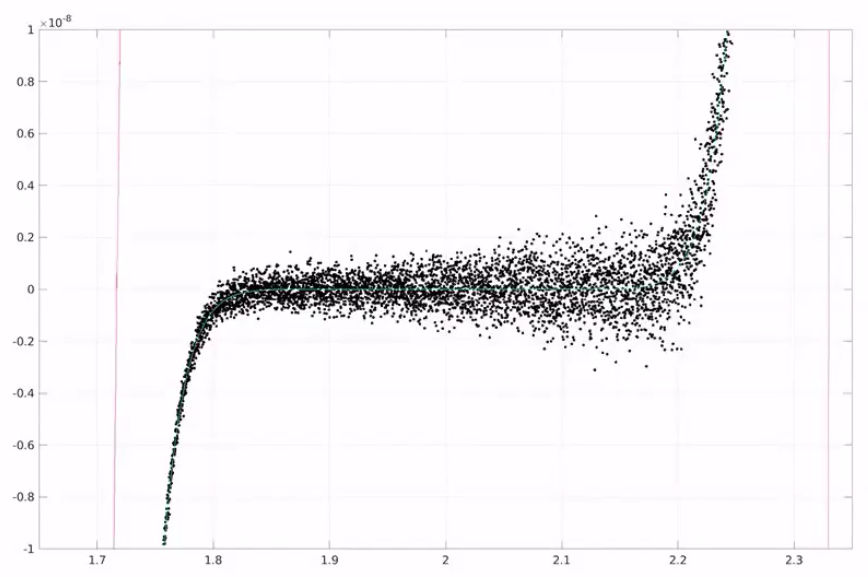
\includegraphics[width = 7cm]{images/lec2-1.png}
    \caption{\textit{MATLAB} demo}
\end{figure}

Picture \ref{fig:2-1} is a foreshadowing of what will happen in linear algebra: The vertical axis is the number of correct digits, 
both actual (the black dots) and lower-bounded using our error bound (the red curve). The horizontal axis is the problem we are trying to solve,
in this simple case the value of $x$ at which we are evaluating a fixed polynomial $p(x)$. 

\begin{figure}[h]
    \centering
    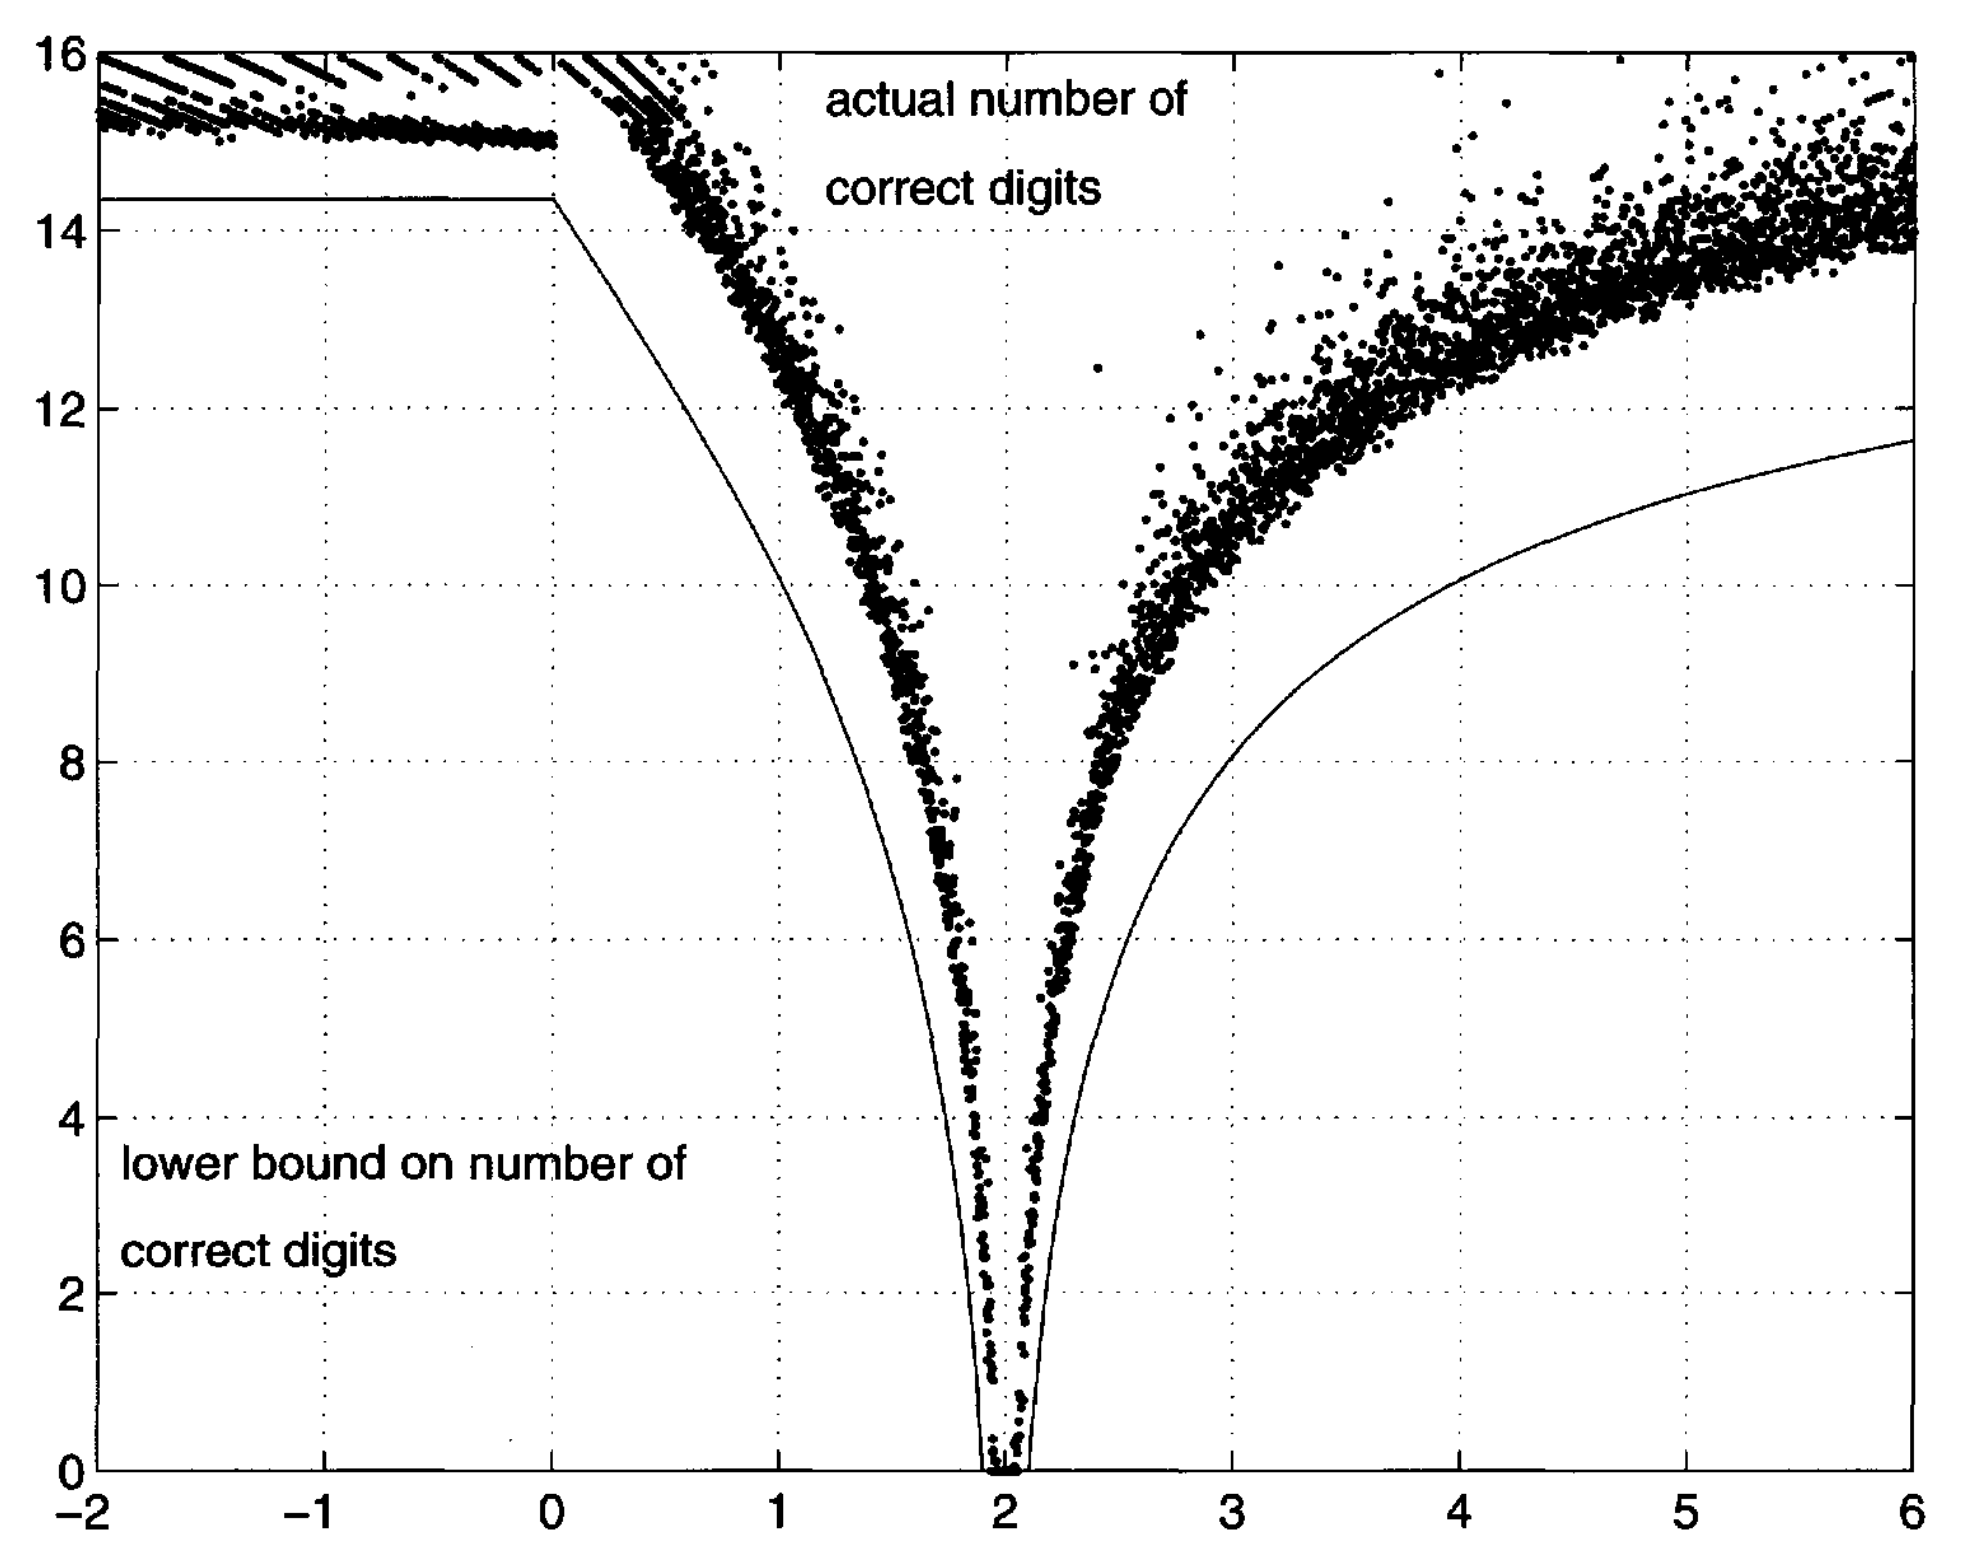
\includegraphics[width = 7cm]{images/lec2-2.png}
    \caption{Plot of error bounds on the value of $y = (x - 2)^9$ evaluated using \textit{Horner's Rule}.}
    \label{fig:2-1}
\end{figure}

The number of correct digits gets smaller and smaller, until no leading correct digits are computed, the closer the problem gets to the hardest possible problem, 
in this case the root $x=2$ of the polynomial. This is the hardest problem because the only way to get a small relative error in the solution $p(2)=0$, 
is to compute 0 exactly, i.e. no roundoff is permitted. And changing $x$ very slightly makes the answer $p(x)$ change a lot, relatively speaking. 
In other words, the condition number, $\sum_i |a_i x^i| / |p(x)|$ in this simple case, approaches infinity as $p(x)$ approaches zero.

In linear algebra the horizontal axis still represents the problem being solved, but since the problem is typically defined by an $n \times n$ matrix, 
we need $n^2$ axes to define the problem. There are now many "hardest possible problems", e.g. singular matrices if the problem is matrix inversion. 
The singular matrices form a set of dimension $n^2-1$ in the set of all matrices, the surface defined by $\operatorname{det}(A)=0$. And the closer the matrix is to this set, 
i.e. to being singular, the harder matrix inversion will be, in the sense that the error bound will get worse and worse the closer the matrix is to this set. 
Later we will show how to measure the distance from a matrix to the nearest singular matrix "exactly" (i.e. except for roundoff) using the SVD, 
and show that the condition number, and so the error bound, is inversely proportional to this distance.

Here is another way the above figure foreshadows linear algebra. Recall that we could interpret the computed value of the polynomial
$p(x) = \sum_i a_i x^i$, with roundoff errors, as the exactly right value of a slightly wrong polynomial, that is \begin{align*}
    p_{\operatorname{alg}(x)} = \sum_{i=0}^{d} [(1+e_i) a_i]x^i,
\end{align*}
where $|e_i| \leq 2d \varepsilon$. We called this property "backward stability", in contrast to "forward stability" which would means that the answer itself is close to correct. 
So the error bound bounds the difference between the exact solutions of two slightly different problems $p(x)$ and $p_{\operatorname{alg}(x)}$.

For most linear algebra algorithms, we will also show they are backward stable. For example, if we want to solve $Ax=b$, we will instead get the exact solution of $(A+E)\hat{x} = b$, 
where the matrix $E$ is "small" compared to $A$. Then we will get error bounds by essentially taking the first term of a Taylor expansion of $(A+E)^{-1}$:\begin{align*}
    \hat{x} - x = (A+E)^{-1}b - A^{-1}b
\end{align*}
To do this, we will need to introduce some tools like matrix and vector norms (so we can quantify what "small" means) in the next lecture.

To extend the analysis of \textit{Horner's Rule} to linear algebra algorithms, note the similarity between \textit{Horner's Rule} and computing dot-products: \begin{align*}
    \begin{array}{lll}
        p=a_d & \text{for } i = d-1:-1:0 & p=xp + a_i \\
        s=0 & \text{for } i = 1:d & s=x_i y_i + s
    \end{array}
\end{align*}
Thus the error analysis of dot products, matrix multiplication, and other algorithms is very similar.

\subsection{Details on Floating Point and Error Analysis}
Next we briefly discuss some properties and uses of floating point that go beyond these most basic properties (even more details are at the end of these notes). 
Analyzing large, complicated codes by hand to understand all these issues is a challenge, so there is research in automating this analysis; 
there is a day-long tutorial on available tools that was held at \textit{Supercomputing'19}.

\subsubsection{Exception Handling}
\begin{itemize}
    \item Underflow: $\mathrm{Tiny} / \mathrm{Big} = 0$,  (or "subnormal", special numbers at bottom of exponent range)
    \item Overflow and Divide-by-Zero:  $1/0 = \mathrm{Inf} = \text{"infinity"}$, represented as a special case in the usual format
    \item Natural computational rules: $\mathrm{Big} + \mathrm{Big} = \mathrm{Inf}$, $\mathrm{Big} \cdot \mathrm{Big} = \mathrm{Inf}$, $3 - \mathrm{Inf} = -\mathrm{Inf}$, etc.
    \item Invalid Operation: $0/0 = \mathrm{NaN} = \text{"Not a Number"}$, also represented as special case: $\mathrm{Inf} - \mathrm{Inf} = \mathrm{NaN}$,
    $\sqrt{-1} = \mathrm{NaN}$, $3 + \mathrm{NaN} = \mathrm{NaN}$, etc. Flags are available to check if such exceptions occurred.
\end{itemize}

Impact on software: \begin{itemize}
    \item Reliability: Suppose we want to compute $s=\sqrt{\sum_{i=1}^{n}\left|x_{i}\right|^{2}}$: What could go wrong with:\begin{algorithmfrm}
        \begin{algorithmic}[1]
            \State $s=0$
            \For{\texttt{$i=i:n$}}
                \State $s = s + x_i^2$
                \EndFor
            \State $s = \sqrt{s}$
        \end{algorithmic}
    \end{algorithmfrm}
    To see how standard libraries deal with this, see \textit{snrm2.f} in the \href{http://bebop.cs.berkeley.edu/reproblas}{\textit{BLAS}}.
    For a worst-case example, see \href{https://people.eecs.berkeley.edu/~demmel/ma221_Fall04/ariane5rep.html}{Ariane 5 crash}.
    We are currently investigating how to automatically guarantee that libraries like \textit{LAPACK} cannot "misbehave" because of exceptions 
    (go into infinite loops, give wrong answer without warning, etc.)
    \item Error analysis: it is possible to extend error analysis to take underflow into account by using the formula 
    \begin{align*}
        \operatorname{rnd}(a \odot b) = (1+\delta)(a \odot b) + \eta
    \end{align*}
    where $|\delta| \leq \varepsilon$ as before, and $|\eta|$ is bounded by a tiny number, depending on how underflow is handled.
    \item Speed: Run "reckless" algorithm that is fast but ignores possible exceptions. Check flags to see if exception occurred.
    In rare case of exception, rerun with slower, more reliable algorithms.
\end{itemize}

\subsubsection{Higher Precision Arithmetic}
Possible to simulate using either fixed or floating point, various packages available: 
\href{http://mpfr.org/}{\textit{MPFR}}, 
\href{http://crd.lbl.gov/~dhbailey/mpdist/index.html}{\textit{ARPREC}},
\href{http://www.netlib.org/xblas}{\textit{XBLAS}}. 
There are also special fast tricks just for high precision summation.

\subsubsection{Lower Precision Arithmetic}
Lower precision arithmetic: As mentioned before, many companies are building hardware accelerators for machine learning, which means they provide fast matrix multiplication. 
As mentioned in Lecture 1, and will be discussed later, it is possible to reformulate many dense linear algebra algorithms to use matrix multiplication as a building block, 
and so it is natural to want to use these accelerators for other linear algebra problems as well. As illustrated in our error analysis of \textit{Horner's Rule}, 
many of our error bounds will be proportional to $d\varepsilon$, where $d$ is the problem size (e.g. matrix dimension), and often $d^2 \varepsilon$ or more. 
These bounds are only useful when $d \varepsilon$ (or $d^2 \varepsilon$) are much smaller than $1$.
So when $\varepsilon$ is about $4\mathrm{e}-3$ with \textit{bfloat16}, this means $d$ must be much smaller than $1/\varepsilon = 256$, 
or much smaller than $1/\sqrt{\varepsilon} = 16$, for these bounds to be useful. This is obviously very limiting, and raises several questions:
Are our (worst case) error bounds too pessimistic? Can we do most of the work in low precision, and little in high precision, to get an accurate answer? 
There are some recent positive answers to both these questions.

\subsubsection{Variable Precision}
There have been various proposals over the years to support variable precision arithmetic, sometimes with variable word lengths, 
and sometimes encoded in a fixed length word. Variable word lengths make accessing arrays difficult. There has been recent interest in this area, 
with variable precision formats called \textit{unums} (variable length) and posits (fixed length), proposed by John Gustavson. 
Posits allocate more bits for the mantissa when the exponent needs few bits (so the number is not far from 1 in magnitude) 
and fewer mantissa bits for long exponents. This so-called "tapered precision" complicates error analysis, 
and it is an open question of how error analyses or algorithms could change to benefit. 
See the class webpage for links to more details, including a \href{https://www.youtube.com/watch?v=LZAeZBVAzVw}{youtube video} of a debate between Gustavson and
Kahan about the pros and cons of \textit{unums}.

\subsubsection{Reproducibility}
Almost all users expect that running the same program more than once gives the bitwise identical answer; this is important for debugging, correctness, 
even legal reasons sometimes. But this can no longer be expected, even on your multicore laptop, because parallel computers (so nearly all now),
may execute sums in different orders, and roundoff makes summation nonassociative: \begin{align*}
    (1-1)+1\mathrm{e}-20 = 1\mathrm{e}-20 \neq 0 = (1+1\mathrm{e}-20)-1
\end{align*}
There is lots of work on coming up with algorithms that fix this, without slowing down too much, such as \href{http://bebop.cs.berkeley.edu/reproblas}{ReproBLAS}.
The \href{http://754r.ucbtest.org/background/ieee-computer.pdf}{2019 version} of the IEEE 754 standard also added a new "recommended instruction", 
to accelerate both the tricks for high precision arithmetic, and to make summation associative.

\subsubsection{Guaranteed Error Bounds from Interval Arithmetic}
Represent each floating point number by an interval $[x_{\mathrm{low}},x_{\mathrm{high}}]$, 
and use special rounding modes in IEEE standard to make sure that lower and upper bounds are maintained throughout the computation: \begin{align*}
    [x_{\mathrm{low}},x_{\mathrm{high}}] + [y_{\mathrm{low}},y_{\mathrm{high}}] = [\operatorname{round\_down}(x_{\mathrm{low}} + y_{\mathrm{low}}) + \operatorname{round\_up}(x_{\mathrm{high}} + y_{\mathrm{high}})]
\end{align*}
Drawback: naively replacing all variables by intervals like this often makes interval widths grow so fast that they are useless.
There have been many years of \href{http://www.ti3.tu-harburg.de/rump/}{research} on special algorithms that avoid this, especially for linear algebra.

\subsubsection{Exploiting Structure to get High Accuracy}
Some matrices have special mathematical structure that allows formulas to be used where roundoff is provably bounded so that you get high relative accuracy, 
i.e. most leading digits correct. For example, a Vandermonde matrix has entries $V_{ij} = x_i^j$, and arises naturally from polynomial interpolation problems. 
It turns out that this special structure permits many linear algebra problems, even eigenvalues, to be done accurately, 
no matter how hard ("ill-conditioned") the problem is using conventional algorithms. See \href{http://journals.cambridge.org/abstract_S0962492906350015}{"Accurate and efficient expression evaluation and linear algebra"} for details.

\newpage
\section{Lecture 3: Norms, the SVD, and Condition Numbers}
\subsection{Accuracy}
To summarize our approach to understanding accuracy in the face of roundoff (or other) error, our goal will be to prove that algorithms are "backward stable". 
For example if our algorithm for computing the scalar function $f(x)$:
$$\mathrm{alg}(x)=f(x+\delta) \sim f(x) + f^\prime(x)\delta$$
where $\delta$ is small compared to $x$. Then relative error can be approximated by:
\begin{align*}
    \underbrace{\left| \frac{\operatorname{alg}(x) - f(x)}{f(x)} \right|}_{\text{relative \ error\ in\ output}} &\leq  \left| \frac{f'(x) \delta}{f(x)} \right| \\ 
    &= \underbrace{\left| \frac{f'(x) x}{f(x)} \right|}_{\text{condition number}} \underbrace{\left|\frac{\delta}{x} \right|}_{\text{relative\ error\ in\ input}} \\
\end{align*}

\begin{definition}
    The factor $\left| \frac{f'(x) x}{f(x)} \right|$ is called the condition number of the function $f$ evaluated at $x$.
\end{definition}
Same approach for solving $Ax=b$, but where we get $(A+\Delta)\hat{x}=b$ instead, where $\Delta$ is small compared to $A$. 

To formalize the notion of "small", we need to understand vector and matrix norms. In both cases, we may say we want to compute $x=f(A)$, 
but get $\mathrm{alg}(x)=\hat{x}=f(A+\Delta)$. So to bound the error, we write \begin{align*}
    \mathrm{error}=\hat{x}-x=f(A+\Delta)-f(A).
\end{align*}
Assuming $\Delta$ is small enough for \textit{Taylor expansion}, we get \begin{align*}
    \mathrm{error} \sim J_f(A)\Delta
\end{align*}
where $J_f(A)$ is the Jacobian of $f$. If $A$ and $x$ were scalars, we could take absolute values and get an absolute error bound: \begin{align*}
    \|\mathrm{error}\| \lessapprox \|J_f(A)\| \|\Delta\|
\end{align*}
and proceed as above.

In the cases most relevant to linear algebra, $A$ and $x$ are not scalars but matrices and vectors (with obvious generalizations, depending on the problem). 
To generalize this error bound, we need to generalize absolute values, which leads us to norms.

\subsection{Matrix and Vector Norms}
\begin{definition}[Inner Product]
    Let $\mathcal{B}$ be a real linear space. $<\cdot,\cdot>:\mathcal{B}\times \mathcal{B} \rightarrow \mathbb{R(C)}$ 
    is an inner product if all of the following apply:
    \begin{enumerate}
        \item $<x,y>=<y,x>$
        \item $<x,y+z>=<x,y>+<x,z>$
        \item $<\alpha x,y>=\alpha<x,y>$ for any scalar $\alpha$
        \item $<x,x>\geq 0$, and $<x,x>=0$ iff $x=0$
    \end{enumerate}
\end{definition}

\begin{lemma}
    Cauchy-Schwartz inequality: $|<x,y>|\leq \sqrt{<x,x>\dot <y,y>}$
\end{lemma}

\begin{definition}[Norm]
    Let $\mathcal{B}$ be a real (complex) linear space $\mathbb{R}^n$ (or $\mathbb{C}^n$). It is normed if there is a function $||\cdot ||:\; \mathcal{B}\rightarrow \mathbb{R}$ satisfying all of the following:
    \begin{enumerate}
        \item positive definiteness: $\norm{x} \geq 0$ and $\norm{x} = 0$ if and only if $x=0$
        \item homogeneity: $\norm{cx} = |c| \norm{x}$
        \item the triangle inequality: $\norm{x+y} \leq \norm{x} + \norm{y}$
    \end{enumerate}
\end{definition}

\begin{savenotes}
    \begin{example}
        The most common norms:
        \begin{itemize}
            \item \textit{p-norms}: $||x||_p=(\sum |x_i|^p)^{1/p}$
            \item \textit{Euclidean norm}: $2$-norm\footnote{If $x$ is real, then $\sqnorm{x}=\sum_{i=1}^n x_i^2 = x^\top x$}
            \item \textit{infinity-norm}: $||x||_\infty=\max_i |x_i|$
            \item \textit{C-norm}: $||Cx||$ where $C$ is any nonsingular matrix
        \end{itemize}
    \end{example}
\end{savenotes}

\begin{lemma}
    All norms are equivalent, i.e. given any $||\cdot||_a$ and $||\cdot||_b$, there are positive constants $\alpha$ and $\beta$ such that \begin{align*}
        \alpha ||\cdot||_a \leq ||\cdot||_b \leq \beta ||\cdot||_a
    \end{align*}
    \begin{proof}
        Compactness.
    \end{proof}
\end{lemma}

\begin{definition}[Matrix Norm]
    \begin{enumerate}
        \item[]
        \item $\norm{A} \geq 0$ and $\norm{A}=0$ if and only if $A=0$
        \item $\norm{cA} = |c|\norm{A}$
        \item $\norm{A+B} \leq \norm{A} + \norm{B}$
    \end{enumerate}
\end{definition}

\begin{example}
    \begin{itemize}
        \item[]
        \item Max norm: $\max_{ij} |A_{ij}|$
        \item Frobenius norm: $\|A\|_{F} = \left(\sum\left|a_{i j}\right|^{2}\right)^{1 / 2}$
    \end{itemize}
\end{example}

\begin{definition}[Operator Norm]
    Given any vector norm, $\|A\|=\max _{x \neq 0} \frac{\| A_{x} \|}{\|x\|}$
\end{definition}

\begin{lemma}
    An operator norm is a matrix norm.
\end{lemma}

\begin{lemma}
    If $\|A\|$ is an operator norm, then there exists $x$ such that $\|x\|=1$ and $\|Ax\|=\|A\|$.
    \begin{proof}
        \begin{align*}
            \|A\| &= \max _{x \neq 0} \frac{\| A_{x} \|}{\|x\|} \\
            &= \max _{x \neq 0} \| A (x/\|x\|) \| \\
            &= \max _{\text{unit\ vectors}\ y} \| A y \| \\
        \end{align*}
        $y$ attaining max exists since $\|Ay\|$ is a continuous function of $y$ on compact (closed and bounded) set (unit ball).
    \end{proof}
\end{lemma}

\begin{lemma}
    \begin{align*}
        ||x||_2 \ \leq \ &||x||_1 \ \leq \ \sqrt{n}||x||_2,\\
        ||x||_\infty \ \leq \ &||x||_2 \ \leq \ \sqrt{n}||x||_\infty,\\
        ||x||_\infty \ \leq \ &||x||_1 \ \leq \ n||x||_\infty,\\
    \end{align*}
\end{lemma}

\begin{definition}
    The norms are called mutually consistent if $||A\cdot B||_{m\times p}\leq ||A||_{m\times n}\cdot ||B||_{n\times p}$.
\end{definition}

\subsection{Orthogonal and Unitary Matrices}
Notation: $Q^{*}=\overline{\left(Q^{\top}\right)}$, sometimes we write $Q^H$, $H$ stands for \textit{Hermitian}.
\begin{definition}[Orthogonal]
    $Q$ square, real, $Q^{-1}=Q^{\top}$
\end{definition}
\begin{definition}[Unitary]
    $Q$ square, complex, $Q^{-1}=Q^{*}$
\end{definition}
\begin{fact}
    $Q$ orthogonal $\Longleftrightarrow \ Q^{\top} Q=I$ $\Longleftrightarrow$ all columns of $Q$ are pairwise orthogonal and unit vectors.
    $QQ^\top = I$ implies same about rows.
\end{fact}

\begin{theorem}[Pythagorean Theorem]\label{thm:pythagorean}
    $\left\|Qx\right\|_2 = \| x \|_{2}$
    \begin{proof}
        \begin{align*}
            \left\|Qx\right\|_2  &= \left(Q_{X}\right)^{\top} Q_{X} \\
            &= x^{\top} x \\
            &= \| x \|_{2}
        \end{align*}
    \end{proof}
\end{theorem}
\begin{fact}
    $Q$, $Z$ orthogonal implies that $QZ$ orthogonal.
    \begin{proof}
        \begin{align*}
            (Q Z)^{\top}(Q Z)= Z^\top Q^\top QZ = Z^\top Z = I
        \end{align*}
    \end{proof}
\end{fact}

\begin{fact}
    if $Q$ is $ m \times n$, $n<m$ and $Q^{T} Q=I_{n}$, then you can add $m-n$ columns to $Q$, to make it square and orthogonal.
\end{fact}

\begin{lemma} % 1.8
    \begin{enumerate}
        \item[]
        \item $||Ax|| \leq ||A|| ||x||$ for a vector norm and its operator norm
        \item $||AB|| \leq ||A||||B||$ for any operator norm or for the Frobenius norm.
        \item The max norm and Frobenius norm are not operator norms.
        \item $||QAZ||=||A||$ if $Q$ and $Z$ are orthogonal or unitary for the Frobenius norm and for  and for the operator norm induced by $||\cdot||_2$
        \item Maximum absolute row sum: $\|A\|_{\infty} \equiv \max _{x\neq 0} \frac{\|A x\|_{\infty}}{\|x\|_{\infty}}=\max _{i} \sum_{j}\left|a_{i j}\right|$
        \item Maximum absolute col sum: $\|A\|_{1} \equiv \max _{x\neq 0} \frac{\|A x\|_{1}}{\|x\|_{1}}=\left\|A^{T}\right\|_{\infty}=\max _{j} \sum_{i}\left|a_{i j}\right|$
        \item $\|A\|_{2} \equiv \max _{x\neq 0} \frac{\|A x\|_{2}}{\|x\|_{2}}=\sqrt{\lambda_{\max }\left(A^{*} A\right)}$
        \begin{proof}
            With the fact that $A^\top A$ symmetric implies that there is eigendecomposition $A^\top Aq_i=\lambda_iq_i$, where $\lambda_i$ real, 
            $q_i$ all unit orthogonal vectors. $A^{\top}A=Q\Lambda Q^{\top}$:
            \begin{align*}
                \|A \|_{2} &= \max _{x\neq 0} \frac{\|A x\|_{2}}{\|x\|_{2}} \\
                &= \max _{x\neq 0}\frac{\sqrt{(A x)^{\top}(A x)}}{\sqrt{x^{\top} x}} \\
                &= \max _{x\neq 0} \sqrt{\frac{x^{T} A^{T} A x}{x^{\top} x}} \\
                &= \sqrt{\max _{x \neq 0} \frac{x^{\top} Q\Lambda Q^{\top} x}{x^{\top} Q \underbrace{Q^{\top} x}}_{y}} \\
                &= \sqrt{\max _{y \neq 0} \frac{y^{\top}\Lambda y}{y^{\top} y}} \\
                &= \sqrt{\max _{y \neq 0} \frac{\sum \lambda_{i} y_i^2}{\sum y_i^2}} \\
                &\leq \sqrt{\max _{y \neq 0} \frac{\lambda_{\mathrm{max}} \sum y_i^2}{\sum y_i^2}} \\
            \end{align*}
        \end{proof}
        \item $\|A\|_{2}=\left\|A^{\top}\right\|_{2}$
        \item $\|A\|_{2}=\max _{i}\left|\lambda_{i}(A)\right|$ if $A$ is normal, i.e., $A A^{*}=A^{*} A$.
        \item If A is n-by-n, then \begin{align*}
            \begin{array}{l}
                n^{-1 / 2}\|A\|_{2} \leq\|A\|_{1} \leq n^{1 / 2}\|A\|_{2} \\
                n^{-1 / 2}\|A\|_{2} \leq\|A\|_{\infty} \leq n^{1 / 2}\|A\|_{2} \\
                n^{-1}\|A\|_{\infty} \leq\|A\|_{1} \leq n\|A\|_{\infty} \\
                n^{1 / 2}\|A\|_{1} \leq\|A\|_{F} \leq n^{1 / 2}\|A\|_{2}
            \end{array}
        \end{align*}
        \item $\|Q\|_{2}=1$ if $Q$ orthogonal
    \end{enumerate}
\end{lemma}

\subsection{Singular Value Decomposition}
The SVD is a Swiss Army Knife of numerical linear algebra. Given SVD, one can easily \begin{itemize}
    \item solve $Ax=b$;
    \item solve overdetermined or underdetermined least squares problems with rectangular $A$ (whether $A$ full rank or not);
    \item compute eigenvalues and eigenvectors of $AA^\top $, $A^\top A$;
    \item compute eigenvalues and eigenvectors of $A=A^\top$.
\end{itemize}   
Furthermore, one can use the SVD to write down error bounds for all these problems. It is more expensive to compute than other algorithms specialized for these problems, 
so it may not be the algorithm of first resort.

\begin{theorem}
    Suppose $A$ is an $ m \times m$ matrix. Then there an exists orthogonal matrix $U=\left[u_1, \cdots, u_m\right]$, 
    a diagonal matrix $\Sigma=\operatorname{diag}\left(\sigma_1, \cdots, \sigma_m\right)$, $\sigma_1 \geq \sigma_2 \geq \cdots \geq \sigma_m \geq 0$,
    and an orthogonal matrix $V=\left[v_1, \cdots, v_m\right]$ such that $A=U\Sigma V^\top$.

    More generally, $A$ is an $ m \times n$ matrix, where $m>n$, $U$ is an $ m \times m$ matrix and is orthogonal as before, $V$ is a $ n \times n$, orthogonal matrix,
    $\Sigma$ is an $ m \times n$ matrix with same diagonal. When $m>n$, sometimes write as following (thin SVD): \begin{align*}
        A = \left[ u_1, \cdots, u_n \right] \operatorname{diag}\left(\sigma_1, \cdots, \sigma_n\right) V^\top
    \end{align*}

    Geometric interpretation: $A$ is a linear mapping from $\mathbb{R}^n\rightarrow \mathbb{R}^m$ with right orthogonal bases of $\mathbb{R}^n$ and $\mathbb{R}^m$, $A$ is diagonal, $Av_i=\sigma_{i} u_(i)$
    \begin{proof}
        induction on $n$. 2 base cases:

        $n=1$: Let $U$ have first column $=A/\|A\|_2$, other columns chosen in any way that makes $U$ orthogonal, $\sigma_1=\|A\|_2$, $v=1$

        $A=O$: $U=I_{m}$, $\Sigma=O$, $V=I_{n}$

        Induction step (if $A \neq 0$)
        \begin{align*}
            \|A\|_2 &= \max _{x \neq 0} \|Ax\|_2 / \|x\|_2 \\
            &= \max _{\|x\|_2=1}  \|Ax\|_2
        \end{align*}
        Let $v_1$ be x attaining max, $\sigma_1= \|A\|_2= \|Av_1\|_2$, $vu1=Av_1/ \|Av_1\|_2$. $V=\left[v_1, \hat{V}\right]$, $U=\left[u_1, \hat{U}\right]$, both square and orthogonal.
        \begin{align*}
            \hat{A} &=U^{\top} A V\\
            &= \left[\begin{array}{c}
                u_1^{\top} \\
                \hat{U}^{\top}
                \end{array}\right] A[v_1, \hat{V}]\\
                &= \left[\begin{array}{ll}
                    v_1^{\top} A v_1 & u_1^{\top} A \hat{V} \\
                    \hat{U}^{\top} A v_1 & \hat{U}^{\top} A \hat{V} 
                    \end{array}\right]\\
                &= \left[\begin{array}{cc}
                    \sigma_{1} & A_{12} \\
                    A_{21} & A_{22}
                    \end{array}\right]
        \end{align*}
        $A_{21}=0$ by definition of $\hat{U}$, $A_{12}=0$ by definition of $\sigma_1=\|A\|_2$.

        Use induction on $A_{22}=V_{2} \sum_{2} V_{2}^{T}$.
        \begin{align*}
            A &= U \hat{A} V^\top \\
            &= U \left[\begin{array}{cc}
                \sigma_{1} & A_{12} \\
                A_{21} & A_{22}
                \end{array}\right] V^\top
        \end{align*}
    \end{proof}
\end{theorem}

\subsection{Useful Properties of SVD}
\begin{fact}
    $A$ is $m \times m$, nonsingular, we can solve $Ax=b$ using SVD in $O(n^2)$ move operations.
    \begin{proof}
        \begin{align*}
            x=A^{-1} b=\left(U \Sigma v^{T}\right)^{-1} b=V\left(\Sigma^{-1}\left(U^{\top} b\right)\right)
        \end{align*}
    \end{proof}
    But note: computing the SVD itself is expensive ($O(n^3)$). If all you want to do is solve $Ax=b$, Gaussian Elimination is cheaper. 
    On the other hand, we will see that the SVD is more reliable when $A$ is nearly singular, provides and error bound, 
    and even lets us "solve" $Ax=b$ when $A$ is exactly singular.
\end{fact}

\begin{fact}
    When $m>n$, solve $\underset{x}{\arg\min} \|Ax-b\|_2$ use thin SVD $A=U \Sigma V^{\top}$, then \begin{align*}
        x=V\Sigma^{-1}U^\top b.
    \end{align*}
    \begin{proof}
        $A=\hat{U} \hat{\Sigma} V^{\top}$,
        $\hat{U}=\left[U, U^{\prime}\right]$, square and orthogonal
        $\hat{\Sigma}=\left[\begin{array}{l}
            \Sigma \\
            0
            \end{array}\right]$.
        \begin{align*}
            \|A x-b\|_{2}^{2} &= \| \hat{U} \hat{\Sigma} V^{\top} x-b \|_{2}^{2} \\
            &= \| \hat{U}^{\top}(\hat{U} \hat{\Sigma} V^{\top} x-b) \|_{2}^{2} \\
            &= \left\|\hat{\Sigma} V^{\top} x-\hat{U}^{\top} b\right\|_{2}^{2} \\
            &= \left\| \left[\begin{array}{ccc}
                \Sigma V^{\top} x & -U^{\top} b \\
                & -U^{\prime T} b
                \end{array}\right] \right\|_2^2 \\
            &= \left\|\Sigma V^{\top} x-U^{\top} b\right\|_{2}^{2} + \| V^{\prime \top} b \|_{2}^{2}
        \end{align*}
        Easy to minimize by choosing $x=V \Sigma^{-1} U^{\top } b$ to zero out the term depending on $x$.
    \end{proof}
\end{fact}

\begin{definition}[Moore-Penroso pseudoinverse]
    For $A=U \Sigma V^{\top}$ and is full rank, $$A^{+}=V \Sigma^{-1} U^{\top }.$$
\end{definition}

This is the most natural extension of the definition of "inverse" to rectangular full-rank matrices. We can also use the SVD, 
and an appropriately defined Moore-Penrose pseudoinverse to solve the rank deficient least squares problems, or underdetermined problem ($m < n$), 
as we describe later.

Just to solve a least squares problem where you are not worried about rank deficiency, the QR decomposition is cheaper.
On the other hand, we will see that the SVD is more reliable when $A$ is nearly singular.

\begin{fact}
    $A$ symmetric with eigenvalues $\Lambda=\mathrm{diag}(\lambda_1, \cdots, \lambda_n)$. Then SVD of $A$ is 
    \begin{align*}
        A&=V \Lambda V^{\top } \\
        &= (V D)(D \Lambda) \cdot V^{\top} \\
        &= U \Sigma V^{\top }
    \end{align*}
    where $D=\mathrm{diag}(\mathrm{sign}(\lambda_i))$.
\end{fact}
\begin{fact}
    Using thin SVD,
    \begin{align*}
        A^\top A= (U \Sigma V^{T})^{\top}(U \Sigma V^{T})=V\Sigma^2V^\top 
    \end{align*}
\end{fact}
\begin{fact}
    Using thin SVD,
    \begin{align*}
        AA^\top  = (U \Sigma V^{T})(U \Sigma V^{T})^{\top}=U\Sigma^2U^\top 
    \end{align*}
    That means there are a bunch implicitly zero eigenvalues that not writing down their eigenvectors. 
    It would be a perfectly adequate way to do if you only care about the space spanned by the nonzero eigenvectors.
\end{fact}

\begin{fact}
    Let $H=\left[\begin{array}{ll}
        0 & A^{\top} \\
        A & 0
        \end{array}\right]$. Then H has eigenvalues $\pm \sigma_i$ and eigenvectors $\frac{1}{\sqrt{2}}\left[\begin{array}{c}
            v_c \\
            \pm u(i)
            \end{array}\right]$
    \begin{proof}
        Plug in $A=U \Sigma V^{\top}$ into $H$.
    \end{proof}
\end{fact}

\begin{fact}
    Suggests that algorithms for SVD and symmetric eigenproblem will be closely related.
\end{fact}

\begin{fact}
    $\|A\|_2=\sigma_1$, $\|A^{-1} \|_{2}=\frac{1}{\sigma_{n}}$.
\end{fact}

\begin{definition}[Condition number]
    $\kappa(A)=\frac{\sigma_1}{\sigma_n}$
\end{definition}

\begin{fact}
    Let $S$ be unit sphere in $\mathbb{R}^n$. Then $AS$ is an ellipsoid centered at $O$ with principal axes $\sigma_i$, $u_i$.
    \begin{proof}
        Suppose $s=\left[s_{1}, \ldots, s_{n}\right]$ where $\|s\|_{2}=0$, and write
        \begin{align*}
            As=U\Sigma V^{\top}s=U\Sigma \hat{s} = \Sigma u_i \sigma_i \hat{s}_i
        \end{align*}
    \end{proof}
\end{fact}

\begin{example}
    $U_{1}=\left[\begin{array}{l}
        1 \\
        0
        \end{array}\right]$, $U_{2}=\left[\begin{array}{l}
            0 \\
            1
            \end{array}\right]$, $\left[\begin{array}{l}
                x \\
                y
                \end{array}\right]=\left[\begin{array}{l}
                \sigma_{1} \hat{s}_{1} \\
                \sigma_{2} \hat{s}_{2}
                \end{array}\right]$,
    $$\left(\frac{x}{\sigma_{1}}\right)^{2}+\left(\frac{y}{\sigma_{2}}\right)^{2}=\hat{s}_{1}^{2}+\hat{s}_{2}^{2}=1$$
\end{example}

\begin{fact}
    Suppose $\sigma_1 \geq \sigma_{2} \geq \cdots \geq \sigma_r > 0 = \sigma_{r+1}= \sigma_{r+2}= \cdots = \sigma_{n}$. Then $A$ has rank $r$;
    the null space of $A$ is $A=\operatorname{span}\left(v_{r+1}, \cdots, v_n\right)$;
    the range space of $A$ is $A\ = \ \operatorname{span}\left(v_{1}, \cdots, v_r\right)$.
\end{fact}

\begin{fact}
    Matrix $A_k$ of rank $k$ closest to $A$ in $2$-norm is \begin{align*}
        A_{k}=\sum_{c=1}^{k} v_{i} \sigma_{i} v_{i}^{\top}=U\Sigma_kV^\top ,
    \end{align*}
    where \begin{align*}
        \Sigma_k = \text{diag}\left(\sigma_1, \sigma_{2}, \cdots , \sigma_k, 0, \cdots,0\right),
    \end{align*}
    and the distance is \begin{align*}
        \|A_k -A\|_2=\sigma_{k+1}.
    \end{align*}
    In particular, the closest non-full rank matrix to $A$ is at distance $\sigma_n=\sigma_{\mathrm{min}}$.
    \begin{proof}
        Easy to see $A_k$ has right rank, right distance to $A$, $\sigma_{k+1}$. Need to show $A_k$ is the closest. Suppose $B$ has rank $k$, 
        so the null space of $B$ has dimension $n-k$. The space spanned by the $\{v_1,\cdots,v_{k+1}\}$ has dimension $k+1$.
        Since the sum of the dimensions of spaces $(n-k)+(k+1)=n+1>n$, these two spaces intersect in unit vector $h$. Then \begin{align*}
            \|A-B\|_{2} &\geq \|(A-B) \mathbf{h}\|_{2} \\
            &= \norm{U\Sigma V^\top h}_2 = \norm{\Sigma V^\top h}_2 \\
            &= \norm{\Sigma \left[ x_1, \cdots, x_{k+1}, 0, \cdots, 0 \right]^\top}_2 \\
            &\geq \sigma_{k+1}
        \end{align*}
    \end{proof}
\end{fact}

\subsection{Condition Number}
Now we start using this material to analyze the condition number for matrix inversion and solving $Ax=b$: If $A$ (and $b$) change a little bit, 
how much can $A^{-1}$ (and $x=A^{-1} b$) change?

If $|x|<1$, recall that \begin{align*}
    \frac{1}{1-x}=1+x+x^{2}+x^{3}+\cdots
\end{align*}
Now generalize to matrices.

\begin{lemma}
    If operator $\norm{X}<1$, then $I-X$ is nonsingular and \begin{align*}
        (I-X)^{-1}=\sum_{i=0}^{\infty} x^{i}, \ \norm{(I-X)^{-1}} \leq \frac{1}{1 - \norm{X}}
    \end{align*}
    \begin{proof}
        Claim $I + X + X^2 + \cdots$ converges:
        \begin{align*}
            \norm{X^i} \leq \norm{X}^i \rightarrow 0
        \end{align*}
        as $i \rightarrow \infty$. So by equivalence of norms there is some $C>0$ such that \begin{align*}
            \max_{kj} | (X^i)_{kj} | \leq C \norm{X^i} \leq C \norm{X}^i
        \end{align*}
        and so $kj$-th entry of $I + X + X^2 + \cdots$ is dominated by a convergent geometric series and so converges.
        Claim that \begin{align*}
            (I-X)\left(I+X+X^{2}+\cdots+X^{i}\right) = I - X^{i+1} \rightarrow I
        \end{align*}
        as $i \rightarrow \infty$. \begin{align*}
            \norm{I + X + X^2 + \cdots} &\leq \norm{I} + \norm{X} + \norm{X^2} + \cdots && \text{by triangle inequality} \\
            &\leq \norm{I} + \norm{X} + \norm{X}^2 + \cdots && \text{by }\norm{AB} \leq \norm{A} \norm{B} \\
            &= 1 + \norm{X} + \norm{X}^2 + \cdots && \\
            &= \frac{1}{1 - \norm{X}} &&
        \end{align*}
    \end{proof}
\end{lemma}

\begin{lemma}
    Suppose $A$ invertible. Then $A-E$ invertible if \begin{align*}
        \norm{E} < \frac{1}{\norm{A^{-1}}},
    \end{align*}
    in which case \begin{align*}
        (A-E)^{-1} = Z + Z(EZ) + Z(EZ)^2 + Z(EZ)^3 + \cdots 
    \end{align*}
    where $Z=A^{-1}$ and \begin{align*}
        \norm{(A-E)^{-1}} \leq \frac{\norm{Z}}{1-\norm{E}\norm{Z}}
    \end{align*} 
    \begin{proof}
        \begin{align*}
            (A-E)^{-1} &= \left( (I-EZ)A \right) = Z (I - EZ)^{-1}
        \end{align*}
        exists if $I-EZ$ invertible i.e. if $\norm{EZ} < 1$, i.e. if $\norm{E}\norm{Z} < 1$ in which case \begin{align*}
            (A-E)^{-1} = Z(1+EZ + (EZ)^2 + \cdots)
        \end{align*}
        Then take norms.
    \end{proof}
\end{lemma}

Finally, we can ask how much $A^{-1}$ and $(A-E)^{-1}$ differ.

\begin{lemma}
    Suppose $A$ invertible. If $\norm{E} < 1/\norm{Z}$, then \begin{align*}
        \norm{(A-E)^{-1}-Z} \leq \frac{\norm{Z}^2\norm{E}}{1-\norm{E}\norm{Z}}.
    \end{align*}
    \begin{proof}
        \begin{align*}
            (A-E)^{-1}-Z = Z(EZ) + Z(EZ)^2 + \cdots = ZEZ ( I + EZ + (EZ)^2 + \cdots)
        \end{align*}
        and then take norms. So the relative change in $A^{-1}$ is \begin{align*}
            \frac{\norm{(A-E)^{-1}-Z}}{\norm{Z}} &\leq \left[  \norm{A}\norm{Z} \frac{1}{1 - \norm{E}*\norm{Z}}  \right]\left[ \frac{\norm{E}}{\norm{A}} \right] \\
            &= \left[  \norm{A}\norm{Z}\right]\left[ \frac{\norm{E}}{\norm{A}} \right]+ O(\norm{E}^2) \\
            &= \text{condition number} \cdot \text{relative change in }A
        \end{align*}
    \end{proof}
\end{lemma}

\begin{definition}
    Condition number $\kappa(A) = \norm{A}\norm{Z}$.
\end{definition}

\begin{fact}
    $\kappa(A) \geq 1$.
    \begin{proof}
        \begin{align*}
            1 = \norm{I} = \norm{AZ} \leq \norm{A}\norm{Z}
        \end{align*}
    \end{proof}
\end{fact}

\begin{theorem}
    \begin{align*}
        \min\left\{ \frac{\norm{E}}{\norm{A}}: \ A-E \text{ singular} \right\} &= \operatorname{relative\_distance}(A, \text{singluar matrices}) = \frac{1}{\kappa(A)}
    \end{align*}
    \begin{proof}
        Proof for $2$-norm, using SVD, \begin{align*}
            \min \left\{ \norm{E} : \ A-E \text{ singular} \right\} = \sigma_{\mathrm{min}}(A),
        \end{align*}
        so the relative distance for $A$ to singularity is \begin{align*}
            \frac{\sigma_{\mathrm{min}}(A)}{\norm{A}_2} = \frac{\sigma_{\mathrm{min}}(A)}{\sigma_{\mathrm{max}}(A)}.
        \end{align*}
        And \begin{align*}
            \norm{A^{-1}}_2 &= \norm{(U\Sigma V^\top)^{-1}}_2 = \norm{V\Sigma^{-1} U^\top}_2 \\
            &= \norm{\Sigma^{-1}}_2 = \max_i |\Sigma_{ii}^{-1}| = \frac{1}{\sigma_{\mathrm{min}}}
        \end{align*}
    \end{proof}
\end{theorem}

We've looked at sensitivity of $A^{-1}$, now look at solving $Ax=b$. Consider $Ax = b$ vs $(A-E) x^\prime = b+f$ where $x^\prime = x+\delta x$.
Subtract to get \begin{align*}
    &A\delta x - Ex - E\delta x = f\\
    &(A-E)\delta x = f + Ex \\
    &\delta x = (A-E)^{-1}(f + Ex)
\end{align*}
\begin{align*}
    \norm{\delta x} &= \norm{(A-E)^{-1}(f + Ex)} \\
    &\leq \norm{(A-E)^{-1}} \left( \norm{f}+\norm{E}\norm{x} \right) \\
    &\leq \frac{\norm{A^{-1}}}{1-\norm{E}\norm{A^{-1}}}\left( \norm{f}+\norm{E}\norm{x} \right)
\end{align*}
\begin{align*}
    \frac{\norm{\delta x}}{\norm{x}} &\leq \frac{\kappa(A)/(\norm{A^{-1}}\norm{A})}{1-\norm{E}\norm{A^{-1}}}\left( \frac{\norm{f}}{\norm{A}\norm{x}} + \frac{\norm{E}}{\norm{A}} \right) \\
    &\leq \frac{\kappa(A)}{1-\norm{E}\norm{A^{-1}}}\left( \frac{\norm{f}}{\norm{b}} + \frac{\norm{E}}{\norm{A}} \right)
\end{align*}

Our algorithms will attempt to guarantee that we get \begin{align*}
    (A-E)\hat{x} = b+f &&(\star)
\end{align*}
when $\frac{\norm{f}}{\norm{A}\norm{x}}$ and $\frac{\norm{E}}{\norm{A}}$ both equal to $O(\varepsilon)$.
Recall that property ($\star$) is called "backward stability".

Another practical approach: given $x^\prime$, how accurate a solution is it? Compute residual \begin{align*}
    r = A x^\prime-b = A x^\prime-Ax = A( x^\prime-x) = A_{\mathrm{error}}.
\end{align*}
So $\mathrm{error} = A^{-1}r$ and $\norm{\mathrm{error}} \leq \norm{A^{-1}}\norm{r}$. $\norm{r}$ also determines the backward error in $A$.

\begin{theorem}
    The smallest $E$ such that $(A+E) x^\prime = b$ has \begin{align*}
        \norm{E} = \frac{\norm{r}}{\norm{x^\prime}}
    \end{align*}
    \begin{proof}
        $r = A x^\prime - b = -E x^\prime$, so
        \begin{align*}
         \norm{r} \leq \norm{E}\norm{x^\prime}
        \end{align*} 
        To attain lower bound on $\norm{E}$, choose \begin{align*}
            E = -r x^{\prime \top}/\norm{x^\prime}^2
        \end{align*} in 2 norm. In other words, if $A x^\prime-b$ is small, 
        then the backwards error is small, which is probably the most you should ask for when the entries of $A$ are uncertain. 
    \end{proof}
\end{theorem}

All our practical error bounds depend on $\norm{A^{-1}}$. To actually compute $A^{-1}$ costs several times as much as just solving $Ax=b$ ($2n^3$ versus $(2/3)n^3$),
so we will use cheap estimates of $\norm{A^{-1}}$ that avoid computing $A^{-1}$ explicitly, and work with small probability of large error.

The idea is to use the definition \begin{align*}
    || A^{-1} || &= \max_{||x|| = 1} || A^{-1}x || \\
    &= max_{||x||\leq 1} || A^{-1}x ||
\end{align*}
and do gradient ascent ("go uphill") on $|| A^{-1}x ||$ on the convex set $||x|| \leq 1$; one may also start with a random starting vector. 
For right choice of norm it is easy to figure out ascent direction, and each step requires solving $Ax=b$ for some $b$, which only costs $O(n^2)$, 
(assuming we have already done LU factorization). In practice it usually takes at most 5 steps or so to stop ascending so the total costs is $O(n^2)$.

In fact there is a theorem (Demmel, Diament, Malajovich, 2000) that says that estimating $\kappa(A)$ even roughly, but still with some guarantee 
(say "to within a factor of 10", or within any constant  factor) is as about expensive as multiplying matrices, 
which in turn is about as expensive as doing Gaussian elimination in the first place. 
Since our goal is to spend just an additional $O(n^2)$ to estimate $\norm{A^{-1}}$ given that we have already done \textit{Gaussian Elimination} (LU factorization), 
this theorem implies that we need to settle for a small probability of getting a large error in our estimate of $\norm{A^{-1}}$.

\newpage
\section{Lecture 4: Real Cost of an Algorithm and Matrix Multiplication}
\subsection{Cost Analysis}
\textbf{Goals}: Understand the real cost (in time) of running an algorithm, so we can design algorithms that run as fast as possible.

Traditionally we just count the number of arithmetic operations, but in fact multiplication and addition are the cheapest operations an algorithm performs: 
it can be orders of magnitude more expensive to get that data from wherever it is stored in the computer (say main memory) and bring it to the part of the hardware that actually does the arithmetic.

\begin{figure}[h]
    \centering
    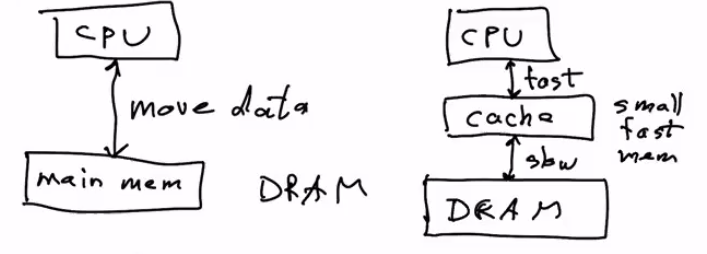
\includegraphics[width=8cm]{images/lec4-1.png}
    \caption{Simple models of sequential and parallel computers}
\end{figure}

For example, on a sequential computer, the main cost of a naive algorithm would be moving data between main memory (DRAM) and on-chip cache, 
and on a parallel computer, it is moving data\footnote{All forms of "moving data" are called "communication"} between processors connected over a network.
We seek to minimize it if possible.

\begin{figure}[h]
    \centering
    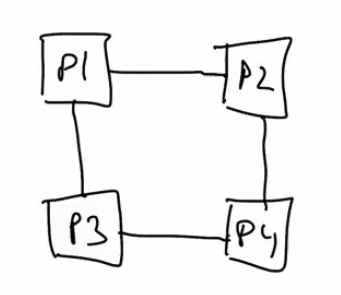
\includegraphics[width=5cm]{images/lec4-2.png}
    \caption{Moving data from $p_i$ to $p_j$ is slow}
\end{figure}

In the case of matrix multiplication, there is a theorem that gives a lower bound on the amount of communication required
between DRAM and cache, assuming one can do the usual $O(n^3)$ operations in any order.  And there is a well-known and widely-used algorithm that attains this lower bound.
In 2011 we showed that this lower bound extends to any algorithm that "smells like" the 3-nested loops of conventional matrix multiplication,
essentially covering all the usual linear algebra algorithms, for solving $Ax=b$, least squares, etc. (\href{http://www.eecs.berkeley.edu/Pubs/TechRpts/2011/EECS-2011-15.html}{"Minimizing Communication in Numerical Linear Algebra"})
It turns out that the usual algorithms for these problem cannot always attain the lower bound, just by doing the same operations in a different order; 
instead one needs new algorithms. Some of these recently invented algorithms have given very large speedups ($O(\times)$) and are widely used.

All these results (lower bounds and optimal algorithms) extend to other kinds of computer architectures, so with multiple layers of cache 
(so there is communication between every pair of of adjacent layers), and with parallel processors 
(so there is communication between different processors over a network).
In this lecture we will talk about this lower bound and optimal algorithm for matrix multiplication, in the simplest case of having DRAM and cache.
In later lectures, when we talk about more complicated linear algebra algorithms, we will just sketch how to redesign them to minimize communication. 

There are many more algorithms, and computer architectures, to which these ideas could be applied, which are possible class projects.
To get started, we want a simple mathematical model of what it costs to move data, so we can analyze algorithms easily and identify the one that is fastest. 
So we need to define two terms: bandwidth and latency.

First, to establish intuition, consider the time it takes to move cars on the freeway from Berkeley to Sacramento:
Bandwidth measures how many cars/hour can get from Berkeley to Sacramento:
\begin{align*}
    \#\mathrm{cars}/\mathrm{hour} = \mathrm{density} (\#\mathrm{cars}/\mathrm{mile}/\mathrm{lane}) \cdot \mathrm{velocity}(\mathrm{miles}/\mathrm{hour}) \cdot \#\mathrm{lanes}
\end{align*}
Latency measures how long it takes for one car to get get from Berkeley to Sacramento:
\begin{align*}
    \mathrm{time} = \mathrm{distance} / \mathrm{velocity}
\end{align*}
So the minimum time it takes $n$ cars to go from Berkeley to Sacramento is when they all travel in a single "convoy", 
which is all as close together as possible given the density, and using all lanes:
\begin{align*}
    \mathrm{time} = \mathrm{time} \text{ for first car to arrive} + \mathrm{time} \text{ for remaining cars to arrive} = \mathrm{latency} + n/\mathrm{bandwidth}
\end{align*}
The same idea (harder to explain the physics) applies to reading bits from main memory to cache: The data resides in main memory initially, 
but one can only perform arithmetic and other operations on it after moving it to the much smaller cache. 
The time to read or write w words of data from memory stored in contiguous locations (which we call a "message" instead of a convoy) is
\begin{align*}
    \mathrm{time} = \mathrm{latency} + w / \mathrm{bandwidth}
\end{align*}
More generally, to read or write $w$ words stored in $m$ separate contiguous messages costs $m \cdot \mathrm{latency} + w / \mathrm{bandwidth}$.
Notation: We will write this cost as $m\alpha + w\beta$, and refer to it as the cost of "communication".
We refer to $w$ as $\#words\_moved$ and $m$ as $\#messages$. We also let $\gamma = \text{time per flop}$, so if an algorithm does $f$ flops,
our estimate of the total running time will be: \begin{align*}
    \mathrm{time} = m\alpha + w\beta + f\gamma
\end{align*}
To reiterate our claim that communication is the most expensive operation:\begin{enumerate}
    \item $\gamma \ll \beta \ll \alpha$ on modern machines (factors of 10s or 100s for memory, even bigger for disk or sending messages between processors)
    \item Gaps are increasing year over year, $\gamma$ faster than $\beta$ faster than $\alpha$
\end{enumerate}

\begin{figure}[h]
    \centering
    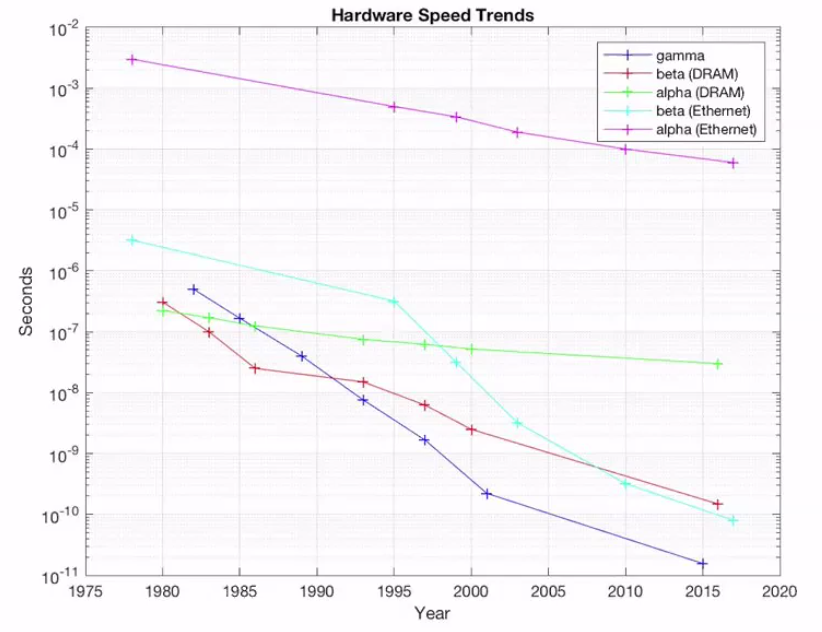
\includegraphics[width = 10cm]{images/lec4-3.png}
    \caption{Hardware speed trends}
\end{figure}

And the same story holds for energy: the energy cost of moving data is much higher than doing arithmetic. So whether you are concerned about the battery in your cell phone dying, 
the O(\$1M) per megawatt per year it takes to run your data center, or how long your drone can stay airborne, you should minimize communication.
So when we design or choose algorithms, we need to pay attention to their communication costs. 

How do we tell if we have designed the algorithm well with respect to not communicating too much? If the $f\gamma$ term in the time dominates the communication cost $m\alpha + w\beta$:
\begin{align*}
    f\gamma \geq m\alpha + w\beta
\end{align*}
then the algorithm is at most 2 times slower than as though communication were free. When $f\gamma \gg m\alpha + w\beta$, 
the algorithm is running at near peak arithmetic speed, and can't go faster. When $f\gamma \ll m\alpha + w\beta$, communication costs dominate.
Note that the Computational Intensity is $q = f/w$, "flops per word moved". This needs to be large to go fast, since $f\gamma > w\beta$ means $q = f/w > \beta/\gamma \gg 1$.

\subsection{Some History}
\subsubsection{The Beginning and \textit{EISPACK}}
We will know we have done as well as possible if we can show that $w$ and $m$ are close to known lower bounds, that we will describe below.
But first to describe how this trend has impacted algorithms over time, we give a little history. In the beginning, was the do-loop. 
This was enough for the first libraries (\textit{EISPACK}, for eigenvalues of dense matrices, in the mid 1960s). People didn't worry about data motion, 
arithmetic was more expensive, they mostly just tried to get answer reliably, for $O(n^3)$ flops.

\subsubsection{\textit{BLAS-1} library (mid 1970s)}
\textit{BLAS-1}\footnote{Basic Linear Algebra Subroutines} was a standard library of 15 operations (mostly) on vectors, including:\begin{enumerate}
    \item $y = \alpha x + y$, $x$ and $y$ vectors, $\alpha$ scalar (\textit{AXPY}) 
    \begin{algorithmfrm}[Example: innermost loop in Gaussian Elimination]
        \begin{algorithmic}[1]
            \For{\texttt{$k=i+1:n$}}
                    \State $A_{jk} = A_{jk} - A_{ji}A_{ik}$
                    \EndFor
        \end{algorithmic}
    \end{algorithmfrm}
    \item Dot product
    \item $\norm{x}_2 = \sqrt{\sum_i x_i^2}$
    \item Find largest entry in absolute value in a vector (for pivoting in Gaussian Elimination)
\end{enumerate}

The motivations for the \textit{BLAS-1} at the time were: \begin{itemize}
    \item easing programming
    \item readability, since these were commonly used functions
    \item robustness (e.g. avoid $\mathrm{over}/\mathrm{underflow}$ in $\norm{x}_2$)
    \item portable and efficient (if optimized on each architecture)
\end{itemize}
But there is no way to minimize communication in such simple operations, because they do only a few flops per memory reference,
e.g. $2n$ flops on $2n$ data for a dot product, so with a computational intensity of $q=\frac{2n}{2n}=1$. 
So if we implement matrix multiplication or Gaussian Elimination or anything else by loops calling \textit{AXPY}, it will communicate a lot, 
the same as the number of flops.

\subsubsection{\textit{BLAS-2} library (mid 1980s)}
This was a standard library of 25 operations (mostly) on matrix-vector pairs:\begin{enumerate}
    \item $y=\alpha y+\beta A x$ (\textit{GEMV}\footnote{General matrix vector multiply}), with lots of variations for different matrix structures (symmetric, banded, triangular etc.) It allowed did obvious optimizations when $\alpha$ and/or $\beta = \pm 1,0$
    \item $A=A+\alpha xy^\top$ (\textit{GER}\footnote{General rank one update}). It turns out the 2 innermost loops in GE can be written with GER (details later): \begin{align*}
        A(i+1:n,i+1:n) = A(i+1:n,i+1:n) - A(i+1:n,i) A(i,i+1:n)
    \end{align*}
    \item Solve $Tx=b$ where $T$ triangular (used by Gaussian Elimination to solve $Ax=b$) (\textit{TRSV}). The motivation was similar to the \textit{BLAS-1}, plus more opportunities to optimize on the vector computers of the day. But there is still not much reduction in communication, 
    for example, \textit{GEMV} reads $n^2+2n+2$ words, writes $n$ words, and does $2n^2+3n$ flops, for a computational intensity of about $q=2$.
\end{enumerate}

\subsubsection{\textit{BLAS-3} library (late 1980s)}
This was a standard library of 9 operations on matrix-matrix pairs: \begin{enumerate}
    \item $C=\beta C+\alpha AB$ (\textit{GEMM}\footnote{General matrix-matrix multiply})
    \item $C=\beta C+\alpha AA^\top$ (\textit{SYRK}\footnote{Symmetric rank update})
    \item Solve $TX=B$ where $T$ triangular, $X$ and $B$ are rectangular matrices (\textit{TRSM})
\end{enumerate}
Finally these have the potential for significant communication optimization, since for example the computational intensity $q$ of \textit{GEMM} applied to $n \times n$ matrices is: \begin{align*}
    q = \frac{f}{w} = \frac{2n^3}{3n^2 \mathrm{input} + n^2 \mathrm{output}} = \frac{n}{2}
\end{align*}
But as we'll see, the straightforward 3-nested-loop version of \textit{GEMM} is no better than \textit{BLAS-2} or \textit{BLAS-1}, 
so a different implementation is required, with very large speedups possible. In fact, there is an optimal way to implement \textit{GEMM}, 
that provably does as little communication as possible (under certain assumptions).
Note: \href{www.netlib.org/blas}{\textit{BLAS-k}} does $O(n^k)$ operations, for $k=1,2,3$, making the names easier to remember. These are supplied as part of the optimized math libraries on essentially all computers.
 
This led the community to seek algorithms for the rest of linear algebra (solving $Ax=b$, least squares, computing eigenvalues, SVD, etc.)
that did much of their work by calling BLAS-3 routines, which would then run at high speed. This led to the \textit{LAPACK} library 
(and its parallel version called \textit{ScaLAPACK}) which is the basis of most dense linear algebra libraries provided by computer vendors, 
and used in many packages like \textit{MATLAB}.

As stated earlier, we later discovered that the communication lower bounds attained by \textit{GEMM} also apply to essentially the rest of linear algebra. 
Next we realized that the algorithms in \textit{LAPACK} and \textit{ScaLAPACK} usually did not attain these lower bounds, 
in fact the algorithms there could do asymptotically more communication than the bounds required. This in turn set off a search for new 
(or previously invented but ignored) algorithms that would attain these lower bounds. This has led to a number of new algorithms, some with large speedups ($O(10\times)$),
and some still of just theoretical interest.

\subsection{Analysis on Matrix multiplication}
\textbf{Goals}: Prove communication lower bound for matrix multiplication

\begin{figure}[h]
    \centering
    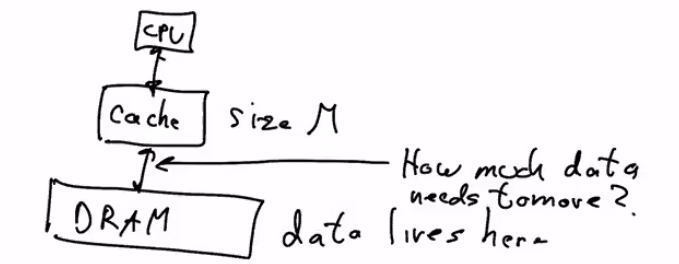
\includegraphics[width = 7cm]{images/lec4-4.png}
    \caption{The goal}
\end{figure}

The following theorem for matrix multiplication was first proved in 1981 by Hong and Kung. The proof below is based on one by Irony, Tiskin and Toledo in 2004, 
which extends both to parallel algorithms, and to other 3-nested-loop-like algorithms.

\begin{theorem}
    Suppose one wants to multiply two nxn matrices $C = AB$ by doing the usual $2n^3$ multiplies and adds, 
    on a computer with a main memory large enough to hold $A$, $B$ and $C$, and a smaller cache of size $M$. Arithmetic can only be done on data stored in cache. 
    Then a lower bound on the number of words $W$ that need to move back and forth between main memory and cache to run the algorithm is \begin{align*}
        \Omega(\frac{n^3}{\sqrt{M}})
    \end{align*}
\end{theorem}

More generally, one does not need to multiply dense square matrices, the same proof works for rectangular and/or sparse matrices; 
the only change is that $\Omega(n^3/\sqrt{M})$ becomes $\Omega(\#\mathrm{flops}/sqrt{M})$.

\begin{proof}[Proof Sketch]
    Suppose we fill up the cache with M words of data, do as many flops as possible, store the results back in main memory,
    and repeat until we are done. Suppose we could upper bound by $G$ the number of flops that are possible given M words of data. 
    Then doing $G$ flops would cost at least $2M$ words moved back and forth between main memory and cache. Since we have to do $2n^3$ flops altogether,
    we would need to repeat this at least $2n^3/G$ times, for a total cost of moving at least $(2n^3/G)2M$ words. So we need to find an upper bound $G$.

    \begin{figure}[h]
        \centering
        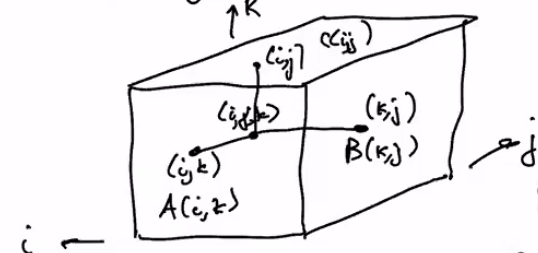
\includegraphics[width=7cm]{images/lec4-5.png}
        \caption{The geometry problem}
    \end{figure}
    
    We turn this into a geometry problem as follows. We represent each pair of flops (or inner loop iteration) \begin{align*}
        C(i,j) = C(i,j) + A(i,k)B(k,j)
    \end{align*}
    as a lattice point $(i,j,k)$ in 3D space, with $1 \leq i,j,k \leq n$, so an $n \times n \times n$ cube of points. 
    The flops we can do with $M$ words of data is represented by some subset $V$ of this cube of lattice points.
    What data is required to execute the flops represented by $(i,j,k)$? It is $C(i,j)$, $A(i,k)$, and $B(k,j)$, 
    which are represented by the 3 lattice points $(i,j)$, $(i,j)$ and $(k,j)$ on 3 faces of the cube, i.e. the projections of $(i,j,k)$ onto these three faces.
    We know we can have at most M words of data, i.e. $M$ projected points. We now use a classical geometry theorem by Loomis and Whitney (1949),
    which says that if the set of lattice points is $V$ whose cardinality $|V|$ we want to bound, and its 3 projections onto the faces of the cube are \begin{itemize}
        \item $V_C$ (representing entries $C(i,j)$)
        \item $V_A$ (representing entries $A(i,k)$)
        \item $V_B$ (representing entries $B(k,j)$)
    \end{itemize}
    then $|V| \leq \sqrt{|V_A| |V_B| |V_C| }$. Since we can have at most $M$ entries of $A$, $B$ and $C$ in cache, this means \begin{align*}
        |V| \leq \sqrt{M \cdots M \cdots M} = M^{3/2}
    \end{align*}
    yielding our desired upper bound $G = M^{3/2}$. Finally, this yield our lower bound $W \geq (2*n^3)/M^{3/2} 2M = \Omega(n^3/\sqrt{M})$ as claimed.
    We have not tried to be careful with the constant factors, but just tried to give the main idea. The best (nearly attainable) lower bound is actually $2 n^3/\sqrt{M} - 2M$.
    \begin{figure}[h]
        \centering
        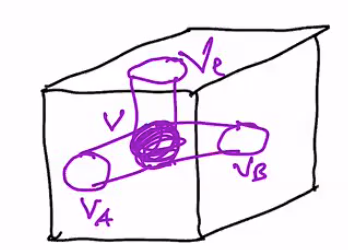
\includegraphics[width=7cm]{images/lec4-6.png}
        \caption{$V_A$, $V_B$ and $V_C$}
    \end{figure}
\end{proof}

The proof also gives us a big hint as to how to design an optimal algorithm: What is the shape of the $V$ that attains its upper bound $M^{3/2}$? 
Clearly $V$ must be a cube of side length $\sqrt{M}$. This means that we will want to break $A$, $B$ and $C$ up into square submatrices of dimension at most $\sqrt{M/3}$, 
read 3 submatrices into cache (the factor of 3 means we can fit 3 such submatrices simultaneously), multiply them, and write the results back to main memory.

\begin{algorithmfrm}
    \begin{algorithmic}[1]
        \State Let $b$ be block size, small enough so $3b^2\leq M$
        \State Express $C$ as a block matrix where $C[i,j]$ is a $b \times b$ block 
        \For{\texttt{$i=1:n/b$}}
            \For{\texttt{$j=1:n/b$}}
                \State read $C[i,j]$ into cache \Comment{$b^2$ words moved}
                \For{\texttt{$k=1:n/b$}}
                    \State read $A[i,k]$ and $B[k,j]$ into cache \Comment{$2b^2$ words moved}
                    \State $C[i,j] = C[i,j] + A[i,k]B[k,j]$ \Comment{$b \times b$ matrix multiplication, so 3 more nested loops}
                \EndFor
                \State write $C[i,j]$ back to main memory \Comment{$b^2$ words moved}
            \EndFor
        \EndFor
    \end{algorithmic}
\end{algorithmfrm}

\begin{figure}[h]
    \centering
    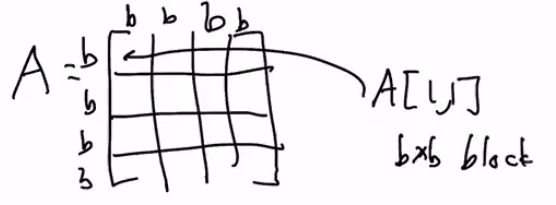
\includegraphics[width=7cm]{images/lec4-7.png}
    \caption{$A$ into blocks}
\end{figure}

Counting the total number of words moved between cache and memory, we get \begin{align*}
    \begin{array}{ll}
        \text{For reading } C[i,j] & (n/b)^2 b^2 = n^2 \\
        \text{For reading } A[i,k] \text{ and } B[k,j] & (n/b)^2 b^2 = n^2 \\
        \text{For writing } C[i,j] & (n/b)^2 b^2 = n^2
    \end{array}
\end{align*}
for a total of $2 n^3/b + 2n^2$ words moved. We minimize this by making $b$ as large as possible, i.e. $b = \sqrt{\frac{M}{3}}$, 
or the number of words moved = $O(n^3/\sqrt{M})$, which attains the lower bound (to within a constant factor).

What about "What about multiplying a $A \times B$ where $B$ has just a few columns, or just one?" It is still 3 nested loops,
but if $B$ has fewer than $b$ columns, then we can't break it into $b \times b$ blocks. 
But all the above lower bounds and optimal algorithms can be extended to the case of small loop bounds; the (attainable) lower bound becomes \begin{align*}
    \Omega (\max (\frac{\#\mathrm{flops}}{\sqrt{M}}, \operatorname{size}(\mathrm{input}), \operatorname{size}(\mathrm{output})))
\end{align*}
This approach to finding a communication lower bound and corresponding optimal algorithm has recently been extended to any algorithm that
can be expressed as nested loops accessing arrays, with any number of loops, arrays, and subscripts, as long as the subscripts are "affine". 
The lower bound is always of the form: \begin{align*}
    \Omega(\frac{\#\mathrm{loop iterations}}{M^e}),
\end{align*}
 where $e$ is an exponent that depends on the problem ($e=1/2$ for matrix multiplication). And the optimal block shapes can be general parallelograms.
For linear algebra, we only need the special case described above. Here is another optimal matrix multiplication algorithm, 
that we will find simpler to generalize to other linear algebra problems, because it is "cache oblivious", i.e. it works for any cache size $M$, 
without needing to know $M$:

\begin{savenotes}
    \begin{algorithmfrm}[Cache Oblivious]
        \begin{algorithmic}[1]
            \State Function $C = \operatorname{RMM}(A,B)$\footnote{Recursive Matrix Multiplication}\footnote{Assume for simplicity that $A$ and $B$ are square of size $n$}\footnote{Assume for simplicity that $n$ is a power of 2}
            \State Express $C$ as a block matrix where $C[i,j]$ is a $b \times b$ block 
            \If{\texttt{$n=1$}}
                \State $C=AB$
            \Else 
                \State write $A=\left[\begin{array}{ll}
                    A_{11} & A_{12} \\
                    A_{21} & A_{22}
                    \end{array}\right]$ where each $A_{ij}$ is $\frac{n}{2} \times \frac{n}{2}$
                \State write $B$ and $C$ similarly
                \State $C_{11} = \mathbf{RMM}(A_{11},B_{11}) + \mathbf{RMM}(A_{12},B_{21})$
                \State $C_{12} = \mathbf{RMM}(A_{11},B_{12}) + \mathbf{RMM}(A_{12},B_{22})$
                \State $C_{21} = \mathbf{RMM}(A_{21},B_{11}) + \mathbf{RMM}(A_{22},B_{21})$
                \State $C_{22} = \mathbf{RMM}(A_{21},B_{12}) + \mathbf{RMM}(A_{22},B_{22})$
            \EndIf 
        \end{algorithmic}
    \end{algorithmfrm}
\end{savenotes}

Cost: let $A(n)$ be the number of arithmetic operation on matrices of dimension $n$, \begin{align*}
    A(n) = 8A(\frac{n}{2}) + n^2
\end{align*}
Claim that $A(n) = 2n^3 - n^2$, same as the classical algorithm. Solve by changing variables from $n=2^m$ to $m$ \begin{align*}
    a(m) = 8a(m-1) + 2^{2m}
\end{align*}
Divide by $8^m$ to get \begin{align*}
    \frac{a(m)}{8^{m}}=\frac{a(m-1)}{8^{m-1}}+2^{-m}
\end{align*}
Change variables again to $b(m) = a(m)/8^m$,\begin{align*}
    b(m) &= b(m-1)+2^{-m} \\
    &= \sum_{k=1}^{m} 2^{-k}+b(0)
\end{align*}

Let $W(n)$ be the number of words moved between slow memory and cache of size $M$,\begin{align*}
    W(n) &= 8  w\left(\frac{n}{2}\right) + 12\left(\frac{n}{2}\right)^{2} \\
    &= 8  w\left(\frac{n}{2}\right) + 3n^2
\end{align*}
which looks bigger than $A(n)$. The base case is not at $W(1)$, rather \begin{align*}
    w(b)=3 b^{2}
\end{align*}
if $3b^{2} \leq M$, i.e. $b=\sqrt{\frac{M}{3}}$. Solve as before: change variables from $n=2^m$ to $m$: \begin{align*}
    w(m)=8 w(m-1)+3 \cdot 2^{2 m}
\end{align*}
Let $\bar{m} = \log_2 \sqrt{\frac{M}{3}}$. Divide by $8^m$ to get $v(m) = w(m)/8^m$: \begin{align*}
    v(m) &=v(m-1)+3 \cdot(1 / 2)^{n} \\
    v(\bar{m})=M / 8^{\bar{m}}=M /(M / 3)^{3 / 2}=3^{3 / 2} / M^{1 / 2}
\end{align*}
This is again a geometric sum but just down to $m = \bar{m}$, not 1: \begin{align*}
    v(m) &= \sum_{k=\bar{m}+1}^{m} 3(1 / 2)^{k}+v(\bar{m}) \\
    &\leq 2 \cdot 3^{3 / 2} / \sqrt{M}
\end{align*}
So \begin{align*}
    W(n) = w(\log_2 n) = 8^{\log_2 n} v(\log_2 n) = 2 \cdot 3^{3/2} \frac{n^3}{\sqrt{M}}
\end{align*}
as desired.

We mention briefly that the lower bound extends to the parallel case in a natural way: now the "cache" is the memory local to each processor, that it can access quickly, 
and "main memory" is the memory local to all the other processors, which is much slower to access. We assume each processor is assigned an equal fraction of the flops to do, 
$2 \frac{n^3}{P}$, where $P$ is the number of processors, and an equal fraction of the memory required to store all the data, so $M = 3 \frac{n^2}{P}$. 
Then the same proof as above says that for each processor to perform $2 \frac{n^3}{P}$ flops it needs to move
\begin{align*}
    \Omega((n^3/P)/\sqrt{M}) = \Omega(n^2/\sqrt{P})
\end{align*}
words into and out of its local memory. This lower bound is indeed attained by known algorithms, such as \textit{SUMMA}\footnote{Scalable Universal Matrix Multiply Algorithm}.

\subsection{The Strassen Algorithm}

We can go asymptotically faster than $n^3$, not just to multiply matrices, but any linear algebra problem. There are many such algorithms,
we discuss only the first one, which so far is the most practical one.

Matrix multiply is possible in $O(n^(\log_2 7)) \sim O(n^{2.81})$ operations. The algorithm is recursive, based on remarkable identities for multiplying $2 \times 2$ matrices.

Write $A=\left[\begin{array}{ll}
    A_{11} & A_{12} \\
    A_{21} & A_{22}
    \end{array}\right]$ where each $A_{ij}$ is $\frac{n}{2} \times \frac{n}{2}$, same for $B$ and $C$.\\
$P_1 = (A_{12}-A_{22})(B_{21}+B_{22})$,\\
$P_2 = (A_{11}+A_{22})(B_{11}+B_{22})$,\\
$P_3 = (A_{11}-A_{21})(B_{11}+B_{12})$,\\
$P_4 = (A_{11}+A_{12})B_{22}$,\\
$P_5 = A_{11}(B_{12}-B_{22})$,\\
$P_6 = A_{22}(B_{21}-B_{11})$,\\
$P_7 = (A_{21}+A_{22})B_{11}$,\\
$C_11 = P_1+P_2-P_4+P_6$,\\
$C_12 = P_4+P_5$,\\
$C_21 = P_6+P_7$,\\
$C_22 = P_2-P_3+P_5-P_7$

\begin{savenotes}
    \begin{algorithmfrm}[Strassen algorithm]
        \begin{algorithmic}[1]
            \State Function $C = \operatorname{Strassen}(A,B)$\footnote{Recursive Matrix Multiplication}\footnote{Assume for simplicity that $A$ and $B$ are square of size $n$}\footnote{Assume for simplicity that $n$ is a power of 2}
            \State Express $C$ as a block matrix where $C[i,j]$ is a $b \times b$ block 
            \If{\texttt{$n=1$}}
                \State $C=AB$
            \Else 
                \State $P_1=\operatorname{Strassen}(A_{11}-A_{22}, B_{21}+B_{22})$ \Comment{And 6 more similar lines}
                \State $C_{11}=P_1+P_2-P_4+P_6$ \Comment{And 3 more similar lines}
            \EndIf 
        \end{algorithmic}
    \end{algorithmfrm}
\end{savenotes}

The arithmetic operations \begin{align*}
    A(n) = 7 A\left(\frac{n}{2}\right)+18\left(\frac{n}{2}\right)^{2}
\end{align*}

We solve as before: change variables from $n=2^m$ to $m$, $A(n)$ to $a(m)$:\begin{align*}
    a(m) = 7a(m-1) + (9/2)2^(2m)
\end{align*}
Divide by $7^m$, change again to $b(m) = a(m)/7^m$, \begin{align*}
    b(m) = b(m-1) + (9/2) \cdot (4/7)^m
\end{align*}
So \begin{align*}
    A(n) = a\left(\log_{2} n\right) = b\left(\log_{2} n\right)*7^{\log_{2} n} = O(7^{\log_{2} n}) = O(n^{\log_{2} 7})
\end{align*} 
 About the number of words moved, again get a similar recurrence: \begin{align*}
    W(n) = 7W(n/2) + O(n^2),
 \end{align*}
and the base case $W(\bar{n}) = O(\bar{n}^2)$ when $\bar{n}^2 = O(M)$, i.e. the whole problem fits in cache.
The solution is $O(n^x/M^{x/2 -1})$ where $x = log_2 7$.
Note that plugging in $x=3$ gives the lower bound for standard matrix multiplication. Again, there is a theorem (with a very different proof), 
showing that this algorithm is optimal:
\begin{theorem}[Demmel, Ballard, Holtz, Schwartz, 2010]
    $\Omega(n^x/M^{x/2 - 1})$ is a lower bound on $\#\mathrm{words\_moved}$ for \textit{Strassen} and algorithms "enough like" Strassen, where $x = \log_2 7$ for \textit{Strassen}, and whatever it is for "Strassen-like" methods.
\end{theorem}

This result was generalized to even more "Strassen-like" methods in a PhD Thesis (Scott, 2015). Strassen is not (yet) much used in practice, but it can pay off for $n$ not too large (a few hundred).
The current world's record is by Le Gall (2014): $O(n^{2.3728639})$, but it is impractical: would need huge $n$ to pay off.

Its error analysis slightly worse than usual algorithm: Usual matrix multiplication: \begin{align*}
    |\operatorname{fl}(AB) - (AB)| \leq n \varepsilon|A||B|
\end{align*}
For \textit{Strassen}: \begin{align*}
    \|\operatorname{fl}(AB) - (AB)\| \leq O(\varepsilon) |A||B|
\end{align*} which is good enough for lots of purposes. But when can \textit{Strassen}'s error bound be much worse?
(suppose one row of A, or one column of B, is very tiny).
\textit{Strassen} is also not allowed to be used in the \href{www.top500.org}{"LINPACK Benchmark"} which ranks machines by \begin{align*}
    \mathrm{speed} = (2/3)n^3 / \operatorname{time\_for\_GEPP}(n).
\end{align*}
And if you use \textit{Strassen} in \textit{GEPP}, it does far smaller than $(2/3)n^3$ flops so the computed "speed" could exceed actually peak machine speed. 
As a result, vendors stopped optimizing \textit{Strassen}, even though it's a good idea!

A similar Strassen-like trick can be used to make complex matrix multiplication a constant factor cheaper than you think. Normally,
to multiply two complex numbers or matrices, you use the formula \begin{align*}
    (A+iB)(C+iD) = (AC-BD)+i(AD+BC)
\end{align*}
costing 4 real multiplications and 2 real additions. Here is another way:
$T1 = AC$,\\
$T2 = BD$,\\
$T3 = (A+B)(C+D)$.\\
Then it turns out that \begin{align*}
    (A+iB)(C+iD) = (T_1 - T_2) + i(T_3 - T_1 - T_2)
\end{align*}
for a cost of 3 real multiplications and 5 real additions. But since matrix multiplication costs $O(n^3)$ or $O(n^x)$ for some $x>2$,
and addition costs $O(n^2)$, for large $n$ the cost drops by a factor $3/4$. The error analysis is very similar to the usual algorithm.
Applying the above formula recursively in a different context yields an algorithm for multiplying two $n$-bit integers in
$O(n^{\log_2 3}) = O(n^{1.59})$ bit operations, as opposed to the conventional $O(n^2)$.

\newpage
\section{Lecture 5: Gaussian Elimination}
\subsection{Gaussian Elimination}
Exploit Structure:A symmetric, positive definite "sparse" depends on $\ll n^2$ parameters, so could have lots of zero entries, or be dense but depend on few parameters, e.g. Vandermonde.

Seek Matrix Factorizations: $A=$ product of simple matrices
\begin{itemize}
    \item $A=U \Sigma V^{\top}=\text{orthogonal}\cdot\text{diagonal}\cdot \text{orthogonal}$
    \item Gaussian Elimination: $A=PL U$ 
    \item For solving $Ax=b$, Least Squares: $A=Q  R$, $Q$ orthogonal, $R$ upper triangular
    \item eigenproblems: $A=QTQ^H$, $Q$ unitary, $T$ upper triangular
\end{itemize}

\begin{definition}[permutation Matrix]
    Identity matrix with permuted rows.
\end{definition}

\begin{fact}
    To store and multiply by $P$ requires store locations of $1$ (cheap)
    \begin{enumerate}
        \item $P,P_1, P_2$ permutation matrices. $P$ has exactly one $1$ in each row and each column.
        \item $P X = X$ with permuted rows
        \item $X P = X$ with permuted columns
        \item $P_1  P_2 = \text{permutation}$ 
        \item $P^{-1}=P^{\top}$ i.e. $P$ orthogonal (check: $P P^{\top}$ has unit diagonal)
        \item $\operatorname{det}(P) = \pm 1$
    \end{enumerate}
\end{fact}

\begin{savenotes}
    \begin{theorem}[LU Decomposition]
        Given any $m \times n$ full rank $A$, $m \geq n$, $\exists \ m \times m \text{ permutation } P, \ \ m \times n $ unit lower triangular $L, \ n \times n \text{ nonsingular upper triangular }U$
        such that $A=PL U$.
        \begin{proof}
            If $A$ is full rank, the first column is nonzero, so there is a permutation $P$ such that $(PA)_{11}$ is nonzero. Write \begin{align*}
                PA &= \left[\begin{array}{ll}
                    A_{11} & A_{12} \\
                    A_{21} & A_{22}
                    \end{array}\right] \\
                &= \left[\begin{array}{ll}
                    1 & 0 \\
                    \frac{A_{21}}{A_{11}} & I
                    \end{array}\right] \left[\begin{array}{ll}
                        A_{11} & A_{12} \\
                        0 & A_{22} - \frac{A_{21} A_{12}}{A_{11}}
                        \end{array}\right]
            \end{align*}
            where $A_{11}$ is $1 \times 1$, $A_{21}$ is $(m-1) \times 1$, $A_{12}$ is $1 \times (n-1)$ and $A_{22}$ is $(m-1) \times (n-1)$.
            Now $A$ full (column) rank $\Longrightarrow$ $PA$ full rank $\Longrightarrow$ $S = A_{22} - \frac{A_{21} A_{12}}{A_{11}}$ is full rank\footnote{$S$ is the Schur complement}. 
            (Otherwise, if some nonzero linear combination of columns of $S$ were 0, say $Sx=0$, then a linear combination of columns of $A$ would be zero, 
            $A\left[ -A_{12} x/A_{11} ; x \right] = 0$, contradicting $A$ being full column rank. More simply in the square case: \begin{align*}
                0 &= \operatorname{det}(A) = \pm \operatorname{det}(PA) = \operatorname{det}(\text{first factor}) \cdot \operatorname{det}(\text{second factor}) \\
                &= 1 \cdot A_{11} \cdot \operatorname{det}(S) \\
                &\Longrightarrow \operatorname{det}(S) \neq 0
            \end{align*}
            Now apply induction: $S = P^\prime L^\prime U^\prime$, so \begin{align*}
                PA &= \left[\begin{array}{ll}
                    1 & 0 \\
                    \frac{A_{21}}{A_{11}} & I
                    \end{array}\right] \left[\begin{array}{cc}
                        A_{11} & A_{12} \\
                        0 & P^{\prime} L^{\prime} U^{\prime}
                        \end{array}\right] \\
                &= \left[\begin{array}{ll}
                    1 & 0 \\
                    \frac{A_{21}}{A_{11}} & P^{\prime} L^{\prime}
                    \end{array}\right] \left[\begin{array}{cc}
                        A_{11} & A_{12} \\
                        0 &  U^{\prime}
                        \end{array}\right] \\
                &= \left[\begin{array}{ll}
                    1 & 0 \\
                    0 & P^{\prime}
                    \end{array}\right] \left[\begin{array}{cc}
                        1 & 0 \\
                        P^{\prime \top}\frac{A_{21}}{A_{11}} &  L^{\prime}
                        \end{array}\right]\left[\begin{array}{cc}
                            A_{11} & A_{12} \\
                            0 &  U^{\prime}
                            \end{array}\right]
            \end{align*}
            \begin{align*}
                A = P^\top \left[\begin{array}{ll}
                    1 & 0 \\
                    0 & P^{\prime}
                    \end{array}\right] \left[\begin{array}{cc}
                        1 & 0 \\
                        P^{\prime \top}\frac{A_{21}}{A_{11}} &  L^{\prime}
                        \end{array}\right]\left[\begin{array}{cc}
                            A_{11} & A_{12} \\
                            0 &  U^{\prime}
                            \end{array}\right]
            \end{align*} where the 3 matrices are permutation, unit lower triangular and upper triangular respectively.
        \end{proof}
    \end{theorem}
\end{savenotes}



\begin{corollary}
    If A $n \times n$ and nonsingular, there exist an $n \times n$ permutation $P$, unit lower triangular $L$, 
    and nonsingular upper triangular $U$ such that $A = PLU$
\end{corollary}

To solve $Ax=b$:
\begin{enumerate}
    \item factor: $A=PL U$ (expensive part, $\text{cost}=\frac{2}{3}n^3+O(n^2)$)
    \item Solve $ P LU x = P^{\top} b$ for $LUx=P^{\top}b$ by permuting $b$, $\text{cost}=O(n)$
    \item Solve $ LU x = P^{\top} b$ for $Ux=L^{-1}P^{\top}b$ by forward substitution with $L$, $\text{cost}=n^2$
    \item Solve $Ux=L^{-1}P^{\top}b$ for $x=U^{-1} L^{-1}P^{\top}b=A^{-1}b$ using back substitution with $U$, $\text{cost}=n^2$
\end{enumerate}
If we are given another $b'$, can solve $Ax^\prime=b^\prime$ in just $O(n^2)$ flops.

Note: We do not compute $A^{-1}$ and multiply $x=A^{-1} b$ because
\begin{enumerate}
    \item Three times more expensive in dense case (can be $O(n^2)$ more expensive in sparse case)
    \item Not as numerically stable
\end{enumerate}

How to pivot, i.e. choose $A_{ii}$ to put on diagonal, goal being back stability:
$$P L U=A+E, \ \|E\|=O(\varepsilon)\|A\|$$
This not guaranteed by $A_{ii} \neq 0$.

\subsection{Gaussian Elimination in Algorithm}
\begin{algorithmfrm}
    \begin{algorithmic}[1]
        \For{\texttt{$i=1:n$}}
            \If{\texttt{$i=1$}}
                \State Performs algebra shown above,
            \Else \If{\texttt{$i>1$}}
                    \State Applies the same algorithm recursively to the Schur complement
                \EndIf
            \EndIf 
            \State $L(i,i)=1$
            \State $L(i+1:n,i) = A(i+1:n,i)/A(i,i)$ \Comment{Ignore permutations for now}
            \State $U(i,i:n) = A(i,i:n)$
            \If{\texttt{$i=1$}}
                \State $A(i+1:n,i+1:n) = A(i+1:n,i+1:n) - L(i+1:n,i) U(i,i+1:n)$
            \EndIf
        \EndFor
    \end{algorithmic}
\end{algorithmfrm}

Add permutations after the first "for loop", add:
\begin{algorithmfrm}
    \begin{algorithmic}[1]
        \If{\texttt{$ A(i,i) = 0$ and $A(j,i) \neq 0$}}
            \State swap rows $i$ and $j$ of $L$ and $A$; record swap \Comment{How to choose $A(j,i)$ called "pivoting"}
        \EndIf
    \end{algorithmic}
\end{algorithmfrm}

Don't waste space:
row $i$ of $U$ overwrites row $i$ of A: omit $U(i,i:n) = A(i,i:n)$ \\
col $i$ of $L$ (below diagonal) overwrites same entries of $A$, which are zeroed out: change first line to $A(i+1:n,i) = A(i+1:n,i)/A(i,i)$\\
only need to loop from $i = 1$ to $n-1$, and change last line from
$$A(i+1:n,i+1:n) = A(i+1:n,i+1:n) - L(i+1:n,i)U(i,i+1:n)$$
to
$$A(i+1:n,i+1:n) = A(i+1:n,i+1:n) - A(i+1:n,i)*A(i,i+1:n)$$

Finally, we get
\begin{algorithmfrm}
    \begin{algorithmic}[1]
        \For{\texttt{$i=1:n-1$}}
        \If{\texttt{$ A(i,i) = 0$ and $A(j,i) \neq 0$}}
            \State swap rows $i$ and $j$ of $L$ and $A$; record swap
            \State $A(i+1:n,i) = A(i+1:n,i)/A(i,i)$ \Comment{call to \textit{BLAS1} routine \textit{scal}}
            \State $A(i+1:n,i+1:n) = A(i+1:n,i+1:n) - A(i+1:n,i)A(i,i+1:n)$\Comment{call to \textit{BLAS2} routine \textit{GER}}
        \EndIf
        \EndFor
    \end{algorithmic}
\end{algorithmfrm}

\begin{figure}
    \centering
    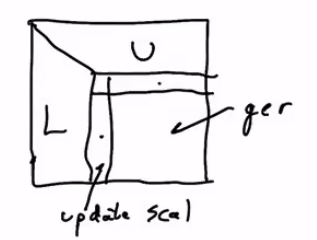
\includegraphics[width=7cm]{images/lec5-1.png}
    \caption{Intermediate step}
\end{figure}

When we're done:\begin{itemize}
    \item $U$ overwrites upper triangle and diagonal of $A$;
    \item $L$ (below diagonal) overwrites $A$ (below diagonal), the unit diagonal entries $L(i,i)=1$ are not stored.
\end{itemize}

To see that this is the same Gaussian Elimination you learned long ago, start from
\begin{algorithmfrm}
    \begin{algorithmic}[1]
        \For{\texttt{$i=1:n-1$}}\Comment{For each column $i$}
            \For{\texttt{$j=i+1:n$}}\Comment{Add a multiple of row $i$ to row $j$ to zero out entry $(j,i)$ below diagonal}
            \State $ m = A(j,i)/A(i,i)$
            \State $ A(j,i:n) = A(j,i:n) - m*A(i,i:n)$
            \EndFor
        \EndFor
    \end{algorithmic}
\end{algorithmfrm}
"Optimize" this by \begin{enumerate}
    \item Not bothering to compute the entries below the diagonal you know are zero: change last line to $A(j,i+1:n) = A(j,i+1:n) - m*A(i,i+1:n)$
    \item Compute all the multipliers $m$ first, store them in zeroed-out locations:\begin{algorithmfrm}
        \begin{algorithmic}[1]
            \For{\texttt{$i=1:n-1$}}
                \For{\texttt{$j=i+1:n$}}
                    \State $A(j,i) = A(j,i)/A(i,i)$
                \EndFor
                \For{\texttt{$j=i+1:n$}}
                    \State $A(j,i+1:n) = A(j,i+1:n) - A(j,i)A(i,i+1:n)$
                \EndFor
            \EndFor
        \end{algorithmic}
    \end{algorithmfrm}
    \item Combine loops into single expressions to get same as before:\begin{algorithmfrm}
        \begin{algorithmic}[1]
            \For{\texttt{$i=1:n-1$}}
                \State $A(i+1:n,i) = A(i+1:n,i)/A(i,i)$
                \State $A(i+1:n,i+1:n) = A(i+1:n,i+1:n) - A(i+1:n,i)A(i,i+1:n)$
            \EndFor
        \end{algorithmic}
    \end{algorithmfrm}
\end{enumerate}
The cost is $\sum_{i=1}^{n-1} 2(n-i)^2 = (2/3)n^3 + O(n^2)$ multiplies and adds.

We need to do pivoting carefully, i.e. choosing which nonzero to put on the diagonal, even if $A(i,i)$ is nonzero, to get a backward stable result, i.e. 
$PLU = A + E$ where $E$ is small compared to $A$. 

\begin{example}[Single Precision]
    If we run in single precision, so with 7 decimal digits, and take \begin{align*}
        A=\left[\begin{array}{cc}
            10^{-8} & 1 \\
            1 & 1
            \end{array}\right], A^{-1} \approxeq \left[\begin{array}{cc}
            -1 & 1 \\
            1 & -10^{-8}
            \end{array}\right]
    \end{align*}
    then $\kappa(A) \sim 2.6$, really small, so we expect a good answer. But \begin{align*}
        L=\left[\begin{array}{ll}
            1 & 0 \\
            10^{8} & 1
            \end{array}\right], U=\left[\begin{array}{ll}
            10^{-8} & 1 \\
            0 & \underbrace{\operatorname{fl}\left(1-10^{8.1}\right)}_{-10^{8}}
            \end{array}\right]
    \end{align*}
    thus \begin{align*}
        L U =\left[\begin{array}{ll}
            10^{-8} & 1 \\
            1 & 0
            \end{array}\right]
    \end{align*}
    which is very different from $A$ in the $(2,2)$ entry. In fact, we'd get the same (wrong) $L$ and $U$ if $A(2,2)$ were $.5$, $-1$, etc. 
    because the operation $\operatorname{fl}(A(2,2)-1\mathrm{e}8*1)$ "forgets" $A(2,2)$ if $A(2,2)$ is small enough, say $O(1)$. 
    So going on to solve $Ax=b$ using $L$ and $U$ will give very wrong answers.

    If we instead pivot (swap rows $1$ and $2$) so $A(1,1)=1$, then we get full accuracy. The intuition is that we want to pick a large entry of $A$ to
    be the "pivot" $A_{11}$, and repeat this at each step, for reasons we formalize below. To motivate the statement of the result, 
    recall HW 1.10, where you showed $C = \operatorname{fl}(AB) = AB + E$ where \begin{align*}
        |E| \leq n \varepsilon |A||B|.
    \end{align*}
    Since $A =PLU$ in exact arithmetic, the following theorem shoule be no surprise.
\end{example}

\begin{theorem}[Backward error analysis of LU decomposition]
    If $P$, $L$ and are computed by the above algorithm, then \begin{align*}
        A - E = PLU
    \end{align*}
    where $|E| \leq n \varepsilon P|L||U|$.
    \begin{proof}
        Recall that for simplicity we assume $P=I$. If we trace through the algorithm and ask how $U(i,j)$ is computed, 
        we see that we start with $A(i,j)$ when $i \leq j$ and repeatedly subtract $L(i,k)U(k,j)$ for $k=1,2,\cdots, i-1$ until we get \begin{align*}
            U(i,j) = A(i,j) - \sum_{k=1}^{i-1} L(i,k)U(k,j)
        \end{align*}
        which, not surprisingly, is what you get when you take the $(i,j)$ entry of $A = LU$ and solve for $U(i,j)$. So $U(i,j)$ is essentially computed by
        a dot product of the (previously computed) $i$-th row $L$ and $j$-th column of $U$, and using the same error analysis approach for dot products as
        in HW 1.10, we get the result.

        Similarly, when $i > j$ we get $L(i,j)$ by starting with $A(i,j)$ and subtracting $L(i,k)U(k,j)$ for $k=1,2,\cdots, j-1$ dividing the resulting sum by $A(i,i)$ or
        \begin{align*}
            L(i,j) = (A(i,j) - \sum_{k=1}^{j-1} L(i,k)U(i,j))/A(i,i)
        \end{align*}
        so again we have a dot product, followed by a division, and a similar approach works.
    \end{proof}
\end{theorem}

\begin{corollary}
    Solve $Ax=b$ by Gaussian elimination, following by forward and back substitution with $L$ and $U$ as described above.
    Then the computed results $\hat{x}$ satisfies \begin{align*}
        (A-F)\hat{x} = b 
    \end{align*}
    where $|F| \leq 3 n \varepsilon P|L||U|$.
    \begin{proof}
        Here we assume $P=I$ for simplicity of notation (imagine running without pivoting on the matrix $P^\top A$). 
        In HW 1.11, you showed that the computed solution $\hat{y}$ of $Ly=b$ satisfied \begin{align*}
            (L+\delta L) \hat{y}=b
        \end{align*}
        with $|\delta L| \leq n \varepsilon |L|$, and that the computed solution $\hat{x}$ of $Ux=\hat{y}$ satisfied \begin{align*}
            (U+\delta v) \hat{x}=\hat{y}
        \end{align*}
        with $|\delta U| \leq n \varepsilon |U|$. Thus \begin{align*}
            b &=(L+\delta L) \hat{y}=(L+\delta L)(U+\delta U) \hat{x} \\
            &= (L U+\delta L U+L \delta U+ \delta L \delta U) \hat{x} \\
            &= (A-E+\delta L U+L \delta U+ \delta L \delta U) \hat{x} \\
            &= (A-F) \hat{x}
        \end{align*}
        where \begin{align*}
            |F| &\leq |E| +|\delta L U|+|L \delta U|+|\delta L \delta U| \\
            &\leq |E|+|\delta L| |U|+|L| |\delta u|+|\delta L || \delta U| \\
            &\leq \underbrace{n \varepsilon |L||U|}_{\text{by theorem}} + \underbrace{n \varepsilon |L||U|}_{\text{by bound on }|\delta L|} + \underbrace{n \varepsilon |L||U|}_{\text{by bound on }|\delta U|} + \underbrace{n^2 \varepsilon^2 |L||U|}_{\text{by both bounds}} \\
            &= \left(3 n \varepsilon+0\left(\varepsilon^{2}\right)\right) \cdot(4 \cdot 10)
        \end{align*}
    \end{proof}
\end{corollary}

What the theorem and the corollary tell us is that we need \begin{align*}
    \norm{F} \leq 3 \norm{\varepsilon  |L||U|} = O(\varepsilon \norm{A})
\end{align*}
for the algorithm to be backward stable, i.e. \begin{align*}
    \norm{|L||U|} = O( \norm{A})
\end{align*}
This in turn depends on pivoting carefully.

Now we discuss how to pivot so that $\norm{|L||U|} = O( \norm{A})$, or not much larger.
\begin{definition}
    We call \begin{align*}
        g = \frac{\norm{|L||U|}}{\norm{A}}
    \end{align*}
    the pivot growth factor.\footnote{This is defined somewhat differently in the literature, but is very similar.}
\end{definition}
The unstable $2\times 2$ example above, where $L(2,1) = 1/1\mathrm{e}-8 = 1\mathrm{e}8$, suggests that we choose the pivot $A_{11}$ to be as large as possible,
so entries of $L$ are as small as possible. \begin{enumerate}
    \item Simplest, and standard, approach, used in most libraries: "Partial pivoting" (also called \textit{GEPP}).
    At each step, permute rows so $A_{ii}$ is the largest (in absolute value) entry among $A(i:n, i)$. Then $L_{21}=A_{21} / A_{11}$ has all entries bounded by $1$ in absolute value.
    \begin{itemize}
        \item Bad news: in the worst case: even for $n=24$ in singular precision, all wrong
        \item Good news: hardly ever happens (only very small family of matrices where this occurs)
    \end{itemize}
    Empirical observation, with some justification: $g < n^{2/3}$. If all entries of matrix were "random", this would be true; as you perform pivoting, they seem to get more random.
    \item Complete pivoting (\textit{GECP}): permute rows and columns so that $A_{11}$ largest entry in the whole matrix; again repeat at every step.
    Get $A = P_r LU P_c$ where $P_r$ and $P_c$ are both permutations.
    \begin{itemize}
        \item Theoretical: $g < n^{\log n / 4}$
        \item Empirical: $g < n^{1/2}$
        \item Long-standing Conjecture: $g < n$ (false, but nearly true)
    \end{itemize}
    This is more expensive, hardly used, not in most libraries.
   \item Tournament pivoting: something new, needed to minimize communication.
   \item Threshold pivoting: this and similar schemes try to preserve sparsity while maintaining stability.
\end{enumerate}
Altogether, our worst-case error bound for $Ax=b$ is \begin{align*}
    \frac{\|x-\hat{x} \|}{\| x \|} &\leq \kappa(A) \cdot \mathrm{backward\ error} \\
    &\leq \kappa(A) 3 n \varepsilon \cdot \mathrm{pivot\ growth}
\end{align*}
where we can estimate $\kappa(A)$ with $O(n^2)$ flops after LU decomposition, and can bound pivot growth in $O(n^2)$ work too.

\begin{theorem}
    With \textit{GEPP}, $|L| \leq 1$ and \begin{align*}
        \max(|U(:,i)|) \leq 2^{n-1} \max(|A(:,i)|)
    \end{align*}
\end{theorem}

What if this error is too large for your application, or too slow? We can run iterative refinement, as known as \textit{Newton's method}, using mixed precision, 
doing most of the work (the $O(n^3)$ part) in low (fast) precision, and a little more ($O(n^2)$) in high precision. In the following algorithm, 
low/high precision could mean $\mathrm{single}/\mathrm{double}$, $\mathrm{half}/\mathrm{single}$, $\mathrm{bfloat16}/\mathrm{single}$, $\mathrm{double}/\mathrm{quad}$, or other combinations:

\begin{savenotes}
    \begin{algorithmfrm}[Do GEPP to solve $Ax=b$ in low precision]
        \begin{algorithmic}[1]
            \State $i=1$
            \While{\texttt{not converged}}
                \State $r=Ax_i-b$ \footnote{In high precision, but costs just $O(n^2)$; round final result $r$ to low precision}
                \State Solve $Ad=r$ \footnote{In low precision using existing LU factors, costs just $O(n^2)$}
                \State Update $x_{i+1}=x_i-d$ \footnote{In low precision, costs $O(n)$}
            \EndWhile
        \end{algorithmic}
    \end{algorithmfrm}
\end{savenotes}

We compute $r$ in high precision, because otherwise the computed residual $r$ may be mostly roundoff error, 
so the correction $d$ is mostly noise, and there is no guarantee of progress (though some benefits have been proven, and so both versions are in \textit{LAPACK}).

Testing "convergence" depends on one's goals. We mention two: \begin{enumerate}
    \item Getting a small backward error in high precision: \begin{align*}
        \norm{Ax_{\mathrm{computed}} - b} = O(\varepsilon_{\mathrm{high}}) \norm{A} \norm{x_{\mathrm{computed}}}
    \end{align*}
   or a warning that the matrix is too ill-conditioned to converge. This is straightforward to implement, since we need to compute the residual anyway. 
   This is motivated by the availability of hardware accelerators for machine learning (from Google, Nvidia, Intel, etc.) 
   that can do 16-bit arithmetic much faster than higher precisions.  Some of them also accumulate dot-products internally in 32-bit precision, 
   giving us the high precision residual automatically. There is also recent work on alternatives to the simple \textit{Newton's iteration} above, 
   with better convergence behavior, see \href{https://arxiv.org/abs/2007.06674}{"A Survey of Numerical Methods Utilizing Mixed Precision Arithmetic"},
   or the recent \href{https://developer.nvidia.com/blog/tensor-cores-mixed-precision-scientific-computing/}{Nvidia blog post}.
   \item Getting a small relative error in low precision: \begin{align*}
    \frac{\norm{x_{\mathrm{computed}} - x_{\mathrm{true}}}}{\norm{x_{\mathrm{true}}}} = O(\varepsilon_{\mathrm{low}})
   \end{align*}
  or a warning that the matrix is too ill-conditioned to do this. This is tricky, 
  because we have to avoid getting fooled by a very ill-conditioned matrix that appears to "accidentally" converge. \footnote{For details see \url{www.netlib.org/lapack/lawnspdf/lawn165.pdf}.}
  \href{www.cs.berkeley.edu/~demmel/Future_Sca-LAPACK_v7.ppt}{Slides} 33-35 show empirical results for millions of randomly generated test cases, 
  using $\mathrm{single}/\mathrm{double}$, with condition numbers ranging from $1$ to well beyond $1/\varepsilon_{\mathrm{low}}$: 
  The relative error of LU without refinement is indeed usually close to $\mathrm{condition\_number} * \varepsilon_{\mathrm{low}}$,
  but LU with refinement is much better: the relative error is $O(\varepsilon_{\mathrm{low}})$ as long as the condition number is less than about
  $1/\varepsilon_{\mathrm{low}}$, which the algorithm reports to the user; when the condition number is larger, the relative error can rise as high as 1, 
  and this lack of convergence is also reported to the user. This algorithm is available in \textit{LAPACK} as \textit{sgesvxx}, \textit{dgesvxx}, etc.
\end{enumerate}

\subsection{Minimizing Communication}
Now we return to minimizing communication. Historically, \textit{GEPP} was rewritten to do most of its work by calling the matrix multiplication routine in the \textit{BLAS-3}, 
which often led to high performance in libraries like \textit{LAPACK} and \textit{ScaLAPACK}. The idea is based on a similar induction proof as for classical LU decomposition, 
but instead of working on one column at a time, the algorithm works $b$ columns at a time, where $b$ is a block size analogous to one used in matrix multiplication. 
Ignoring pivoting for simplicity we write \begin{align*}
    A &= \left[\begin{array}{ll}
        A_{11} & A_{12} \\
        A_{21} & A_{22}
        \end{array}\right] \\
    &= \left[\begin{array}{ll}
        L_{11}U_{11} & A_{12} \\
        L_{21}U_{11} & A_{22}
        \end{array}\right] \\
\end{align*}
where $A_{11}$ is $b$-by-$b$, $A_{12}$ is $b$-by-$(n-b)$, $A_{21}$ is $(n-b)$-by-$b$ and $A_{22}$ is $(n-b)$-by-$(n-b)$. 
And we have performed LU decomposition on the matrix \begin{align*}
    \left[\begin{array}{l}
        A_{11} \\
        A_{21}
        \end{array}\right]=\left[\begin{array}{l}
        L_{11} \\
        L_{21}
        \end{array}\right]U_{11} = \left[\begin{array}{ll}
            L_{11} U_{11} & L_{11} U_{12} \\
            L_{21} U_{11} & A_{22}
            \end{array}\right]
\end{align*}
where we have solved the triangular system of equations $A_{12} = L_{11} U_{12}$ for $U_{12}$ by calling \textit{BLAS-3} routine \textit{TRSM}. \begin{align*}
    = \left[\begin{array}{ll}
        L_{11} & 0 \\
        L_{21} & I
        \end{array}\right]\left[\begin{array}{ll}
        U_{11} & U_{12} \\
        0 & \underbrace{A_{22}-L_{21}U_{12}}_{\text{Schur complement }S}
        \end{array}\right]
\end{align*}
where we compute $S$ by calling \textit{BLAS-3} routine \textit{GEMM}.

Since most of the work is done by the \textit{BLAS-3}, it turns out that there are some combinations of dimension $n$ and cache size $M$ for which $b$ cannot be chosen to attain the lower bound.
Just as there was a recursive, cache oblivious version of matrix multiplication that minimized communication without explicitly depending on the cache size $M$,
we can do the same for LU.

Here is a high level description of the algorithm: \begin{itemize}
    \item Do LU on left half of matrix
    \item Update right half (U at top, Schur complement at bottom)
    \item Do LU on Schur complement
\end{itemize}

\begin{algorithmfrm}[Recursive LU, Toledo, 1997]
    \begin{algorithmic}[1]
        \State Assume $A$ is $n \times m$ with $n \geq m$, $m$ a power of 2
        \If{$m=1$} \Comment{One column}
            \State Pivot so largest entry on diagonal, update rest of matrix
            \State $L = A/A_{11}$, $U = A_{11}$
        \Else
            \State write $A=\left[\begin{array}{ll}
                A_{11} & A_{12} \\
                A_{21} & A_{22}
                \end{array}\right]$, $L_{1}=\left[\begin{array}{l}
                    L_{11} \\
                    L_{12}
                    \end{array}\right]$, where $A_{11}$, $A_{12}$, $L_{11}$, $U_1$ and $U_2$ are $m/2$-by-$m/2$, 
                    $A_{21}$, $A_{22}$ and $L_{12}$ are $n-m/2$-by-$m/2$
            \State $[L_1,U_1] = \operatorname{RLU}\left( \left[\begin{array}{c}
                A_{11} \\
                A_{21}
                \end{array}\right] \right)$ \Comment{LU of left half of $A$}
            \State Solve $A_{12}=L_{11} U_{12}$ \Comment{Update $U$, in upper part of right half of $A$}
            \State $A_{22} = A_{22} - L_{21} U_{12}$ \Comment{Update Schur complement}
            \State $[L_2,U_2] = \operatorname{RLU}(A_{22})$ \Comment{LU on Schur complement}
            \State $L = [ L1, [0;L_2]^\top ]$ \Comment{return complete $n\times m$ $L$ factor}
            \State $U=\left[\begin{array}{ll}
                U_{1} & U_{12} \\
                0 & U_{2}
                \end{array}\right]$\Comment{Return complete $m\times m$ $U$ factor}
        \EndIf
    \end{algorithmic}
\end{algorithmfrm}

Correctness follows by induction on $m$, as does showing when $m=n$: \begin{align*}
    A(n) &= \#\mathrm{arithmetic\  operations} = (2/3)n^3 + O(n^2),\\
    W(n) &= \#\mathrm{words\  moved} = O(n^3/\sqrt{M})
\end{align*}
As stated, this algorithm only minimizes the $\#\mathrm{words}$ moved, not the $\#\mathrm{messages}$. To minimize $\#\mathrm{messages}$, we either 
\begin{enumerate}
    \item replace partial pivoting by tournament pivoting\footnote{\href{https://epubs.siam.org/doi/pdf/10.1137/100788926}{"CALU: A communication optimal LU Factorization Algorithm"}};
    \item keep \textit{GEPP}, but more complicated data structure\footnote{\href{https://dl.acm.org/doi/pdf/10.1145/2486159.2486198}{"Communication efficient Gaussian elimination with Partial Pivoting using a Shape Morphing Data Layout"}}.
\end{enumerate}

\begin{fact}
    If we do $L_{21} U_{12}$ by \textit{Strassen}, and $L_{11} \backslash A_{12}$ by \begin{enumerate}
        \item inverting $L_{11}$ by divide-and-conquer: \begin{align*}
            \left[\begin{array}{cc}
                T_{11} & T_{12} \\
                & T_{22}
                \end{array}\right]^{-1}=\left[\begin{array}{cc}
                    T_{11}^{-1} & -T_{11}^{-1} T_{12} T_{22}^{-1} \\
                    0 & T_{22}^{-1}
                    \end{array}\right]
        \end{align*}
        \item multiplying $L_{11}^{-1}A_{12}$ etc. by \textit{Strassen}
    \end{enumerate}
    then the RLU algorithm costs $O(n^{\log_2 7})$ like \textit{Strassen}, but can be slightly less stable than usual $O(n^3)$ version of \textit{GEPP}.\footnote{See \url{arxiv.org/abs/math.NA/0612264}.}
\end{fact}

For the implementation of the algorithms, see the last page of the \href{https://people.eecs.berkeley.edu/~demmel/ma221_Fall20/Lectures/Lecture_05.pdf}{notes}.

\newpage
\section{Lecture 6: Gaussian Elimination for Matrices With Special Structures}
\subsection{Gaussian Elimination for Special Structure}
\textbf{Goal}: Save flops and memory
\begin{itemize}
    \item Symmetric positive definite matrices (Cholesky) save half flops, space vs Gaussian elimination with partial pivoting
    \item Symmetric matrices save half flops, space vs Gaussian elimination with partial pivoting
    \item Band matrices cost goes from $O(n^3)$ to $O(\operatorname{bw}^2 n)$, space from $n^2$ to $O(\operatorname{bw} n)$
    \item Sparse matrices cost, space can drop a lot, depends a lot on sparsity pattern complicated algorithms, many software libraries available
    \item "Structured" matrices are dense, but depend on $O(n)$ parameters, e.g. \begin{itemize}
        \item Vandermonde $V_{ij} = x_i^{j-1}$, arising in polynomial interpolation
        \item Toeplitz $T_{ij} = t(i-j)$, so constant along diagonals, arising in time series
    \end{itemize} 
\end{itemize}

\begin{figure}[h]
    \centering
    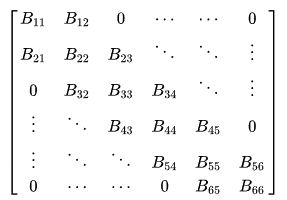
\includegraphics[width = 7cm]{images/lec6-1.png}
    \caption{A band matrix (tridiagonal) with $\operatorname{bw}=1$}
\end{figure}

\subsection{Symmetric (Hermitian) Positive Definite}
\begin{definition}
    $A$ is real and symmetric positive definite if and only if $A=A^\top$ and $x^\top Ax > 0$ for all $x \neq 0$.\\
    $A$ is complex and Hermitian positive definite if and only if $A=A^H$ and $x^H Ax > 0$ for all $x \neq 0$.
\end{definition}

\begin{lemma}[Just for real case]
    \begin{enumerate}
        \item[]
        \item  $X$ nonsingular implies that $A$ is symmetric positive definite if and only if $X^\top AX$ is symmetric positive definite.\begin{proof}
            $A$ is symmetric positive definite and $x \neq 0$ implies that $Xx \neq 0$. Then $0\neq \left(Xx\right)^{\top} A\left(X{x}\right)$, 
            which means $X^\top AX$ is symmetric positive definite.
        \end{proof}
        \item $A$ is symmetric positive definite and $H = A(j:k,j:k)$ implies that $H$ is symmetric positive definite ($H$ called a "principal submatrix").\begin{proof}
            $A$ is symmetric positive definite and $y \neq 0$ implies that \begin{align*}
                0 \neq x = \left[\begin{array}{l}
                    0 \\
                    y \\
                    0
                    \end{array}\right],
            \end{align*}
            where $y$ in rows $j$ to $k$. Then, \begin{align*}
                x^\top Ax = y^\top Hy \neq 0
            \end{align*}
        \end{proof}
        \item $A$ is symmetric positive definite if and only if $A=A^\top$ and all $\lambda_i > 0$. \begin{proof}
            $A$ is symmetric implies that $AQ = Q\Lambda$ where $Q^{-1} = Q^\top$ and $\Lambda = \operatorname{diag}(\lambda_1, \cdots, \lambda_n)$. $A=Q\Lambda Q^\top$
            so $A$ is symmetric positive definite if and only if $\Lambda$ is symmetric positive definite.
        \end{proof}
        \item $A$ is symmetric positive definite implies that $A_{ii}>0$ and \begin{align*}
            \max _{i, j}|A_{ij}|=\max_{i} |A_{ii}|
        \end{align*}
        i.e. the largest entry is on diagonal.
        \begin{proof}
            Let
            \begin{align*}
                e_{i}=\left[\begin{array}{l}
                    0 \\
                    \vdots \\
                    1 \\
                    \vdots \\
                    0
                    \end{array}\right],
            \end{align*}then $e_{i}^{\top} A e_{i}=A_{ii}$. Suppose $A_{ij}$, $i \neq j$ were largest. Let $x$ be a vector of zeros except for $x_i=1$ and $x_j=-\operatorname{sign}(A_{ij})$.
            Then \begin{align*}
                x^\top Ax = A_{ii} + A_{jj} - 2 |A_{ij}| \leq 0,
            \end{align*}
            a contradiction.
        \end{proof}
        \item (Basis of Cholesky) $A$ is symmetric positive definite if and only if $A=LL^\top$ where $L$ is a lower triangular matrix with positive diagonal entries. \begin{proof}
            Prove by induction, showing Schur complement is symmetric positive definite. \begin{align*}
                A = \left[\begin{array}{ll}
                    A_{11} & A_{12} \\
                    A_{21} & A_{22}
                    \end{array}\right] = \left[\begin{array}{ll}
                    \sqrt{A_{11}} & 0 \\
                    A_{21} / \sqrt{A_{11}} & I
                    \end{array}\right] \cdot \left[\begin{array}{cc}
                        \sqrt{A_{11}} & A_{12} / \sqrt{A_{11}} \\
                        0 & S
                        \end{array}\right]
            \end{align*}
            where $A_{11}$ is a $1 \times 1$ matrix and \begin{align*}
                S&=A_{22}-A_{21} A_{12} / A_{11} \\
                &= \left[\begin{array}{ll}
                    \sqrt{A_{11}} & 0 \\
                    A_{21} / \sqrt{A_{11}} & I
                    \end{array}\right] \left[\begin{array}{ll}
                        1 & 0 \\
                        0 & S
                        \end{array}\right] \left[\begin{array}{ll}
                            \sqrt{A_{11}} & A_{21} / \sqrt{A_{11}} \\
                            0 & I
                            \end{array}\right] \\
                &= X \left[\begin{array}{ll}
                    1 & 0 \\
                    0 & S
                    \end{array}\right] X^\top
            \end{align*}
            So $\left[\begin{array}{ll}
                1 & 0 \\
                0 & S
                \end{array}\right]$ is symmetric positive definite implies that $S$ is symmetric positive definite.\\
            By induction, $S=L_S L_{S}^{\top}$. \begin{align*}
                A &= \left[\begin{array}{ll}
                    \sqrt{A_{11}} & 0 \\
                    A_{21} / \sqrt{A_{11}} & I
                    \end{array}\right] \left[\begin{array}{ll}
                        1 & 0 \\
                        0 & L_S L_{S}^{\top}
                        \end{array}\right] \left[\begin{array}{ll}
                            \sqrt{A_{11}} & A_{21} / \sqrt{A_{11}} \\
                            0 & I
                            \end{array}\right] \\
                &= \left[\begin{array}{ll}
                    \sqrt{A_{11}} & 0 \\
                    A_{21} / \sqrt{A_{11}} & L_S 
                    \end{array}\right] \left[\begin{array}{ll}
                            \sqrt{A_{11}} & A_{21} / \sqrt{A_{11}} \\
                            0 & L_{S}^{\top}
                            \end{array}\right] = LL^{\top}
            \end{align*}
            as desired.
        \end{proof}
    \end{enumerate}
\end{lemma}

\begin{definition}
    Suppose $A$ is symmetric positive definite, then $A = LL^{\top}$ with $L$ lower triangular with positive diagonal is called the Cholesky factorization.
\end{definition}

\begin{lemma}
    If $A$ is symmetric positive definite and $A=LU$ with $L$ unit lower triangular, let $D$ be diagonal with $D_{ii} = \sqrt{U_{ii}} > 0$.
    Then $A = (L D)\left(D^{-1} U\right) = L_S L_{S}^{\top}$ is the Cholesky factorization.
\end{lemma}

This lemma suggests that any algorithm for LU can be modified to do Cholesky, and in fact use half the work and space since $L$ and $U$ are simply related. 
\begin{algorithmfrm}[The simplest one]
    \begin{algorithmic}[1]
        \For{\texttt{$j=1:n$}}
                \State $L_{jj} = \left(A_{jj}-\sum_{i=1}^{u-1} L_{ji}^{2}\right)^{1 / 2}$
                \State $L_{j+1:n,j} = \left(A_{j+1:n,j}- L_{j+1:n,j-1} \cdot L_{j,1:j-1}^\top \right) / L_{jj}$
                \EndFor
    \end{algorithmic}
\end{algorithmfrm}

Error analysis: Same approach as to LU yields analogous bound:\begin{align*}
    (A+E)(x+\delta x)=b
\end{align*}
where $|E| \leq 3 n \varepsilon |L| |L^{\top}|$. But since we do not pivot, we need to use a different approach to bound $|L| |L^{\top}|$:\begin{align*}
    \left( |L| |L^{\top}| \right)_{ij} &= \sum_{k}\left|L_{i k}\right| \left|L_{j k}\right| \\
    &\leq \norm{L_{i,:}}\norm{L_{j,:}} \\
    &= \sqrt{A_{ii}}\sqrt{A_{jj}} \\
    &\leq \text{the max entry in }A
\end{align*}

\subsection{Symmetric Indefinite}
It is also possible to save half the space and flops by just preserving symmetry, without assuming positive definiteness.
The traditional approach is called Bunch-Kaufman factorization:
\begin{align*}
    A = PLDL^\top P^\top
\end{align*} where $P$ is a permutation, $L$ is unit lower triangular, and $D$ has 1-by-1 and 2-by-2 diagonal blocks.
More complicated pivoting (with 2x2 blocks) is needed to preserve symmetry: consider $A=\left[\begin{array}{ll}
    0 & 1 \\
    1 & 0
    \end{array}\right]$. Instead of just searching a column for a pivot, once needs to search along a row too.
It is more complicated to apply ideas from LU and Cholesky to this factorization (blocking, recursion, communication lower bounds):
see \textit{LAPACK} routine \textit{ssytrf}.

A more numerically stable version is called rook-pivoting, which may search more than one row and column of $A$, 
but has better numerical stability guarantees, see \textit{LAPACK} routine \textit{ssytrf}.

And there is another approach (called Aasen factorization):
$$A = PLTL^\top P^\top$$ where now $T$ is a symmetric tridiagonal matrix, and so costs just $O(n)$ to solve $Tx=b$. 
See \href{https://ieeexplore.ieee.org/stamp/stamp.jsp?arnumber=6569872}{"Implementing a Blocked Aasen's Algorithm with A Dynamic Scheduler on Multicore Architectures"}. 
Aasen is more amenable to optimizations to minimize communication.

\subsection{Band Matrices}

These are the simplest sparse matrices, and have solvers in \textit{LAPACK}. 
\begin{itemize}
    \item Case without pivoting (e.g. Cholesky):
    $A=LU$, $L$, $U$ bounded. $\operatorname{ubw}(U)=\operatorname{ubw}(A)$, $\operatorname{lbw}(U)=\operatorname{lbw}(A)$.
    The cost is $2n \cdot \operatorname{ubw} \cdot \operatorname{lbw} + n \cdot \operatorname{lbw}= O(n)$ for narrow bandwidths.
    \item Case with pivoting: $A=PLU$,
    $\operatorname{ubw}(U)=\operatorname{ubw}(A) + \operatorname{lbw}(A)$, 
    $"\operatorname{lbw}(L)" = \operatorname{lbw}(A)$ (does not look banded, but uses same amount of storage)
\end{itemize}

\begin{figure}
    \centering
    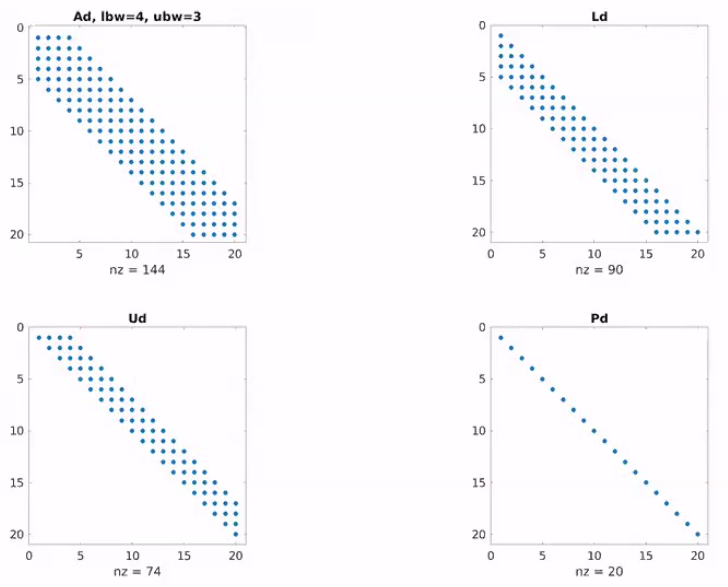
\includegraphics[width = 10cm]{images/lec6-2.png}
    \caption{Case without pivoting}
\end{figure}

\begin{figure}
    \centering
    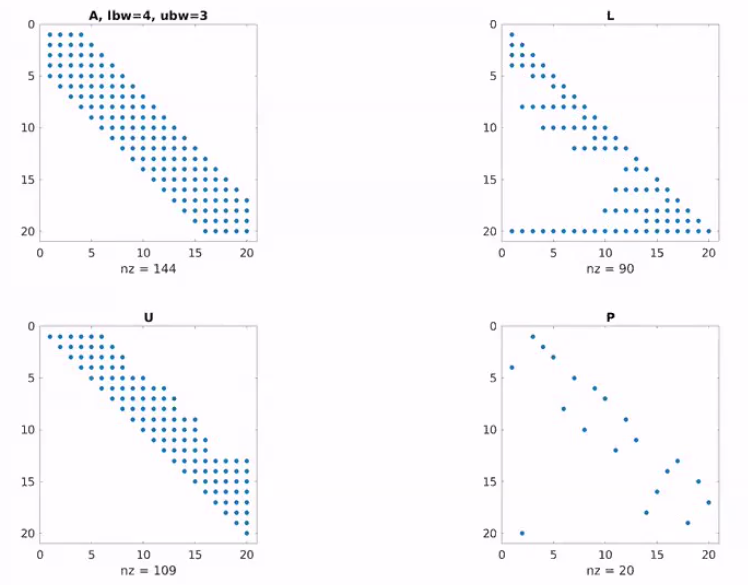
\includegraphics[width = 10cm]{images/lec6-3.png}
    \caption{Case with pivoting}
\end{figure}

Band matrices often arise from discretizing differential equations, or other physical simulations, where each unknown only depends on its neighbors, 
so $A_{ij}$ is nonzero only when $i$ and $j$ are close, i.e. $A_{ij}$ near diagonal.

\begin{theorem}[Gershgorin's Theorem]\label{thm:Gershgorin}
    All eigenvalues lambda of $A$ lie in $n$ circles in the complex plane, where circle $i$ has center $A_{ii}$ and radius $\sum_{j=1, j \neq i}^{n} |A_{ji}|$.
    \begin{proof}
        If $A x=\lambda x$, suppose $|x_i|$ is the largest entry in absolute value of $x$. Thus, \begin{align*}
            A_{ii}-\lambda &= \sum_{j=1, j \neq i}^{n} \frac{A_{ji} x_j}{x_i}
        \end{align*}
        and so \begin{align*}
            |A_{ii}-\lambda| &\leq \sum_{j=1, j \neq i}^{n} |A_{ji}| |{ x_j}/{x_i}| \\
            &\leq \sum_{j=1, j \neq i}^{n} |A_{ji}|
        \end{align*}
    \end{proof}
\end{theorem}

\begin{example}[Sturm-Liouville problem]
    $ -y"(x) + q(x) y(x) = r(x)$ on $x \in[0,1]$, $y(0)=\alpha$, $y(1)=\beta$, $q(x) \geq \bar{q}>0$, discretize at $x(i)=ih$, $h = \frac{1}{N+1}$. 
    Unknowns $y(i)=y(x(i))$ for $i=1, \cdots, N$. Approximate \begin{align*}
        y"(i)= \frac{(y(i+1)-2 y(i)+y(i-1))}{h^2}
    \end{align*}
    So, letting $q(i)=q(x(i))$ and $r(i)=r(x(i))$, we get linear system \begin{align*}
        \frac{-(y(i+1)-2 y(i)+y(i-1))}{h^2}+g(i) y(i)=r(i)
    \end{align*} or $Ay=v$ where \begin{align*}
        v &= r+\left[\frac{\alpha}{h^{2}}, 0, \ldots 0, \frac{\beta}{h^{2}}\right] \\
        A &= \operatorname{diag}(\frac{2}{h^2} + q(i)) + \operatorname{diag}(\frac{-1}{h^2} ,1) + \operatorname{diag}(\frac{-1}{h^2} ,-1)
    \end{align*}
    We can prove $A$ is symmetric positive definite, so we can use Cholesky, by using the theorem \ref{thm:Gershgorin} (Gershgorin's Theorem) to $A=A^\top$,
    all eigenvalues in circles centered at $2/h^2 + q(i) >= 2/h^2 + \bar{q}$, with radius $2/h^2$, so must be real and positive.
\end{example}

\begin{example}
    Now consider Poisson's equation in 2 dimensions:\begin{align*}
        \frac{\partial^{2} u(x, y)}{\partial x^{2}}+\frac{\partial^{2} u(x, y)}{\partial y^{2}}+g(x, y) u(x, y)=r(x, y)
    \end{align*}
    in a square $0 \leq x,y \leq 1$ with boundary conditions: $u(x,y)$ given on the boundary of square.\\
    Typical example: Given temperature on boundary of a square of uniform material, what is the temperature everywhere in the middle ($q=r=0$)? \\
    We discretize the square with an $n\times n$ mesh: $h=1/(n+1)$, $x(i)=ih$, $y(i)=ih$, $u(i,j)=u(x(i), y(i))$, same for $4q(i,j)$ and $r(i,j)$.
    Again approximate \begin{align*}
        \frac{\partial^{2} {u}(x y)}{\partial x^{2}} &\cong[u(x-h, y)-2 u(x, y)+u(x+h, y)] / h^{2} \\
        \frac{\partial^{2} {u}(x y)}{\partial y^{2}} &\cong[u(x, y-h)-2 u(x, y)+u(x, y+h)] / h^{2}
    \end{align*}
    Add these, evaluate at $(x(i), y(i))$, so \begin{align*}
        \frac{\partial^{2} u(x, y)}{\partial x^{2}}+\frac{\partial^{2} u(x, y)}{\partial y^{2}} \approx \left[ u(i-1, j) + u(i+1, j) + u(i, j-1) + u(i, j+1) -4u(i,j) \right] / h^2
    \end{align*}
    Using "natural order" (rowwise or columnwise ordering of mesh points $(i,j)$), we get an spd band matrix of dimension $n^2$ and bandwidth $n$.
    $A$ is banded but at with most 5 nonzeros per row, so should really think of it as sparse.
\end{example}

\subsection{General Sparse Matrices}
Here is a small \textit{MATLAB} example to show important of ordering on "arrowhead matrix":
\begin{minted}{matlab}
    A = eye(8);A(1,2:8)=.1;A(2:8,1)=.1;
    [L,U]=lu(A);A,L,U,
    figure(1), clf, spy(A,'k'), pause
    spy(L,'b'), hold on, spy(U,'r'), spy(A,'k')
\end{minted}
Result is dense! So performing LU and storing $L$ and $U$ would cost as many flops and words as a dense matrix, $O(n^3)$ and $O(n^2)$. 

\begin{figure}[h]
    \centering
    \begin{subfigure}{.5\textwidth}
      \centering
      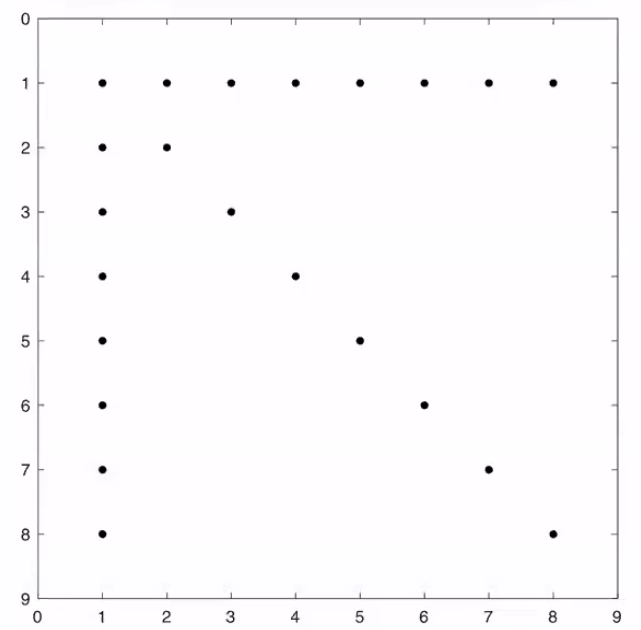
\includegraphics[width=.4\linewidth]{images/lec6-4.png}
      \caption{The original "arrowhead matrix"}
    \end{subfigure}%
    \begin{subfigure}{.5\textwidth}
      \centering
      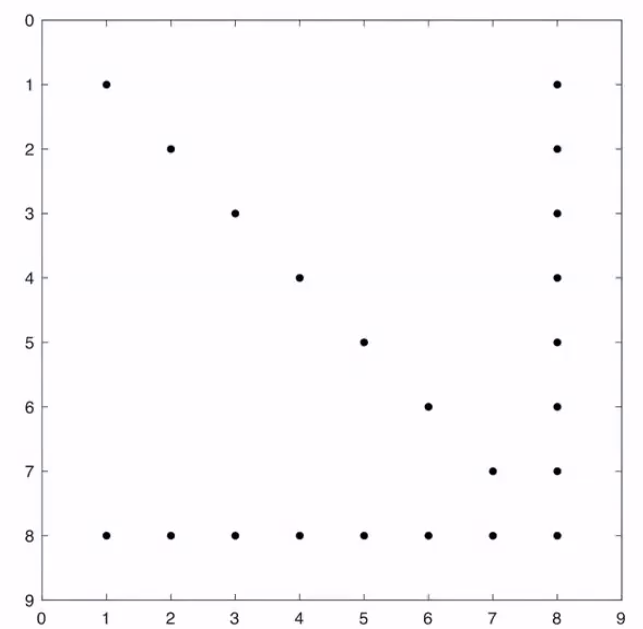
\includegraphics[width=.4\linewidth]{images/lec6-5.png}
      \caption{The reversed "arrowhead matrix"}
    \end{subfigure}
    \caption{\textit{MATLAB} results for "arrowhead matrix"}
\end{figure}

Now let's try LU on $PAP^\top$, where $P$ is a permutation that reverses the order of rows and columns.
\begin{minted}{matlab}
    Arev=A(8:-1:1,8:-1:1);
    [Lrev,Urev]=lu(Arev); Arev, Lrev, Urev
    figure(2), clf, spy(Arev,'k'), pause
    spy(Lrev,'b'), hold on, spy(Urev,'r'), spy(Arev,'k')
\end{minted}
Result is very sparse! And if you rewrite LU to take advantage of this, to neither store nor compute entries that are certain to be zero, 
the cost in flops and words would drop to $O(n)$, much smaller than before. \textit{MATLAB} has many built-in sparse matrix operations (LU, Cholesky, etc), 
that take advantage of sparsity like this; do "help sparse" to learn more.

Let's see what happens to the 2D Poisson equation:
\begin{minted}{matlab}
    A = TwoDL(6); R = chol(-A); L = R'; 
    \cdots R = upper triangular Cholesky factor
    figure(1), clf, spy(L,'b'),hold on, spy(A,'k')
\end{minted}

\begin{figure}[h]
    \centering
    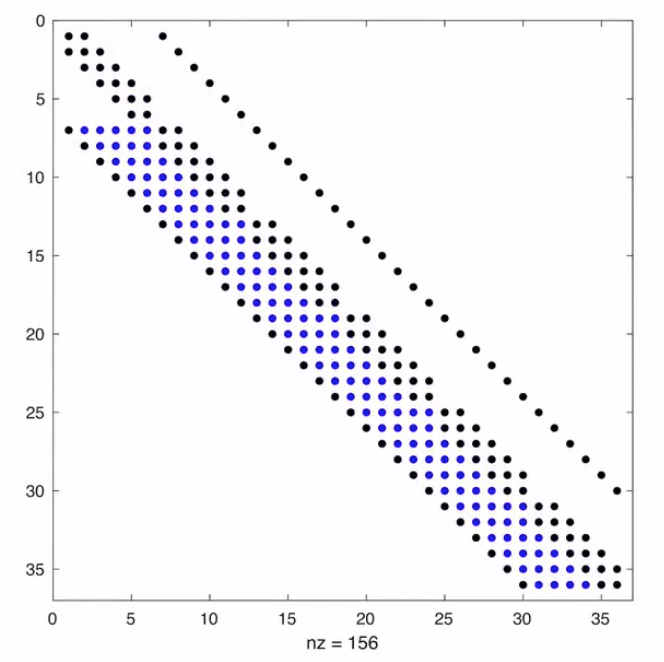
\includegraphics[width = 7cm]{images/lec6-6.png}
    \caption{\textit{MATLAB} result for 2D Poisson equation}
\end{figure}

So the band fills in entirely, costing \begin{align*}
    O(N \operatorname{bw}^2) = N\sqrt(N)^2 = N^2 = n^4
\end{align*}
for an $n\times n$ mesh with $N = n^2$ unknowns. We'll see that we can do much better, $O(n^3)$ instead, for a clever choice of permutation $P$ in $PAP^\top$.

\begin{definition}
    A weighted, undirected graph $G$ is a collection of 3 sets: \begin{itemize}
        \item $V$: Vertices (as known as nodes)
        \item $E$: Edges connected pairs of vertices $(u,v)$ (note: $(u,u)$ is allowed; undirected means $(u,v)$ is the same as $(v,u)$
        \item $W$: Weight (number) associated with each edge
    \end{itemize}
\end{definition}

There is an obvious one-to-one relationship between a weighted undirected graph $G$ and a symmetric matrix, and we will use the notations interchangeably: \begin{itemize}
    \item $V$: One row and column per vertex
    \item $E$: Locations of nonzeros (note: $(u,u)$ on diagonal)
    \item $W$: Values of nonzeros
\end{itemize}

\subsection{Challenges to Factoring Sparse Matrices}
Store and operate on only nonzeros in an efficient way. The simplest imaginable data structure is Coordinate Format (COO):
list of nonzero entries and their locations $(a(i, j), i, j)$.
\begin{example}
    For matrix \begin{align*}
        A=\left[\begin{array}{lllll}
            2 & 0 & 2 & 0 & 5 \\
            0 & 1 & 4 & 0 & 3 \\
            0 & 0 & 8 & 0 & 0
            \end{array}\right],
    \end{align*}its $\operatorname{COO} = ((2,1,1),(7,1,3),(5,1,5),(1,2,2),(4,2,3),(3,2,5),(8,3,3))$.
\end{example}

A better way is  Compressed Sparse Row (CSR):\begin{itemize}
    \item $\mathrm{val}$: The array of nonzero entries in each row, from row $1$ to row $n$, from left to right
    \item $\mathrm{col\_index}$: Columns index of each nonzero ($\mathrm{val}(i)$ is in $\mathrm{col}(a)$ of sparse matrix)
    \item $\mathrm{rowbegin}$: The pointer to start of each row: entries of row $i$ lies in entries $\mathrm{rowbegin}(i)$ through $\mathrm{rowbegin}(i+1)-1$ of $\mathrm{val}()$ and $\mathrm{col}()$
\end{itemize}

\begin{example}
    With the same matrix from the above example, its $\mathrm{CSR}$ is \begin{align*}
        &\mathrm{val} = (2, 7, 5, 1, 4, 3, 8) \\
        &\mathrm{col\_index} = (1, 3, 5, 2, 3, 5, 3) \\
        &\mathrm{rowbegin} = (1, 4, 7, 8) 
    \end{align*}
\end{example}

We want to minimize time, memory, get the right answer (stability). Order effects fill-in, which effects time and memory (less is better!).
So we want to pick order to minimize fill-in. Order effects backward stability for LU (and symmetric indefinite $LDL^\top$), 
but not Cholesky (recall that the stability proof for Cholesky did not depend on order).
Cholesky is easiest case: can pick order just to minimize fill in.

What is the best order for Cholesky, i.e. choose permutation $P$, do Cholesky on $P$, do Cholesky on $PAP^\top$ to minimize flops.

\begin{theorem}
    Picking the optimal order (out of all n! possibilities) is NP-hard, i.e. any algorithm will have cost exponential in $n$, overwhelming everything else.
\end{theorem}

\begin{definition}
    A path in a graph from vertex $v_1$ to $v_k$ is a set of edges $(v_1,v_2),(v_2,v_3), \cdots , (v_{k-1},v_k)$ connected end-to-end.
\end{definition}

\begin{definition}
    The degree of a vertex in the graph is the number of edges for which it is an endpoint.
\end{definition}

\begin{definition}
    The distance between any two vertices is the length of the shortest path (fewest edges) connecting them.
\end{definition}

So we need to use heuristics:\begin{itemize}
    \item Reverse Cuthill-McKee (RCM / Breadth-First Search): \begin{enumerate}
        \item Pick any vertex, call it the root.
        \item Compute distance of all other vertices from root, and label them by distance, (so $\mathrm{distance}=0$ is the root, 
        $\mathrm{distance}=1$ are the vertices with an edge to the root, etc), $\mathrm{Cost}=0$(\#nonzeros in matrix), 
        using Breadth-First-Search, cheap!
        \item Order vertices in reverse order by distance (farthest first)
    \end{enumerate}
    \begin{fact}
        Vertices at distance $k$ can only be directly connected to vertices at distance $k-1$ or $k+1$ (otherwise distance would be wrong!)
        Explains why RCM ordering tends to make matrix entries close to diagonal: matrix becomes block tridiagonal,
         with vertices at distance $k$ making up diagonal block k. So it is like a band matrix, and limits fill-in to the band. 
    \end{fact}
    Called \textit{symrcm} in \textit{MATLAB}.
    \item Minimum Degree (MD): At each step pick pivot to have minimum degree (note: as factorization proceeds, need to update matrix and its graph, so degree can change; use latest degree)
    \begin{fact}
        If vertex corresponding to row/column $i$ is used as a pivot, and has degree $d$, then we need to do $d^2$ multiplications and adds, 
        and so can fill in at most $d^2$ entries (if they were originally zero, and ignoring symmetry).
    \end{fact}
    \item Nested Dissection: "Bisect" vertices of graph into 3 sets $V = V_1 \cup V_2 \cup V_s$ (s stands for "separator") such that:\begin{enumerate}
        \item About the same number of vertices in $V_1$ and $V_2$
        \item $V_s$ much smaller than $V_1$ and $V_2$
        \item There are no edges directly connecting vertices in $V_1$ and $V_2$
    \end{enumerate}
    Now reorder vertices with $V_1$ first, then $V_2$, then $V_s$:\begin{align*}
        A = \left[\begin{array}{lll}
            A_{11} & 0 & A_{1s} \\
            0 & A_{21} & A_{23} \\
            A_{13}^\top & A_{23}^\top & A_{33}
            \end{array}\right],
    \end{align*}
    so after Cholesky, \begin{align*}
        L = \left[\begin{array}{lll}
            L_{1} & 0 & 0 \\
            0 & L_2 & 0 \\
            L_{1s} & L_{2s} & L_{s}
            \end{array}\right],
    \end{align*}
    in particular, $A_1 = L_1 L_1^\top$ and $A_2 = L_2 L_2^\top$ are independent Cholesky factorizations.
\end{itemize}

\begin{theorem}[George, Hoffman/Martin/Rose, Gilbert/Tarjan, 1970s \& 1980s]
    Any ordering for Cholesky on a 2D $n \times n$ mesh (so the matrix is $n^2 \times n^2$) has to do at least $\Omega(n^3)$ flops,
    and this is attained by nested dissection ordering. (If it were dense, it would cost $O(n^6)$, a lot more).
    This extends to "planar graphs", i.e. graph you can draw on paper without crossing any edges.    
\end{theorem}

\begin{theorem}[Ballard, Demmel, Holtz, Schwarz, 2009]
    Lower bound on $\#\mathrm{words}$ moved for sparse LU and Cholesky is $\Omega(\#\mathrm{flops} / \sqrt{M})$, where $\#\mathrm{flops}$ is number actually performed. 
    So the lower bound on $\#\mathrm{words\_moved}$ for Cholesky on $n \times n$ mesh is $\Omega(n^3/\sqrt{M})$.
\end{theorem}

\begin{theorem}[David, D., Grigori, Peyronnet 2010]
    Possible to achieve lower bound for $n \times n$ of $\Omega(n^3/\sqrt{M})$ words moved by Cholesky with nested dissection ordering, if properly implemented.
\end{theorem}

Contrast: band solver would cost $O(dimension* \operatorname{bw}^2) =n^{2+2}=n^4$ flops.

It's a good idea for 3D meshes too: $n \times n \times n$ mesh (so matrix is $n^3$ by $n^3$) costs $n^6$ to factor using Cholesky with nested dissection ordering 
(versus $n^9$ if it were dense, or $n^{3+2+2}=n^7$ if banded).

\subsection{Summarize Sparse Cholesky}
To summarize, the overall sparse Cholesky algorithm is as follows:\begin{itemize}
    \item Choose ordering (RCM, MD, ND)
    \item Build data structure to hold $A$ and (to be computed) entries of $L$
    \item Perform factorization
\end{itemize}

\begin{theorem}
    For any $A$ there is a permutation $P$ and diagonal matrices $D_1$ and $D_2$ such that $B = DD_1 A P D_2$ has $B_{ii} = 1$ and all other $|B_{ij}| \leq 1$.
\end{theorem}

What about nonsymmetric matrices, how do we pivot for sparsity and stability?\begin{itemize}
    \item Threshold pivoting: among pivot choices in column within a factor of 2 or 3 of the largest, pick the one with the least fill-in 
    (so may need to change data structure on the fly).
    \item Static Pivoting (used in \textit{SuperLU\_DIST}): 
    \begin{enumerate}
        \item Permute and scale matrix to try to make diagonal as large as possible
        \item Reorder using similar ideas as for Cholesky: this leaves all the diagonal entries on the diagonal. Then build the data structures for $L$ and $U$, 
        before doing LU, rather than figuring them out on the fly, which would be slower.
        \item During factorization, if a prospective pivot is too small, just make it big (This happens rarely in practice). 
        As a result we get the LU factorization of $A + a$ low rank change (the rank = the number of modified pivots), which we can fix with the Sherman-Morrison-Woodbury formula or an iterative method like GMRES.
    \end{enumerate}
\end{itemize}

This brief discussion suggests that there is a large body of software that has been developed for solving sparse $Ax=b$, 
and which one is faster may depend on your matrix (and computer). There is a survey of available sparse matrix software:
\href{http://crd.lbl.gov/~xiaoye/SuperLU/SparseDirectSurvey.pdf}{"Updated Survey of sparse direct linear equation solvers"}.

Finally, we give a brief tour of structured matrices, which may be dense but depend only on $O(n)$ parameters. The number of structures that can arise, 
and be used to get faster algorithms, is large, e.g. depending on the underlying physics of the problem being modeled.
We will do one set of common examples that share a structure:\begin{itemize}
    \item Vandermonde: $V_{ij} = x_i^{j-1}$ - arises in polynomial interpolation
    \item Cauchy: $C_{ij} = 1/(x_i+y_j)$ - arises in rational interpolation
    \item Toeplitz: $T_{ij} = x_{i-j}$, constant along diagonals, arises in convolution
    \item Hankel: $H_{ij} = x_{i+j}$, constant along "anti-diagonals", similar to Toeplitz
\end{itemize}

E.g.: Solving $Vz = b$ means \begin{align*}
    \sum_{j=1}^n x_i^{j-1} z_j = b_i
\end{align*} i.e. finding polynomial coefficients $z_j$ so to match values $b_i$ at points $x_i$, i.e. polynomial interpolation; 
we know how to do this in $O(n^2)$ time using, eg using "Newton interpolation." Another trick works for $V^\top z = b$.

E.g.: Multiplying by a Toeplitz matrix is same as convolution, which we know how to do fast by FFT.

E.g.: Solving with a Cauchy, also interpretable as interpolation.

Common structure of $X$: $AX + XB$ = low rank for some simple, nonsingular $A$ and $B$.

\begin{definition}
    The rank is called the "displacement rank".
\end{definition}

\begin{example}
    Let $D = \operatorname{diag}(x_i)$, then $DV$ is "$V$ shifted left",
    \begin{align*}
        V P = V \left[\begin{array}{llll}
            0 & 0 & & 1 \\
            1 & 0 & & 0 \\
            0 & 1 & \ddots & 1 \\
            \vdots & 0 & & 0 \\
            0 & \vdots & & 0
            \end{array}\right]
    \end{align*} is "$V$ shifted left",
    difference $DV - VP$ is zero except the last column, then the rank is 1.  
\end{example}

\begin{example}
    $T$ Toeplitz implies that $PT - TP = T$ shifted down then $T$ shifted left,
    nonzero are only in first row, last col, then the rank is 2.
\end{example}

\begin{example}
    $C$ Cauchy implies that $\operatorname{diag}(x_i) C + C\operatorname{diag}(y_i)$ are all ones, then the rank is 1.     
\end{example}

\begin{theorem}[Kailath et al.]
    There are $O(n^2)$ solvers if displacement rank low (stability can be a problem).
\end{theorem}

\begin{theorem}[George \& Liu, 1981]
    $L_{ij}$ is nonzero (assuming no exact cancellation) if there is a path from $i$ to $j$ in the graph $G$ of $A$ passing through vertices $k$ satisfying $k < i$ and $k < j$.
\end{theorem}

\begin{theorem}[Gilbert \& Peierls]
    Cost of determining structure of $L$ no more than actually doing the factorization.
\end{theorem}

\newpage
\section{Lecture 7: Least Squares}
\subsection{Introduction to Least Squares}
Standard notation:
 $$ \underset{x}{\arg\min} \| Ax-b \|_2, \ A \ m \times n, \ m > n $$
 $m > n$ means overdetermined, don't expect $Ax=b$ exactly. 
 Other variants of Least Squares::
 \begin{itemize}
     \item Constrained: $ \underset{x: \ Bx=y}{\arg\min} \| Ax-b \|_2$ where $\#\mathrm{rows}(B) \leq \#\mathrm{cols}(A) \leq \#\mathrm{rows}(A) + \#\mathrm{rows}(B)$. So answer unique if $A,B$ full rank
     \item Weighted Least Squares:: $ \underset{x}{\arg\min} \| y \|_2$ such that $b=A x+B y$. It is weighted because if $B=I$, it would be usual LS. If $B$ square, nonsingular, $ \underset{x: \ Bx=y}{\arg\min} \| B^{-1}(Ax-b) \|_2 $
     \item Underdetermined: $\#\mathrm{rows}(A) < \#\mathrm{cols}(A)$ or if $A$ is not full column rank, then there is a whole space of solutions (add any $z$ such that $Az=0$ to $x$). To make solution unique, $\underset{x}{\arg\min} \| x \|_2$
     such that $Ax=b$
     \item Ridge Regression: $\underset{x}{\arg\min} \| Ax-b \|_2^2 + \lambda \| x \|_2^2$, guarantees unique solution if $\lambda >0$
     \item Total Least Squares: $\underset{x}{\arg\min}(A+E)x = b + r$, $\norm{[E, r]}_2$
 \end{itemize}

\subsection{Algorithm for Overdetermined Cases}
\begin{itemize}
    \item Solve Normal Equations (NE): $A^{\top} A{x}=A^{\top} b$, $A^{\top}A$ s.p.d $\implies$ solve with Cholesky, the fastest in dense case, not stable if $A$ ill-conditioned
    \item Use QR Decomposition: $A=QR$, $Q$ is $m \times n$ and has orthonormal columns, $R$ is upper triangular.
    \begin{itemize}
        \item Gram-Schmidt: Unstable if $A$ ill-conditioned
        \item Householder: Stable ($x=A\backslash b$ in \textit{MATLAB})
        \item Blocked Householder: Reduce data movement
        \item Cholesky QR: Getting QR via Normal Equations, fast but can be unstable.
    \end{itemize} 
    \item SVD: most "complete answer", gives condition number, error bounds, works in ill-conditioned, rank deficient cases too.
    \item Conversion to a linear system, where matrix contains $A$, $A^\top$, not $A^\top A$, allows us to exploit sparsity, iterative refinement (also possible to exploit sparsity in QR).
\end{itemize}

\subsubsection{Normal Equations}
\begin{theorem}[Normal Equations]
    If $A$ full column rank, solution of $A^\top Ax = A^\top b$ minimizes $\norm{Ax-b}_2$.
    \begin{proof}
        Assume $x$ satisfies NE.
        \begin{align*}
            \sqnorm{A(x + e)-b} &= (A(x + e)-b)^\top (A(x + e)-b) \\
            &= (Ax-b+Ae)^\top(Ax-b+Ae) \\
            &= (Ax-b)^\top(Ax-b) + 2e^\top A^\top(Ax-b) + (Ae)^\top(Ae) \\
            &= \sqnorm{Ax-b} + 0 + \sqnorm{Ae}
        \end{align*}
        which is minimized at $e=0$.
    \end{proof}
\end{theorem}

\subsubsection{QR Decomposition}
$A=QR$, where $A$ is $m \times n$, $Q$ is $m \times n$ and has orthonormal columns, $R$ is $n \times n$ and upper triangular. To minimize $\norm{Ax-b}_2$,
$x=R^{-1}Q^\top b$.
\begin{proof}[proof 1]
    $A=QR=\left[ Q, \hat{Q} \right]\left[ R, 0 \right]^\top$, where $\left[ Q, \hat{Q} \right]$ is square and orthogonal. Then \begin{align*}
        \sqnorm{Ax-b} &= \sqnorm{\left[ Q, \hat{Q} \right]^\top (Ax-b)} \\
        &= \sqnorm{\left[\begin{array}{l}
            Q^{\top} Q R{x}-Q^\top b \\
            \hat{Q}^{\top} Q R {x}-\hat{Q}^{\top} b
            \end{array}\right]} \\
        &= \sqnorm{\left[\begin{array}{l}
            R{x}-Q^\top b \\
            -\hat{Q}^{\top} b
            \end{array}\right]} = \sqnorm{R{x}-Q^\top b} + \sqnorm{\hat{Q}^{\top} b}
    \end{align*}
    which is minimized when $x = R^{-1} Q^{\top} b$.
\end{proof}

\begin{proof}[proof 2]
    Plug into normal equations: \begin{align*}
        x &= \left(A^{\top} A\right)^{-1} A^{\top} b \\
        &= \left(R^{\top} Q^{\top} Q R\right)^{-1} R^{\top} Q^{\top} b \\
        &= \left(R^{\top} R\right)^{-1} R^{\top} Q^{\top} b \\
        &= R^{-1} R^{\top} R^{\top} Q^{\top} b = R^{-1} Q^\top b
    \end{align*}
\end{proof}

Algorithms for computing $A=QR$:
\begin{itemize}
    \item Classical \textit{Gram-Schmidt}: Much much less stable than the modified one.
    \item Modified \textit{Gram-Schmidt}:
    \begin{savenotes}
        \begin{algorithmfrm}[Modified \textit{Gram-Schmidt}]
            \begin{algorithmic}[1]
                \State Equate columns $i$ of $A$ and $QR$ to get $A(:,i) = \sum^{i}_{j=1} Q(:,j)R(j,i)$
                \State $(Q(:,j))^\top A(:,i) = R(j,i)$
                \For{$j=1:n$}
                    \State $\mathrm{tmp}=A(:,i)$
                    \For{$j=1:i-1$}
                        \State $R(j,i) = Q(:,j)^\top A(:,i)$\Comment{CGS\footnote{Classical \textit{Gram-Schmidt}}, costs $2m$}
                        \State $R(j,i) = Q(:,j)^\top \mathrm{tmp}$\Comment{MGS\footnote{Modified \textit{Gram-Schmidt}}, costs $2m$, getting same result}
                        \State $\mathrm{tmp} = \mathrm{tmp} - R(j,i)Q(:,j)$\Comment{Costs $2m$}
                    \EndFor
                    \State $R(i,i) = \norm{\mathrm{tmp}}_2$\Comment{Costs $2m$}
                    \State $Q(:,i) = \mathrm{tmp} /R(i,i)$\Comment{Costs $m$}
                \EndFor
            \end{algorithmic}
        \end{algorithmfrm}
    \end{savenotes}
\end{itemize}

Two metrics of backward stability:\begin{itemize}
    \item[] If backward stable should get accurate QR decomposition of slight perturbed input matrix $A+E = QR$ where \begin{align*}
        \frac{\norm{E}}{\norm{A}} = O(\varepsilon)
    \end{align*}
    \item This means $\norm{QR-A}/\norm{A}$ should be $O(\varepsilon)$. 
    \item It also means $\norm{Q^\top Q-I}$ should be $O(\varepsilon)$, an extra condition.
\end{itemize}

\subsubsection{Singular Value Decomposition}
\begin{theorem}
    Suppose $A$ is an $ m \times m$ matrix. Then there exists orthogonal matrix $U=\left[u_1, \cdots, u_m\right]$, diagonal matrix $\Sigma=\operatorname{diag}\left(\sigma_1, \cdots, \sigma_m\right)$, $\sigma_1 \geq \sigma_2 \geq \cdots \geq \sigma_m \geq 0$,
    and an orthogonal matrix $V=\left[v_1, \cdots, v_m\right]$ such that $A=U\Sigma V^\top$.

    More generally, $A$ is an $ m \times n$ matrix, where $m>n$, $U$ is an $ m \times m$ matrix and is orthogonal as before, $V$ is a $ n \times n$, orthogonal matrix,
    $\Sigma$ is an $ m \times n$ matrix with same diagonal. When $m>n$, sometimes write as following (thin SVD): \begin{align*}
        A = \left[ u_1, \cdots, u_n \right] \operatorname{diag}\left(\sigma_1, \cdots, \sigma_n\right) V^\top = \hat{U}\hat{\Sigma}V^\top
    \end{align*}
\end{theorem}

\begin{definition}
    If $A=\hat{U}\hat{\Sigma}V^\top$, its Moore–Penrose pseudoinverse is \begin{align*}
        A^{+}=V \hat{\Sigma}^{-1} \hat{U}^{\top}
    \end{align*}
\end{definition}

\begin{fact}
    $A^{+}=\left(A^{\top} A\right)^{-1} A^{\top}$ because SVD and normal equations both solve least squares.
\end{fact}

\subsubsection{Perturbation Theory for Least Squares Problem}
If $x=\underset{x}{\arg \min} = \norm{Ax-b}_2$, and we change $A$ and $b$ a little, how much can $x$ change? 
Since square case is special case, expect $\kappa(A)$ to show up, but there is another source of sensitivity: \begin{align*}
    &A=\left[\begin{array}{l}
        1 \\
        0
        \end{array}\right], b=\left[\begin{array}{l}
        0 \\
        b_{2}
        \end{array}\right] \Rightarrow x= \left[ 1,0 \right] \left[\begin{array}{l}
        0 \\
        b_{2}
        \end{array}\right]=0 \\
    &A=\left[\begin{array}{l}
        1 \\
        0
        \end{array}\right], b=\left[\begin{array}{l}
        b_{1} \\
        b_{2}
        \end{array}\right] \Rightarrow x=\left[ 1,0 \right]\left[\begin{array}{l}
        b_{1} \\
        b_{2}
        \end{array}\right]=b
\end{align*}
If $b_2$ very large, $b_1$ could be small compared to $b_2$ but still large, so a big change in $x$. More generally, 
if $b$ is (nearly) orthogonal to $\operatorname{span}(A)$, then condition number very large.

Expand \begin{align*}
    e &= (x+e) - x  \\
    &= \left( (A+\delta A)^\top (A+\delta A) \right)^{-1} (A+\delta A)^\top (b+\delta b) - (A^\top A)^{-1}A^\top b
\end{align*}
using approximation $(I-X)^{-1}=I+X+O(\norm{X}^2)$ as before, only keeping linear terms (one factor of $\delta A$ and/or $\delta b$), call \begin{align*}
    \varepsilon = \max\left( \frac{\norm{\delta A}}{\norm{A}}, \frac{\norm{\delta b}}{\norm{b}} \right)
\end{align*} to get \begin{align*}
    \frac{\norm{e}}{\norm{x}} \leq \varepsilon \left( 2 \kappa (A) \frac{1}{\cos \theta} + \tan \theta \kappa^2(A) + O(\varepsilon^2) \right)
\end{align*}
where $\theta=\operatorname{angle}(b, Ax)$, or \begin{align*}
    \sin \theta = \frac{\norm{Ax-b}_2}{\|b\|_{2}}
\end{align*}
So condition number can be large if \begin{enumerate}
    \item $\kappa(A)$ large
    \item $\theta$ near $\pi/2$, i.e. $\frac{1}{\cos \theta} \sim \tan(\theta)$ large
    \item error like $\kappa^2(A)$ when theta not near zero
\end{enumerate}

Will turn out that using the right QR decomposition, or SVD, keeps $\varepsilon = O(\varepsilon)$, so backward stable. 
Normal equations are not backward stable; since we do $\operatorname{Chol}(A^\top A)$ the error bound is always proportional to $\kappa^2(A)$, even when $\theta$ small.

\subsection{Stable Algorithms for QR Decomposition}
Recall that MGS and CGS produced $Q$ that were far from orthogonal, and running them twice helped but sometime also failed to guarantee orthogonality.
\footnote{MGS still has its uses in some other algorithms, CGS does not.}

To guarantee stability of solving least squares problems (and later eigenproblems and computing the SVD) we need algorithms that guarantee that $Q$ is (very nearly) orthogonal, 
i.e. \begin{align*}
    \norm{Q^\top Q - I} = O(\varepsilon)
\end{align*}

The basic idea is to express $Q$ as product of simple orthogonal matrices $Q=Q_1 Q_2 \cdots Q_n$ where each $Q_i$ accomplishes part of the task
(multiplying it by $A$ makes some entries zero, until $A$ turns into $R$). Since a product of orthogonal matrices is orthogonal, there is no danger of losing orthogonality.
There are two kinds of simple orthogonal matrices: \textit{Householder transformations} and \textit{Givens rotations}.

\subsubsection{Householder Rotation}
A \textit{Householder transformation} (or reflection) is $H = I-2uu^\top$,
where $u$ is a unit vector. We confirm orthogonality as follows: \begin{align*}
    HH^\top = (I-2uu^\top )(I-2uu^\top ) = I - 4uu^\top + 4uu^\top uu^\top  = I
\end{align*}
It is called a reflection because $Hx$ is a reflection of $x$ in plane orthogonal to $u$.

\begin{figure}[h]
    \centering
    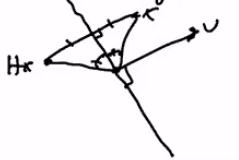
\includegraphics[width=5cm]{images/lec7-1.png}
    \caption{A reflection}
\end{figure}

Given $x$, we want to find $u$ so that $Hx$ has zeros in particular locations, in particular we want $u$ so that \begin{align*}
    Hx = \left[ c,0,0,\cdots, 0 \right]^\top = c \cdot e_1
\end{align*}
for some constant $c$. Since the $2$-norm of both sides is $\norm{x}_2$, then $|c| = \norm{x}_2$. We solve for $u$ as follows: Write \begin{align*}
    Hx = (I-2uu^\top)x = x - 2u(u^\top x) = c \cdot e_1,
\end{align*}
or 
\begin{align*}
    u = \frac{(x - c\cdot e_1)}{2u^\top x}.
\end{align*}
The denominator is just a constant that we can choose so $\norm{u}_2 = 1$, i.e. \begin{align*}
    y = x \pm \norm{x}_2 e_1 \text{ and }u = \frac{y}{\norm{y}_2}
\end{align*}
We write this as $u = \operatorname{House}(x)$. We choose the sign of $\pm$ to avoid cancellation (avoids some numerical problems) \begin{align*}
    y = \left[ x_1 + \operatorname{sign}(x_1) \norm{x}_2, x_2, \cdots, x_n \right]^\top
\end{align*}
How to do QR decomposition by forming $Q$ as a product of \textit{Householder transformations}.
\begin{algorithmfrm}[QR decomposition of $m \times n$ matrix $A$, $m \geq n$]
    \begin{algorithmic}[1]
        \For{$i=1:\min(m-1,n)$}\Comment{Only need to do last column if $m > n$}
            \State $u(i) = \operatorname{House}(A(i:m,i))$\Comment{Compute \textit{Householder} vector}
            \State $A(i:m,i:n) = (I - 2u(i)u(i)^\top)A(i:m,i:n)= A(i:m,i:n) - u(i)(2u(i)^\top A(i:m,i:n))$
        \EndFor
    \end{algorithmic}
\end{algorithmfrm}
Note that We never actually form each Householder matrix \begin{align*}
    Q(i) = I-2u(i)u(i)^\top,
\end{align*}
or multiply them to get $Q$, we only multiply by them.
We only need to store the $u(i)$, which are kept in $A$ in place of the data they are used to zero out (same idea used to store $L$ in Gaussian elimination).

The cost is \begin{align*}
    \sum_{i=1}^{n} 4(m-i+1)(n-i+1)=2n^2m - \frac{2}{3}n^3
\end{align*}
\begin{itemize}
    \item $m > n$: dominated by $2n^2m$
    \item $m=n$: $\frac{4}{3}n^3$
\end{itemize}
So when we are done we get \begin{align*}
    Q_{n} Q_{n-1} \cdots Q_{1} A=R.
\end{align*}
Then
\begin{align*}
    \begin{aligned}
        A &=Q_{i}^{\top} Q_{2}^{+} \cdots Q_{n}^{\top}  R \\
        &=Q_{1} Q_{2} \cdots Q_{n} R \\
        &=Q R
        \end{aligned}
\end{align*}
and to solve the least squares problem $\underset{x}{\mathrm{argmin}}||Ax-b||_2$ we do \begin{align*}
    x = R^{-1} ( Q^\top b) 
\end{align*}
or 
\begin{algorithmfrm}[QR decomposition of $m \times n$ matrix $A$, $m \geq n$]
    \begin{algorithmic}[1]
        \For{$i=1:n$}
            \State $b = Q(i)b = (I-2u(i)u(i)^\top)b = b + (-2u(i)^\top b)u(i)$
            \State $c = -2u(i)^\top b(i:m)$\Comment{Dot product}
        \EndFor
        \State $x=R^{-1}b$ by substitution
    \end{algorithmic}
\end{algorithmfrm}
It costs $O(mn)$, much less than $A = QR$ (again analogous to GE)

In Matlab, $x = A\backslash b$ does \textit{GEPP} if $A$ is square, and solves the least squares problem using Householder QR when $A$ has more rows than columns.

\subsubsection{Optimizing QR}
So far we have only described the \textit{BLAS-2} version (analogous to simplest version of LU). 
We can and should use all the ideas that we used for matrix multiplication and LU to minimize how much data is moved by QR decomposition, 
which shares the same lower bound: \begin{align*}
    \#\mathrm{words \ moved} = \Omega(\frac{\#\mathrm{flops}}{\sqrt{M}}).
\end{align*}
where $M$ is the fast memory size.

The basic idea will be the same as for LU: \begin{enumerate}
    \item do QR on the left part of the matrix;
    \item update the right part of the matrix using the factorization of the left part;
    \item do QR on the right part.
\end{enumerate}
As for LU, the left part can be a block of a fixed number of columns, or the whole left half (and then working recursively). Either way,
we need to do step (2) above efficiently: apply the \textit{Householder factorizations} from doing QR of the left part to the right part.
In LU this was (mostly) updating the Schur complement using matrix multiplication, which is fast. 
So we need to figure out how to apply a product of \textit{Householder transformations} $Q = Q_b Q_{b-1} \cdots Q_1$ with just a few matrix multiplications. 
Here is the result we need.

\begin{theorem}
    If $Q_{i}=I-2 u_{i} u_{i}^{\top}$, then \begin{align*}
        Q=I-Y T Y^{\top}
    \end{align*}
    where $Y=\left[u_{1}, u_{2},\cdots, u_{b}\right]$ is $m \times b$, and $T$ is $b\times b$ and upper triangular. So multiplying by $Q$ reduces to 3 matrix multiplications.
\end{theorem}

There is one other new idea we need to deal with the common case when $m \gg n$, i.e. $A$ is "tall and skinny", or the problem is "very overdetermined". 
When $n^2 \leq M$, the lower bound becomes \begin{align*}
    \#\mathrm{words \ moved} &= \Omega(\frac{\#\mathrm{flops}}{\sqrt{M}}) \\
    &= \Omega(\frac{mn^2}{\sqrt{n^2}}) = \Omega(mn) \\
    &= \Omega(\mathrm{size \ of \ input})
\end{align*}
where $mn$ is the size of the matrix $A$. In other words, the lower bound says we should just be able to access all the data once, 
which is an  obvious lower bound for any algorithm. Using \textit{Householder transformations} column by column will not work 
(unless the whole matrix fits in fast memory) since the basic QR algorithm scans over all the columns $n$ times, not once. 
To access the data just once we instead do "Tall Skinny QR", or \textit{TSQR}.

\textit{Sequential TSQR}: To illustrate, Suppose we can only fit a little over 1/3 of the matrix in fast memory at one time. 
Then here is what we compute: \begin{align*}
    A &= \left[\begin{array}{l}
        A_{1} \\
        A_{2} \\
        A_{3}
        \end{array}\right]             
\end{align*}
just read $A_1$ into fast memory, do QR, yielding $A_1=Q_{1} R_{1}$,
\begin{align*}
    =\left[\begin{array}{c}
        Q_{1} R_{1} \\
        A_{2} \\
        A_{3}
        \end{array}\right]=\left[\begin{array}{ccc}
        Q_{1} & & \\
        & I & \\
        & & I
        \end{array}\right]\left[\begin{array}{l}
        R_{1} \\
        A_{2} \\
        A_{3}
        \end{array}\right]=\hat{Q}_{1}\left[\begin{array}{l}
            R_{1} \\
            A_{2} \\
            A_{3}
            \end{array}\right]
\end{align*}
where $\hat{Q}_{1}$ is square and orthogonal. $Q_1$ is still just represented as a collection of Householder vectors. 
Read $A_2$ into fast memory, pack $R_1$ on top of $A_2$ yielding $[R_1;A_2]$, do QR on $[R_1,A_2]^\top $, yielding $[R_1,A_2]^\top =Q_{2} R_{2}$ \begin{align*}
    =\hat{Q}_{1}\left[\begin{array}{c}
        Q_{2} R_{2} \\
        A_{3}
        \end{array}\right]=\hat{Q}_{1}\left[\begin{array}{cc}
        Q_{2} & \\
        & I
        \end{array}\right]\left[\begin{array}{l}
        R_{2} \\
        A_{3}
        \end{array}\right]=\hat{Q}_1 \hat{Q}_{2}\left[\begin{array}{l}
        R_{2} \\
        A_{3}
        \end{array}\right]
\end{align*}
Store $\hat{Q}_1$ and $\hat{Q}_{2}$ separately and read $A_3$ into fast memory, do $[R_2,A_3]^\top = Q_3 R_3$
\begin{align*}
    = \hat{Q}_1 \hat{Q}_{2}[Q_3 R_3] = \hat{Q}_1 \hat{Q}_{2}\hat{Q_3} R_3 = QR
\end{align*}
This is the QR decomposition, because $\hat{Q}_1 \hat{Q}_{2}\hat{Q_3}$ is a product of orthogonal matrices, and so orthogonal, 
and $R_3$ is upper triangular. As described, we only need to read the matrix once (and write the $Q$ factors once).

This may also be called a "streaming algorithm", because it can compute $R$ as $A$ "streams" into memory row-by-row, even if $A$ is too large to store completely.

This algorithm is well suited for parallelism, because it doesn't matter in what order we take pairs of submatrices and do their QR decompositions. 
Here is an example of \textit{parallel TSQR}, where each of 4 processors owns 1/4 of the rows of $A$: \begin{align*}
    A &= \left[\begin{array}{l}
        A_{1} \\
        A_{2} \\
        A_{3} \\
        A_{4}
        \end{array}\right] =\left[\begin{array}{l}
            Q_{1} R_{1} \\
            Q_{2} R_{2} \\
            Q_{3} R_{3} \\
            Q_{4} R_{4}
            \end{array}\right] \\
    &= \left[\begin{array}{cccc}
        Q_{1} & & & \\
        & Q_{2} & & \\
        & & Q_{3} & \\
        & & & Q_{4}
        \end{array}\right]\left[\begin{array}{l}
        R_{1} \\
        R_{2} \\
        R_{3} \\
        R_{4}
        \end{array}\right] = \hat{Q}_1 \left[\begin{array}{l}
            R_{1} \\
            R_{2} \\
            R_{3} \\
            R_{4}
            \end{array}\right] \\
    &= \hat{Q}_1 \left[\begin{array}{l}
        \left[\begin{array}{l}
            R_{1} \\
            R_{2} 
            \end{array}\right] \\
        \left[\begin{array}{l}
                R_{3} \\
                R_{4}
                \end{array}\right]
            \end{array}\right] = \hat{Q}_{1}\left[\begin{array}{l}
                Q_{12} R_{12} \\
                Q_{34} R_{34}
                \end{array}\right]=\hat{Q}_{1}\left[\begin{array}{l}
                Q_{12} \\
                Q_{34}
                \end{array}\right]\left[\begin{array}{cc}
                R_{12} & \\
                 & R_{34}
                \end{array}\right] \\
    &= \hat{Q}_1 \hat{Q}_{2}\left[\begin{array}{cc}
        R_{12} & \\
         & R_{34}
        \end{array}\right] = \hat{Q}_1 \hat{Q}_{2} \left[ Q_{1234}R_{1234} \right] \\
    &= \hat{Q}_1 \hat{Q}_{2}\hat{Q_3} R_{1234}
\end{align*}
Briefly, one could describe this as \textit{MapReduce} where the reduction operation is QR.

Same idea to accelerate \textit{GEPP} on tall-skinny matrix. Classical \textit{GEPP}, like QR, scans over all columns time (finds max in columns, updates Schur complement,
finds max in next column).

\textbf{Goal}: choose $n$ pivots, touching data once. \begin{align*}
    A=\left[\begin{array}{l}
        A_{1} \\
        A_{2} \\
        A_{3} \\
        A_{4}
        \end{array}\right] \rightarrow\left[\begin{array}{l}
        \beta_{1} \\
        R_{2} \\
        R_{3} \\
        R_{4}
        \end{array}\right] \rightarrow \left[\begin{array}{l}
            R_{12} \\
            R_{34}
            \end{array}\right] \rightarrow R_{1234}
\end{align*}
\begin{align*}
    A=\left[\begin{array}{l}
        A_{1} \\
        A_{2} \\
        A_{3} \\
        A_{u}
        \end{array}\right] \rightarrow\left[\begin{array}{l}
        P A_{1} \\
        P A_{2} \\
        P A_{3} \\
        P A_{4}
        \end{array}\right]
\end{align*}
where $PA_1$ are rows selected by \textit{GEPP} on $A_1$, ditto for $A_i$. Each $PA_i$ are "most linearly independent rows" of $A_i$. \begin{align*}
    \left[\begin{array}{l}
        PA_{1} \\
        PA_{2} \\
        PA_{3} \\
        PA_{4}
        \end{array}\right] \rightarrow \left[\begin{array}{l}
            PA_{12} \\
            PA_{34}
            \end{array}\right]
\end{align*}
$PA_{ij}$ are $n$ most linearly independent rows of $\left[\begin{array}{l}
    P A_{i} \\
    P A_{j}
    \end{array}\right]$. Then we use the rows in $PA_{1234}$ to do \textit{Gaussian Elimination} on first $n$ columns.

\subsubsection{Givens Rotation}
Besides Householder transformations, there is one other way to represent $Q$ as a product of simple orthogonal transformations, called \textit{Givens rotations}. 
They are useful in other cases than dense least squares problems (for which we use Householder) so we present them here.

A \textit{Givens rotation} $R(\theta)=\left[\begin{array}{cc}
    \cos \theta & -\sin \theta \\
    \sin \theta & \cos \theta
    \end{array}\right]$
rotates $x$ counterclockwise by $\theta$.

\begin{figure}[h]
    \centering
    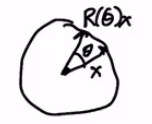
\includegraphics[width=5cm]{images/lec7-2.png}
    \caption{\textit{Givens rotation}}
\end{figure}

More generally, we will take components $i$ and $j$ of a vector and rotate them: \begin{align*}
    R(i,j,\theta) = \text{ identity except for rows and columns } i \text{ and } j, \text{ containing entries of }R(\theta)
\end{align*}
To do QR, we want to create zero entries. So given $x(i)$ and $x(j)$, we want $\theta$ so that $R(i,j,\theta)x$ is 0 in entry $j$: \begin{align*}
    \left[\begin{array}{cc}
        \cos \theta & -\sin \theta \\
        \sin \theta & \cos \theta
        \end{array}\right]\left[\begin{array}{l}
        x(i) \\
        x(j)
        \end{array}\right]=\left[\begin{array}{c}
        \sqrt{x(i)^{2}+x(j)^{2}} \\
        0
        \end{array}\right]
\end{align*}
or \begin{align*}
    &\cos \theta=\frac{x(i)}{\sqrt{x(i)^{2}+x(j)^{2}}}, \\
    &\sin \theta=\frac{-x(j)}{\sqrt{x(i)^{2}+x(j)^{2}}}
\end{align*}
We do QR by repeatedly multiplying $A$ by $R(i,j,\theta)$ matrices to introduce new zeros, until $A$ becomes upper triangular.
When $A$ is sparse, this may cause less fill-in than \textit{Householder transformations}.

\subsubsection{Stability of Applying Orthogonal Matrices}
Simple summary: Any algorithm that just works by multiplying an input matrix by orthogonal matrices is always backwards stable. 
This covers QR composition using \textit{Householder} or \textit{Givens rotations}, as well as later algorithms for the eigenproblem and SVD.

Here is why this is true: By using the basic rule $\operatorname{fl}(a \odot b) = (a \odot b)(1+\delta)$, $|\delta| \leq \varepsilon$, 
one can show that for either multiplying by one \textit{Householder} or \textit{Givens transformation} $Q$ one gets the following, 
where $Q^\prime$ is the floating point transformation actually stored in the machine, e.g. \begin{align*}
    Q^\prime = I - 2u^\prime u^{\prime \top}
\end{align*}where u' is the computed \textit{Householder} vector: \begin{align*}
    \operatorname{fl}(Q^\prime A) = Q^\prime A+E
\end{align*}
where $\norm{E} = O(\varepsilon) \norm{A}$ This follows from our earlier analysis of dot products, etc. As can be seen from the above formula for $u=\operatorname{House}(x)$, 
every component u'(i) is nearly equal to the exact value u(i), but roundoff keeps it from being perfect. Since $Q^\prime$ is nearly equal to the exact orthogonal $Q$, 
then $Q^\prime=Q+F$ with $\norm{F} = O(\varepsilon)$, so we can also write this as \begin{align*}
    \operatorname{fl}(Q^\prime A) = (Q+F)A + E = QA + (FA + E) = QA + G
\end{align*}
where $\norm{G} \leq \norm{F}\norm{A} + \norm{E} = O(\varepsilon)\norm{A}$. i.e. you get an exact orthogonal transformation $QA$ plus a small error. 
The same result applies to \textit{Givens rotations} and \textit{block Householder transformations} (used to reduce communication).
We can also write this as \begin{align*}
    \operatorname{fl}(Q^\prime A) = QA + G = Q(A+Q^\top G) = Q(A + F),
\end{align*}
where $\norm{F} = \norm{G} = \norm{f}=O(\varepsilon)\norm{A}$, i.e. multiplying by $Q$ is backward stable: 
we get the exact orthogonal transformation of a slightly different matrix $A+F$. Now multiply by a sequence of orthogonal matrices, as in QR decomposition: \begin{align*}
    \operatorname{fl}\left( Q^\prime_3 \left( Q^\prime_2 \left( Q^\prime_1 A \right) \right) \right) &= 
    \operatorname{fl}\left( Q^\prime_3 \left( Q^\prime_2 \left( Q_1 A + E_1 \right) \right) \right) \\
    &= \operatorname{fl}\left( Q^\prime_3 \left( Q_2 \left( Q_1 A + E_1 \right) + E_2 \right) \right) \\
    &= Q_3 \left( Q_2 \left( Q_1 A + E_1 \right) + E_2 \right) + E_3 \\
    &= Q_{3} Q_{2} Q_{1} A+Q_{3} Q_{2} E_{1}+Q_{3} E_{2}+E_{3} \\
    &= \left(Q_{3} Q_{2} Q_{1} A\right)+E \\
    &= \underbrace{Q_{3} Q_{2} Q_{1}}_{Q} \left(A+Q^{\top} E\right) \\
    &= Q(A+F)
\end{align*}
where \begin{align*}
    \norm{F} = \norm{E} &\leq \norm{Q_{3} Q_{2} E_{1}} + \norm{Q_{3} E_{2}} + \norm{E_{3}} \\
    &= \norm{E_{1}}  + \norm{E_{2}}  + \norm{E_{3}} \\ 
    &= O(\varepsilon) \norm{A}
\end{align*}
so multiplying by many orthogonal matrices is also backwards stable. This analysis explains not just why QR is stable, 
but also why computed $Q$ nearly orthogonal.

There is one more very simple, and fast, QR decomposition algorithm, called \textit{CholeskyQR}: \begin{algorithmfrm}[CholeskyQR]
    \begin{algorithmic}[1]
        \State Factor $A^\top A = R^\top R$ using \textit{Cholesky}
        \State $Q=AR^{-1}$
    \end{algorithmic}
\end{algorithmfrm}
It is clear that $QR = A$, and $Q^\top Q = R^{-\top}A^\top AR^{-1} = I$. But since we form $A^\top A$, this will clearly be unstable if $A$ is ill-conditioned, 
and fails completely if Cholesky fails to complete, which can happen if we need to take the square root of a nonpositive number 
(which also means the trick of running it twice, as used with Gram-Schmidt, doesn't work either).

\newpage
\section{Lecture 8: Low Rank Matrices}
Dealing with low rank (or nearly) matrices. Motivation: Real data is often low rank. So we want to
\begin{enumerate}
    \item Take precautions to avoid inaccuracy in Least Squares.
    \item Use it to compress data, go faster, both deterministically and using randomization.
\end{enumerate}
Use LS as an application of compression, but many others. 

\subsection{Solving an LS Problem when Matrix Rank Deficient}
\begin{theorem}
    Let $A$ be $m \times n, \ m \geq n, \ \operatorname{rank}A < n$. \begin{align*}
        A = U \Sigma V^{\top} = \left[ U_1, U_2, U_3 \right] \left[\begin{array}{ll}
            \Sigma_{1} & 0 \\
            0 & \Sigma_{2} \\
            0 & 0
            \end{array}\right] \left[ V_1, V_2 \right]
    \end{align*}
    Here $\Sigma_1$ is full rank, $\Sigma_2=0$. The set of vectors minimizing $\norm{Ax-b}_2$ is 
    
    $\left\{ x=V_1 \Sigma_1^{-1} U^\top_1 b + V_2 y_2, \ \forall y_2 \in \RR^{n-r}  \right\}$. The unique $x$ minimizing $\norm{Ax-b}_2$ and $\norm{x}_2$ is gotten by $y_2 = 0$:
    $$x=V_{1} \Sigma_{i}^{-1} U_{i}^{\top} b$$
\end{theorem}
\begin{definition}
    $A^{+} = V_{1} \Sigma_{1}^{-1} U_{1}^{\top}$ is Moore–Penrose pseudo inverse of $A$ (include full rank case $n=r$)
\end{definition}
So square or not, full rank or not, best solution $x=A^+ b$.
\begin{proof}
    \begin{align*}
        \norm{Ax-b}_2 &= \norm{U\Sigma V^\top x -b }_2 \\
        &= \norm{\Sigma V^\top x - U^\top b }_2 \\
        &= \norm{\Sigma y - U^\top b }_2 \\
    \end{align*}
    $y=V^\top x$ and $x$ have same norm. Since $V$ orthogonal, so finding LS minimizing $\norm{y}_2$ also minimizes the follows, \begin{align*}
        \norm{x}_2 &= \norm{\left[\begin{array}{l}
            \Sigma_1 y_{1}-U_{1}^{T} b \\
            \Sigma_2 y_{1}-U_{2}^{T} b \\
            \Sigma_3 y_{1}-U_{3}^{T} b 
            \end{array}\right]}_2
    \end{align*}
    where $y=\left[\begin{array}{l}
        y_{1} \\
        y_{2}
        \end{array}\right]$ minimized by $y_1=\Sigma^{-1}Y_1^\top b$ and $\sqnorm{y}=\sqnorm{y_1} + \sqnorm{y_2}$ minimized by $y_2=0$.\begin{align*}
            x &= Vy \\
            &= V_1 y_1 + V_2 y_2 \\
            &= V_1 y_1 \\
            &= V_1 \Sigma^{-1}Y_1^\top b
        \end{align*}
\end{proof}

\subsection{Solving LS when Matrix nearly Rank Deficient with Truncated SVD}
We have defined the condition number of a matrix $\kappa(A)$ as $\frac{\sigma_{\operatorname{max}}} {\sigma_{\operatorname{min}}}$, 
where $\sigma_{\operatorname{min}}=0$ if for a rank deficient matrix, so the condition number is formally infinite.
\begin{example}
    Considering
    \begin{align*}
        \arg \min \| \left[\begin{array}{ll}
            1 & 0 \\
            0 & 0 \\
            0 & 0
            \end{array}\right] \left[\begin{array}{l}
                x_{1} \\
                x_{2}
                \end{array}\right] - \left[\begin{array}{l}
                    1 \\
                    1 \\
                    1
                    \end{array}\right] \|_2 = \left[\begin{array}{l}
                        1 \\
                        0
                        \end{array}\right]
    \end{align*}
    and 
    \begin{align*}
        \arg \min \| \left[\begin{array}{ll}
            1 & 0 \\
            0 & e \\
            0 & 0
            \end{array}\right] \left[\begin{array}{l}
                x_{1} \\
                x_{2}
                \end{array}\right] - \left[\begin{array}{l}
                    1 \\
                    1 \\
                    1
                    \end{array}\right] \|_2 = \left[\begin{array}{l}
                        1 \\
                        0
                        \end{array}\right]
    \end{align*}
    The solutions are arbitrarily different as $e \rightarrow 0$.
\end{example}
What does a solution mean if it can change discontinuously? Often $A$ is not known exactly. Just up to some tolerance $\norm{A - A^\prime \leq t_0}$. If $A$ nearly singular, what do you do?

\begin{definition}[Truncated SVD]
    If $A=U \Sigma V^{\top}$ is SVD of $A$, then, 
    $$A(\text{tol})=U\Sigma (\text{tol})V^\top$$ 
    where  $\Sigma (\text{tol})=\operatorname{diag}\left( \sigma_1 (\text{tol}),\sigma_2 (\text{tol}), \cdots, \sigma_n (\text{tol}) \right)$, 
    $$\sigma_{i}\left(t_{0} 1\right)=\left\{\begin{array}{l}
        \sigma_{i} \ \text{if } \sigma_i \geq \text{tol} \\
        0 \ \text{if } \sigma_i < \text{tol} \\
        \end{array}\right.$$
    i.e. we truncate small singular values to 0. Or, we replace $A$ by lowest rank matrix $A(\text{tol})$ within distance tol. Using $A(\text{tol})$ for LS effectively reduces
    $k=\frac{\sigma_{\operatorname{max}}} {\sigma_{\operatorname{min}}}$ to $\frac{\sigma_{\operatorname{max}}}{\mathrm{tol}}$. Tol is a knob  that user can pick to trade off sensitivity and how well $B$ can be approximated by 
    $A(\mathrm{tol})x$, because $\operatorname{span}(A(\mathrm{tol}))$ decreases as $\mathrm{tol}$ increases. Replacing $A$ by an easier matrix also called regularization, several mechanisms.
\end{definition}

Using the truncated SVD effectively replaces the usual condition number
$\frac{\sigma_{\operatorname{max}(A)}}{\sigma_{\operatorname{min}(A)}}$ by $\frac{\sigma_{\operatorname{max}(A)}}{\mathrm{tol}}$, which can be much smaller, 
depending on the choice of $\mathrm{tol}$. In other words, $\mathrm{tol}$ is a "knob" one can turn to trade off conditioning with how closely $Ax$
can approximate $b$ (raising $\mathrm{tol}$, and so lowering the rank of $A$, decreases the dimension of the space that can be approximated by $Ax$).

Replacing $A$ by an "easier" matrix is also called "regularization" (using the truncated SVD is just one of several mechanisms). 
The following Lemma illustrates this in a special case, where just vector $b$ changes. 
The general case depends on whether one picks tol in a "gap" between singular values, 
since otherwise a small perturbation could change the number of singular values is greater than $\mathrm{tol}$.

\begin{lemma}
    The difference between \begin{align*}
        x_1 = \underset{x}{\arg \min} \norm{A(\mathrm{tol})x - b_1}_2
    \end{align*}
    and
    \begin{align*}
        x_2 = \underset{x}{\arg \min} \norm{A(\mathrm{tol})x - b_2}_2 
    \end{align*}
    where we choose the solution of smallest norm in both cases, is bounded by $\norm{b_1 - b_2}_2 / \mathrm{tol}$, i.e. \begin{align*}
        \norm{x_1 - x_2}_2 \leq \frac{\norm{b_1 - b_2}}{\mathrm{tol}}
    \end{align*}
    So choosing a larger $\mathrm{tol}$ limits the sensitivity of the solution.
    \begin{proof}
        Let $A = U\Sigma V^\top$ and $A(\mathrm{tol}) = U\Sigma(\mathrm{tol})V^\top$ as above. Then \begin{align*}
            \left\|x_{1}-x_{2}\right\|_{2} &= \norm{A(\mathrm{tol})^{+} (b_1-b_2)}_2 \\
            &= \norm{V(\Sigma(\mathrm{tol}))^{+} U^\top (b_1 - b_2)}_2 \\
            &= \norm{\operatorname{diag}\left( 1/\sigma_1,1/\sigma_2, \cdots, 1/\sigma_k, 0, \cdots \right) U^\top (b_1-b_2)}
        \end{align*}
        where $\sigma_k \geq \mathrm{tol}$, \begin{align*}
            &\leq \frac{1}{\sigma_k} \norm{U^\top (b_1-b_2}_2 \\
            &= \frac{1}{\sigma_k} \norm{(b_1-b_2}_2 \\
            &\leq \frac{1}{\mathrm{tol}} \norm{(b_1-b_2}_2 \\
         \end{align*}
    \end{proof}
\end{lemma}

So that tells us that increasing the tolerance lowers the sensitivity. So we can also analyze the effect of changing $A$ on $A(\mathrm{tol})$ 
depends on whether the rank of $A(\mathrm{tol})$ changes. And so you need to assume that it doesn't get continuity, which means $\mathrm{tol}$ can't be closed 
to an existing singular value. Because otherwise changing the matrix slightly could make $\sigma_i$ cross the threshold of tolerance and change the rank.

Setting small singular values to zero also compresses the matrix, since it costs
just $(mk + k + kn)$ numbers to store, as opposed to $mn$. So $\mathrm{tol}$ is also a "knob" that trades off compression with approximation accuracy.

The SVD is the most precise and most accurate way to approximate a matrix by one of lower rank, costing $O(mn^2)$, with a big constant. 
Now we explore other cheaper ones, both deterministic and randomized.

\subsection{Solving a Least Squares Problem when A is (nearly) Rank Deficient}
\subsubsection{With Ridge Regression}
Another common way to deal with the drawback of the solution becoming unbounded as the smallest singular values of $A$ approach 0, is regularization, or computing
\begin{align*}
    x &= \underset{x}{\arg \min}\sqnorm{Ax-b} + \lambda^2 \sqnorm{x} \\
    &= \underset{x}{\arg \min}\sqnorm{\left[\begin{array}{c}
        A \\
        \lambda I
        \end{array}\right]^{x}-\left[\begin{array}{l}
        b \\
        0
        \end{array}\right]}
\end{align*}
where $\lambda$ is a "tuning parameter" to be chosen by the user. The larger $\lambda$ is chosen, the more weight is placed on $\norm{x}_2$, 
so the more important it is to minimize relative to $\norm{Ax-b}_2$.

We can easily write down the normal equations: \begin{align*}
    x=\left(A^{\top} A+\lambda^{2} I\right)^{-1} A^{\top} b
\end{align*}
Adding $\lambda^2$ to the diagonal of $A^\top A$ before Cholesky just increases all the eigenvalues of $A^\top A$ by $\lambda^2$, pushing it farther away from being singular.
If $A = U\Sigma V^\top$ is the thin SVD of $A$, then substituting this for $A$ yields \begin{align*}
    x &= V(\Sigma (\Sigma^2 + \lambda^2 I)^{-1} ) U^{\top} b \\
    &= V \operatorname{diag}\left( \frac{\sigma_i}{\sigma_i^2 + \lambda^2} \right)U^{\top} b 
\end{align*}
which reduces to the usual solution when $\lambda = 0$. Note that when $\sigma_i \gg \lambda$, the above expression is close to $\frac{1}{\sigma_i}$ as expected,
and when $\sigma_i < \lambda$, it is bounded by $\frac{\sigma_i}{\lambda^2}$, so it can't get larger than $\frac{1}{\lambda}$. 
Thus $\lambda$ and $\mathrm{tol}$ in $A(\mathrm{tol})$ play similar roles.

\subsubsection{With QR Decomposition}
Our next alternative to the truncated SVD is QR with column pivoting. Suppose we did $A = QR$ exactly, with $\operatorname{rank}(A)=r<n$, what would $R$ look like?
If the leading $r$ columns of $A$ were full rank (true for "most" such $A$), then \begin{align*}
    R=\left[\begin{array}{ll}
        R_{11} & R_{12} \\
        0 & R_{22}
        \end{array}\right]
\end{align*}
with $R_{11}$ is $r \times r$ and full rank, so $R_{22}$ to zero. If $A$ is nearly low-rank, we can hope that $\norm{R_{22}} < \mathrm{tol}$,
and set $R_{22}$ to zero. Assuming that this works for a moment, write \begin{align*}
    A=Q R=\left[Q, Q^{\prime}\right]\left[\begin{array}{l}
        R \\
        0
        \end{array}\right],
\end{align*}
with $\left[Q, Q^{\prime}\right] = \left[Q_1, Q_2, Q^{\prime}\right]$ square and orthogonal as before, with $Q_1$ $m \times r$, $Q_2$ $m \times (n-r)$ and $Q^\prime$ $m \times (m-n)$.
Thus \begin{align*}
    \underset{x}{\arg \min}\norm{Ax-b}_2 &= \underset{x}{\arg \min}\norm{\left[Q_1, Q_2, Q^{\prime}\right]\left[\begin{array}{l}
        R \\
        0
        \end{array}\right]x-b}_2 \\
        &= \underset{x}{\arg \min}\norm{\left[\begin{array}{rl}
            R_{11} x_{1}+R_{12} x_{2} & -Q_{1}^{T} b \\
            & -Q_{2}^{\top} b \\
            & -Q^{\prime} b
            \end{array}\right]}_2
\end{align*}

How do we pick $x_2$ to minimize $\norm{x}_2$?
\begin{example}
    $A=\left[\begin{array}{ll}
        e & 1 \\
        0 & 0
        \end{array}\right]=\left[\begin{array}{ll}
        R_{11} & R_{12} \\
        0 & R_{22}
        \end{array}\right]$, $b=\left[\begin{array}{l}
            b_{1} \\
            b_{2}
            \end{array}\right]$, $x=\left[\begin{array}{c}
                \left(b_{1}-x_{2}\right) \\
                x_{2}
                \end{array}\right]$.
    And so if $e$ is tiny, we better pick $x_2$ carefully (close to $b_1$) to keep $\norm{x}$ small. But if we permute the columns of $A$ to $AP$ and minimize
    $\norm{AP \hat{x} - b}_2$ we get \begin{align*}
        A P=\left[\begin{array}{ll}
            1 & e \\
            0 & 0
            \end{array}\right]=\left[\begin{array}{ll}
            R_{11} & R_{12} \\
            0 & R_{22}
            \end{array}\right].
    \end{align*}
    Thus \begin{align*}
        x=\left[\begin{array}{c}
            b_{1}-e x_{2} \\
            x_{2}
            \end{array}\right]
    \end{align*}
    So $\norm{x}$ is much less sensitive to the choice of $x_{2}$. 
\end{example}

What would a "perfect" $R$ factor look like? We know the SVD gives us the best possible
answer, so comparing $\left[\begin{array}{ll}
    R_{11} & R_{12} \\
    0 & R_{22}
    \end{array}\right]$ to $\left[\begin{array}{cc}
        \Sigma_{1} & 0 \\
        0 & \Sigma_{2}
        \end{array}\right]$ makes sense. These observations motivate the following (\textbf{INFORMAL}) definition.

\begin{definition}
    A Rank Revealing QR Factorization (\textit{RRQR}) of $A$ is $AP = QR$ where $P$ is a permutation, $Q$ orthogonal, $R=\left[\begin{array}{ll}
        R_{11} & R_{12} \\
        0 & R_{22}
        \end{array}\right]$ with $R_{11}$ $k \times k$ where \begin{enumerate}
            \item $R_{22}$ is "small", ideally $\sigma_{\mathrm{max}}(R_{22}) = O(\sigma_{k+1}(A))$, i.e. $R_{22}$ "contains" the $n-k$ smallest singular values of $A$
            \item $R_{11}$ is "large", ideally $\sigma_{\mathrm{min}}(R_{11})$ not much smaller than $\sigma_{k}(A)$
            \item[] \textit{If in additional to the above two, we have:}
            \item $\norm{R_{11}^{-1}R_{12}}$ is "not too large", then we call $AP = QR$ a "strong rank revealing QR"
        \end{enumerate}
\end{definition}

\begin{theorem}[\textbf{INFORMAL}]
    If the above 3 statements hold, then for $i=1:k$, \begin{align*}
        \sigma_{i}(A) \geq \sigma_{i}(R_{11}) \geq \frac{\sigma_{i}(A)}{\sqrt{1 + \sqnorm{R_{11}^{-1}R_{12}}}},
    \end{align*}
    and for $i=k+1:n$, \begin{align*}
        \sigma_{i}(A) \leq \sigma_{\mathrm{max}}(R_{22}) \sqrt{1 + \sqnorm{R_{11}^{-1}R_{12}}}
    \end{align*}
\end{theorem}

In other words, the singular values of $R_{11}$ are good approximations of the largest $k$ singular values of $A$, 
and the smallest $n-k$ singular values of $A$ are roughly bounded by $\norm{R_{22}}$. Or, the leading $k$ columns of $AP$
contain most of the information of the range space of $A$: \begin{align*}
    AP &= \left[ A_1, A_2 \right] = QR = \left[ Q_1, Q_2 \right]\left[\begin{array}{ll}
        R_{11} & R_{12} \\
        0 & R_{22}
        \end{array}\right] \\
    &\approxeq \left[ Q_1, Q_2 \right]\left[\begin{array}{ll}
        R_{11} & R_{12} \\
        0 & 0
        \end{array}\right] \\
    &= Q_1 R_{11} \left[ I, R_{11}^{-1}R_{12} \right] \\
    &= A_1  \left[ I, R_{11}^{-1}R_{12} \right]
\end{align*}

\subsection{Computer the Permutation}
\subsubsection{QR with Column Pivoting}
\textit{QRCP} is the oldest and simplest way, and often works, but like LU with partial pivoting, there are some rare matrices where it fails by a factor near $2^n$. 
And it maximizes communication. At the first step, the algorithm chooses the column of $A$ of largest norm;
at each following step, the algorithm picks the column with the biggest component orthogonal to all the columns already chosen.
Intuitively, this "greedy algorithm" picks the column with the biggest projection in a direction not spanned by previously chosen columns.
The algorithm is simply
\begin{algorithmfrm}[QRCP]
    \begin{algorithmic}
        \For{$i=1:\min(m-1,n)$ or or until the trailing submatrix ($R_22$) is small enough}
        \State Choose largest column in trailing matrix, i.e. $\underset{j \geq i}{\arg \max} \norm{A(i:m,j)}$
        \If{$i \neq j$}
            \State Swap columns $i$ and $j$
        \EndIf
        \State Multiply $A(i:m,i:n)$ by a \textit{Householder reflection} to zero out $A(i+1:m,i)$
        \EndFor
    \end{algorithmic}
\end{algorithmfrm}

If the algorithm stops after $k$ steps, because the trailing matrix $A(k+1:m,k+1:n)$ has no column larger than some tolerance, the cost is about $4mnk$, 
versus $O(mn^2)$ for the SVD, so much cheaper if $k \sim \operatorname{rank}(A) \ll n$.

To understand why this works: the first multiplication by a Householder reflection decomposes trailing columns into a part parallel to first column 
(now just parallel to $e_1$) and an orthogonal part (in rows $2:m$). Choosing the column of biggest norm in rows $2:m$ chooses the column with the biggest
component orthogonal to the first column.

At each step we similarly choose the trailing column with the biggest component orthogonal to the previously chosen columns.
The arithmetic cost is low, since we can just update $\norm{A(i:m,j)}$ from iteration to iteration for O(m*n) cost, rather than recomputing them for $O(mn^2)$ cost.
But this simple algorithm "maximizes communication", since we read and write the entire trailing matrix $A(i:m,i:n)$ at each step. 
This is available in \textit{LAPACK} \textit{geqpf} and \textit{MATLAB} \texttt{[Q,R,P]=qr(A)}.

Here is a typical example, which shows how well each $R(i,i)$ approximates $\sigma_i$:
\begin{minted}{matlab}
    A = randn(50)*diag(.5.^(1:50))*randn(50);[Q,R,P]=qr(A);r=abs(diag(R));s=svd(A);
    figure(1),semilogy(1:50,r,'r',1:50,s,'k'),title('red = diag(r), black = svd')
    figure(2),plot(r./s),title('diag(r)/svd'), figure(3), spy(P)
\end{minted}


As a (rare) example where \textit{QRCP} fails to pivot well, consider $A = SCD$ where
\begin{minted}{matlab}
    cs = 1/sqrt(2); sn = 1/sqrt(2); n=30;
    S = diag(sn.^(0:n-1)); C = eye(n)-cs*triu(ones(n,n),1); D = diag(.9999.^(0:n-1));
    A = S*C*D; [Q,R,P]=qr(A);figure(2),spy(P);pause, r=abs(diag(R));s=svd(A);
    figure(1),semilogy(1:n,r,'r+-',1:n,s,'k+-'),title('red = diag(R), black = svd')
    figure(3),semilogy(1:n,r./s,'k+-'), title('diag(r)/svd')
\end{minted}

i.e. $C$ has ones on the diagonal and $-cs$ above the diagonal. $sn$ and $cs$ satisfy $sn^2+cs^2=1$. $D$ is not necessary in exact arithmetic, 
but avoids roundoff problems. $A$ is upper triangular, and \textit{QRCP} does not permute any columns, so $A = QR = IA$.
Letting $k=n-1$ yields $R_{22} = sn^(n-1)$ but \begin{align*}
    \sigma_n (A) &= \frac{1}{\norm{A^{-1}}} \sim \frac{1}{\norm{C^{-1}S^{-1}}} \leq \frac{1}{\norm{C^{-1}(:,n)sn^{1-n}}} \\
    &< \frac{sn^{1-n}}{cs(1+cs)^{n-2}}
\end{align*}
So $\sigma_n(A)$ can be smaller than $R_{22}$ by an exponentially large factor $cs(1+cs)^(n-2)$, which can grow as fast as $2^(n-2)$ when $cs \sim 1$.
So \textit{QRCP} has two weaknesses: (rare) failure to pivot well, and high communication cost. We address these in turn.

\subsection{Fixing Pivoting for QR}
\subsubsection{Gu/Eisentat Strong RRQR Algorithm}
This algorithm deals with the rare failure to pivot correctly. It uses a more complicated pivoting scheme, that depends on the norms of columns of $R_{22}$, 
rows of $R_{11}^{-1}$, and entries of $R_{11}^{-1}R_{12}$, and guarantees a strong \textit{RRQR}. It does so by cheaply exchanging a column in $R_{11}$ 
and another column not in $R_{11}$ if that increases $\operatorname{det}(R_{11})$ by a sufficient factor.
It still costs only $4mnk$ (plus lower order terms), about the same as \textit{QRCP} when $m \gg n$.

\subsubsection{Avoiding Communication in QR with Column Pivoting}
Neither of the last two algorithms was designed with minimizing communication in mind, 
and so both access the entire matrix each time a column is chosen, and so the number of read/writes is also $O(mn^2)$,
same as the number of flops, instead of the hoped for factor of $\sqrt{\mathrm{fast\_memory\_size}}$ smaller. 

The first attempt to fix this is in \textit{LAPACK} \textit{geqp3.f}. This uses matrix multiply to update the trailing submatrix, 
as do LU and plain QR, but only reduces the number of reads/writes by two times compared to the simple routine. Still, it is often faster.

But to approach the lower bound, we seem to need a different pivoting strategy, which can choose multiple pivot columns for each matrix access, not just 1.
The approach is similar to the \textit{TSLU} algorithm described earlier. We present the sequential version, 
which chooses $b$ pivot columns with one pass through the matrix (the parallel version is analogous). $b$ is a blocksize to be chosen for accuracy/performance.

\begin{savenotes}
    \begin{algorithmfrm}
        \begin{algorithmic}
            \State $\mathrm{BestColumnsSoFar}=(1:b)$
            \For{$k=b+1:n-b+1:b$}\Comment{Assume $b | n$ for simplicity}
            \State Form $m \times 2b$ matrix $A_{2b}$ from columns in $\mathrm{BestColumnsSoFar}$ and columns $k:k+b-1$
            \State Choose the $b$ "best columns" among the $2b$ columns in $A_{2b}$\footnote{For example by: factor $A_{2b}=QR$, using \textit{TSQR}. Choose best $b$ columns of $R$ (just $2b \times 2b$), using \textit{RRQR} or \textit{Strong RRQR}, update BestColumnsSoFar based on result.}
            \EndFor
        \end{algorithmic}
    \end{algorithmfrm}
\end{savenotes}

After each outer iteration, $\mathrm{BestColumnsSoFar}$ contains the indices of the $b$ best columns found so far among columns $1$ to $k+b-1$. 
The parallel version takes pairs of $m \times b$ submatrices, chooses the best $b$ columns from each set of $2b$, 
and proceeds to pair these up and choose the best (which is why we call it "tournament pivoting" by analogy to having a "tournament" where at each round
we choose the best). However, the flop count roughly doubles compared to \textit{QRCP}.

\subsection{Low Rank Factorization without Orthogonality}
So far we have only considered low rank factorizations where (at least) one factor is an orthogonal matrix, say $Q$ in $QR$. 
$Q$ can be thought of as linear combinations of columns of $A$, which approximate the column space of $A$. 
But not all data analysis questions can best be answered by such linear combinations. Suppose the rows represent individual people, 
and the columns represent some of their characteristics, like age, height and income. If one of the columns of $Q$ happens to be \begin{align*}
    .2\mathrm{age} - .3\mathrm{height} + .1\mathrm{income} + \cdots
\end{align*}
then it can be hard to interpret what this means, as a "predictor" of the other columns/characteristics, like "been treated for disease X". 
And if there are thousands of columns, it is even harder. Instead, it would be good to be able to approximate the other columns by linear combinations of as few columns as possible,
and analogously to approximate the other rows by a subset of the rows. This leads to the following decomposition.

\begin{definition}
    A CUR decomposition of a matrix $A$ is consists of the matrices:\begin{itemize}
        \item $C$ is a subset of $k$ columns of $A$
        \item $R$ is a subset of $k$ rows of $A$
        \item $U$ is a $k \times k$ matrix
    \end{itemize}
    where $\norm{A - CUR}$ is "small", i.e. close to the lower bound $\sigma_{k+1}$, which is attained by the SVD truncated to rank $k$.
\end{definition}

A number of algorithms for computing a CUR decomposition have developed over time, see the class webpage for details. Here we highlight two, 
because they are easy to implement given the tools we have already presented: \begin{enumerate}
    \item Perform QR with some kind of column pivoting, to pick the $k$ "most linearly independent" columns of $A$; 
    let $J = [j_1, j_2, \cdots , j_k]$ be the indices of these columns, and let $C$ consist of these columns of $A$.
    \item Perform \textit{GEPP}, or \textit{TSLU}, on $C$, to pick the $k$ most linearly independent rows of $C$; 
    let $I = [i_1, i_2, \cdots , i_k]$ be the indices of these rows, and let $R$ consist of these rows of $A$.
\end{enumerate}
Having chosen $C$ and $R$, we still need to choose $U$ so that $CUR$ approximates $A$.
Here are two approaches: \begin{enumerate}
    \item The best possible $U$ is given by the solution to HW 3.12: the $U$ that minimizes the Frobenious norm of $A - CUR$ is $U=C^{+}AR^{+}$.
    \item A cheaper approximation is just to choose $U$ so that $CUR$ equals $A$ in columns $J$ and rows $I$. 
    Since the 3 $k$-by-$k$ matrices $C(I,1:k) = R(1:k,J) = A(I,J)$ are equal, we just let $U$ be the inverse of this common matrix.
\end{enumerate}

\subsection{Randomized Linear Algebra}
Now we consider randomized algorithms. Related reading is posted on the \href{https://people.eecs.berkeley.edu/~demmel/ma221_Fall20/}{class webpage}. 
The basic idea for many randomized algorithms is as follows: Let $Q$ be an $m \times k$ random orthogonal matrix, with $k \ll n$. 
Then we approximate $A$ by $Q\left(Q^{\top} A\right)$, the projection of $A$'s columns onto the space spanned by $Q$. 
Since $Q\left(Q^{\top} A\right)$ has $k \ll n$ columns, solving the LS problem is much cheaper than with $A$.
Multiplying $Q^\top A$ costs $2mnk$ flops if done straightforwardly, which is only about 2 times cheaper than \textit{QRCP} above. 
So there has been significant work on finding structured or sparse $Q$, and not necessarily orthogonal, to make computing $Q^\top A$ much cheaper. 
To date the best (and surprising result) says that you can solve a LS problem approximately, where A is sparse, with just $O(\operatorname{nnz}(A))$ flops,
where $\operatorname{nnz}(A)$ is the number of nonzeros in $A$.

We give some motivation for why such a random projection should work by some low-dimensional examples, and then state the \textit{Johnson-Lindenstrauss Lemma},
a main result in this area.

\begin{example}
    Suppose $x$ is a vector in $\RR^2$, and $q$ is a random unit vector in $\RR^2$, i.e. $q = [\sin t, \cos t]^\top$ where $t$ is uniformly distributed on $[0,2\pi)$. 
    What is the distribution of \begin{align*}
        |x^\top q|^2 = (\norm{x} |\cos(\angle(x,q))|)^2
    \end{align*}
    It is easy to see that $\angle(x,q)$ is also uniformly distributed on $[0,2\pi)$, so the expected value is \begin{align*}
        \EE(|x^\top q|^2) = .5 \norm{x}^2,
    \end{align*} 
    and more importantly, the probability that $|x^\top q|^2$ underestimates $\norm{x}^2$ by a tiny factor $e$, 
    is $P(|\cos(t))|^2 < e) \sim 2\sqrt{e}/\pi$, so tiny too.
\end{example}

\begin{example}
    Now suppose $x$ is a vector in $\RR^3$, and $Q$ represents a random plane, i.e. $Q$ is a random $3\times 2$ orthogonal matrix, 
    and $x^\top Q$ is the projection of $x$ onto the plane of $Q$. We again ask how well the size of the projection $\norm{x^\top Q}^2$ approximates $\norm{x}^2$.

    Now the probability that $\norm{x^\top Q}^2<e\norm{x}^2$ is the same as the probability that $x$ is nearly parallel to the perpendicular to the plane of $Q$, 
    which can be thought of as a random point on the unit sphere in $\RR^3$. This probability is $O(e)$, much tinier, 
    because $x$ needs to be nearly orthogonal to both columns of $Q$.

    Intuitively, as the number of columns of $Q$ increases, the chance that $\norm{x^\top Q}^2$ greatly underestimates $\norm{x}^2$ decreases rapidly. 
    The \textit{Johnson-Lindenstrauss Lemma} captures this, not just for one vector $x$, but for many vectors.
\end{example}

\begin{lemma}[Johnson-Lindenstrauss Lemma]
    Let $0< \varepsilon < 1$, and $x_1,\cdots, x_n$ be any $n$ vectors in $\RR^m$, and $k \geq 8\ln(n)/\varepsilon^2$.
    Let $F$ be a random $k \times m$ orthogonal matrix multiplied by $\sqrt{m/k}$. Then with probability at least $1/n$, for all $1 \leq i$, $j \leq n$, $i \neq j$,
    \begin{align*}
        1 - \varepsilon \leq \norm{F(x_i - x_j)}^2/\norm{x_i - x_j}^2 \leq 1 + \varepsilon
    \end{align*}
\end{lemma}

The point is that for $Fx$ to be an $\varepsilon$ approximation of $x$ in norm, the number of rows of $F$ grows "slowly", 
proportional to $\ln(n) = \ln(\#\mathrm{vectors})$ and $1/\varepsilon^2$. The probability $1/n$ seems small, but being positive it means that $F$ exists
(the original goal of Johnson and Lindenstrauss). And it comes from showing that the probability of a large error for any one vector $x_i - x_j$ is tiny, 
just $2/n^2$. This justifies using a single random $F$ in the algorithms below.

(The proof follows by observing that we can think of $F$ as fixed and each vector $x=x_i - x_j$ as random, 
and simply take $F$ as the first $k$ rows of the mxm identity, and each entry of $x$ an i.i.d. (independent, identically distributed) Gaussian $\mathcal{N}(0,1)$,
i.e. with 0 mean and unit standard deviation, reducing the problem to reasoning about sums of squares of i.i.d. $\mathcal{N}(0,1)$ variables. 
See \href{http://cseweb.ucsd.edu/~dasgupta/papers/jl.pdf}{An Elementary Proof of a Theorem of Johnson and Lindenstrauss} for details.

There is a range of different $F$ matrices that can be used, which tradeoff cost and statistical guarantees, and are useful in different applications.
\footnote{See \href{https://arxiv.org/abs/2002.01387}{Randomized Numerical Linear Algebra: Foundations and Algorithms} and \href{http://arxiv.org/abs/0909.4061}{Finding Structure with Randomness: Probabilistic Algorithms for Constructing Approximate Matrix Decompositions} for surveys.}

One can construct a random orthogonal $m \times k$ matrix $Q$, with $m \geq k$, simply as follows:
Let $A$ be $m \times k$, with each entry i.i.d. $\mathcal{N}(0,1)$, and factor $A = QR$. Then $F = \sqrt{\frac{m}{k}} Q$ in the J-L Lemma.
But this costs $O(mk^2)$ to form $F$, which is too expensive in general.

In some applications, it is enough to let each entry of $F$ be i.i.d. $\mathcal{N}(0,1)$, without doing QR until later in the algorithm, 
we will see an example of this below.  But multiplying $Fx$ still costs $O(mk)$ flops, when $x$ is dense.

The next alternative is the \textit{subsampled randomized Fourier Transform} (\textit{SRFFT}), for which $Fx$ only costs $O(m\log(m))$ or even $O(m\log(k))$. 
In this case $F = R \mathrm{FFT} D$ where $D$ is $m \times m$ diagonal with entries uniformly distributed on the unit circle in the complex plane,
$\mathrm{FFT}$ is the $m \times m$ \textit{Fast Fourier Transform}, $R$ is $k \times m$, a random subset of $k$ rows of the $m \times m$ identity.
There are also variations in the real case where the FFT is replaced by an even cheaper real (scaled) orthogonal matrix, the \textit{Hadamard transform}, 
all of whose entries are $\pm 1$, and $D$'s diagonal is also $\pm 1$; this is called \textit{SRHT}. The only randomness is in $D$ and $R$.
The intuition for why this works is that multiplying by $D$ and then the FFT "mixes" the entries of $x$ sufficiently randomly that sampling $k$ of them (multiplying by $R$) is good enough.

Finally, when $x$ is sparse, we would ideally like an algorithm whose cost only grew proportionally to $\operatorname{nnz}(x)$. In the real case, 
we can take $F = SD$ where $D$ is $m \times m$ diagonal with entries randomly $\pm 1$ (analogous to above), $S$ is $k \times m$, 
where each column is a randomly chosen column of the $k \times k$ identity. Note that $S$ and $R$ above are similar, but not the same. 
Multiplying $y = SDx$ can be interpreted as initializing $y=0$ and then adding or subtracting each entry of $x$ to a randomly selected entry of $y$. 
If $x$ is sparse, the cost is $\operatorname{nnz}(x)$ additions or subtractions. This is called Randomized Sparse Embedding in the literature.
This $F$ is not as "statistically strong" as the $F$'s described above, so we may need to choose a larger $k$ to prove any approximation properties.

\subsection{Apply to Least Squares}
Consider the dense least squares problem $x_{\mathrm{true}} = \underset{x}{\arg\min}\norm{Ax-b}_2$ where $A$ is $m \times n$ and $m \geq n$. 
We approximate this by \begin{align*}
    x_{\mathrm{approx}} = \underset{x}{\arg\min} \norm{F(Ax-b)}_2 = \underset{x}{\arg\min}\norm{(FA)x - Fb}_2.
\end{align*}

Using results based on the J-L Lemma, we can take $F$ to have $k = n\log(n)/\varepsilon^2$ rows in order to get \begin{align*}
    \norm{Ax_{\mathrm{approx}} - b}_2 \leq (1+\varepsilon)\norm{Ax_{\mathrm{true}} - b}_2,
\end{align*} 
in other words the residual is nearly as small as the true residual with high probability. 
But there is no guarantee about how far apart $x_{\mathrm{true}}$ and $x_{\mathrm{approx}}$ are.

Now we consider the cost. Given a dense $F$, forming $FA$ using dense matrix multiplication costs \begin{align*}
    O(kmn) = O(mn^2\log(n)/\varepsilon^2),
\end{align*}
so more than solving the original problem using QR, $O(mn^2)$. If we use \textit{SRFFT} or \textit{SRHT} and $A$ is dense, forming $FA$ costs just \begin{align*}
    O(mn\log(m)).
\end{align*}

Next, $FA$ has dimension $k \times n$ and so solving using QR costs $O(kn^2) = O(n^3 \log(n)/\varepsilon^2)$, for a total cost of \begin{align*}
    O(mn\log(m) + n^3\log(n)/\varepsilon^2),
\end{align*}
potentially much less than $O(mn^2)$ when $m \gg n$ and $\varepsilon$ is not too small. In other words, if high accuracy is needed ($\varepsilon$ is tiny),
a randomized algorithm like this may not help.

Finally, we mention a least squares algorithm that costs just just $O(\operatorname{nnz}(A))$, plus lower order terms. 
\footnote{For details see \href{https://dl.acm.org/doi/pdf/10.1145/3019134}{Low Rank Approximation and Regression in Input Sparsity Time} and 
\href{https://dl.acm.org/doi/pdf/10.1145/2488608.2488621}{Low-distortion Subspace Embeddings in Input-sparsity Time and Applications to Robust Linear Regression}.}
This uses the $F$ called a \textit{Randomized Sparse Embedding} above, with \begin{align*}
    k = O((n/\varepsilon)^2*log^6(n/\varepsilon))
\end{align*}
Then forming $FA$ and $Fb$ costs $\operatorname{nnz}(A)$ and $\operatorname{nnz}(b)$ respectively, much less than \textit{SRFFT} when $A$ is sparse. 
But note that $k$ grows proportionally to $n^2$, much faster than with the \textit{SRFFT}, where $k=O(n)$. 
If we solved \begin{align*}
    \underset{x}{\arg\min} \norm{(FA)x - Fb}_2
\end{align*} using dense QR, that would cost \begin{align*}
    O(kn^2) = O(n^4\log^6(n/\varepsilon)/\varepsilon^2),
\end{align*}
which is much larger than with \textit{SRFFT}. So instead we use a randomized algorithm again (say \textit{SRFFT}) to solve the problem.

\begin{theorem}
    With probability at least $2/3$, \begin{align*}
        \norm{A x_{\mathrm{approx}} - b}_2 \leq (1+\varepsilon)\norm{Ax_{\mathrm{true}} - b}_2
    \end{align*}
\end{theorem}

How can we make the probability of getting a good answer much closer to 1? Just run the algorithm repeatedly: After $s$ iterations, 
the probability that at least one iteration will have a small error rises to $1 - (1/3)^s$, and of the $s$ answers $x_1, \cdots, x_s$, 
the one that minimizes $\norm{Ax_i-b}_2$ is obviously the best one.

\subsection{Randomized Algorithms for Low Rank Factorizations}
Next we consider the problem of using a randomized algorithm for computing a low rank factorization of the $m \times n$ matrix $A$, with $m \geq n$.
We assume we know the target rank $k$, but since we often don't know $k$ accurately in practice, 
we will often choose a few more columns $k+p$ to see if a little larger (or smaller) $k$ is more accurate.

This algorithm is of most interest when $k \ll n$, i.e. the matrix is low rank. Note that in the following, the $F$ matrices will be tall-and-skinny, 
and applied on the right (e.g. $AF$), so the transpose of the cases so far.

\subsubsection{Randomized Low-Rank Factorization}
\begin{enumerate}
    \item Choose a random $n(k+p)$ matrix $F$.
    \item Form $Y = AF$, which is $m(k+p)$, we expect $Y$ to accurately span the column space of $A$.
    \item Factor $Y = QR$, so $Q$ also accurately spans the column space of $A$.
    \item Form $B = Q^\top A$, which is $(k+p)n$.
\end{enumerate}

We now approximate $A$ by $QB = QQ^\top A$, the projection of $A$ onto the column space of $Q$.
In fact by computing the small SVD $B = U\Sigma V^\top$, we can write \begin{align*}
    QB = (QU)\Sigma V^\top
\end{align*}
as an approximate SVD of $A$.

The best possible approximation for any $Q$ is when $Q$ equals the first $k+p$ left
singular vectors of $A = U_A\Sigma_A V_A^\top$, in which case \begin{align*}
    QQ^\top A = U_A(1:m,1:k+p)\Sigma_A(1:k+p,1:k+p)(V_A(1:n,1:k+p))^\top,
\end{align*}
and \begin{align*}
    \norm{A-QQ^\top A}_2 = \sigma_{k+p+1}.
\end{align*}
But our goal is to only get a good rank $k$ approximation, so we are willing to settle for an error like $\sigma(k+1)$.
\begin{theorem}
    If we choose each $F(i,j)$ to be i.i.d. $\mathcal{N}(0,1)$, then \begin{align*}
        \EE\left( \norm{A-QQ^\top A}_2 \right) \leq (1 + \frac{4 \sqrt{k+p}}{p-1} \sqrt{\min (m, n)} )\sigma_{k+1},
    \end{align*}
    and \begin{align*}
        P\left( \norm{A-QQ^\top A}_2 \right) \leq (1 + 11\sqrt{k+p} \sqrt{\min (m, n)} )\sigma_{k+1} \geq 1 - \frac{6}{p^p}
    \end{align*}
    So for example choosing just p=6 makes the probability about $.9999$.
\end{theorem}

When is a \textit{Randomized Low Rank Factorization} cheaper than a deterministic algorithm like \textit{QRCP}, which costs $O(mn(k+p))$? When $A$ is sparse, 
with $\operatorname{nnz}(A)$ nonzero entries, the last 3 steps of the algorithm cost: \begin{enumerate}
    \setcounter{enumi}{1}
    \item $2(k+p)\operatorname{nnz}(A)$
    \item $2m(k+p)^2$
    \item $2(k+p)\operatorname{nnz}(A)$
\end{enumerate}
each of which can be much smaller than $mn(k+p)$.

Whether the cost of (3) dominates (2) and (4) depends on the density of $A$: if $A$ averages $(k+p)$ or more nonzeros per row, then (2) and (4) dominate (3).

When $A$ is dense, we need another approach. As mentioned above, forming an explicit dense $F$, and multiplying it by a dense $AF$, will cost $2mn(k+p)$ flops, 
comparable to \textit{QRCP}. If we use \textit{SRFFT} or \textit{SRHT} for F, the cost of forming $Y=AF$ drops to $O(mn\log(n))$, 
potentially much less than \textit{QRCP}. Factoring $Y=QR$ is still $O(m(k+p)^2)$, also potentially much less than \textit{QRCP} when $k+p \ll n$. 
But the cost of $B = Q^\top A$ is still $O(mn(k+p))$, like \textit{QRCP}. So we need another idea.

\subsubsection{Randomized Low-Rank Factorization via Row Extraction}
\begin{enumerate}
    \item Choose a random nx(k+p) matrix $F$.
    \item Form $Y=AF$, which is $mx(k+p)$; we expect $Y$ to accurately span the column space of $A$.
    \item Factor $Y=QR$, so $Q$ also accurately spans the columns space of $A$.
    \item Find the "most linearly independent" $k+p$ rows of $Q$; write $PQ = [Q_1,Q_2]^\top$ where $P$ is a permutation and $Q_1$ contains these $k+p$ rows. 
    We can use \textit{GEPP} on $Q$ or \textit{QRCP} on $Q^\top$ for this.
    \item Let $X = PQ Q_1^{-1} = [I;Q_2 Q_1^{-1}]$. We expect $\norm{X}$ to be $O(1)$ (e.g. if \textit{QRCP} yields a strong rank revealing decomposition).
    \item Let $PA = [A_1;A_2]$ where $A_1$ has $k+p$ rows; our low rank factorization of $A$ is $A \sim P^\top XA_1$.
    \item 
\end{enumerate}

The cost of the algorithm on a dense matrix is: \begin{enumerate}
    \setcounter{enumi}{1}
    \item $O(mn\log(n))$ or $O(mn\log(k+p))$ if $F$ is \textit{SRFFT} or \textit{SRHT};
    \item $2m(k+p)^2$;
    \item $2m(k+p)^2$;
    \item $O(m(k+p)^2)$
\end{enumerate}
which is much better than the previous $O(mn(k+p))$ cost when the rank $k+p$ is low compared to $n$.

The next theorem tells us that if \textit{QRCP} or GEP\textit{}P works well in step 5, i.e. $\norm{X} = O(1)$, 
then we can't weaken the approximation by a large factor.
\begin{theorem}
    \begin{align*}
        \norm{A-P^{\top} X A_1}_2 \leq (1 + \norm{X})\norm{A - Q Q^\top A}_2
    \end{align*}
    \begin{proof}
        Assume $P = I$ for simplicity. Then
        \begin{align*}
            \norm{A - XA_1} &= \norm{A - Q Q^\top A + Q Q^\top A - XA_1} \\
            &\leq \norm{A - Q Q^\top A}_2 + \norm{Q Q^\top A - XA_1}_2 \\
            &= \norm{A - Q Q^\top A}_2 + \norm{XQ Q^\top A - XA_1}_2 \\
            &= \norm{A - Q Q^\top A}_2 + \norm{X}_2 \norm{Q Q^\top A - A_1}_2 \\
            &\leq \norm{A - Q Q^\top A}_2 + \norm{X}_2 \norm{Q Q^\top A - A}_2 \\
            &\leq (1 + \norm{X})\norm{A - Q Q^\top A}_2
        \end{align*}
    \end{proof}
\end{theorem}

\newpage
\section{Lecture 9: Eigenproblems}
\subsection{Eigenvalue Problems}
\textbf{Goals}:\begin{itemize}
    \item Canonical Forms (recall Jordan, why we want Schur instead)
    \item Variations on eigenproblems (not always just one matrix!)
    \item Perturbation Theory (can I trust the answer?)
    \item Algorithms (for a single nonsymmetric matrix)
\end{itemize}

Recall basic definitions for a square $n \times n$ matrix $A$:
\begin{definition}
    $p(\lambda) = \operatorname{det}(A - \lambda I)$ is the characteristic polynomial, whose $n$ roots are the eigenvalues of $A$.
\end{definition}

\begin{definition}
    If $\lambda$ is an eigenvalue, a nonzero null vector $x$ satisfying $(A-\lambda I)x = 0$ must exist, i.e. $Ax = \lambda x$, 
    and is called a right eigenvector. Analogously a nonzero null vector $y^H$ must exist such that $y^H A = \lambda y^H$, and is called a left eigenvector.
\end{definition}

\begin{definition}
    If $S$ is nonsingular, and $B = SAS^{-1}$, then $S$ is called a similarity transformation, and $A$ and $B$ are called similar matrices.    
\end{definition}

\begin{lemma}
    If $A$ and $B$ are similar, they have the same eigenvalues, and the eigenvectors are related by multiplying by $S$.
    \begin{proof}
        $Ax = \lambda x$ if and only if $SAS^{-1}Sx = S\lambda x$ or $B(Sx) = \lambda (Sx)$, 
        i.e. if and only if $\lambda$ is also an eigenvalue of $B$ and $Sx$ is a right eigenvector of $B$.

        Analogously, $y^H A = \lambda y^H$ if and only if $y^H S^{-1}SAS^{-1}=\lambda y^H S^{-1}$ or $(y^H S^{-1})B = \lambda (y^H S^{-1})$,
        i.e. if and only if $y^H S^{-1}$ is a left eigenvector of $B$.
    \end{proof}
\end{lemma}

Our goal will be to take $A$ and transform it to a simpler similar form $B$, from which its eigenvalues and eigenvectors are easy to extract. The simplest form, 
for which eigenvalues and eigenvectors are obvious, is a diagonal matrix $D$, since $D e_i = D_{ii} e_i$, where $e_i$ is the $i$-th column of $I$.

\begin{lemma}
    Suppose $A x=\lambda_{i} x_{i}$ for $i=1$ to $n$, and that the matrix $S=\left[x_{1}, \cdots, x_{n}\right]$ is nonsingular, 
    i.e. $x_i$ are $n$ linearly independent eigenvectors. Then $A = S \operatorname{diag}(\lambda_1, \cdots, \lambda_n)S^{-1}$. 
    Conversely, if $A = S \Lambda S^{-1}$, where $\Lambda$ is diagonal, then the columns of $S$ are eigenvectors and the $\Lambda_{ii}$ are eigenvalues.
    \begin{proof}
        $A = S \Lambda S^{-1}$ if and only if $AS=S\Lambda$, if and only if the $i$-th columns of both sides are the same, i.e. $AS(:,i) = S(:,i)\Lambda_{ii}$.
    \end{proof}
\end{lemma}

But we can't always make $B = SAS^{-1}$ diagonal, for two reasons:\begin{itemize}
    \item It may be mathematically impossible (recall Jordan form, with multiple eigenvalues)
    \item It may be numerically unstable (even if the Jordan form is diagonal)
\end{itemize}

Recall Jordan Form: for any $A$ there exists a similar matrix $J = SAS^{-1}$ such that $J=\operatorname{diag}\left( J_1, \cdots, J_k \right)$ where each $J_i$ is a Jordan block: \begin{align*}
    J_1 = \left[\begin{array}{llllll}
        \lambda & 1 & 0 & & \cdots & 0 \\
        0 & \lambda & 1 & 0 & \cdots & 0 \\
        & & \cdots & \cdots & & \\
        0 & \cdots & & & \lambda & -1 \\
        0 & \cdots & & & 0 & \lambda \\
        \end{array}\right]
\end{align*}
Up to permuting the order of the $J_i$, the Jordan form is unique. Different $J_i$ can have the same eigenvalue lambda (e.g. $A = I$).
There is only one (right) eigenvector per $J_i$ (namely $[ 0, \cdots , 0,1,0, \cdots, 0]^\top$ with the 1 in the same row as the top row of $J_i$)).
So a matrix may have $n$ eigenvectors (if there are $n$ $1\times 1$ $J_i$'s; the matrix is called diagonalizable in this case) or fewer (in which case it is called defective).
The number of times one lambda appears on the diagonal is called its multiplicity. But we will not compute the Jordan form, for numerical reasons (though algorithms do exist). 

The best we can generally hope for, as in earlier chapters, is backwards stability: 
Getting exactly the right eigenvalues and similarity $S$ for a slightly perturbed
input matrix $A + E$, where $\norm{E}=O(\varepsilon)\norm{A}$.

\subsection{Backward Stable Approach}
In the last chapter we said that as long as you multiply a matrix by orthogonal matrices, it is backward stable, i.e. \begin{align*}
    \operatorname{fl}\left(Q_{k}\left(Q_{k-{1}}\left(\cdots\left(Q_{1} A\right)\right) \cdots\right)\right)
\end{align*}
where $Q$ is exactly orthogonal, and \begin{align*}
    \norm{E}=O(\varepsilon)\norm{A}
\end{align*}
If we apply this to computing an orthogonal similarity transformation, we get \begin{align*}
    \operatorname{fl}\left(Q_{k}\left(\cdots \left( Q_{2}\left(Q A Q_{r}^{\top}\right) Q_{2}^{\top}\right) \cdots \right) Q_{k}^{\top}\right) = Q(A+E)Q^\top
\end{align*}
i.e. the exact orthogonal similarity of the slightly perturbed input $A+E$. This means that if we can restrict the similarity transforms $S$ we use in $SAS^{-1}$ to be orthogonal, 
we get backwards stability. So the question is: if we restrict $S$ to be orthogonal, how close to Jordan form can we get? 

\begin{theorem}[Schur Canonical Form]
    Given any square $A$ there is a unitary $Q$ such that $Q^H AQ = T$ is upper triangular. The eigenvalues are the diagonals $T_{ii}$,
    which can be made to appear on the diagonal of $T$ in any order.
\end{theorem}

Note that eigenvectors are easy to compute from the Schur form if you need them:
$Tx = T_{ii}x$ turns into solving a triangular system: \begin{align*}
    \left[\begin{array}{ccc}
        T_{11} & T_{12} & T_{13} \\
        & T_{ii} & T_{23} \\
        & & T_{33}
        \end{array}\right]\left[\begin{array}{l}
        x_{1} \\
        x_{2} \\
        x_{3}
        \end{array}\right]= T_{ii}\left[\begin{array}{l}
            x_{1} \\
            x_{2} \\
            x_{3}
            \end{array}\right]
\end{align*}
If there is only one copy of eigenvalue $T_{ii}$, then we can get the only solution with respect to each $x_i$ one by one starting from the last row.
If $T_{ii}$ is a multiple eigenvalue, then $T_{11} - T_{ii}I$ might be singular, so we might not be able to solve $(T_{11}-T_{ii}I)x_1 = -T_{12}$, as expected.

\begin{proof}
    We use induction: Let $x$ be a right eigenvector with $\norm{x}_2 = 1$, and let $Q = [x,Q^\prime]$ be any unitary matrix with x as its first column. Then \begin{align*}
        Q^{H} A Q &= \left[\begin{array}{l}
            x^{H} \\
            Q^{\prime H}
            \end{array}\right] A\left[x, Q^{\prime}\right] \\
        &= \left[\begin{array}{ll}
            x^{H} A x & x^{H} A Q^\prime \\
            Q^{\prime H} A x & Q^{\prime H} A Q^\prime
            \end{array}\right] \\
        &= \left[\begin{array}{ll}
            \lambda x^{H} x & x^{H} A Q^{\prime} \\
            \lambda Q^{\prime H} x & Q^{\prime H} A Q^\prime
            \end{array}\right] \\
        &= \left[\begin{array}{ll}
            \lambda & x^{H} A Q^{\prime} \\
            0 & Q^{\prime H} A Q^\prime
            \end{array}\right]
    \end{align*}
    Now we apply induction to the smaller matrix $Q^{\prime H} A Q^\prime$ to write it as $U^H TU$ where $T$ is upper triangular and $U$ is unitary, so \begin{align*}
        Q^{H} A Q &= \left[\begin{array}{ll}
            \lambda & x^{H} A Q^{\prime} \\
            0 & U^H TU
            \end{array}\right] \\
        &= \left[\begin{array}{ll}
            1 & 0 \\
            0 & U^H
            \end{array}\right] \left[\begin{array}{ll}
                \lambda & x^{H} A Q^{\prime} U^H \\
                0 & T
                \end{array}\right]\left[\begin{array}{ll}
                    1 & 0 \\
                    0 & U
                    \end{array}\right]
    \end{align*}
    as desired.
\end{proof}

\subsection{Schur Form for Real Matrices}
Real matrices can have complex eigenvalues (unless, say, they are symmetric, the topic of Chap 5). So $T$ may have to be complex even if $A$ is real; 
we'd prefer to keep arithmetic real if possible, for various reasons (reduce $\#\mathrm{flops}$, less memory, 
make sure complex eigenvalues and eigenvectors come in conjugate pairs despite roundoff). So instead of a real triangular $T$, we will settle for a real block triangular $T$:
\begin{align*}
    T=\left[\begin{array}{llll}
        T_{11} & T_{12} & \cdots & T_{1 k} \\
        & T_{22} & \cdots & T_{2 k} \\
        & & \ddots & \vdots \\
        & & & T_{k k}
        \end{array}\right]
\end{align*}
The eigenvalues of $T$ are just the union of the eigenvalues of all the $T_{ii}$.
We will show that we can reduce any real A to such a block triangular $T$ where each $T_{ii}$
is either $1\times 1$ (so a real eigenvalue) or $2\times 2$ (with two complex conjugate eigenvalues).

\begin{theorem}[Real Schur Canonical Form]
    Given any real square $A$, there is a a real orthogonal $Q$ such that $QAQ^\top$ is block upper triangular with $1\times 1$ and $2\times 2$ blocks.
\end{theorem}

To prove this we need to generalize the notion of eigenvector to "invariant subspace":

\begin{definition}
    Let $V = \operatorname{span}\left\{ x_1, \cdots, x_m \right\} = \operatorname{span}(X)$ be a subspace of $\RR^n$. It is called an invariant subspace if $AV = \operatorname{span}(AX)$ is a subset of $V$.
\end{definition}

\begin{example}
    $V =  \operatorname{span}\left\{ x \right\} = \left\{ \alpha x \right\}$ for any scalar $\alpha$ where $Ax = \lambda x$, 
    then  for any $\alpha$, \begin{align*}
        AV &= \left\{ A(\alpha x),\ \forall \alpha_i  \right\} \\
        &= \left\{ \alpha \lambda x, \ \forall \alpha_i  \right\} \subseteq V
    \end{align*}
\end{example}

\begin{example}
    $V = \operatorname{span}\left\{ x_1, \cdots, x_k \right\} = \left\{ \sum_{i=1}^{k} \alpha_i x_i, \ \forall \alpha_i \right\}$
    where $A x_{i}=\lambda_{i} x_{i}$, then \begin{align*}
        AV &= \left\{A \sum_{i=1}^{k} \alpha_i x_i, \ \forall \alpha_i \right\} \\
        &= \left\{ \sum_{i=1}^{k} \alpha_i \lambda_i x_i, \ \forall \alpha_i \right\} \\
        &\subseteq V
    \end{align*} 
\end{example}

\begin{lemma}
    If $V = \operatorname{span}\left\{ x_1, \cdots, x_m \right\} = \operatorname{span}(X)$ is an $m$-dimensional invariant subspace of $A$ (i.e. $x_1, \cdots, x_m$ are independent).
    Then  there is an $m\times m$ matrix $B$ such that $AX = XB$. The eigenvalues of $B$ are also eigenvalues of $A$.
    \begin{proof}
        The existence of $B$ follows from the definition of invariant subspace:
        $Ax_i$ in $V$ means there are scalars $B_{1i},\cdots,B_{mi}$ (the $i$-th column of $B$) such that
        $Ax_i = \sum_{j=1}^{m} x_{i}B_{ji}$, i.e. $AX=XB$. If $By = \lambda y$, then
        $AXy = XBy = Xy \lambda$, so $Xy$ is an eigenvector of $A$ with eigenvalue $\lambda$.
    \end{proof}
\end{lemma}

\begin{lemma}
    Let $V = \operatorname{span}(X)$ be an $m$-dimensional invariant subspace of $A$ as above, with $AX=XB$. Let $X = QR$, and let $[Q,Q^\prime]$ be square and orthogonal. 
    Then \begin{align*}
        [Q,Q^\prime]^\top A [Q,Q^\prime] = \left[\begin{array}{ll}
            A_{11} & A_{12} \\
            0 & A_{22}
            \end{array}\right]
    \end{align*}
    is block upper triangular with $A_{11} = R B R^{-1}$ having the same eigenvalues as $B$.
    \begin{proof}
        \begin{align*}
            [Q,Q^\prime]^\top A [Q,Q^\prime] &= \left[\begin{array}{ll}
                Q^{\top} A Q & Q^{\top} A Q^{\prime} \\
                Q^{\prime \top} A Q & Q^{\top \prime} A Q^{\prime}
                \end{array}\right] \\
            &= \left[\begin{array}{ll}
                A_{11} & A_{12} \\
                A_{21} & A_{22}
                \end{array}\right]
        \end{align*}
        where $A Q = A X R^{-1} = X B R^{-1} = Q RBR^{-1}$, so $A_{11} = Q^{\top} A Q = Q^{\top}  Q R B R^{-1} = R B R^{-1}$, and $A_{21} = Q^{\prime \top} Q R B R^{-1} = 0$.
    \end{proof}
\end{lemma}

\begin{proof}[Proof in Schur Form]
    We use induction as before. If $A x=\lambda x$ where $\lambda$ and $x$ are real, we reduce to a smaller problem using the last Lemma.
    If $\lambda$ and $x$ are complex, it is easy to confirm that the real and imaginary parts of $A x=\lambda x$ are equivalent to the first and second columns of $AX = XB$, 
    where \begin{align*}
        X = [\operatorname{re}(x), \operatorname{im}(x)] \text{ and } B=\left[\begin{array}{cc}
            \operatorname{re}(\lambda) & \operatorname{im} (\lambda) \\
            \operatorname{im}(\Delta) & \operatorname{re}(\lambda)
            \end{array}\right]
    \end{align*}
    For $AX=BX$, the first column is real and the second column is imaginary. $X$ invariant subspace, eigenvalues of $B$ are $\lambda$ and $\bar{\lambda}$.
    So by the Lemma we can do an orthogonal similarity on $A$ to get $\left[\begin{array}{ll}
        A_{11} & A_{12} \\
        0 & A_{22}
        \end{array}\right]$
   where the eigenvalues of $A_{11}$ are $\lambda$ and $\bar{\lambda}$, completing the induction.
\end{proof}

\subsection{More General Eigenvalue Problems}
We briefly review other kinds of eigenvalues that can arise, beyond a single square matrix. In Lecture 1, we pointed out that ODEs can give rise to a range of eigenvalue problems:
\begin{enumerate}
    \item In the simplest case, the ODE $x^{\prime}(t)=K x(t)$ leads to the eigenvalue problem for $K$: if $Kx(0) = \lambda x(0)$, then $x(t) = e^{\lambda t}x(0)$,
    and similarly if $x(0)$ is expressed as a linear combination of eigenvectors.
    \item When $M x^{"}(t)+K x(t)=0$ and $\lambda^2 Mx(0) + Kx(0) = 0$, then \begin{align*}
        x(t) = e^{\lambda t}x(0)
    \end{align*}
    This is a "generalized eigenproblem" for the pair $(M,K)$, with eigenvalue $\lambda^2$ and eigenvector $x(0)$.
    The usual definition of an eigenvalue becomes $\operatorname{det}(\lambda^\prime M + K) = 0$, where $\lambda^{\prime}=\lambda^{2}$.
    \item When $M x^{"}(t)+D x^{\prime}(t)+k x(t)=0$, we get the "nonlinear eigenproblem":\begin{align*}
        \lambda^{2} M x(0)+\lambda D x(\sigma)+K x(0)=0
    \end{align*}
    which can be reduced to a linear generalized eigenproblem of twice the size.
    \item When $x^{\prime}(t)=A \times(t)+B u(t)$, a linear control system, the question of how to choose $u(t)$ to control $x(t)$ turns into a "singular eigenproblem"
    for the pair of rectangular matrices $[B,A]$ and $[0,I]$.
\end{enumerate}

More generally, all the ideas of this chapter (eigenvalues, eigenvectors, Jordan form, Schur form, algorithms) extend to these more general eigenvalue problems, 
see section 4.5 of the textbook for details. We will only discuss the eigenproblem for one square matrix in detail.

Recall that the best we can hope for is backward stability: right answer (eigenvalues)
for a slightly wrong problem $A + E$, where $\norm{E} = O(\varepsilon)\norm{A}$. How much can this change the eigenvalues and vectors?

Last time: showed that if eigenvalues close together, eigenvectors can be very sensitive (or disappear, or be nonunique, as for I). How about the eigenvalues?

\begin{definition}
    The epsilon pseudo-spectrum of $A$ is the set of all eigenvalues of all matrices within distance $\varepsilon$ of $A$:\begin{align*}
        \Lambda_{\varepsilon}(A) = \left\{ \lambda: (A+E)x=\lambda x \text{ for some }x\neq 0 \text{ and }\norm{E}_2 \leq \varepsilon \right\}
    \end{align*}
\end{definition}

Ideal case: $\Lambda_{\varepsilon}(A)$ is the union of disks of radius $\varepsilon$ centered at eigenvalues of $A$

Worst case: 
\begin{theorem}[Trefethen \& Reichel]
    Given any simply connected region $R$ in the complex plane, and point $x$ in $R$, and any $\varepsilon > 0$, 
    there is an $A$ with one eigenvalue at $x$ such that $\Lambda_{\varepsilon}(A)$ is as close to filling out $R$ as you like. 
    \begin{proof}
        Use Riemann Mapping Theorem.
    \end{proof}
\end{theorem}

\begin{example}
    Perturb $n\times n$ Jordan block at $0$ by changing $J_{n1} = \varepsilon$, get eigenvalues on circle of radius $\varepsilon^{1/n}$,
    which is much greater than $\varepsilon$. This example shows \begin{enumerate}
        \item eigenvalues are not necessarily differentiable functions of matrix entries (slope of $\varepsilon^{1/n}$ is infinite at $\varepsilon=0$), 
        although they are continuous (and differentiable when not multiple);
       \item gives intuition that we should expect a sensitive eigenvalue when it is (close to) multiple, as was the case for eigenvectors.
    \end{enumerate}
\end{example}

\begin{theorem}
    Let $\lambda$ be a simple eigenvalue, with $A x = \lambda x$ and $y^H A = \lambda y^H$, and $\norm{x}_2 = \norm{y}_2 = 1$.
    If we perturb $A$ to $A + E$ the $\lambda$ is perturbed to $\lambda + \delta \lambda$, and \begin{align*}
        \delta \lambda &= \frac{y^{H} E x}{y^{H} \times} + O\left(\|E\|^{2}\right) \\
        \delta \lambda &\leq \frac{\|E\|^{2}}{y^H x} + O\left(\|E\|^{2}\right)
    \end{align*}
    where $\theta$ is the acute angle between $x$ and $y$. So $\sec(\theta)$ is the condition number of $\lambda$.
    \begin{proof}
        Subtract $A x = \lambda$ x from $(A+E)(x+ \delta x) = (\lambda + \delta \lambda)(x+\delta x)$ to get \begin{align*}
            A x+A \delta x+Ex+E \delta x=\lambda x+ \lambda \delta x+ \delta \lambda x + \delta\lambda \delta x
        \end{align*}
        Ignore second order terms $E \delta x$ and $\delta \lambda \delta x$, and multiply by $y^H$ to get \begin{align*}
            y^H A \delta x + y^H E x = \lambda y^H \delta x + \delta \lambda y^H x
        \end{align*}
        Cancel $y^H A \delta x = \lambda y^H \delta x$ to get $y^H E x = \delta \lambda y^H x$ as desired.
        Note that a Jordan block has $x = e(1)$ and $y = e(n)$, so $y^H x = 0$ as expected.
    \end{proof}
\end{theorem}

An important special case are real symmetric matrices (or more generally normal matrices, where $A^H A = A A^H$), since these have orthogonal eigenvectors.

\begin{corollary}
    If $A$ is normal, perturbing $A$ to $A+E$ means \begin{align*}
        | \delta\lambda | \leq \norm{E} + O\left(\|E\|^{2}\right)
    \end{align*}
    \begin{proof}
        $A = Q \Lambda Q^H$ is the eigendecomposition, where $Q$ is unitary, so $AQ = Q\Lambda$, and the right eigenvectors are the columns of $Q$, 
        and since $Q^H A = \Lambda Q^H$, and the left eigenvectors are also the columns of $Q$, $x = y$.        
    \end{proof}    
\end{corollary}

Later, in Chapter 5, for real symmetric matrices $A=A^{\top}$ (or more generally complex Hermitian matrices $A = A^H$), we will show that if $E$ is also symmetric, 
then $| \delta\lambda | \leq \norm{E}$ no matter how big $\norm{E}$ is. The above theorem is true for small $\norm{E}$. 
It is possible to change it slightly to work for any $\norm{E}$.

\begin{theorem}[Bauer-Fike]
    Let $A$ have all simple eigenvalues (i.e. be diagonalizable). Call them $\lambda_i$ with right and left eigenvectors $x_i$ and $y_i$,
    normalized so $\norm{x_i}_2 = \norm{y_i}_2 = 1$. Then for any $E$ the eigenvalues of $A+E$ like in the union of disks $D_i$ in the complex plane, 
    where $D_i$ has center $\lambda_i$ and radius $n\norm{E}_2 / |y_i^H x_i|$.
\end{theorem}

Note that this is just $n$ times larger than the last theorem. Also note that if two disks $D_i$ and $D_j$ overlap, 
all the theorem guarantees is that there are two eigenvalues of $A+E$ in the union $D_i \cup D_j$ (the same idea applies if more disks overlap).

\subsection{Algorithms for the Nonsymmetric Eigenproblem}

Our ultimate algorithm, the Hessenberg QR algorithm, takes a nonsymmetric $A$ and computes the Schur form $A = Q T Q^H$, in $O(n^3)$ flops. 
We will build up to it with simpler algorithms, that will also prove useful as building blocks for the algorithms for sparse matrices, 
where we only want to compute a few eigenvalues and vectors. The Hessenberg QR algorithm will also be used as a building block for large sparse matrices, 
because our algorithms for them will approximate them (in a certain sense) by much smaller dense matrices, to which we will apply Hessenberg QR.

The plan is as follows:
\begin{itemize}
    \item Power Method: Just repeated multiplication of a vector by $A$; we'll show this makes the vector converge to the eigenvector for the eigenvalue
    of largest absolute value, which we also compute.
    \item Inverse Iteration: Apply power method to $B = (A - \sigma I)^{-1}$, which has the same eigenvectors as $A$, 
    but now the largest eigenvalue in absolute value of $B$ corresponds to the eigenvalue of $A$ closest to $\sigma$ (which is called the "shift"). 
    By choosing $\sigma$ appropriately, this lets us get any eigenvalue of $A$, not just the largest.
    \item Orthogonal Iteration: This extends the power method from one eigenvector to compute a whole invariant subspace.
    \item QR iteration: we combine Inverse Iteration and Orthogonal Iteration to get our ultimate algorithm.
\end{itemize}

There are a lot of other techniques needed to make QR iteration efficient (run in $O(n^3)$) and reliable, as well as to reduce data movement. 
We will only discuss some of these.

\subsubsection{Power Method}
Given $x(0)$,
\begin{algorithmfrm}[Power Method]
    \begin{algorithmic}[1]
        \State $i = 0$
        \While{\texttt{not converged}}
        \State $y_{i+1} = A x_i$
        \State $x_{i+1} = y_{i+1} / \norm{y_{i+1}}_2$\Comment{Approximate eigenvector}
        \State $\lambda^{\prime}_{i+1} = x_{i+1}^\top A x_{i+1}$\Comment{Approximate eigenvalue}
        \State $i = i + 1$
        \EndWhile
    \end{algorithmic}
\end{algorithmfrm}

We first analyze convergence when $A = \operatorname{diag}(\lambda_1,\cdots, \lambda_n)$ where $|\lambda_1| > |\lambda_2| \geq |\lambda_3| \geq \cdots$ 
and then generalize: \begin{align*}
    x_{i} &= \frac{A^{i} {x_{0}}}{\| A^{i} {x_{0}} \|_{2}} \\
    &= \frac{1}{\| A^{i} {x_{0}} \|_{2}}\lambda_{1}^{i}\left[x_{0}(1),\left(\frac{\lambda_{2}}{\lambda_{1}}\right)^{i} x_{0}(2),\left(\frac{\lambda_{3}}{\lambda_{1}}\right)^{i} x_{0}(3) \cdots \right]
\end{align*}
As $i$ grows, each $(\lambda_j/\lambda_1)^i$ converges to 0, and $x_i$ converges to $[1,0,\cdots, 0]$ as desired, 
with error $O(|\frac{\lambda_2}{\lambda_1}|^i)$, assuming $x_0(1) \neq 0$.

More generally, suppose $A$ is diagonalizable, with $A = S \Lambda S^{-1}$, so \begin{align*}
    A^i = S \Lambda^i S^{-1}    
\end{align*}
Let $z = S^{-1}  x_0$, so \begin{align*}
    A^{i} x_{0} &= S\left[\lambda_{1}^{i} z_{1}, \lambda_{2}^{i} z_{2}, \cdots \right] \\
    &= \lambda_{1}^{i} S\left[z_{i},\left(\frac{\lambda_{2}}{\lambda_{1}}\right)^{2} z_{2}, \cdots\right]
\end{align*}
As $i$ increases, the above equation converge, \begin{align*}
    \lambda_{1}^{i} S\left[z_{1}, 0, \cdots ,0 \right] = z_{i} \lambda_{1}^{i} S\left(:, 1\right)
\end{align*}
i.e. since $AS = S\Lambda$, the eigenvector of $A$ for $\lambda_1$, as desired.

For this to converge to the desired eigenvector at a reasonable rate, we need \begin{enumerate}
    \item $|\frac{\lambda_2}{\lambda_1}|<1$, and the smaller the better. This is not necessarily true, e.g. for an orthogonal matrix $AA^\top = I$, 
    all the eigenvalues have absolute value $1$ (since $\norm{x} = \norm{Ax} = \norm{\lambda x}$, so there is no convergence.
    \item $z_1$ nonzero, and the larger the better. If we pick $x_0$ at random, it is very unlikely that $z_1$ will be very tiny, but there are no guarantees.
\end{enumerate}

To deal with needing $|\lambda_1| \gg |\lambda_2|$ to get fast convergence, we use inverse iteration, i.e. the power method on $B = (A - \sigma I)^{-1}$, 
where $\sigma$ is called the shift.

\subsubsection{Inverse Iteration}
Given $x(0)$,
\begin{algorithmfrm}[Inverse Iteration]
    \begin{algorithmic}[1]
        \State $i = 0$
        \While{\texttt{not converged}}
        \State $y_{i+1} = (A - \sigma I)^{-1} x_i$
        \State $x_{i+1} = y_{i+1} / \norm{y_{i+1}}_2$\Comment{Approximate eigenvector}
        \State $\lambda^{\prime}_{i+1} = x_{i+1}^\top A x_{i+1}$\Comment{Approximate eigenvalue}
        \State $i = i + 1$
        \EndWhile
    \end{algorithmic}
\end{algorithmfrm}

The eigenvectors of $B$ are the same as those of $A$, but its eigenvalues are $\frac{1}{\lambda_i - \sigma}$. 
Suppose $\sigma$ is closer to $\lambda_k$ than any other eigenvalue of $A$. 
Then the same kind of analysis as above shows that $x_i$ is gotten by the taking the following vector divided by its norm: \begin{align*}
    \left[\begin{array}{c}
        \left[\left(\lambda_{k}-\sigma\right) /\left(\lambda_{1}-\sigma\right)\right]^{i} \cdot \frac{z_{1}}{z_{k}} \\
        \left[\left(\lambda_{k}-\sigma\right) /\left(\lambda_{2}-\sigma\right)\right]^{i} \cdot \frac{z_{2}}{z_{k}} \\
        \vdots \\
        1 \\
        \vdots \\
        \left[\left(\lambda_{k}-\sigma\right) /\left(\lambda_{n}-\sigma\right)\right]^{i} \cdot \frac{z_{n}}{z_{k}} \\
        \end{array}\right]
\end{align*}
where the $k$-th component is 1. So if we can choose $\sigma$ much closer to $\lambda_k$ than any other $\lambda_j$, 
we can make convergence as fast as we want. Where do we get $\sigma$? Once we start converging, the algorithm itself computes an improving estimate of $\lambda_k$
at each iteration; we will see later that this makes convergence very fast, quadratic or even cubic in some cases.

The next step is to compute more than one vector at a time. We do this first for the analogue of the power method.

\subsubsection{Orthogonal Iteration}
Given $Z_0$, an $n \times p$ orthogonal matrix,
\begin{algorithmfrm}[Orthogonal Iteration]
    \begin{algorithmic}[1]
        \State $i = 0$
        \While{\texttt{not converged}}
        \State $y_{i+1} = AZ_i$
        \State factor $y_{i+1} = Z_{i+1} R_{i+1} $\Comment{QR decomposition, $Z_{i+1}$ spans an approximate invariant subspace}
        \State $i = i + 1$
        \EndWhile
    \end{algorithmic}
\end{algorithmfrm}

Note the similarity to the randomized algorithms discussed previously, where $Z_0$ was chosen randomly; these techniques can be combined, 
though we don't discuss any more details.

Here is an informal analysis, assuming $A = S\Lambda S^{-1}$ is diagonalizable and \begin{align*}
    \left|\lambda_{1}\right| \geq \left|\lambda_{2}\right| \geq \cdots \geq \left|\lambda_{p}\right| \geq > \left|\lambda_{p+1}\right| \geq \cdots
\end{align*}
i.e. the first $p$ eigenvalues are larger in absolute value than the others, which is needed for convergence. Note that \begin{align*}
    \operatorname{span}(Z_{i+1}) &= \operatorname{span}(y_{i+1}) = \operatorname{span}(AZ_{i}) \\
    &= \operatorname{span}(A^i Z_{0}) \text{ by induction} \\
    &= \operatorname{span}(S\Lambda S^{-1}Z_{0}) 
\end{align*}
Now, \begin{align*}
    S \Lambda^i  S^{-1} Z_0 &= \\
    &= S \lambda_p^i \operatorname{diag}\left( \underbrace{ \left( \frac{\lambda_1}{\lambda_p} \right)^i, \left( \frac{\lambda_2}{\lambda_p} \right)^i, \cdots, }_{\geq 1} 1, \underbrace{\left( \frac{\lambda_{p+1}}{\lambda_p} \right)^i,}, \cdots \right)S^{-1}Z_0 \\
    &= S \lambda_p^i \left[\begin{array}{c}
        V_{i} \\
        W_{i}
        \end{array}\right]
\end{align*}
where $\left( \frac{\lambda_j}{\lambda_p} \right)^i$ goes to infinity if $j < p$ and goes to 0 if $j > p$.
Thus $W_i$ goes to zero, and $V_i$ does not. If $V_0$ has full rank, so will $V_i$. Thus \begin{align*}
    A^i Z_0 &= \lambda_p^i S \left[\begin{array}{l}
        V_i \\
        W_i
        \end{array}\right]
\end{align*}
approaches $\lambda_p^i S \left[\begin{array}{l}
    V_i \\
    W_i
    \end{array}\right]$.
So it is a linear combination of the first $p$ columns of $S$, i.e. the first $p$ eigenvectors, the desired invariant subspace. 
Note that the first $k < p$ columns of $Z_i$ are the same as though we had run the algorithm starting with the first $k$ columns of $Z_0$, 
because the $k$-th column of $Q$ and $R$ in the QR decomposition of $A=QR$ only depend on columns $1:k$ of $A$.
In other words, Orthogonal Iteration runs $p$ different iterations simultaneously, with the first $k$ columns of $Z_i$ converging to the invariant subspace spanned by the first $k$ eigenvectors of $A$.
Thus we can let $p = n$ and $Z_0 = I$, and try to compute $n$ invariant subspaces at the same time. This will give us Schur Form.

\begin{theorem}
    Run Orthogonal iteration on $A$ with $Z_0 = I$. If all the eigenvalues of $A$ have different absolute values, and if the principal submatrices 
    $S(1:k,1:k)$ of the matrix of eigenvectors of $A$ all have full rank, then $A_i = Z_i^\top AZ_i$ converges to Schur form, i.e. diagonal with eigenvalues on the diagonal.
    \begin{proof}
        By the previous analysis, for each $k$, the span of the first $k$ columns of $Z_i$ converge to the invariant subspace spanned by the first $k$ eigenvectors of $A$.
        Write $Z_i = [ Z_{i1} , Z_{i2} ]$ where $Z_{i1}$ has $k$ columns so \begin{align*}
            Z_i^H AZ_i &= \left[\begin{array}{l}
                z_{i1}^{H} \\
                z_{i2}^{H}
                \end{array}\right] A \left[
                    z_{i1}^{H},
                    z_{i2}^{H}\right] \\
            &= \left[\begin{array}{ll}
                z_{i 1}^{H} A z_{i{1}} & z_{i,}^{H} A Z_{i{2}} \\
                z_{i 2}^{H} A z_{i1} & Z_{i 2}^{H} A Z_{i{2}}
                \end{array}\right]
        \end{align*}
        Now $A z_{i{1}}$ converges to $Z_{i1} B_i$ since $Z_{i1}$ is converging to an invariant subspace, 
        so $Z_{i2}^H  A Z_{i1}$ converges to $Z_{i2}^H Z_{i1} B_i = 0$. 
        Since this is true for every $k$, $Z_i^H AZ_i$ converges to upper triangular form $T_i$. Since $Z_i$ is unitary, this is the Schur form.
    \end{proof}
\end{theorem}

\subsubsection{QR Iteration}
Given $A_0=A$,
\begin{algorithmfrm}[QR Iteration]
    \begin{algorithmic}[1]
        \State $i = 0$
        \While{\texttt{not converged}}
        \State factor $A_i = Q_i R_i$\Comment{QR decomposition}
        \State $A_{i+1} = R_i Q_i$
        \State $i = i + 1$
        \EndWhile
    \end{algorithmic}
\end{algorithmfrm}

Note that \begin{align*}
    A_{i+1} = R_i Q_i = Q_i^\top Q_i R_i Q_i = Q_i^\top A_i Q_i
\end{align*}
so that all the $A_i$ are orthogonally similar.

\begin{theorem}
    $A_i$ from QR iteration is identical to $Z_i^\top AZ_i$ from Orthogonal iteration, starting with $Z_0 = I$.
    Thus $A_i$ converges to Schur Form if all the eigenvalues have different absolute values.
    \begin{proof}
        We use induction: assume $A_i = Z_i^\top AZ_i$. Then taking one step of Orthogonal iteration we write $AZ_i = Z_{i+1}R_{i+1}$, the QR decomposition.
        Then \begin{align*}
            A_i &= Z_i^\top AZ_i \\
            &= Z_i^\top Z_{i+1}R_{i+1}
        \end{align*}
        which is an orthogonal matrix multiply an upper triangular, so this must also be the QR decomposition of $A_i$ (by uniqueness). Then \begin{align*}
            Z_{i+1}^\top AZ_{i+1} &= Z_{i+1}^\top A (Z_i Z_i^\top) Z_{i+1} \\
            &= (Z_{i+1}^\top A Z_i) (Z_i^\top Z_{i+1}) \\
            &= R_{i+1} (Z_i^\top Z_{i+1}) \\
            &= RQ \\
            &= A_{i+1}
        \end{align*}
        where $QR = Z_i^\top AZ_i$, i.e. we have taken one step of QR iteration.
    \end{proof}
\end{theorem}

Now we show how to incorporate inverse iteration: Given $A_0=A$,
\begin{algorithmfrm}[QR Iteration with a Shift]
    \begin{algorithmic}[1]
        \State $i = 0$
        \While{not converge}
        \State Choose a shift $\sigma_i$ near an eigenvalue of $A$
        \State factor $A_i - \sigma_i I = Q_i R_i$\Comment{QR decomposition}
        \State $A_{i+1} = R_i Q_i + \sigma_i I$
        \State $i = i + 1$
        \EndWhile
    \end{algorithmic}
\end{algorithmfrm}

\begin{lemma}
    $A_{i}$ and $A_{i+1}$ are orthogonally similar.
    \begin{proof}
        \begin{align*}
            A_{i+1} &= R_i Q_i + \sigma_i I \\
            &= Q_i^\top Q_iR_i Q_i + \sigma_i I \\
            &= Q_i^\top (A_i - \sigma_i I) Q_i + \sigma_i I \\
            &= Q_i^\top A_i Q_i
        \end{align*}
    \end{proof}
\end{lemma}

If $R_i$ is nonsingular, we can also write \begin{align*}
    A_{i+1} &= R_i Q_i + \sigma_i I \\
            &= R_i Q_iR_i R_i^{-1} + \sigma_i I \\
            &= R_i (A_i - \sigma_i I) R_i^{-1} + \sigma_i I \\
            &= R_i A_i R_i^{-1}
\end{align*}

If $\sigma_i$ is an exact eigenvalue of $A$, we claim QR Iteration converges in one step: 
If $A_i - \sigma_i I$ is singular, then $R_i$ is singular, so some diagonal entry of $R_i$ must be zero.
Suppose that the last diagonal entry $R_i(n,n) = 0$. Then the whole last row of $R_i$ is zero, so the last row of $R_iQ_i$ is zero,
so the last row of $A_{i+1} = R_i Q_i + \sigma_i I$ is zero except for $A_{i+1}(n,n) = \sigma_i$ as desired. This reduces the problem to one of dimension $n-1$, 
namely the first n-1 rows and columns of $A_{i+1}$. If $\sigma_i$ is not an exact eigenvalue, we declare convergence when $A_{i+1}(n,1:n-1)$ is small enough. 
From earlier analysis we expect this block to shrink in norm by a factor \begin{align*}
    | \lambda_k - \sigma_i | / \min_{j \neq k} | \lambda_j - \sigma_i  |
\end{align*}
where $\lambda_k$ is the eigenvalue closest to $\sigma_i$.

Here is how to see that we are implicitly doing inverse iteration. For simplicity, we assume the eigenvalue is real. First, 
since $A_i - \sigma_i I = Q_i R_i$, we get \begin{align*}
    Q_i^\top \left( A_i - \sigma_i I \right) = R_i
\end{align*}
So if $\sigma_i$ is an exact eigenvalue, the last row of $Q_i^\top$ times $A_i - \sigma_i I$ is zero, 
and so the last column of $Q_i$ is a left eigenvector of $A_i$ for eigenvalue $\sigma_i$. Now suppose that $\sigma_i$ is just close to an eigenvalue. 
Then $A_i - \sigma_i I = Q_i R_i$, so \begin{align*}
    & \left( A_i - \sigma_i I \right)^{-1} = R_i^{-1} Q_i^{\top} \\
    & \left(A_{i}-\sigma_{i} I\right)^{-\top}=Q_{i} R_{i}^{-\top} \\
    & \left(A_{i}- \sigma_{i} I\right)^{-\top} R_{i}^{\top}=Q_{i}
\end{align*}

and taking the last column of both sides we get that $\left(A_{i}-\sigma_{i} I\right)^{-\top} e_n$ and the last column of $Q_i$ are parallel, 
i.e. the last column of $Q_i$ is gotten by a step of inverse iteration, on $A_i^\top$, starting with $e_n$ (the last column of $I$).
Thus the last column of $Q_i$ is closer to an eigenvector of $A_i^\top$.\\
$\Rightarrow$ the last column of $A_i^\top Q_i$ is closer to $\lambda$ times the last column of $Q_i$;\\
$\Rightarrow$ the last column of $Q_i^\top A_i^\top Q_i$ is closer to $\lambda e_n$;\\
$\Rightarrow$ the last row of $Q_i^\top A_i Q_i$ is closer to $\lambda e_n^\top$, i.e. tiny in the first $n-1$ entries, and close to $\lambda$ on the diagonal.

So where do we get $\sigma_{i}$ so that it is a good approximate eigenvalue? Since we expect $A_i(n,n)$ to converge to an eigenvalue, we pick $\sigma_{i}=A_i(n,n)$.
We show that this in fact yields quadratic convergence, i.e. the error is squared at each step, so the number of correct digits doubles. To see why, 
suppose \begin{align*}
    &\norm{A_i(n,1:n-1)} = \varepsilon \ll 1 \\
    &|A_i(n,n) - \lambda_k| = O(\varepsilon)
\end{align*}
for some eigenvalue $\lambda_k$, and that the other eigenvalues are much farther away than eps.
By the above analysis, $\norm{A_i(n,1:n-1)}$ will get multiplied by \begin{align*}
    | \lambda_k - \sigma_{i} | / \min_{j \neq k} | \lambda_k - \sigma_{i} | = O(\varepsilon),
\end{align*}
and so on the next iteration $\norm{A_{i+1}(n,1:n-1)} = O(\varepsilon^2)$.

\subsection{Making QR Iteration Practical}
With the following questions:
\begin{enumerate}
    \item Each iteration has the cost of QR factorization plus matrix multipulication ($O(n^3)$). Even with just a constant number of iterations per eigenvalue, 
    the cost is $O(n^4)$. We want a total cost of $O(n^3)$.
    \item How do we pick a shift to converge to a complex eigenvalue, when the matrix is real, and we want to use real arithmetic? In other words, 
    how do we compute the real Schur form?
    \item How do we decide when we have converged?
    \item How do we minimize data movement, the way we did for matrix multipulication, etc?
\end{enumerate}

Here are the answers, briefly:\begin{enumerate}
    \item We preprocess the matrix by factoring it as $A=Q H Q^{\top}$, where $A=Q H Q^{\top}$ is orthogonal and $H$ is upper Hessenberg, i.e. 
    nonzero only on and above the first diagonal. It turns out that QR iteration on H leaves it upper Hessenberg, and lets us reduce
    the cost of one QR iteration from $O(n^3)$ to $O(n^2)$, and so the cost of $n$ QR iterations to $O(n^3)$ as desired. When $A$ is symmetric, 
    so that $H$ is upper Hessenberg and symmetric, it must be tridiagonal; this further reduces the cost of one QR iteration to $O(n)$, 
    and of $n$ iterations to $O(n^2)$.
    \item Since complex eigenvalues of real matrices come in complex conjugate pairs, 
    we can imagine taking one QR iteration with a shift sigma followed by one QR iteration with shift $\bar{\sigma}$. 
    It turns out this bring us back to a real matrix, and by reorganizing the computation, merging the two QR iterations, we can avoid all complex arithmetic.
    \item When any subdiagonal entry $H(i+1,i)$ is small enough, \begin{align*}
        |H(i+1,i)| = O(\varepsilon)\norm{H},
    \end{align*}
    then we set it to zero, since this causes a change no larger than what roundoff does anyway. This splits the matrix into two parts, i.e. 
    it is block upper Hessenberg, and we can deal with each diagonal block separately. If a block is $2 \times 2$ with complex eigenvalues, or $1\times 1$, 
    we are done.
    \item No way is known to reduce the number of words moved to
    \begin{align*}
        \Omega(\#\mathrm{flops}/\sqrt{\mathrm{memory\_size}}),
    \end{align*}
    as we could for matrix multipulication, LU, and QR, using this algorithm, 
    there is lots of recent research in trying to reduce memory traffic by trying to combine many QR iterations and interleave their operations in such a way
    as to get the same answer, but move less data (SIAM Linear Algebra Prize 2003, to Byers/Mathias/Braman).
    There are other algorithms that do move as little data as matrix multipulication, using randomization, but they do a lot more arithmetic (and may someday be 
    of more practical importance, see \href{https://arxiv.org/pdf/1011.3077.pdf}{"Minimizing Communication for Eigenproblems and the Singular Value Decomposition"}).
\end{enumerate}

Here are some more details.
\textit{Hessenberg reduction} is analogous to QR decomposition: keep multiplying the matrix by Householder transformations $P$ to create zeros. 
But now you have to multiply on the left and right: $PAP$ (since $P=P^\top$) to maintain orthogonal similarity:

The code is analogous:
\begin{algorithmfrm}
    \begin{algorithmic}
        \For{$i = 1:n-2$}\Comment{Zero out matrix entries $A(i+2:n,i)$}
            \State $u = \operatorname{House}(A(i+1:n,i))$
            \State $A(i+1:n,i:n) = A(i+1:n,i:n) - 2u(u^\top A(i+1:n,i:n))$\Comment{Multiply $A = PA$}
            \State $A(1:n,i+1:n) = A(1:n,i+1:n) - 2(A(1:n,i+1:n)u)u^\top$\Comment{Multiply $A = AP$}
        \EndFor
    \end{algorithmic}
\end{algorithmfrm}
The cost is $\frac{10}{3}n^3 + O(n^2)$ just for $A$, or $\frac{14}{3}n^3 + O(n^2)$ if we multiply out the \textit{Householder transformations} to get $Q$. 
This is a lot more than LU or QR, and is only the first, cheap phase of the algorithm.

When $A = A^\top$, then the resulting Hessenberg matrix $H = QAQ^\top$ is also symmetric, and so is in fact a tridiagonal $T$. 
This is called \textit{tridiagonal reduction}, and is the starting point for solving the symmetric eigenvalue problems. 

For the SVD, we do something similar,  but with different orthogonal matrices on the left and right to make A bidiagonal: \begin{align*}
    QLAQR^\top = B,
\end{align*}
i.e. nonzero only on the main diagonal of $B$ and right above it. This will be the starting point for computing the SVD; 
once we have the SVD of $B = U\Sigma V^\top$ we get the SVD of $A$ as \begin{align*}
    (QL^\top U)\Sigma (QR^\top V)^{\top}.
\end{align*}

\begin{lemma}
    Hessenberg form is maintained by QR iteration.
    \begin{proof}
        If $A$ is upper Hessenberg, so is $A - \sigma I$, and if $A - \sigma I = QR$, 
        it is easy to confirm that $Q$ is also (column $i$ of $Q$ is just a linear combination of columns $1:i-1$ of $A - \sigma I$). 
        Then it is also easy to see that $RQ$ is also upper Hessenberg.
    \end{proof}
\end{lemma}
Finally we explain how to do one step of QR iteration on an upper Hessenberg matrix $H = A - \sigma I$ in just $O(n^2)$ flops, not $O(n^3)$.

\begin{definition}
    An upper Hessenberg matrix $H$ is unreduced if all the subdiagonals $H(i+1,i)$ are nonzero. Note that if $H$ has some $H(i+1,i)=0$, 
    it is block triangular, and we can solve the eigenproblems for $H(1:i,1:i)$ and $H(i+1:n,i+1:n)$ independently.
\end{definition}

\begin{theorem}[Implicit $Q$ Theorem]
    Suppose that $Q^{\top}AQ$ is upper Hessenberg and unreduced. Then columns $2$ through $n$ of $Q$ are determined uniquely (up to multiplying by $\pm 1$) 
    by column $1$ of $Q$. 
\end{theorem}
First we see how to use this to do one step of QR iteration in $O(n^2)$ flops, and then prove it. Recall that $Q$ comes from doing $A - \sigma I=QR$, 
so the first column is simply proportional to the first column of $A - \sigma I$, namely \begin{align*}
    \left[ A(1,1) - \sigma, A(2,1), 0, \cdots  \right]^{\top}.
\end{align*}
Let $Q_1^{\top}$ be a Givens rotation that acts on this column to zero out $A(2,1)$ and form $Q_1^{\top}AQ_1$; this fills in $A(3,1)$, a so-called "bulge", 
and makes the matrix no longer Hessenberg. Our algorithm will remove the bulge, multiplying by more Givens rotations $Q_i$, 
making \begin{align*}
    Q_n^{\top}Q_{n-1}^{\top}\cdots Q_1^{\top} * A Q_1 \cdots Q_{n-1} Q_n
\end{align*}
upper Hessenberg again, at a cost of $O(n^2)$. Since Hessenberg form is uniquely determined by $Q_1$, this must be the answer.
Since each $Q_i$ moves the bulge down by one, until it "falls off", this algorithm is called "chasing the bulge".

\begin{proof}
    Let $q_i$ be column $i$ of $Q$. Then $Q^{\top}AQ=H$ implies $AQ = QH$. Look at column $1$ of both sides: \begin{align*}
        Aq_1 = H(1,1)q_1 + H(2,1)q_2.
    \end{align*}
    This determines $H(1,1)$, $H(2,1)$ and $q_2$ uniquely, by doing QR on \begin{align*}
        \left[ q_1,Aq_1 \right] = \left[ q_1, q_2 \right] \left[\begin{array}{ll}
            1 & H(1,1) \\
            0 & H(2,1)
            \end{array}\right]
    \end{align*}
    More generally, suppose we have determined $q_2$, $\cdots$, $q_i$ and columns $1:i-1$ of $H$. 
    We get the next column by equating the $i$-th columns of $AQ=QH$ to get \begin{align*}
        Aq_i = \sum_{j=1}^{i+1} q_jH(j,i).
    \end{align*}
    So $q_j^{\top}Aq_i = H(j,i)$ for $j=1:i$, and then \begin{align*}
        Aq_i - \sum_{j=1}^{i} q_jH(j,i) = q_{i+1} H(i+1,i)
    \end{align*}
    gives us $q_{i+1}$ and $H(i+i,i)$. This is the basis of the \textit{LAPACK} code \textit{xGEES} (for Schur form) or \textit{xGEEV} (for eigenvectors), 
    which is used by \textit{eig()} in \textit{MATLAB}.
\end{proof}


\newpage
\section{Lecture 10: Symmetric Eigenproblems and the SVD}
\subsection{Symmetric Eigenvalue and the SVD}
\textbf{Goals}: Perturbation theory and algorithms for the symmetric eigenproblem and SVD

The theorems we present are useful not just for perturbation theory, but understanding why algorithms work. Everything from chapter 4 applies to symmetric matrices, 
but much more can be shown. We consider only real, symmetric matrix (the case of complex Hermitian is similar). 
Then we know that we can write $A=Q\Lambda Q^\top$ where $\Lambda$ is the diagonal matrix with real eigenvalues, and $Q=\left[ q_1, \cdots, q_n \right]$ consists of real orthonormal eigenvectors. 
We will assume $\lambda_1 \geq \cdots \geq \lambda_n$.

Most results hold for SVD of general matrix. Recall that the SVD of $A$ is simply related to the eigendecomposition of the symmetric matrix:
$$B=\left[\begin{array}{ll}0 & A \\ A^{\top} & 0\end{array}\right]=B^\top$$
with the eigenvalues of $B$ equal to the positive/negative singular values of $A$ (plus some zeros if $A$ is rectangular).
So a small change from $A$ to $A+E$ is also a small symmetric change to $B$. 
So if we show this doesn't change the eigenvalues of $B$ very much (in fact by no more than $\operatorname{norm}(E)$), 
then this means the singular values of $A$ can change just as little.

\begin{definition}[Rayleigh Quotient]
    \begin{align*}
        \rho(v, A) = \frac{v^\top Av}{v^\top v}
    \end{align*}
\end{definition}
Properties: If $Av=\lambda v$, then $\rho(v,A)=\lambda$. If $v=\sum_{i=1}^n b_i q_i=Qb$, $b=\left[\begin{array}{c}b_{1} \\ \vdots \\ b_{n}\end{array}\right]$, then \begin{align*}
    \rho(v, A) &= \frac{(Qb)^\top A(Qb)}{(Qb)^\top (Qb)} \\
    &= \frac{b^\top \Lambda b}{b^\top b} \\
    &= \sum_{i=1}^n \lambda_i b_i^2 / \sum_{i=1}^n b_i^2
\end{align*}
which is the convex combination of $\left\{ \lambda_1, \cdots,\lambda_n \right\}$. Hence, \begin{align*}
    \lambda_1 &\geq \rho(v, A) \geq \lambda_n \\
    \lambda_1 &\max_{v \neq 0}\rho(v, A) \\
    \lambda_n &\min_{v \neq 0}\rho(v, A)
\end{align*}
In fact all the eigenvalues can be written using the Rayleigh quotient.

\begin{theorem}[Courant-Fischer Minimax Theorem]
    Let $R^j$ denote a $j$-dimensional subspace of $n$-dimensional space, and $S^{n-j+1}$ denote an $n-j+1$ dimensional subspace. Then,\begin{align*}
        \max_{R^{j}} \min_{0 \neq r \in R^{j}} \rho(r,A) &= \lambda_j \\
        &= \min_{S^{n-j+1}} \max_{0 \neq s \in S^{n-j+1}} \rho(s, A)
    \end{align*}
    The max over $R^j$ is attained when $R^j = \operatorname{span}(q_1,\cdots,q_j)$, and the min over $r$ is attained for $r = q_j$. 
    The min over $S^{n-j+1}$ is attained for $S^{n-j+1} = \operatorname{span}(q_j,q_j+1,\cdots,q_n)$ and the max over $s$ is attained for $s = q_j$ too.
    \begin{proof}
        For any pair $R^j$ and $S^{n-j+1}$, since their dimensions add up to $n+1$, they must intersect in some nonzero vector $x_{RS}$. Thus, \begin{align*}
            \min_{0 \neq r \in R^{j}} \rho(r,A) \neq \rho(x_{RS}, A) \neq \max_{0 \neq s \in S^{n-j+1}} \rho(s, A)
        \end{align*}
        Let $R^\prime$ maximize $\min_{0 \neq r \in R^{j}} \rho(r,A)$ and $S^\prime$ minimize $\max_{0 \neq s \in S^{n-j+1}}$. Then, \begin{align*}
            \max_{R^{j}} \min_{0 \neq r \in R^{j}} \rho(r,A) &= \min_{0 \neq r \in R^{\prime}} \rho(r,A) \\
            &\leq \rho(X_{R^{\prime}S^\prime}) \\
            &\leq \max_{0 \neq s \in S^{\prime}} \rho(s, A) \\
            &= \min_{S^{n-j+1}} \max_{0 \neq s \in S^{n-j+1}} \rho(s, A)
        \end{align*}
        If we choose $R^j=\operatorname{span}(q_1,\cdots,q_j)$ and $r=q_j$, \begin{align*}
            \min_{0 \neq r \in R^{j}} \rho(r,A) = \rho(q_j, A) = \lambda_j
        \end{align*}
        If we choose $S^{n-j+1} = \operatorname{span}(q_j,q_j+1,\cdots,q_n)$ and $s=q_j$, \begin{align*}
            \max_{0 \neq s \in S^{n-j+1}} \rho(s, A) = \rho(q_j, A) = \lambda_j
        \end{align*}
        So the above inequalities are bounded below and above by $\lambda_j$, and so must all equal $\lambda_j$.
    \end{proof}
\end{theorem}

\begin{theorem}[Weyl's Theorem]\label{thm:Weyl}
    If $A$ is symmetric, with eigenvalues $\lambda_1 \geq \cdots \geq \lambda_n$ and $(A+E)=(A+E)^\top$ with eigenvalues $\mu_1 \geq \cdots \geq \mu_n$, then for all $i$,\begin{align*}
        |\lambda_i - \mu_i| \leq \norm{E}_2
    \end{align*}
    \begin{proof}
        \begin{align*}
            \mu_j &= \min_{S^{n-j+1}} \max_{0 \neq s \in S^{n-j+1}} \rho(s, A+E) \\
            &= \min_{S^{n-j+1}} \max_{0 \neq s \in S^{n-j+1}} \frac{s^\top (A+E)s}{s^\top s} \\
            &= \min_{S^{n-j+1}} \max_{0 \neq s \in S^{n-j+1}} \frac{s^\top As}{s^\top s} + \underbrace{\frac{s^\top Es}{s^\top s}}_{\leq \norm{E}_2} \\
            &= \lambda_j + \norm{E}_2
        \end{align*}
        Swapping roles of $\mu_j$ and $\lambda_j$, we get $\lambda_j \leq \mu_j + \norm{E}_2$.
    \end{proof}
\end{theorem}

\begin{corollary}
    If $A$ general, with singular values $\sigma_1 \geq \cdots \geq \sigma_n$ and $A+E$ has sign values $\tau_1 \geq \cdots \geq \tau_n$, then for all $j$,\begin{align*}
        |\sigma_i - \tau_i| \leq \norm{E}_2
    \end{align*}
\end{corollary}

\begin{definition}
    \begin{align*}
        \operatorname{Inertia}(A) = (\#\text{negative eigenvalues}(A), \#\text{nonzero eigenvalues}(A), \#\text{positive eigenvalues}(A))
    \end{align*}
\end{definition}

\begin{theorem}[Sylvester's Theorem]\label{thm:sylvester}
    If $A$ is symmetric and $X$ nonsingular, then \begin{align*}
        \operatorname{Inertia}(A) = \operatorname{Inertia}(X^\top AX)    
    \end{align*}
    \begin{proof}
        Suppose $\#\text{eigenvalues}(A<0)=m$, and $\#\text{eigenvalues}(X^\top AX<0)=m^\prime$, but $m^\prime < m$. Prove by contradiction. 
        Let $N$ be the $m$-dimensional subspace of eigenvectors for the $m$ negative eigenvalues of $A$, so $x$ in $N$ means $x^\top Ax < 0$.
        And let $P$ be the $n-m^\prime$ dimensional subspace of nonnegative eigenvalues of $X^\top AX$, 
        so $x \in P$ means \begin{align*}
            x^\top X^\top AXx = (Xx)^\top A(Xx) \geq 0
        \end{align*}, or $y \in XP$ means \begin{align*}
            y^\top Ay \geq 0
        \end{align*}
        But $\operatorname{dimension}(XP) = \operatorname{dimension}(P) = n-m^\prime$, and
        \begin{align*}
            \operatorname{dimension}(N)+\operatorname{dimension}(XP) = n-m^\prime+m > n
        \end{align*}
        so they intersect, i.e. there is some nonzero $x$ in both spaces $N$ and $XP$,
        i.e. $x^\top Ax < 0$ and $x^\top Ax \geq 0$, a contradiction.
    \end{proof}
\end{theorem}

\begin{fact*}
    Suppose we do $A = LDL^\top$ (Gaussian elimination with symmetric or no pivoting). Then \begin{align*}
        \operatorname{Inertia}(A) &= \operatorname{Inertia}(D) \\
        &= (\#D_{ii}<0, \#D_{ii}=0, \#D_{ii}>0)
    \end{align*}
    Factorize $A-xI = L^\prime D^\prime L^{^\prime \top}$, \begin{align*}
        \#D_{ii}<0 &= \#\text{eigenvalues}(A-xI < 0) \\
        &= \#\text{eigenvalues}(A < x)
    \end{align*}
    Factorize $A-yI$ for some $y > x$, compute $\#\text{eigenvalues}(A \leq y)$. Then, \begin{align*}
        \#\text{eigenvalues}[x,y] = \#\text{eigenvalues}\leq y - \#\text{eigenvalues}<x
    \end{align*}
    Thus we can count the number of eigenvalues in any interval $[x,y]$. 
\end{fact*}

Now suppose we count $\#\text{eigenvalues}< (x+y)/2$, we can get the number number of eigenvalues in each half of the interval.
By repeatedly bisecting the interval, we can can compute any subset of the eigenvalues as accurately as we like. 
We say more on how to do this cheaply later.

\subsection{Perturbation Theory for Eigenvectors}
\begin{theorem}
   Let $A=Q \Lambda Q^{\top}$ be the eigendecomposition of $A$ with $\Lambda = \operatorname{diag}\left[ \lambda_i \right]$ and $Q=\left[ q_1, \cdots, q_n \right]$, 
   and $A + E=Q^\prime \Lambda Q^{\prime \top}$ with $\Lambda^\prime  = \operatorname{diag}\left[ \lambda_i^\prime  \right]$ and $Q=\left[ q_1^\prime , \cdots, q_n^\prime \right]$.
   Let $\theta_i$ be the angle between $q_i$ and $q_i^\prime$. Let \begin{align*}
       \operatorname{gap}(i, A) = \min_{j \neq i}\| \lambda_j - \lambda_i \|
   \end{align*}
   Then, \begin{align*}
       \| \frac{1}{2} \sin(2\theta_i) \| \leq \frac{\norm{E}_2}{\operatorname{gap}(i, A)}
   \end{align*}
   When $\theta_i \ll 1$, $\frac{1}{2} \sin(2\theta_i) \approx \sin \theta_i \approx \theta_i$. Then, if $\norm{E}_2 \ll \operatorname{gap}(i, A)$, 
   the change in direction of the eigenvector (i.e. $\theta_i$) is small.
\end{theorem}

Proof of a weaker result:
Let $q_{i}+d$ be an eigenvector of $A+E$ where $d^\top q_i = 0$, and $q_i^\prime = \left(q_{i}+d\right) /\left\|q_{i}+d\right\|_{2}$. The goal is to bound $d = \tan \theta_i$. \begin{align*}
    (A+E)\left(q_{i}+d\right)=\lambda_i^\prime \left(q_{i}+d\right)
\end{align*}
Move $q_i$ to one side as \begin{align*}
    \left( A+E-\lambda_i^\prime I \right)q_{i} = \left( \lambda_i^\prime - A \right)d
\end{align*}
Since $q_{i}^{\top}\left(A-\lambda_{i} I\right)=0$, \begin{align*}
    \left( \lambda_{i}I +E-\lambda_i^\prime I \right)q_{i} = \left( \lambda_i^\prime - A \right)d
\end{align*}
As $d = \sum_{j \neq i}d_j q_j$, \begin{align*}
    \left( \lambda_{i}I +E-\lambda_i^\prime I \right)q_{i} = \sum_{j \neq i} \left( \lambda_i^\prime - \lambda_j \right) d_j q_j
\end{align*}
Then $\norm{\left( \lambda_{i}I +E-\lambda_i^\prime I \right)q_{i}} \leq 2 \norm{E}_2$ because $|\lambda_{i}-\lambda_i^\prime | \leq \norm{E}_2$ by theorem \ref{thm:Weyl} (Weyl's Theorem).
And $\norm{\sum_{j \neq i} \left( \lambda_i^\prime - \lambda_j \right) d_j q_j} \geq \left( \operatorname{gap}(i, A)  - \norm{E}_2 \right) \norm{d}_2 $.
As \begin{align*}
    \lambda_i^\prime - \lambda_j = \underbrace{\lambda_i^\prime - \lambda_i}_{\leq \norm{E}_2} + \underbrace{\lambda_i - \lambda_j}_{\geq \operatorname{gap}}
\end{align*}
we have the follows, \begin{align*}
    \frac{2\norm{E}}{\operatorname{gap}(i, A)} \sim \frac{2\norm{E}_2}{\operatorname{gap}(i, A)-\norm{E}_2} \geq \norm{d}_2 = |\tan \theta_i| \underbrace{\sim |\theta_i|}_{\text{if }\theta_i| \ll 1}
\end{align*}
if $\norm{E}_2 \ll \operatorname{gap}(i, A)$.

\subsection{More Results on Rayleigh Quotients}
The Rayleigh Quotient is a "best" approximation to an eigenvalue in a certain sense.

\begin{theorem}
    $\|x\|_{2}=1$ and $\beta$ given. Then $A$ has an eigenvalue $\alpha$ \begin{align*}
        |\alpha-\beta| \leq \left\|A{x}-\beta{x}\right\|_{2} 
    \end{align*}
    Given only $x$, the choice $\beta = \rho(x,A)$ minimizes $\left\|A{x}-\beta{x}\right\|_{2}$. Given any unit vector $x$,
    there is always an eigenvalue within distance $\left\|A{x}-\rho(x,A){x}\right\|_{2}$ of $\rho(x,A)$, and $\rho(x,A)$ minimizes this bound.
    Now let $\lambda_i$ be the eigenvalue of $A$ closest to $\rho(x,A)$, and \begin{align*}
        \operatorname{gap} = \min_{j \neq i} |\lambda_j - \rho(x,A)|
    \end{align*}
    Then, \begin{align*}
        |\lambda_j - \rho(x,A)| \leq \frac{\left\|A{x}-\rho(x,A){x}\right\|_{2}^2}{\operatorname{gap}}
    \end{align*}
    i.e. error in $\rho(x,A)$ as an approximated eigenvalue is proportional to the square of the norm of the residual $A{x}-\rho(x,A){x}$.
    \begin{proof}
        \begin{itemize}
            \item Part 1: If $x$ is a unit vector, assume $A = Q\Lambda Q^\top$, \begin{align*}
                1 = \|x\|_{2} &= \left\|(A-\beta I)^{-1}(A-\beta I) x\right\|_{2} \\
                &\leq \left\|(A-\beta I)^{-1}\right\|_{2} \left\|Ax-\beta x\right\|_{2} \\
                &= \left\|(\Lambda-\beta I)^{-1}\right\|_{2} \left\|Ax-\beta x\right\|_{2} \\
                &= \frac{1}{\min_i |\lambda_i - \beta|} \left\|Ax-\beta x\right\|_{2}
            \end{align*}
            \item Part 2: To show that $\rho(x,A)$ minimizes $\left\|A{x}-\beta{x}\right\|_{2}$: \begin{align*}
                A{x}-\beta{x} &= \underbrace{A{x}-\rho(x,A){x}}_{y} + \underbrace{\rho(x,A){x}-\beta{x}}_{z}
            \end{align*}
            If $y^\top z = 0$, then (Pythagorean Theorem), \begin{align*}
                \left\|Ax-\beta x\right\|_{2}^2 &= \left\|Ax-\rho(x,A){x}\right\|_{2}^2 + \left\|\rho(x,A){x} -\beta x\right\|_{2}^2
            \end{align*}
            By theorem \ref{thm:pythagorean}, for any $\beta$: \begin{align*}
                \left\|Ax-\rho(x,A){x}\right\|_{2} \leq \left\|Ax-\beta x\right\|_{2}
            \end{align*}
            \begin{align*}
                z^\top y &= \left( \rho(x,A) - \beta \right)x^\top \left( Ax - \rho(x,A){x} \right) \\
                &= \left( \rho(x,A) - \beta \right) \underbrace{\left( x^\top Ax - \rho(x,A) x^\top x \right)}_{\text{equals }0 \text{ by the definition of }\rho(x,A)}
            \end{align*}
            \item Special case of a $2 \times 2$ diagonal matrix $A$, which seems very special, but has all the ingredients of the general case.
            Assume $A = \operatorname{diag}[\lambda_1,\lambda_2]$ and $x = [c,s]^\top$ where $c^{2}+s^{2}=1$. Hence, \begin{align*}
                \rho(x, A) = c^{2} \lambda_{1}+s^{2} \lambda_{2}
            \end{align*}
            Assume $c > s$, so $\rho(x, A)$ is closer to $\lambda_1$ than $\lambda_2$. \begin{align*}
                \left|\lambda_{1}-\rho(x, A)\right| &= \left|\lambda_{1} -c^{2} \lambda_{1} - s^{2} \lambda_{2}\right| \\
                &= \left|s^{2} \lambda_{1} - s^{2} \lambda_{2} \right| \\
                &= s^{2} \left| \lambda_{1} - \lambda_{2} \right|
            \end{align*}
            \begin{align*}
                \operatorname{gap} &= \left| \lambda_{2} - \rho(x, A) \right| \\
                &= \left| \lambda_{2} - c^{2} \lambda_{1} - s^{2} \lambda_{2} \right| \\
                &= c^{2} \left| \lambda_{1} - \lambda_{2} \right|
            \end{align*}
            \begin{align*}
                r &= Ax - \rho(x,A)x \\
                &= \left[\begin{array}{l}
                    \lambda_{1} c \\
                    \lambda_{2} s
                    \end{array}\right] - \left(  c^2\lambda_1 + s^2\lambda_2  \right)\left[\begin{array}{l}
                        c \\
                        s
                        \end{array}\right] \\
                &= \left[\begin{array}{l}
                    c^2\left( \lambda_{1} - \lambda_{2} \right) \\
                    s^2\left( \lambda_{1} - \lambda_{2} \right)
                    \end{array}\right]
            \end{align*}
            \begin{align*}
                \sqnorm{r} &= s^2 c^2 \left( \lambda_{1} - \lambda_{2} \right)^2 (s^2 + c^2)
            \end{align*}
            Thus, \begin{align*}
                \frac{\sqnorm{r}}{\operatorname{gap}} &= s^2 \left| \lambda_{1} - \lambda_{2} \right| &= \left| \lambda_{1} - \lambda_{2} \rho(x,A) \right|
            \end{align*}
            i.e. the bound in the theorem is exact.
        \end{itemize}
    \end{proof}
\end{theorem}

This result will be important later to help show that the QR algorithm from
Chapter 4 converges cubically when applied to symmetric matrices (instead of
"just" quadratically).

\subsection{Overview of Algorithms}
There are several approaches, depending on what one wants to compute:\begin{enumerate}
    \item Usual Accuracy: Backward stable in the sense that you get the exact eigenvalues and eigenvectors for $A+E$ where $\norm{E} = O(\varepsilon)\norm{A}$
    \begin{enumerate}
        \item Get all the eigenvalues (with or without the corresponding eigenvectors)
        \item Just get all the eigenvalues in some interval $[x,y]$ (with or without the corresponding eigenvectors)
        \item Just get $\lambda_i$ through $\lambda_j$ (with or without the corresponding vectors)
    \end{enumerate}
    (b) and (c) can be rather cheaper than (1.1) if only a few values wanted.
    \item High Accuracy: Compute tiny eigenvalues and their eigenvectors more accurately than the "usual" accuracy guarantees.
    \begin{example}
        If $A$ well-conditioned, so all singular values are large, then error bound $O(\varepsilon)\norm{A}$ implies we can compute them with small relative errors.
        Now consider $B = DA$ where $D$ is diagonal with some large and tiny entries. Then $B$ will be ill-conditioned, and so have some tiny, some large singular values,
        and the usual error bound $O(\varepsilon)\norm{B}$ implies the tiny singular values do not have many correct leading digits.
        But in this case, there is a "tighter" perturbation theory, and an algorithm that will still compute the tiny singular values of $B$ with as accurately as large ones, 
        as many correct leading digits as for $A$. For a survey of cases like this when high relative accuracy in tiny eigenvalues and singular values is possible.
        See the papers \href{https://www.researchgate.net/profile/Ioana_Dumitriu2/publication/1904824_Accurate_and_Efficient_Expression_Evaluation_and_Linear_Algebra/links/0c9605375576439d8f000000.pdf}{"Accurate and efficient expression evaluation and linear algebra"},
        \href{https://epubs.siam.org/doi/pdf/10.1137/050639193}{"New fast and accurate Jacobi SVD algorithm"}, 
        \href{http://dedekind.mit.edu/~plamen/talks/src99.pdf}{"Computing the singular value decomposition with high relative accuracy"} and 
        \href{https://epubs.siam.org/doi/pdf/10.1137/0613074}{"Jacobi's method is more accurate than QR"}.
    \end{example}
    \item Updating: Given the eigenvalues and eigenvectors of $A$, find them for $A$ with a "small change", small in rank, e.g. $A \pm xx^\top$. It is more cheaply than starting from scratch.
\end{enumerate}

All the above options also apply to computing the SVD, with the additional possibility of computing the left and/or the right singular vectors.

\subsection{Algorithms and Their Costs}
\begin{enumerate}
    \item  We begin by reducing $A$ to $Q^\top AQ = T$ where $Q$ is orthogonal and $T=T^\top$ is tridiagonal, costing $O(n^3)$ flops. 
    This uses the same approach as in chapter 4, where $Q^\top AQ$ was upper Hessenberg, since a matrix that is both symmetric and upper Hessenberg must be tridiagonal. 
    This is currently done by \textit{LAPACK} routine \textit{ssytrd}. All subsequent algorithms operate on $T$, which is much cheaper.

    There is an algorithm for tridiagonal reduction that does $O(n^3 / \sqrt{\text{fast\_memory\_size}})$ moving words.
    See \href{https://dl.acm.org/doi/abs/10.1145/2686877}{"Avoiding Communication in Successive Band Reduction"}.

    When $A$ is banded, a different algorithm (in \textit{ssbtrd}) takes advantage of the band structure to reduce to tridiagonal form in just $O(n^2 \text{bandwidth})$ operations.
    This can also be done while doing much less communication (the lower bound itself is an open question).

    In the case of the SVD, we begin by reducing the general nonsymmetric (even rectangular) $A$ to $U^\top AV = B$ where $U$ and $V$ are orthogonal and $B$ is bidiagonal,
    i.e. nonzero on the main diagonal and right above it. All subsequent SVD algorithms operate on B. This is currently done by
    \textit{LAPACK} routine \textit{sgebrd}. All the ideas for minimizing communication mentioned above generalize to the SVD.

    \begin{enumerate}
        \item Given $T$ we need to find all its eigenvalues (and possibly vectors) There are a variety of algorithms; all cost $O(n^2)$ just for eigenvalues,
        but anywhere from $O(n^2)$ to $O(n^3)$ for eigenvectors. Also some have better numerical stability properties than others.
        \begin{enumerate}
            \item  Oldest is QR iteration, as in chapter 4, but for tridiagonal $T$.
            \begin{theorem}[Wilkinson Theorem]
                With the right shift, tridiagonal QR is globally convergent, and usually cubically convergent (the number of correct digits triples at each step!)
            \end{theorem}
            It costs $O(n^2)$ to get all the eigenvalues, but costs $O(n^3)$ to
            get the vectors, unlike later routines.

            \textit{LAPACK} routine \textit{sgesvd} uses a variant of QR iteration for the SVD, which has the additional property of guaranteed high relative accuracy for all singular values, 
            no matter how small, as long as the input is bidiagonal. See \href{https://epubs.siam.org/doi/pdf/10.1137/0911052}{"Accurate singular values of bidiagonal matrices"}.
            \item  Another approach, which is much faster for computing eigenvectors ($O(n^2)$ instead of $O(n^3)$) but does not guarantee that they are orthogonal, works as follows:
            \begin{algorithmfrm}
                \begin{enumerate}
                    \item Compute the eigenvalues alone (\textit{sstebz} in \textit{LAPACK})
                    \item Compute the eigenvectors using inverse iteration (\textit{sstein} in \textit{LAPACK}) \begin{align*}
                        x_{i+1} = \left( T - \lambda_i I \right)^{-1} x_i
                    \end{align*}
                \end{enumerate}
            \end{algorithmfrm}
            Since $T$ is tridiagonal, one steps of inverse iteration costs $O(n)$, and since $\lambda_j$ is an accurate eigenvalue, it should converge in very few steps. 
            The trouble is that when $\lambda_j$ $\lambda_{j+1}$ are very close, and so the eigenvectors are very sensitive,
            they may not be computed to be orthogonal, since there is nothing in the algorithm that explicitly enforces this 
            (imagine what would happen if $\lambda_{j}$ and $\lambda_{j+1}$ were so close that they rounded to the same floating point number). 
            Still, the possibility of having an algorithm that ran in $O(n^2)$ time but guaranteed orthogonality was a goal for many years, 
            with the eventual algorithm discussed below (\textit{MRRR}).
            \item Next is "divide-and-conquer", which is faster than QR, but not as fast as inverse iteration. It is used in LAPACK routine \textit{ssyevd} (\textit{sgesdd} for SVD).
            The speed is harder to analyze, but empirically it is like $O(n^g)$ for some $2<g<3$. The idea behind it is used for the updating problem, 
            i.e. getting the eigenvalues and eigenvectors of $A + xx^\top$ given those of $A$.
            \item The most recent is Multiple Relatively Robust Representations, which can be thought as a version of inverse iteration that
            does guarantee orthogonal eigenvectors, and still cost just $O(n^2)$ (\href{https://epubs.siam.org/doi/pdf/10.1137/S0895479800370111}{"Orthogonal Eigenvectors and Relative Gaps"}).
            It is implemented in LAPACK routine \textit{ssyevr}. The adaptation of this algorithm for the SVD appeared in the prize-winning thesis of Paul Willems, 
            but some examples of matrices remain where it does not achieve the desired accuracy, 
            so it is still an open problem to make this routine reliable enough for general use.
        \end{enumerate}
        In theory, there is an even faster algorithm than $O(n^2)$, based on divide-and-conquer, 
        by representing the eigenvector matrix $Z$ of $T$ implicitly rather than as $n^2$ explicit matrix entries, but since most users want explicit eigenvectors, 
        and the cost of reduction to tridiagonal form $T$ is already much larger, we do not usually use it:
        \begin{theorem}
            One can compute $Z$ in $O(n \log^p n)$ time, provided we represent it implicitly (so that we can multiply any vector by it cheaply). 
            Here $p$ is a small integer.
        \end{theorem}
        Thus $A = QTQ^\top = QZ \Lambda Z^\top Q^\top = (QZ)\Lambda (QZ)^\top$, so we need to multiply $QZ$ to get final eigenvectors (costs $O(n^3)$).
        \item  Reduce $A$ to $Q^\top AQ = T$ as above. Based on theorem \ref{thm:sylvester} (Sylvester's Theorem), use bisection  on $T$ to get a few eigenvalues,
        and then inverse iteration to get their eigenvectors if desired. The cost is $O(n)$ per eigenvalue/vector, but does not guarantee orthogonality of eigenvectors of nearby eigenvalues \textit{ssyevx} in \textit{LAPACK}.
        MRRR (in \textit{ssyevr}) could be used for this too, and guarantee orthogonality.
    \end{enumerate}
    \item High Accuracy: Based on Jacobi's Method, the historically oldest algorithm. The modern version is by Drmac and Veselic, called \textit{sgesvj} for the SVD.
    \item Use same idea as divide-and-conquer: Assuming we have the eigenvalues and eigenvectors for $A = Q\Lambda Q^\top$, it is possible to compute the eigenvalues of $A \pm uu^{\top}$ in $O(n^2)$, much faster than starting from scratch.
\end{enumerate}

\subsection{QR Iteration}
Cubic convergence follows from analysis of a simpler algorithm as follows.
\begin{algorithmfrm}[Rayleigh Quotient Iteration]
    \begin{algorithmic}[1]
        \State $i = 0$
        \State choose unit vector $x_0$
        \While{\texttt{not converged}}\Comment{$s_i$ and/or $x_i$ stop changing}
        \State $s_i = \rho(x_i, A)=x_i^\top A x_i$
        \State $y = (A - s_i I)^{-1} x_i$ 
        \State $x_{i+1} = y / \norm{y}_2$
        \State $i = i + 1$
        \EndWhile\label{euclidendwhile}
    \end{algorithmic}
\end{algorithmfrm}

This is what we called inverse iteration before, using the Rayleigh Quotient $s_i$ as a shift, 
which we showed was the best possible eigenvalue approximation for the approximate eigenvector $x_i$.
Suppose $Aq = \lambda q$, $\norm{q}_2=1$, $\norm{x_i - q} = e \ll 1$. We want to show that $\norm{x_{i+1} - q}_2 = O(e^3)$. To bound $|s_i - \lambda|$:\begin{align*}
    s_{i} &= x_{i}^{\top} A x_{i} \\
    &= \left(x_{i}-q+q\right)^{\top} A\left(x_{i}-q+q\right) \\
    &= \left(x_{i}-q\right)^{\top} A\left(x_{i}-q\right) + q^\top A (x_i - q) + \left(x_{i}-q\right)^{\top} Aq + q^\top Aq \\
    &= \left(x_{i}-q\right)^{\top} A\left(x_{i}-q\right) + \lambda q^\top (x_i - q) + \left(x_{i}-q\right)^{\top} q \lambda + \lambda
\end{align*}
So, \begin{align*}
    s_i - \lambda &= \left(x_{i}-q\right)^{\top} A\left(x_{i}-q\right) + 2\lambda \left(x_{i}-q\right)^{\top} q \\
    |s_i - \lambda| &\leq O(\sqnorm{x_i - q}) + O(\norm{x_i - q}) \\
    &= O(\norm{x_i - q}) \\
    &= O(e) \\
    |s_i - \lambda| &\leq \sqnorm{Ax_i - s_i x_i} / \operatorname{gap}
\end{align*}
where $\operatorname{gap}$ is the distance from $s_i$ to next closest eigenvalue. We assume the gap is not too small. Then, \begin{align*}
    |s_i - \lambda| &= \sqnorm{A(x_i-q+q) - s_i (x_i-q+q)} / \operatorname{gap} \\
    &= \sqnorm{(A - s_i I)(x_i-q) + (\lambda - s_i) q} / \operatorname{gap} \\
    &\leq ( \underbrace{\norm{(A - s_i I)(x_i-q)}}_{o(e)} + \underbrace{\norm{(\lambda - s_i) q}}_{o(e)} )^2 / \operatorname{gap} \\
    &= O(e^2) / \operatorname{gap}
\end{align*}

Now we take one step of inverse iteration to get $x_{i+1}$; from earlier analysis we know \begin{align*}
    \norm{x_{i+1} - q} &\leq \underbrace{\norm{x_{i} - q}}_{e} \underbrace{\norm{s_i - \lambda}}_{O(e^2)} / \operatorname{gap} \\
    &= O(e^3)
\end{align*}
if $\operatorname{gap}$ is not too small.

To see that QR iteration is doing Rayleigh Quotient iteration in disguise, look at one step:
\begin{align*}
    T-s_{i} I &= Q R \\
    (T-s_{i} I)^{-1} &= R^{-1} Q^{-1} \\
    &= R^{-1} Q^{\top} \\
    &= \left( R^{-1} Q^{\top} \right)^{\top} \\
    &= Q R^{-\top}
\end{align*}
So $(T-s_{i} I)^{-1} R^{\top}=Q$. Then the last column of $Q$ is $(T-s_{i} I)^{-1} e_n R_{nn}$. 
Since $s_i = T_{nn} = e_n^\top T e_n$, $s_i$ is just the Rayleigh Quotient for $e_n$, and $q_n$ is the result of one step of Rayleigh quotient iteration.
Then the updated $T$ is $RQ + s_i I = Q^\top TQ$, so the updated $T_{nn} = q_n^\top T q_n$ is the next Rayleigh quotient as desired.

In practice QR iteration is implemented analogously to Chap 4, by "bulge chasing", at a cost of $O(n)$ per iteration, or $O(n^2)$ to find all the eigenvalues. 
But multiplying together all the \textit{Givens rotations} still costs $O(n^3)$, so something faster is still desirable.

\subsection{Divide and Conquer for Tridiagonal eigenproblems}
The important part is how to cheaply compute the eigendecomposition of a rank-one update to a symmetric matrix $A + \alpha uu^\top$,
where we already have the eigendecomposition $A = Q \Lambda Q^\top$. Then \begin{align*}
    A + \alpha uu^\top &= Q \Lambda Q^\top + \alpha uu^\top \\
    &= Q \left( \Lambda + \alpha (Q^\top) (u^\top Q) \right) \\
    &= Q \left( \Lambda + \alpha vv^\top \right)
\end{align*}

So we only need to think about computing the eigenvalues and eigenvectors of $\Lambda + \alpha vv^\top$. Let's compute its characteristic polynomial.

\begin{lemma}
    \begin{align*}
        \operatorname{det}\left( I + xy^\top \right) = I + y^\top x
    \end{align*}
\end{lemma}

Then the characteristic polynomial is, \begin{align*}
    \operatorname{det}\left( \Lambda + \alpha vv^\top - \lambda I \right) &= \operatorname{det}\left( (\Lambda - \lambda I)(I+\alpha(\Lambda-\lambda I)^{-1} v v^{\top})\right)\\
    &= \prod_i \left(\lambda_{i}-\lambda\right)\left( 1 + \alpha \sum_i v_i^2 / (\lambda_{i}-\lambda) \right) \\
    &= \prod_i \left(\lambda_{i}-\lambda\right) f(\lambda)
\end{align*}
So our goal is to solve the so-called secular equation $f(\lambda)=0$.

\begin{figure}
    \centering
    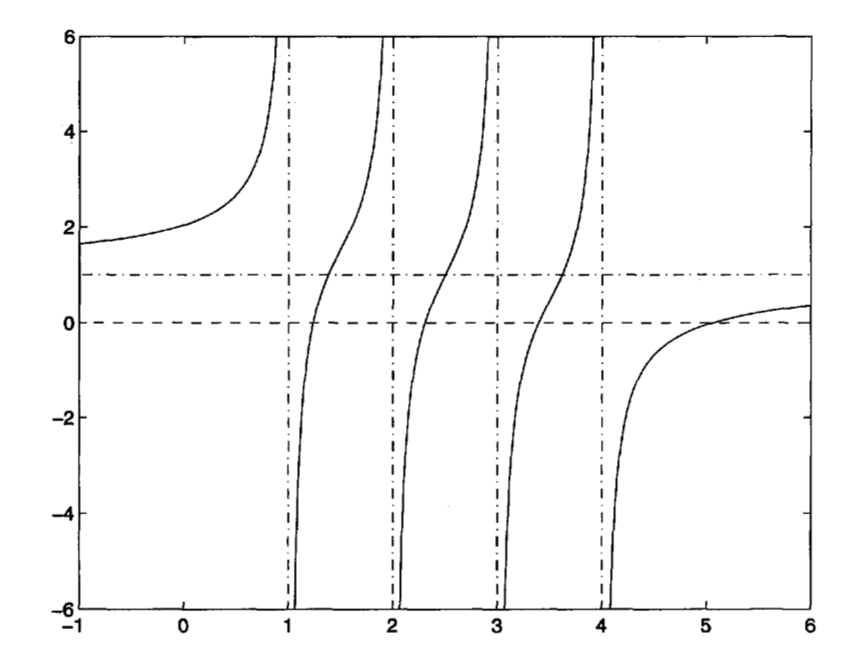
\includegraphics[width = 7cm]{images/lec10-1.png}
    \caption{Graph of $f(\lambda)=1+\frac{.5}{1-\lambda}+\frac{.5}{2-\lambda}+\frac{.5}{3-\lambda}+\frac{.5}{4-\lambda}$}
    \label{fig:10-1}
\end{figure}

Consider figure \ref{fig:10-1}, we see there is one root of $f(\lambda)$ between each pair $[\lambda_i, \lambda_{i+1}]$ of adjacent eigenvalues, 
and in each such interval $f(\lambda)$ is monotonic, so some \textit{Newton}-like method should work well.

\begin{figure}
    \centering
    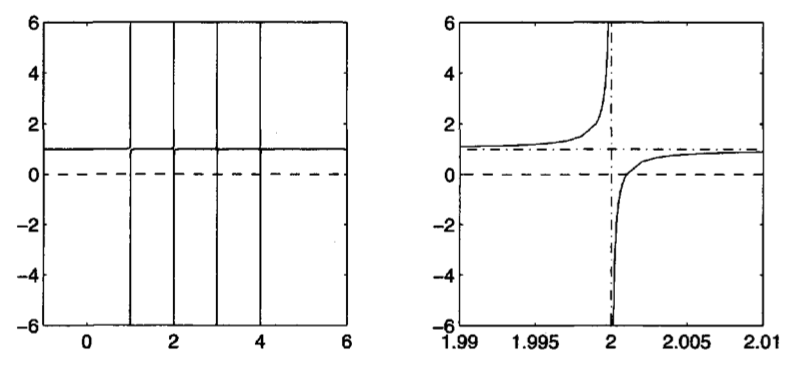
\includegraphics[width = 10cm]{images/lec10-2.png}
    \caption{Graph of $f(\lambda)=1+\frac{10^{-3}}{1-\lambda}+\frac{10^{-3}}{2-\lambda}+\frac{10^{-3}}{3-\lambda}+\frac{10^{-3}}{4-\lambda}$}
    \label{fig:10-2}
\end{figure}

But now consider figure \ref{fig:10-2}. Here $f(\lambda)$ no longer looks so benign, and simple \textit{Newton} would not work,
taking a big step out of the bounding interval. But we can still use \textit{Newton}, but instead of approximating the $f(\lambda)$ by a straight line at each step,
and getting the next guess by finding a zero of that straight line, we approximate $f(\lambda)$ by an simple but non-linear function that better matches the graph, 
with poles at $\lambda_i$ and $\lambda_{i+1}$:
\begin{align*}
    g(\lambda)=c_{1}+ \frac{c_{2}}{\lambda_{i}-\lambda} + \frac{c_{3}}{\lambda_{i+1}-\lambda}
\end{align*}
where $c_1$, $c_2$ and $c_3$ are chosen as in \textit{Newton} to match $f(x)$ and $f^\prime (x)$ at the last approximate 0. 
Solving $g(\lambda)=0$ is then solving a quadratic for $\lambda$.

\begin{figure}[h]
    \centering
    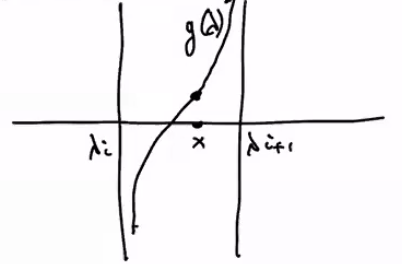
\includegraphics[width = 10cm]{images/lec10-3.png}
    \caption{Graph of $g(\lambda)$}
    \label{fig:10-3}
\end{figure}

\begin{lemma}
    If $\lambda$ is an eigenvector of $\Lambda + \alpha vv^\top$, then $(\Lambda - \lambda I)^{-1}v$ is its eigenvector. Since $\Lambda$ is diagonal, this costs $O(n)$ to compute.
    \begin{proof}
        \begin{align*}
            (\Lambda + \alpha vv^\top)(\Lambda - \lambda I)^{-1}v &= (\Lambda - \lambda I + \lambda I + \alpha vv^\top)(\Lambda - \lambda I)^{-1}v \\
            &= v + \lambda (\Lambda - \lambda I)^{-1} + \underbrace{v\left( \alpha vv^\top (\Lambda - \lambda I)^{-1}v \right)}_{-v \text{ as }f(\lambda)=0} \\
            &= \lambda (\Lambda - \lambda I)^{-1}
        \end{align*}
    \end{proof}
\end{lemma}
Unfortunately this simple formula is not numerically stable; the text describes the clever fix (due to Ming Gu and Stan Eisenstat, 
for which Prof. Gu won the Householder Prize for best thesis in Linear Algebra in 1996).

When two eigenvalues $\lambda_i$ and $lambda_{i+1}$ are (nearly) identical, then we know there is a root between them without doing any work. 
Similarly when $v_i$ is (nearly) zero, we know that $\lambda_i$ is (nearly) an eigenvalue without doing any work. 
In practice a surprising number of eigenvalues can be found quickly ("deflated") this way, which speeds up the algorithm.

Write $\left[Q^{\prime}, \Lambda^{\prime}\right] = \operatorname{Eig\_update}[Q, \Lambda, \alpha,u]$ as the function we just
described that takes the eigendecomposition of $A = Q\Lambda Q^\top$ and updates it,
returning the eigendecomposition of \begin{align*}
    A + \alpha uu^\top = Q^{\prime} \Lambda^\prime Q^{\prime\top}
\end{align*}
We can also use \textit{Eig\_update} as a building block for an entire eigen solver, using Divide-and-Conquer. 
To do so we need to see how to divide a tridiagonal matrix into two smaller ones of half the size,
just using a rank one change $\alpha vv^\top$. We just divide in the middle: If $T=\operatorname{tridiag}\left( a_1, \cdots, a_n, b_1, \cdots, b_{n-1},  \right)$ 
is a symmetric tridiagonal matrix with diagonals $a_i$ and off-diagonals $b_i$, then we can write \begin{align*}
    T = \operatorname{diag}(T_1, T_2) + b_i uu^\top 
\end{align*}
where $T_1$ and $T_2$ are two half-size tridiagonal matrices (if $i$ is $n/2$) and $u$ is a vector with $u_i = u_{i+1}=1$ and the other $u_j=0$.
Using this notation, we can write our overall algorithm as follows:
\begin{algorithmfrm}
    \begin{algorithmic}[1]
        \State $\operatorname{func}[Q, \Lambda]=\text{DC\_eig}(T)$
        \State $n = \operatorname{dimension}(T)$
        \If{$n$ small enough}
            \State use QR iteration
        \Else \State $i = \operatorname{floor}(\frac{n}{2})$
            \State write $T=\operatorname{diag}(T_1, T_2) + b_i uu^\top$ (just notation, no work)
            \State $[Q_1, \Lambda_1]=\text{DC\_eig}(T_1)$
            \State $[Q_2, \Lambda_2]=\text{DC\_eig}(T_2)$ (where $\operatorname{diag}(Q_1, Q_2)$ and $\operatorname{diag}(\Lambda_1, \Lambda_2)$ are the eigendecomposition of $\operatorname{diag}(T_1, T_2)$)
            \State $[Q, \Lambda]=\text{Eig\_update}\left( \operatorname{diag}(Q_1, Q_2), \operatorname{diag}(\Lambda_1, \Lambda_2), b_i, u \right)$
        \EndIf\\
        \Return
    \end{algorithmic}
\end{algorithmfrm}

\subsection{Algorithms for Few Eigenvalues and Eigenvectors Desired}
Now we turn to algorithms that are fastest when only a few eigenvalues and eigenvectors are desired. Afterward we return to briefly describe MRRR, 
the fastest algorithm when all eigenvalues and eigenvectors are desired.

Recall Sylvester's Theorem: Suppose $A$ is symmetric and $X$ nonsingular.
Then $A$ and $X A X^{\top}$ have the same Inertia: \begin{align*}
    (\#\mathrm{evals}<0, \ \#\mathrm{evals}=0, \ \#\mathrm{evals}>0).
\end{align*}
So $A - \sigma I$ and $X(A-\sigma I)X^\top$ have the same Inertia, namely \begin{align*}
    (\#\mathrm{evals} \text{ of }A < \sigma,\ \#\mathrm{evals} \text{ of }A  = \sigma,\ \#\mathrm{evals} \text{ of }A > \sigma)
\end{align*}
So if $X(A-\sigma I)X^\top$ were diagonal, it would be easy to compute Inertia. By doing this for $\sigma_1$ and $\sigma_2$, 
we can count the number of eigenvalues in any interval $[\sigma_1 , \sigma_2]$, and by repeatedly cutting intervals in half, 
we can compute intervals containing the eigenvalues that are as narrow as we like, or that only contain eigenvalues in regions of interest (e.g. the smallest). 

But how do we cheaply choose $X$ to make $X(A-\sigma I)X^\top$ diagonal? By starting with $A = T$ tridiagonal, and doing Gaussian elimination without pivoting: 
\begin{align*}
    T - \sigma I = LDL^\top ,
\end{align*}
so $L^{-1}(T - \sigma I)L^{-\top}$ and $D$ have the same inertia.

However, LU without pivoting seems numerically dangerous. Fortunately, because of the tridiagonal structure, it is not, if done correctly.

\begin{algorithmfrm}[Negcount: count the number $c$ of eigenvalues of $T < s$]
    \begin{algorithmic}
        \LineComment{Only compute diagonal entries $d_i$ of $D$ in $T-sI = LDL^\top$}
        \State Assume $\operatorname{diag}(T) = (a_1, a_2, \cdots, a_n)$
        \State Assume $\operatorname{offdiag}(T) = (b_1, b_2, \cdots, b_{n-1})$
        \State $c = 0$
        \State $b_0 = 0$
        \State $d_0 = 1$
        \For{$i=1:n$}
            \State $d_i = (a_i - s) - b_{i-1}^2/d_{i-1}$\Comment{Obey parentheses!}
            \If{$d_i<0$}
                \State $c=c+1$
            \EndIf
        \EndFor
    \end{algorithmic}
\end{algorithmfrm}

We don't need $l_i$, the $i$-th off diagonal of $L$, because \begin{align*}
    (T-s I)_{i, i+1} = b_i = (LDL^\top)_{i, i+1} = d_i l_i
\end{align*}
so we can replace the usual inner loop of $LDL^\top$ (analogous to LU)
\begin{align*}
    d_i = a_i-s - l_{i-1}^2 d_{i-1}
\end{align*}
by
\begin{align*}
    d_i = a_i-s - \frac{b_{i-1}^2}{d_{i-1}}.
\end{align*}

\begin{theorem}
    Assuming we don't divide by zero, overflow or underflow, the computed $c$ from $\operatorname{Negcount}(T,s)$ is exactly correct for a slightly perturbed $T + E$,
where $E$ is symmetric and tridiagonal,  $E_{ii} = 0$ (the diagonal is not perturbed at all) and \begin{align*}
    |E_{i, i+1}| \leq 2.5 \varepsilon |T_{i, i+1}|
    \end{align*}
    \begin{proof}
        As before, we replace each operation like $a+b$ in the algorithm with $(a+b)(1+\delta)$ where $|\delta| < \varepsilon$. If we obey the parentheses in the algorithm, 
        so $a_i - s$ is subtracted first, then we can divide out by all the $(1+\delta)$ factors multiplying $a_i-s$ to get \begin{align*}
        d_i F_i = a_i-s - \frac{b_{i-1}^2 G_i}{d_{i-1} }
        \end{align*}
        where $F_i$ and $G_i$ are the product of 2 or 3 (1+delta) factors. Now write this as \begin{align*}
            d_i F_i = a_i-s - \frac{b_{i-1}^2 G_i F_{i-1}}{d_{i-1} F_{i-1}}
        \end{align*}
        or \begin{align*}
            d^\prime_{i} = a_i - s - (b^\prime_{i-1})^2 / d^\prime_{i-1},
        \end{align*}
        which is the exact recurrence for $T+E$. Since $d_i$ and $d^\prime_{i} = d_i F_i$ have the same sign, we get the same exact Negcount for either.
    \end{proof}
\end{theorem}

In fact more is true: This works even if some pivot $d_{i-1}$ is exactly zero, and we divide by zero, so the next $d_i$ is infinite, 
because we end up dividing by $d_i$ in the next step, and the "infinity" disappears. But it does mean that to correctly compute Negcount, 
we need to count -0 as negative, and +0 as positive (-0 is a feature of IEEE floating point arithmetic). Furthermore, 
the function $g(\sigma) = \#\mathrm{evals} < \sigma$ is computed monotonically increasing, as long as the arithmetic is correctly rounded 
(otherwise the computed number of eigenvalues in a narrow enough interval might be negative!).

The cost of Negcount is clearly $O(n)$. To find one eigenvalue with Negcount via bisection, Negcount needs to be called at most 64 (in double) or 32 (in single)
times, since each time the interval gets half as big, and essentially determines one more bit in the floating point format. So the cost is still $O(n)$.
So to find $k$ eigenvalues using bisection, the cost is $O(kn)$.

Given an accurate eigenvalue $\lambda_j$ from bisection, we find its eigenvector by inverse iteration:
\begin{algorithmfrm}
    \begin{algorithmic}
        \State Choose $x(0)$, $i=0$
        \While{$x_i$ not converged}
            \State $i = i+1$
            \State Solve $(T - \lambda_j I) y = x(i-1)$ for $y$
            \State $x_i = y / ||y||_2$
        \EndWhile
    \end{algorithmic}
\end{algorithmfrm}
which should converge in a few steps, and so at cost $O(n)$ per eigenvector. This seems like an optimal algorithm for all $n$ eigenvalues and eigenvectors:
at a cost of $O(n)$ per eigenpair, the total cost should be $O(n^2)$. But it has a problem: the computed eigenvectors, 
while they individually very nearly satisfy $Ax = \lambda_j x$ as desired, may not be orthogonal when $\lambda_j$ is very close to another $\lambda_{j+1}$; 
there is nothing in the algorithm to enforce this, and when $\lambda_{j}$ is close to $\lambda_{j+1}$, solving with $T - \lambda_{j}I$ 
is nearly the same as solving with $T - \lambda_{j+1}I$. Imagine the extreme case where $\lambda_j$ and $\lambda_{j+1}$ are so close that they round to the same floating point number!
One could start with a random starting vector $x(0)$ and hope for the best but there is no guarantee of orthogonality.

At first people tried to guarantee orthogonality by taking all the computed eigenvectors belonging to a cluster of nearby eigenvalues and running QR decomposition on them, 
replacing them by the columns of $Q$. This guarantees orthogonality, but has two problems: \begin{enumerate}
    \item If the computed vectors are not linearly independent, the columns of $Q$ may not satisfy $Aq = \lambda q$ very well.
    \item If the size of the cluster of close eigenvalues is $s$, the cost of QR decomposition is $O(s^2 n)$, so if $s$ is large, the cost could go back up to $O(n^3)$.
\end{enumerate}

The MRRR (Multiple Relatively Robust Representations) algorithm was motivated by this problem: computing all the eigenvectors in $O(n^2)$ 
time such that are also guaranteed orthogonal. It is the fastest algorithm available (for large enough problems; it defaults to other algorithms for small problems), 
but is rather complicated to explain. Two lectures explaining it in detail are available from the 2004 Ma221 \href{https://people.eecs.berkeley.edu/~demmel/ma221_Fall04/}{web page}.

The final algorithm of importance is Jacobi's method, whose classical (and so slow) implementation is described in Lecture 5.
Jacobi can be shown to be potentially the most accurate algorithm, with an error determined by a version of Weyl's Theorem for relative error,
and so getting the tiny eigenvalues (and their eigenvectors) much more accurately. It was much slower than the other methods discussed so far, 
until work by Drmac and Veselic showed how it could be made much faster.

All the algorithms discussed so far extend to the SVD, typically by using the relationship between the SVD of $A$ and the eigenvalues and eigenvectors of the
symmetric matrix $\left[\begin{array}{cc}
    0 & A\\
    A^{\top} & O
    \end{array}\right]$. The one exception is MRRR, where some open problems remain, addressed in the 2010 PhD dissertation of Paul Willems,
although there are still examples where Willems’ code loses significant accuracy.

\newpage
\section{Lecture 11: Introduction to Iterative Methods}
\subsection{Introduction to Iterative Methods}
Model Problem: Poisson's Equation \\
\textbf{Goals}: Contrast direct and iterative methods
\begin{itemize}
    \item For $Ax=b$ or least squares: Use iterative methods when direct methods
    are too slow, or use too much memory (from fill-in during factorization) or you don't need as much accuracy.
    \item  $Ax=\lambda x$ or SVD: Use iterative methods for the above reasons, or when only a few eigenvalues/vectors are desired (as well as above reasons).
\end{itemize}
Choosing best iterative method depends on mathematical structure of $A$.
Summary of iterative methods as applied to Model problem, from simple (slow) to sophisticated (fast):
\begin{enumerate}
    \item Simple ones apply to more problems than Model problem
    \item Simple ones are building blocks for more sophisticated ones
\end{enumerate}

Methods covered:\begin{enumerate}
    \item \textit{"Splitting Methods"}: Split $A=M-K$ with $M$ nonsingular. $Ax=b$ becomes $Mx = Kx+b$. Iterate: Solve $Mx_{i+1}=Kx_i +b$ for $x_{i+1}$. Convergence!
    Subtract $Mx = Kx+b$, let $e_i = x_i - x$, then: \begin{align*}
        Me_{i+1} &= Ke_i \\
        e(i+1) &= M^{-1}Ke_i \\
        &= \left( M^{-1}K \right)^{i} e_0
    \end{align*}
    Convergence depends on how fast $\left( M^{-1}K \right)^i \rightarrow 0$. Consider 3 splitting methods: Jacobi,  Gauss-Seidel, and Successive Overrelaxation (SOR).
    \item  \textit{Krylov Subspace Methods (KSMs)}: In the case that you have access to is a subroutine that computes $Ax$ for any $x$, or $A$ is so big that $Ax$ is all you can afford to do.
    With KSMs, given $x_0$:\begin{enumerate}
        \item Compute \begin{align*}
            x_1 = Ax_0, \ x_2 = Ax_1, \ \cdots, \ x_k = Ax_{k-1}
        \end{align*} or a similar set of vectors that span the same subspace
        \item Choose the linear combination $\sum_{i=0}^k a_i x_i$ of these vectors that "best" approximates the answer (for some definition of "best").
        \item If the approximation is not good enough, increase $k$ and repeat.
    \end{enumerate}
    Depending on: \begin{itemize}
        \item How the set of vectors is computed
        \item Properties of $A$ (e.g. symmetry, positive definiteness, \ldots)
        \item The definition of "best approximation"
    \end{itemize}
    One gets a large number of different algorithms, all used in practice:\begin{itemize}
        \item Conjugate Gradients (CG)
        \item Generalized minimum residuals (GMRES)
    \end{itemize}
    and many others. Instead of asking for the "best approximation" to $Ax=b$, one can instead ask for the best approximation to $Ax=\lambda x$.
    \item \textit{Preconditioning}: The speed of the above methods for $Ax=b$ converge is complicated, but in general faster if $\kappa(A)$ smaller.
    Suppose we can find a "preconditioner", i.e. a matrix $M$:\begin{enumerate}
        \item Multiplying by $M$ is cheap
        \item $MA$ is better conditioned than $A$
    \end{enumerate}
    Then one can apply the KSM to solve $MAx=Mb$. Finding good preconditioners can depend in complicated ways on $A$.
    For example, CG depends on $A$ being s.p.d., whereas $MA$ will rarely be symmetric, so need to reorganize CG to use Preconditioning.
    \item \textit{Multigrid}:  This is one of the most effective preconditioners for problems with a suitable mathematical structure, e.g. Poisson's Equation.
    If $A$ arises from solving a physical problem, then straight forward to find an approximation with, say, half as many mesh
    points in each direction, and use the solution of that smaller, and so easier, problem (e.g. $1/4$ the dimension in 2D), as a preconditioner.
    But if the dimension $n$ is very large, so is $n/4$. So we just apply the same idea recursively, using a problem of size $n/16$ to get a starting guess
    for the problem of size n/4, etc. When multigrid works, it can be optimal, solving an $n\times n$ linear system in $O(n)$ flops. 
    But not every problem has the structure that permits this.
    \item \textit{Domain decomposition}: This can be thought of as a way to hybridize the above methods,
    using different methods in different "domains" or submatrices, where A may be easier to work with than as a whole.
\end{enumerate}

Most methods assume the only thing you can afford to do is $y=Ax$. Computing $Ax$ is generally the bottleneck, and usually because of communication:
For example, if $A$ is too large to fit in cache, it needs to be read out of main (slow) memory every iteration,
with only one multiplication and addition per entry. So recent work has addressed communication-avoiding KSMs, 
where methods like CG are redesigned to take $s>1$ steps for each access of $A$, instead of 1 step.

\subsection{Model Problem: Poisson's Equation}
1D with Dirichlet boundary conditions:\begin{align*}
    -\frac{\partial^{2}}{\partial x^{2}} v(x)=f(x)
\end{align*}
on $x \in [0,1]$, $v(0)=v(1)=0$. Discretizing to get:\begin{align*}
    T_N \left[\begin{array}{c}v_{1} \\ \vdots \\ v_{N}\end{array}\right] &= T_N v \\
    &= h^2 \left[\begin{array}{c}f_{1} \\ \vdots \\ f_{N}\end{array}\right] \\
    &= h^2 f \\
    T_N &= \left[\begin{array}{cccc}2 & -1 & & \mathbf{O} \\ -1 & \ddots & \ddots & \\ & \ddots & \ddots & -1 \\ \mathbf{O} & & -1 & 2\end{array}\right]
\end{align*}

\begin{lemma}
    $T_{N} z_{j}=\lambda_{j} z_{j}$ where \begin{align*}
        \lambda_{j}&=2\left(1-\cos \frac{\pi j}{N+i}\right) \\
        z_{j}(k)&=\sqrt{\frac{2}{N+1}} \sin \left( \frac{j k \pi}{N+c} \right)
    \end{align*}
\end{lemma}
\begin{corollary}
    The matrix $Z$ where \begin{align*}
        z_{j}(k)&=\sqrt{\frac{2}{N+1}} \sin \left( \frac{j k \pi}{N+c} \right)
    \end{align*}
    is orthogonal (related to Fast Fourier Transform).
\end{corollary}
Eigenvalues range from the smallest one $\lambda_j \sim \left( \frac{\pi j}{N+1} \right)^2$ up to $\lambda_N \sim 4$, which tells the condition number of $T_N$:\begin{align*}
    \frac{\lambda_N}{\lambda_1} &\sim \left( \frac{2\left( N+1 \right)^2}{\pi} \right)^2 \\
    &=\left( \frac{2}{\pi} \right) h^{-2}
\end{align*}

2D with Dirichlet boundary conditions:\begin{align*}
    \frac{-\partial^{2}}{\partial x^{2}} v(x, y)-\frac{\partial^{2}}{\partial y^{2}} v(x, y) = f(x, y)
\end{align*}
on square $[0,1]^2$ with $v(x,y)=0$ on boundary. Discretize as before, write $v_{i,j}=v(i \cdot h, j\cdot h)$, then \begin{align*}
    4v_{ij} - v_{i-1,j} - v_{i+1,j} - v_{i,j-1} - v_{i,j+1} = h^2 f_{ij}
\end{align*}
Letting $V$ be the $N\times N$ matrix of $v_{ij}$, we can also write \begin{align*}
    & 2v_{ij} - v_{i-1,j} - v_{i+1,j} = (T_N V)_{ij} \\
    & 2v_{ij} - v_{i,j-1} - v_{i,j+1} = (V T_N )_{ij}
\end{align*}
Then the above equation becomes $(T_N V + V T_N )_{ij}$ or \begin{align*}
    T_N V + V T_N=h^2 F
\end{align*}
a system of $N^2$ linear equations for the $N^2$ entries of $V$, though not in the usual "$Ax=b$" form.
We can ask about the corresponding eigenvalues and eigenvectors in the analogous form:\begin{align*}
    T_N V + V T_N=\lambda V
\end{align*}
Suppose $T_N z_i = \lambda_i z_i$ and $T_N z_j = \lambda_j z_j$ are any two eigen pairs of $T_N$. Letting $V = z_i  z_j^\top$, we get \begin{align*}
    T_N V + V T_N &= (T_N z_i) z_j^\top + z_i (z_j^\top T_N) \\
    &= (\lambda_i z_i) z_j^\top + z_i (\lambda_j z_j^\top) \\
    &= \left( \lambda_i + \lambda_j \right) z_i z_j^\top \\
    &= \left( \lambda_i + \lambda_j \right) V
\end{align*}
Hence, $V=z_i z_j^\top$ is an eigenvector with eigenvalue $\lambda_i + \lambda_j$. Since there are $N^2$ pairs of $(i,j)$, we are expecting $N^2$ pairs of eigenvalues and eigenvectors.
We want to write $V$ as a single vector in a way that easily extends to higher dimensional Poisson equations. In the $3\times 3$ case, write $V$ columnwise from left to right as:\begin{align*}
    v = [ v_{11}; v_{21}; v_{31}; v_{12}; v_{22}; v_{32}; v_{13}; v_{23}; v_{33} ]
\end{align*}
and $T_{N \times N}$ has the following patterns rowwise:\begin{itemize}
    \item 4 on the diagonal multiplies $v_{ij}$
    \item -1s next to the diagonal multiply $v_{i-1,j}$ and $v_{i+1,j}$
    \item -1s $N$ away from the diagonal multiply $v_{i,j-1}$ and $v_{i,j+1}$
\end{itemize}
Note that some rows have fewer than $4 -1s$, when these are on the boundary of the square. One may confirm that \begin{align*}
    T_{N \times N} V = h^2 f
\end{align*}
Another way to write $T_{N \times N}$ is \begin{align*}
    \left[\begin{array}{ccc}T_{N}+2 I_{N} & -I_{N} & \\ -I_{N} & T_{N}+2 I_{N} & -I_{N} \\ & \ddots & \\ & -I_{N} & T_{N}+2 I_{N}\end{array}\right]
\end{align*}
a pattern we will generalize to arbitrary dimensions, using Kronecker products.

\subsection{Poisson's Equation in d Dimensions}
\begin{definition}
    Let $X$ be an $m \times n$ matrix. Then $\operatorname{vec}(X)$ is $mn \times 1$ gotten by stacking the columns of $X$ on top of one another, from left to right.
\end{definition}

\begin{definition}
    Let $A$, $B$ be $m \times n$, $p \times q$ matrices respectively. Then $A \otimes B$ is the $mp \times nq$ matrix \begin{align*}
        \left[\begin{array}{ccc}A_{11} {B} & \cdots & A_{1 n} {B} \\ \vdots & \ddots & \vdots \\ A_{m 1} {B} & \cdots & A_{m n} {B}\end{array}\right]
    \end{align*}
    is the Kronecker product of $A$ and $B$.
\end{definition}

\begin{lemma}
    Let $A$, $B$, $X$ be $m \times m$, $n \times n$, $m \times n$ matrices respectively. Then, \begin{enumerate}
        \item $\operatorname{vec}(AX) = \left( I_n \otimes A \right) \operatorname{vec}(X)$
        \item $\operatorname{vec}(XB) = \left( B^\top \otimes I_m \right) \operatorname{vec}(X)$
        \item  The 2D Poisson's equation $T_N V + V T_N=h^2 F$ can be written as follows: \begin{align*}
            \left( I_N \otimes T_N + T_N \otimes I_N \right) \operatorname{vec}(V) = h^2 \operatorname{vec}(F)
        \end{align*}
    \end{enumerate}
    \begin{proof}
        \begin{enumerate}
            \item Since $I_n \otimes A=\operatorname{diag}\left( \underbrace{A, A, \cdots, A}_n \right)$, \begin{align*}
                \left( I_n \otimes A \right) \operatorname{vec}(X) &= \left[\begin{array}{llll}A & & & \\ & A &  & \\ & & \ddots & \\ & & & A\end{array}\right]
                \left[\begin{array}{c} X_{i, 1} \\ X_{i, 2} \\ \vdots \\ {X}_{i, n}\end{array}\right] \\
                &= \left[\begin{array}{c}A X_{i, 1} \\ AX_{i, 2} \\ \vdots \\ A{X}_{i, n}\end{array}\right] \\
                &= \operatorname{vec}(AX)
            \end{align*}
            \item Similar.
            \item  Apply part 1 to $T_N V$ and part 2 to $V T_N$, noting that $T_N$ is symmetric. Then,\begin{align*}
                I_N \otimes T_N + T_N \otimes I_N &= \left[\begin{array}{llll}T_N & & & \\ & T_N &  & \\ & & \ddots & \\ & & & T_N\end{array}\right] + 
                \left[\begin{array}{ccc}2 I_{N} & -I_{N} & \\ -I_{N} & 2 I_{N} & -I_{N} \\ & \ddots & \\ & -I_{N} & 2 I_{N}\end{array}\right]
            \end{align*}
        \end{enumerate}
    \end{proof}
\end{lemma}

\begin{lemma}
    \begin{enumerate}
        \item Assume that $AC$ and $BD$ are well defined. Then,\begin{align*}
            (A \otimes B)(C \otimes D) = (AC) \otimes (BD)
        \end{align*}
        \item If $A$ and $B$ are invertible, then, \begin{align*}
            (A \otimes B)^{-1} = (A^{-1}) \otimes (B^{-1})
        \end{align*}
        \item \begin{align*}
            (A \otimes B)^{\top} = (A^{\top}) \otimes (B^{\top})
        \end{align*}
    \end{enumerate}
\end{lemma}

\begin{proposition}
    $T=Z \Lambda Z^{\top}$ be eigendecomposition of $N \times N$ symmetric $T$. Then the eigendecomposition of \begin{align*}
        I \otimes T+T \otimes I &= (Z \otimes Z)(I_N \otimes \Lambda + \Lambda \otimes I_N) (Z^\top \otimes Z^\top)
    \end{align*}
    where the first part on the right side of the equation is a diagonal matrix with entry \begin{align*}
        (I_N \otimes \Lambda + \Lambda \otimes I_N)_{(i-1)N + j} = \lambda_i + \lambda_j
    \end{align*}
    $Z \otimes Z$ is orthogonal with $\left( (i-1)N + j \right)$th column \begin{align*}
        z_i \otimes z_j
    \end{align*}
    \begin{proof}
        Multiply out the factorization using the last lemma to get \begin{align*}
            (ZI_N \otimes Z\Lambda + Z\Lambda \otimes Z I_N)(Z^\top \otimes Z^\top) &= ZI_N Z^\top \otimes Z\Lambda Z^\top + Z\Lambda Z^\top \otimes Z I_N Z^\top \\
            &= I_N \otimes T+T \otimes I_N
        \end{align*}
    \end{proof}
\end{proposition}

Similarly, Poisson's equation in 3D leads to the matrix \begin{align*}
    T_{N\times N\times N} &= \left(T_{N} \otimes I_{N} \otimes {I}_{N}\right) + \left(I_{N} \otimes T_{N} \otimes {I}_{N}\right) + \left(I_{N} \otimes I_{N} \otimes T_{N}\right)
\end{align*}
with eigenvalue matrix \begin{align*}
    \left(\Lambda_{N} \otimes I_{N} \otimes {I}_{N}\right) + \left(I_{N} \otimes \Lambda_{N} \otimes {I}_{N}\right) + \left(I_{N} \otimes I_{N} \otimes \Lambda_{N}\right)
\end{align*}
i.e. $N^3$ eigenvalues $\lambda_i + \lambda_j + \lambda_k$ for all triples $(i,j,k)$, and corresponding eigenvector matrix $Z \otimes Z \otimes Z$.
Poisson's equation equation in $d$ dimensions is similarly represented.

\subsection{Solving Poisson's Equation with Fast Fourier Transform}
We now know enough to describe how to solve Poisson's equation with the FFT. This is a direct method, not iterative, but we want to compare it to the other methods.
We describe it first for 2D Poisson, and then how to extend to higher dimensions. Start with 2D Poisson \begin{align*}
    T_N V + V T_N = F
\end{align*}
which is a special case of the Sylvester equation described in Question 4.6: We substitute the eigendecomposition \begin{align*}
    T=Z \Lambda Z^{\top}
\end{align*} yielding \begin{align*}
    Z\Lambda Z^{\top} V+V Z{\Lambda} Z^{\top}=F
\end{align*}
Pre-multiply by $Z^\top$ and post-multiply by $Z$, yielding \begin{align*}
    \Lambda Z^{\top} VZ + Z^{\top} VZ \Lambda = Z^{\top} FZ
\end{align*}
Rename $V^\prime = Z^\top VZ$ and $F^\prime = Z^\top FZ$, yielding \begin{align*}
    \Lambda V^\prime + V^\prime \Lambda = F^\prime
\end{align*}
Since Lambda is diagonal, this is a diagonal system of equations, with \begin{align*}
    \left( \Lambda V^\prime + V^\prime \Lambda \right)_{ij} = \lambda_i V^\prime_{ij} + \lambda_j V^\prime_{ij} = F^\prime_{ij}
\end{align*} or \begin{align*}
    V^\prime_{ij} = \frac{F^\prime_{ij}}{\lambda_i + \lambda_j}
\end{align*}
This yields the overall algorithm:
\begin{algorithmfrm}
    \begin{enumerate}
        \item Compute $F^\prime = Z^\top FZ$
        \item Compute $V^\prime_{ij} = \frac{F^\prime_{ij}}{\lambda_i + \lambda_j}$ for all $i$, $j$
        \item Compute $V=ZV^\prime Z^\top$
    \end{enumerate}
\end{algorithmfrm}
The main costs are the matrix multiplications by $Z$ and $Z^\top$ in (1) and (3), which would cost $O(N^3)$ if done straightforwardly.
But they can be done in $O(N^2 \log N)$ operations (recall $N^2$ is the number of unknowns) by noting that $Z$ is closely related to the Fast Fourier Transform matrix: \begin{align*}
    \operatorname{FFT}_{ij} &= \exp \left( 2\pi \sqrt{-1} ij / N \right) \\
    &= \cos \frac{\pi ij}{N} + \underbrace{\sqrt{-1} \sin \frac{\pi ij}{N}}_Z
\end{align*}
for which there are $O(N\log N)$ methods for multiplication by a vector.\\
The same idea extends to high dimensions by using Kronecker product notation: \begin{align*}
    I_{N} \otimes T_{N} + T_{N} \otimes I_{N} &= (Z \otimes Z)\left(I_{N} \otimes \Lambda+\Lambda \otimes I_{N}\right)(Z^{\top} \otimes Z^{\top})
\end{align*}
So, \begin{align*}
    (I_{N} \otimes T_{N} + T_{N} \otimes I_{N})^{-1} &= (Z^{\top} \otimes Z^{\top})^{-1} (I_{N} \otimes \Lambda+\Lambda \otimes I_{N})^{-1} (Z \otimes Z)^{-1} \\
    &= (Z \otimes Z)\left( D \right)^{-1}(Z^{\top} \otimes Z^{\top})
\end{align*}
where $D$ is a diagonal matrix with diagonal entries $\sum \lambda_i + \lambda_j + \lambda_k$.

\subsection{Summary of performance of methods for Poisson's Equation}
We will count \#Flops, Memory needed, \#Parallel Steps, and \#Procs.
"Parallel Steps" is the fewest possible, on a machine with as many processors as needed (given by \#Procs), 
and so it refers only to the available parallelism, not how you would actually implement it on a real machine with a smaller number of processors.

The algorithms are sorted in two related orders: from slowest to fastest for the Poisson's Equation, and (roughly) from most general (fewest assumptions about the matrix) to least general.

Here are some explanations and abbreviations. 
Explicit inverse assumes we have pre-computed the exact inverse of the matrix $A^{-1}$ (do not count cost of it) and only need to multiply by it.
\begin{itemize}
    \item SOR: Successive overrelaxation
    \item SSOR/Chebyshev: Symmetric SOR with Chebyshev Acceleration
    \item FFT: Fast Fourier Transform
    \item BCR: Block Cyclic Reduction
    \item Lower Bound: The lower bound that assumes one flop per component of the output vector
    \item SpMV: Sparse-matrix times dense-vector multiplication, where the cost equals to the number of nonzeros.
\end{itemize}
For 2D Poisson on an $n \times n$ mesh, \begin{align*}
    N = n^2 = \# \text{unknowns}
\end{align*}
For 3D Poisson on an $n \times n \times n$ mesh, \begin{align*}
    N = n^3 = \# \text{unknowns}
\end{align*}
If table entry for 2D and 3D differ, 3D shown in parentheses. All the table entries are meant in a Big-Oh sense.

\begin{savenotes}
    \begin{table}[H]
        \centering
        \begin{tabular}{|l|l|l|l|l|l|}
            \hline
            Method & Direct or Iterative & \#Flops & Memory & \#Parallel Steps & \#Procs \\ \hline
            Dense Cholesky\footnote{Works on any spd matrix} & D & $N^3$ & $N^2$ & $N$ & $N^2$ \\ \hline
            Explicit Inverse & D & $N^2$ & $N^2$ & $\log N$ & $N^2$ \\ \hline
            Band Cholesky\footnote{Works on any banded spd matrix with cost $O(N \text{bw}^2)$. 2D: $\text{bw}=n=N^{1/2}$, 3D: $\text{bw}=n^2=N^{2/3}$} & D & \makecell[l]{$N^2$ \\ $(N^{7/3})$} & \makecell[l]{$N^{3/2}$ \\ $(N^{5/3})$} & N & \makecell[l]{$N$ \\ $(N^{4/3})$} \\ \hline
            Jacobi\footnote{$O(\#\text{Flops(SpMV)} \cdot \#\text{iterations})$} & I & \makecell[l]{$N^2$ \\ ($N^{5/3}$)} & $N$ & \makecell[l]{$N$ \\ ($N^{2/3}$)} & $N$ \\ \hline
            Gauss-Seidel\footnote{Cost analogous to Jacobi (constants differ). Works on any diagonally dominant or spd matrix} & I & \makecell[l]{$N^2$ \\ ($N^{5/3}$)} & $N$ & \makecell[l]{$N$ \\ ($N^{2/3}$)} & $N$ \\ \hline
            Sparse Cholesky\footnote{Assumes we are using the best ordering known (nested dissection)
            Works on any spd matrix; complexity arises from cost of dense Cholesky on trailing $n \times n$ submatrix (in 2D) or $n^2\times n^2$ submatrix (in 3D)} & D & \makecell[l]{$N^{3/2}$ \\ ($N^{2}$)} & \makecell[l]{$N \log N$ \\ ($N^{4/3}$)} & \makecell[l]{$N^{1/2}$ \\ ($N^{2/3}$)} & \makecell[l]{$N$ \\ ($N^{4/3}$)} \\ \hline
            Conjugate Gradients\footnote{Works on any spd matrix. $\#\text{Flops}=O(\#\text{Flops}(\text{SpMV}) \cdot \#\text{iterations})$, where $\#\text{iterations}=O(\sqrt{\operatorname{cond}(A)})$} & I & \makecell[l]{$N^{3/2}$ \\ ($N^{4/3}$)} & $N$ & \makecell[l]{$N^{1/2}\log N$ \\ ($N^{1/3}\log N$)} & $N$ \\ \hline
            SOR\footnote{Cost analysis analogous to Conjugate Gradients. Works on any spd matrix, convergence rate depends on cond} & I & \makecell[l]{$N^{3/2}$ \\ ($N^{4/3}$)} & $N$ & \makecell[l]{$N^{1/2}$ \\ ($N^{4/3}$)} & $N$ \\ \hline
            SSOR/Chebyshev\footnote{Works on any spd matrix, but need to know range of eigenvalues. $\#\text{Flops}=O(\#\text{Flops}(\text{SpMV}) \cdot \#\text{iterations})$, where $\#\text{Flops}(\text{SpMV})=O(\#\text{nonzeros in }A)$ and $\#\text{iterations}=\frac{1}{4}\operatorname{cond}(A)$} & I & \makecell[l]{$N^{5/4}$ \\ ($N^{7/6}$)} & $N$ & \makecell[l]{$N^{1/4}$ \\ ($N^{1/6}$)} & $N$ \\ \hline
            FFT\footnote{Works on Poisson} & D & $N \log N$ & $N$ & $\log N$ & $N$ \\ \hline
            BCR\footnote{Works on problems slightly more general than model problem} & D & $N \log N$ & $N$ & ? & ? \\ \hline
            Multigrid\footnote{Many variants,  which work quite generally on problems arising from elliptic PDE and FEM models} & I & $N$ & $N$ & $\log^2 N$ & $N$ \\ \hline
            Lower Bound &  & $N$ & $N$ & $\log N$ &  \\ \hline
        \end{tabular}
    \end{table}
\end{savenotes}

\newpage
\section{Lecture 12: Splitting Methods}
\subsection{Splitting Methods}
\textbf{Goal}: given an initial guess $x_0$ for a solution of $Ax=b$, cheaply compute a sequence $x_i$ converging to $A^(-1)b$.

\begin{definition}
    A splitting of $A$ is a decomposition $A = M - K$ with $M$ nonsingular.
\end{definition}

This yields the following iterative method: Write $A x = M x - K x = b$.
so $M x=K x+b$. Then compute $x_{i+1}$ from $x_1$ by solving \begin{align*}
    M x_{i+1}=Kx_{i}+b
\end{align*}
or \begin{align*}
    x_{i+1} &=M^{-1}Kx_{i}+M^{-1}b \\
    &= Rx_i + c \quad (*)
\end{align*}
For this to work well, we need two conditions:\begin{enumerate}
    \item It should converge
    \item Multiplying by $R$ (i.e. solving $M x_{i+1}=Kx_{i}+b$ for $x_{i+1}$) and computing $c = M^{-1}b$ should be much cheaper than solving with $A$ itself
\end{enumerate}

\begin{lemma}
    Let $\norm{\cdot}$ be any operator norm. Then if $\norm{R}<1$, $(*)$ converges to $A^{-1}b$ for any $x_0$.
    \begin{proof}
        Subtract $x = Rx + c$ from $x_{i+1} = Rx_i+c$ to get \begin{align*}
            x_{i+1} - x = R(x_i-x)+c
        \end{align*}
        or \begin{align*}
            \norm{x_{i+1} - x} \leq \norm{R} \norm{x_{i+1} - x} \leq \cdots \leq \norm{R}^{i+1} \norm{x_{0} - x}
        \end{align*}
        which converges to zero for any $x_0$ if $\norm{R}<1$.
    \end{proof}
\end{lemma}

\begin{definition}
    The spectral radius of $R$ is $\operatorname{rho}(R) = \max |\lambda|$, the largest absolute value of any eigenvalue of $R$.
\end{definition}

\begin{lemma}
    For all operator norms, $\rho(R) \leq \norm{R}$. For all $R$ and all $\varepsilon>0$,
    there exists an operator norm $\norm{\cdot}^*$ such that \begin{align*}
        \norm{R}^* \leq \rho(R) + \varepsilon
    \end{align*}
    \begin{proof}
        To show $\rho(R) \leq \norm{R}$, note that $\norm{R} = \max_{x \neq 0}\frac{\norm{Rx}}{\norm{x}}$,
        By picking $x$ to be an eigenvector, we see that $\norm{R} \geq |\lambda|$ for any eigenvalue $\lambda$ of $R$. 
        To construct $\norm{\cdot}^*$, use the Jordan form of $R$:\begin{align*}
            S^{-1} R S=J
        \end{align*}
        i.e. $J$ is block diagonal with Jordan blocks. Let $D = \operatorname{diag}(1,\varepsilon,\varepsilon^2,\cdots,\varepsilon^{n-1})$. 
        Then $J_\varepsilon = D^{-1}JD$ leaves the diagonal (eigenvalues) unchanged, and multiplies each superdiagonal entry of $J$ by $\varepsilon$, so $J$ has eigenvalues on the diagonal,
        and $\varepsilon$ above the diagonal in any Jordan block. We now define a new vector norm by $\norm{x}^* = \norm{(SD)^{-1}x}_\infty$.
        Then, \begin{align*}
            \norm{R}^* &= \max_{x \neq 0} \frac{\left\|R{x}\right\|^{*}}{\|x\|^{*}} \\
            &= \max_{x \neq 0} \frac{\left\|(SD)^{-1}R{x}\right\|_{\infty}}{\|\underbrace{(SD)^{-1}x}_{y}\|_{\infty}} \\
            &= \max_{y \neq 0} \frac{\left\|(SD)^{-1}R(SD)y\right\|_{\infty}}{\|y\|_{\infty}} \\
            &= \max_{y \neq 0} \frac{\left\|J_\varepsilon y\right\|_{\infty}}{\|y\|_{\infty}} \\
            &\leq \max |\lambda| + \varepsilon \\
            &= \rho(R) + \varepsilon
        \end{align*}
    \end{proof}
\end{lemma}

\begin{theorem}
    The iteration $x_{i+1} = Rx_i + c$ converges to $A^{-1}b$ for all starting vectors $x_0$ if and only if $\rho(R)<1$.
    \begin{proof}
        If $\rho(R) \geq 1$, chose $x_0$ so that $x_0-x$ is an eigenvector of $R$ for its largest eigenvalue $\lambda$. 
        Then $x_i-x = R^i(x_0-x) = \lambda^i (x_0-x)$ does not converge to zero since $|\lambda| \geq 1$.
        If $\rho(R) < 1$, use the last lemma to conclude that there is an operator norm $\norm{R}^*$ and an $\varepsilon$ such that \begin{align*}
            \norm{R}^* \leq \rho(R)+\varepsilon < 1,
        \end{align*}so that $x_i-x = R^i (x_0-x)$ converges to zero for all $x_0$.
    \end{proof}
\end{theorem}

Obviously, the smaller is $\rho(R)$, the faster is convergence. Our goals is to pick the splitting $A = M-K$ so that multiplying by $R = M^{-1}K$ is easy, 
and $\rho(R)$ is small. Choosing $M = I$ and $K = I-A$ makes multiplying by $R$ easy, but will not generally make $rho(R)$ small. 
Choosing $K = 0$ and so $R = 0$ makes convergence immediate, but requires having the solution $c = A^{-1}b$.

\subsection{Describe Jacobi \& Gauss-Seidel \& SOR}
All share the notation $A = D - L^\prime - U^\prime = D(I - L - U)$, where $D$ is the diagonal of $A$, $L^\prime$ is the negative of the strictly lower triangular part, 
and $U^\prime$ is the negative of the strictly upper triangular part of $A$.

\subsubsection{Jacobi}
\begin{itemize}
    \item In words: For $j=1$ to $n$, pick $x_{i+1}(j)$ to exactly satisfy equation $j$
    \item As a loop:
    \begin{algorithmfrm}
        \begin{algorithmic}[1]
            \For{$j=1:n$}
            \State $x_{i+1}(j)=\left( b_j - \sum_{k \neq j} A_{jk}x_i(k) / A_{jj} \right)$
            \EndFor
        \end{algorithmic}
    \end{algorithmfrm}
    \item As a splitting: $A = D - (L^\prime+U^\prime) = M - K$, so 
    \begin{align*}
        R_J = M^{-1}K = D^{-1}(L^\prime+U^\prime) = L+U    
    \end{align*}
    \item For the 2D Poisson equation $T_N V+V T_N = h^2 F$, to get from $V_i$ to $V_{i+1}$:
    \begin{algorithmfrm}
        \begin{algorithmic}[1]
            \For{$j=1:n$}
            \For{$k=1:n$}
            \State $V_{i+1}(j,k) = (V_i(j-1,k) + V_i(j+1,k) + V_i(j,k-1) + V_i(j,k+1) + h^2 F(j,k))/4$ \Comment{"Average" of 4 nearest neighbors and right-hand-sid}
            \EndFor
            \EndFor
        \end{algorithmic}
    \end{algorithmfrm}
\end{itemize}

\subsubsection{Gauss-Seidel}
\begin{itemize}
    \item In words: Improve on Jacobi by using most recently updated values of solution
    \item As a loop:
    \begin{algorithmfrm}
        \begin{algorithmic}[1]
            \For{$j=1:n$}
            \State $x_{i+1}(j)=\left( b_j - \sum_{k < j} A_{jk}x_{i+1}(k) \right) - \sum_{k > j} A_{jk}x_i(k) / A_{jj}$ \Comment{Updated $x$ components minus older $x$ components}
            \EndFor
        \end{algorithmic}
    \end{algorithmfrm}
    \item As a splitting: $A = (D - L^\prime) - U^\prime = M - K$, so 
    \begin{align*}
        R_{GS} &= (D-L^\prime)^{-1}U^\prime \\
        &= (D(I-D^{-1}L^\prime))^{-1}U^\prime \\
        &= (I - L)^{-1} U
    \end{align*}
    Note that the order in which we update entries matters in GS (unlike Jacobi).
    \item For the 2D Poisson there are two orders to consider: natural order (rowwise or columnwise update of $V(i,j)$)
    Red-Black (RB) ordering: color the entries in the 2D mesh like a checkerboard, and number the Reds before all the Blacks. 
    Note that each Red node only has Black neighbors, and vice-versa. Thus when updating Red nodes, 
    we can update them in any order, since all the Black neighbors have old data. Then when we update the Black nodes, 
    we can update them in any order, because all the Red neighbors have new data.
    \begin{algorithmfrm}
        \begin{algorithmic}[1]
            \For{all $(j,k)$ nodes that are Red}\Comment{$j+k$ even}
            \State $V_{i+1}(j,k) = (V_i(j-1,k) + V_i(j+1,k) + V_i(j,k-1) + V_i(j,k+1) + h^2 F(j,k))/4$ \Comment{Only use old data}
            \EndFor
            \For{all $(j,k)$ nodes that are Black}\Comment{$j+k$ odd}
            \State $V_{i+1}(j,k) = (V_{i+1}(j-1,k) + V_{i+1}(j+1,k) + V_{i+1}(j,k-1) + V_{i+1}(j,k+1) + h^2 F(j,k))/4$ \Comment{Only use new data}
            \EndFor
        \end{algorithmic}
    \end{algorithmfrm}
\end{itemize}

\subsubsection{Successive Overrelaxation (SOR)}
\begin{itemize}
    \item In words: This depends on a parameter $w$: We let the result of SOR be a weighted combination of the old ($x_i$) and new ($x_{i+1}$) solutions that GS would have computed: \begin{align*}
        x^{\operatorname{SOR}(w)}_{i+1}(j) = (1-w) x_i(j) + wx^{\operatorname{GS}}_{i+1}(j)    
    \end{align*}
    When $w=1$, $\operatorname{SOR}(1)$ is just GS. When $w<1$ we would call this underrelaxation, and when $w>1$, we call it overrelaxation. 
    We prefer to "overrelax" with the intuition that if moving in the direction from $x_i$ to $x_{i+1}$ was a good idea, moving even farther in the same direction is better.
    Later we will show how to pick w optimally for the model problem.
    \item As a loop:
    \begin{algorithmfrm}
        \begin{algorithmic}[1]
            \For{$j=1:n$}
            \State $x_{i+1}(j)=(1-w)x_i(j) + w \left( b_j - \sum_{k < j} A_{jk}x_{i+1}(k) \right) - \sum_{k > j} A_{jk}x_i(k) / A_{jj}$ \Comment{Updated $x$ components minus older $x$ components}
            \EndFor
        \end{algorithmic}
    \end{algorithmfrm}
    \item As a splitting: Multiply through by $D$ to get \begin{align*}
        (D-wL^\prime) x_{i+1} = \left( (1-w)D + wU^\prime \right)x_i + wb
    \end{align*}
    and then divide by $w$ to get the splitting \begin{align*}
        A &= (D/w - L^\prime) - (D/w- D + U^\prime) \\
        &= M - K
    \end{align*}
    or
    \begin{align*}
        R_{\operatorname{SOR}(w)} &= (D/w-L^\prime)^{-1} (D/w - D + U^\prime) \\
        &= (I-w L)^{-1} \left( (1-w)I +wU \right)
    \end{align*}
    \item For the 2D Poisson with Red-Black Ordering:
    \begin{algorithmfrm}
        \begin{algorithmic}[1]
            \For{all $(j,k)$ nodes that are Red}\Comment{$j+k$ even}
            \State $V_{i+1}(j,k) = (1-w)V_i(j,k) + w(V_i(j-1,k) + V_i(j+1,k) + V_i(j,k-1) + V_i(j,k+1) + h^2 F(j,k))/4$ \Comment{Only use old data}
            \EndFor
            \For{all $(j,k)$ nodes that are Black}\Comment{$j+k$ odd}
            \State $V_{i+1}(j,k) = (1-w)V_i(j,k) + w(V_{i+1}(j-1,k) + V_{i+1}(j+1,k) + V_{i+1}(j,k-1) + V_{i+1}(j,k+1) + h^2 F(j,k))/4$ \Comment{Only use new data}
            \EndFor
        \end{algorithmic}
    \end{algorithmfrm}
\end{itemize}

\subsection{Convergence of Splitting Methods}
Now we analyze the convergence of these basic methods, in general and for the Model Problem (2D Poisson) in particular.

\begin{itemize}
    \item Jacobi: For the Model problem, it is easy to analyze, since in the splitting \begin{align*}
        T_{n\times n} = M - K = 4I - (4I - T_{n\times n}),    
    \end{align*}
    so \begin{align*}
        R = M^(-1)K = I - T_{n\times n} / 4,
    \end{align*} 
    so the eigenvalues of R are $1 - (\lambda_i+\lambda_j)/4$. For all pairs of eigenvalues, \begin{align*}
        \lambda_i = 2(1-\cos(\frac{i\pi}{n+1})),
    \end{align*}
    and so the spectral radius $\rho(R)$ of $R$ is \begin{align*}
        1 - \frac{\lambda_{\text{min}}}{2} = 1 - (1 - \cos\frac{\pi}{n+1}) \\
        &= \cos\frac{\pi}{n+1} \\
        &~ 1 - \frac{\pi^2}{2(n+1)^2}
    \end{align*}
    which gets closer to 1 as $n$ grows, i.e. Jacobi converges more slowly. Since the error after $m$ steps is multiplied by $\rho(R)^m$,
    we estimate the speed of convergence by computing how many steps $m$ are needed to reduce the error by a constant factor. 
    Setting $\rho(R) = 1 - x$, $x \ll 1$,
    \begin{align*}
        \rho(R) &= (1-x)^m \\
        &= (1-x)^{\frac{1}{x}mx} \\
        &\approxeq (e^{-1})^{mx} \\
        &= e^{-mx} 
    \end{align*}
    $e^{-m x} \approx e^{-1}$ implies that $m = \frac{1}{x}$. For Jacobi, \begin{align*}
        \frac{1}{x} &= \frac{2(n+1)^{2}}{\pi^{2}} \\
        &= O(n^2) \\
        &= O(N)
    \end{align*}
    where $N=n^2$ is the number of unknowns. Note that $\operatorname{cond}(T_{n\times n}) ~ \frac{4N}{\pi^2}$ is also $O(N)$.
    So the number of iterations grows proportionally to the dimension $N$, and to the condition number.
    So to reduce the error by any constant factor costs $O(N)$ iterations times $O(N)$ flops\_per\_iteration, or $O(N^2)$ overall, 
    explaining the entry in the table above. This is typical for many iterative methods: 
    the number of iterations grows with the condition number (multigrid is an important exception!).
    \item Gauss Seidel: Assuming variables updated in right order for 2D Poisson, 
    we get $\rho(R_{\operatorname{GS}}) = \rho(R_J)^2$, i.e. one step of Gauss-Seidel reduces the error as much as two Jacobi steps; 
    this is better but the overall complexity $O(N^2)$ is the same.
    \item SOR: Again with the right update order, and the right choice of overrelaxation parameter $w$, $\operatorname{SOR}(w)$ for 2D Poisson is much faster with \begin{align*}
        \rho(R_{\operatorname{SOR}(w)}) \approxeq 1 - \frac{2\pi}{n}
    \end{align*}
    for large $n$, which is close to 1 but much farther away than $\rho(R_J)$, and takes only $O(n) = O(\sqrt(N))$ steps to reduce the error by a constant factor, 
    for an overall cost of $O(N^{\frac{3}{2}})$ as opposed to $O(N^2)$.
\end{itemize}

Now we present the general theory of these three methods applied to $Ax=b$.
\begin{theorem}
    If $A$ is strictly row diagonally dominant: \begin{align*}
        |A_{ii}| > \sum_{j \neq i} |A_{ij}|,       
    \end{align*}
    then both Jacobi and GS converge, and GS is at least as fast as Jacobi in the sense that \begin{align*}
        \norm{R_{\operatorname{GS}}}_{\infty} \leq \norm{R_{J}}_{\infty} < 1
    \end{align*}
    \begin{proof}[For Jacobi]
        Split $A = D - (D - A)$ so $R_J = D^(-1)(D-A) = I -D^(-1)A$. Then, \begin{align*}
            \sum_i |R_J(j,i)| &= \left|1-\frac{A_{j j}}{A_{jj}}\right| + \sum_{i\neq {j}} \frac{\left|A_{j i}\right|}{\left|A_{jj}\right|} \\
            &= \sum_{i\neq {j}} \frac{\left|A_{j i}\right|}{\left|A_{jj}\right|} < 1
        \end{align*}
        by strict row diagonal dominance. So $\norm{R_{J}}_{\infty} < 1$ and Jacobi converges.
    \end{proof}
\end{theorem}

\begin{definition}
    If $\left|A_{j j}\right| \geq \sum_{i \neq j}\left|A_{j i}\right|$ in all rows, with strict inequality at least once, $A$ is weakly row diagonally dominant.
\end{definition}

This alone is not enough for convergence: consider $A=\left[\begin{array}{lll}
    1 & -1 & 0 \\
    1 & 1 & 0 \\
    0 & 0 & 1
    \end{array}\right]$ and $R=\left[\begin{array}{ccc}
        0 & -1 & 0 \\
        1 & 0 & 0 \\
        0 & 0 & 0
        \end{array}\right]$ whose powers do not converge. So we need one more condition.

\begin{definition}
    A matrix $A$ is irreducible if there is no permutation $P$ such that $PAP^\top$ is block triangular. 
    Equivalently, the (directed) graph corresponding to entries of $A$ is "strongly connected", i.e. there is a path from every vertex to every other vertex.
\end{definition}

The model problem satisfies this definition, since a mesh is strongly connected. And for the vertices next to a boundary of the mesh,\begin{align*}
    |A_{ii}| > \sum_{j \neq i} |A_{ij}|
\end{align*}
yielding.

\begin{theorem}
    If $A$ is weakly row diagonally dominant and irreducible (like the model problem) then \begin{align*}
        \rho(R_{\operatorname{GS}}) < \rho(R_J) < 1,
    \end{align*}so both Jacobi and GS converge, and GS is faster.
\end{theorem}

\begin{theorem}
    If$ A$ is symmetric positive definite, then $\operatorname{SOR}(w)$ converges if and only if $0 < w < 2$. 
    In particular $\operatorname{SOR}(1) = \operatorname{GS}$ converges.
\end{theorem}

\subsection{Convergence of SOR for 2D Poisson}
The previous results describe the most general situations in which we can prove convergence of splitting methods.
To analyze the convergence of SOR(w) on the model problem we need to use another graph theoretic property of the matrix.

\begin{definition}
    A matrix has Property $A$ if there is a permutation $P$ such that
    \begin{align*}
        PAP^\top = \left[\begin{array}{ll}
            A_{11} & A_{12} \\
            A_{21} & A_{22}
            \end{array}\right]
    \end{align*}
    has the property that $A_{11}$ and $A_{22}$ are diagonal. 
    In graph theoretic terms, the vertices $V$ of the graph can be broken into two disjoint sets $V = V_1 \cup V_2$,
    where there are no edges between pairs of vertices in $V_1$, or between pairs of vertices in $V_2$. Such a graph is called bipartite.
\end{definition}

\begin{example}
    For a model problem on a 1D mesh, let the odd numbered nodes be $V_1$ and the even numbered be $V_2$; 
    since there are only edges connecting even and odd nodes, the matrix has property $A$.
\end{example}

\begin{example}
    For a model problem on a 2D mesh, think of the vertices forming a checkerboard so they are either Red or Black.
    Then the edges only connect Red to Black, so the matrix has Property $A$. 
    Another way to say this is to put vertices $v_{ij}$ with $i+j$ odd in $V_1$ and $i+j$ even in $V_2$. 
    This works for the 3D model problem and in higher dimensions.
\end{example}

\begin{theorem}
    Suppose matrix $A$ has Property $A$, and we do $\operatorname{SOR}(w)$ updating all the vertices in $V_1$ before all the vertices in $V_2$.
    Then the eigenvalues $\mu$ of $R_J$ and $\lambda$ of $\operatorname{SOR}(w)$ are related by \begin{align*}
        (\lambda+w-1)^{2}=\lambda w^{2} \mu^{2} \quad (*)
    \end{align*}
    In particular, if $w=1$, then $\lambda=\mu^{2}$, so \begin{align*}
        \rho(R_{\operatorname{SOR}(1)}) = \rho(R_{\operatorname{GS}}) = \rho(R_J)^2,    
    \end{align*}
     and GS converges twice as fast as Jacobi.
    \begin{proof}
        Assuming we number all vertices in $V_1$ before the vertices in $V_2$, matrix $A$ will look like
        \begin{align*}
            A=\left[\begin{array}{ll}
                A_{11} & A_{12} \\
                A_{21} & A_{22}
                \end{array}\right]
        \end{align*}
        where $A_{11}$ and $A_{22}$ are diagonal, since property $A$ tells us there are no edges connected vertices in $V_1$ to $V_1$ or $V_2$ to $V_2$. For Poisson this means \begin{align*}
            A &= 4 I+\left[\begin{array}{ll}
                0 & A_{1 2} \\
                A_{21} & 0
                \end{array}\right] \\
            &= 4 I+\left[\begin{array}{ll}
                0 & 0 \\
                A_{21} & 0
                \end{array}\right]+\left[\begin{array}{ll}
                    0 & A_{1 2} \\
                    0 & 0
                    \end{array}\right] \\
            &= D - L^\prime - U^\prime
        \end{align*}
        Now since $\lambda$ is an eigenvalue of $\operatorname{SOR}(w)$ we get \begin{align*}
            0 &= \operatorname{det}(\lambda I - \operatorname{SOR}(w)) \\
            &= \operatorname{det}(\lambda I - (I-w L)^{-1}((1-w)I + wU)) \\
            &= \operatorname{det}((I-w L)(\lambda I - (I-w L)^{-1}((1-w)I + wU))) \\
            &= \operatorname{det}(\lambda I - \lambda w L - (1-w)I - wU) \\
            &= \operatorname{det}((\lambda-1+w) I - \lambda w L - wU) \\
            &= \operatorname{det}(\sqrt{\lambda} w [\frac{\lambda-1+w}{\sqrt{\lambda} w} I - \sqrt{\lambda} L-\frac{1}{\sqrt{\lambda}}U]) \\
            &= (\sqrt{\lambda} w)^n \operatorname{det}(\frac{\lambda-1+w}{\sqrt{\lambda} w} I - \sqrt{\lambda} L-\frac{1}{\sqrt{\lambda}}U)
        \end{align*}
        Because of the sparsity of $L$ and $U$, we can let $D=\left[\begin{array}{ll}
            I & 0 \\
            0 & \frac{1}{\sqrt{2}} I
            \end{array}\right]$,
        and note that $D \sqrt{\lambda} L D^{-1}=L$, and $D \sqrt{\lambda} U D^{-1}=U$, 
        so we can premultiply the matrix inside $\operatorname{det}()$ by $D$ and postmultiply by $D^{-1}$, without changing the determinant, to get \begin{align*}
            0 &= \operatorname{det}(\frac{\lambda-1+w}{\sqrt{\lambda} w}I - L - U) \\
            &= \operatorname{det}(\frac{\lambda-1+w}{\sqrt{\lambda} w}I - R_J)
        \end{align*}
        i.e. $\frac{\lambda-1+w}{\sqrt{\lambda} w}$ is an eigenvalue $\mu$ of the Jacobi matrix $R_J$. More generally, 
        since we know all eigenvalues $\mu$ of $R_J$ for the model problem, we can use $(*)$ to figure out all eigenvalues $\lambda$ of $\operatorname{SOR}(w)$,
        then then pick $w_{\operatorname{opt}}$ to minimize $\rho(R_{\operatorname{SOR}(w_{\operatorname{opt}})})$. This yields.
    \end{proof}
\end{theorem}

\begin{theorem}
    Suppose $A$ has property $A$, we do $\operatorname{SOR}(w)$ updating vertices in $V_1$ before $V_2$ as before, 
    all eigenvalues of $R_J$ are real, and $\mu= \rho(R_J)<1$ (as in the model problem). 
    Then \begin{align*}
        w_{\operatorname{opt}} &= \frac{2}{1+\sqrt{1-\mu^{2}}}
    \end{align*}
    and \begin{align*}
        \rho(R_{\operatorname{SOR}(w_{\operatorname{opt}})}) &= \frac{\cos ^{2}\left(\frac{\pi}{n+1}\right)}{\left(1+\sin \frac{\pi}{n+1}\right)^{2}} \\
        &~ 1 - \frac{2 \pi}{n+1}
    \end{align*}
    The proof follows by solving $(*)$ for lambda (see Thm 6.7 in the text).
\end{theorem}

\newpage
\section{Lecture 13: Multigrid}

\newpage
\section{Lecture 14: Introduction to Krylov Subspace Methods}
\subsection{Krylov Subspace Methods}
Next we consider \textit{Krylov Subspace Methods}, of which there are many, depending on the matrix structure. 
For symmetric positive definite matrices like our model problem, \textit{Conjugate Gradients} (CG) is the most widely used, 
and the one we will discuss in most detail.  We will also summarize the other methods with a "decision tree" that chooses the right
algorithm depending on properties of your matrix.

\begin{figure}[h]
    \centering
    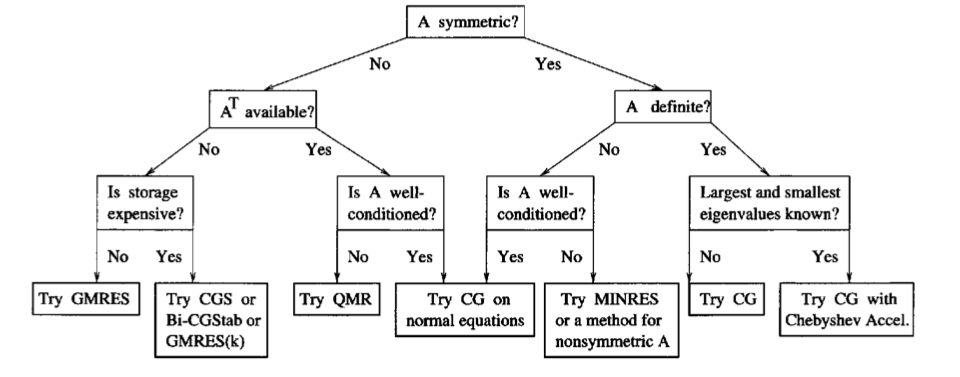
\includegraphics[width=14cm]{images/lec14-1.png}
    \caption{Decision tree for choosing an iterative algorithm for $Ax = b$.}
\end{figure}

Unlike Jacobi, GS and SOR, a Krylov subspace method for $Ax=b$ or $Ax = \lambda x$ need only a "black-box" subroutine to multiply $A$ times a vector by $x$ 
(or $A^\top$ times x, for some methods). So you do not need to ask for the diagonal part, or subdiagonal part, etc. that you would need for methods like Jacobi.

This is particularly useful in two situations:\begin{enumerate}
    \item You can write algorithms that are very general, can access $A$ only through subroutine for $Ax$.
    \item You can solve problems where $A$ may not actually be represented as a matrix with explicit entries, e.g. arises from doing a complicated simulation.
    For example, suppose you have a system, like a car engine or airplane wing, governed by a complicated set of PDEs. 
    You'd like to optimize some set $y$ of $n$ outputs of the PDE as a function of some set $x$ of $n$ inputs, $y=f(x)$, 
    say the pressure on the wing as a function of its shape. For some optimization methods, 
    this means that you need to solve linear systems with the $n\times n$ coefficient matrix $A = \nabla f$.
    $A$ is not written down, it is define implicitly as the derivative of the outputs of the simulation with respect to its inputs, and varies depending on the inputs. 
    The easiest way to access $A$ is to note that \begin{align*}
        Az = \nabla fz \sim \frac{(f(x + hz) - f(x))}{h}
    \end{align*}
    when $h$ is small enough, so multiplication by $A$ requires running the simulation twice to get $f(x + hz)$ and $f(x)$ 
    (care must be taken in choosing $h$ small enough but not too small, because otherwise the result is dominated by error).
    There is no such simple way to get $A^\top z$, unfortunately. There is actually software that takes an arbitrary collection of $C$ or
    Fortran subroutines computing an arbitrary function y = $f(x)$, and produces new $C$ or Fortran subroutines that compute $\nabla f(x)$, by differentiating
    each line of code automatically. A specialized and widely used example, for training neural nets, is TensorFlow.
\end{enumerate}





On the other hand, if we assume that the matrix $A$ is available explicitly, 
then it is possible to reorganize many Krylov subspace methods to significantly reduce their communication costs, 
which are dominated by moving the data needed to represent the sparse matrix $A$. For example, when $A$ is too large to fit in cache (a typical situation), 
each step of a conventional sequential method does a multiplication $Ax$, which requires reading the matrix $A$ from slow memory to cache.
Thus the communication cost is proportional to the number of steps, call it $k$.
However the reorganized Krylov subspace methods can take $k$ steps and only read $A$ from slow memory once, a potential speedup of a factor of $k$.
See \href{http://journals.cambridge.org/action/displayAbstract?fromPage=online&aid=9260756&fileId=S0962492914000038}{"Communication lower bounds and optimal algorithms for numerical linear algebra"} for more details. 
In practice $k$ is limited by both the sparsity structure of $A$ and issues of numerical stability.

We begin by discussing how to extract information about $A$ from a subroutine that does $Az$. Given a starting vector $y_1$ (say $y_1 = b$ for solving $Ax=b$),
we can compute $y_2 = Ay_1$, ... , $y_{i+1} = Ay_i$, ... $y_n = Ay_{n-1} = A^{n-1}y_1$.
Letting $K = [y_1,y_2,\cdots,y_n]$ we get \begin{align*}
    AK = \left[ Ay_{1},\cdots,Ay_{n} \right] = \left[ y_2, y_3, \cdots, A^n y_1 \right]
\end{align*}
Assuming for a moment that $K$ is nonsingular, write $c=-K^{-1} A^{n} y_1$ to get \begin{align*}
    Ak = K\left[ e_2, e_3, \cdots, e_n, -c \right] = KC
\end{align*}
where \begin{align*}
    C = k^{-1} A K= \left[ \begin{array}{cccc}
        0 & 0 & & -c_1 \\
        1 & 0 & & -c_2 \\
        0 & 1 & & -c_3 \\
        \vdots & \vdots & \ddots & \vdots \\
        \vdots & \vdots & & -c_n \\
    \end{array} \right]
\end{align*}
is upper Hessenberg, and a companion matrix, i.e. its characteristic polynomial is simply \begin{align*}
    p(x) = x^n + \sum_{i=1}^{n} c_i x^{i-1}.
\end{align*}
So just by matrix-vector multiplication we have reduced $A$ to a simple form, and could imagine using $C$ to solve $Ax=b$ or find eigenvalues.
But this would be a bad idea for two reasons:\begin{enumerate}
    \item $K$ is likely to be dense (if $y_1$ is dense), and solving with $K$ is probably harder than solving with $A$.
    \item $K$ is likely to be very ill-conditioned, since it is basically running the power method, so the vectors $y_i$ are converging to the eigenvector of the largest eigenvalue in absolute value.
\end{enumerate}
Krylov subspace methods address these two drawbacks, implicitly or explicitly, as follows: 

We will not compute $K$ but rather an orthogonal $Q$ such that the leading $k$ columns of $K$ and of $Q$ span the same space, called a Krylov subspace: \begin{align*}
    \operatorname{span}\left\{ y_1, y_2, \cdots, y_k \right\} = \operatorname{span}\left\{ y_1, Ay_1, \cdots, A^{k-1}y_1 \right\} = \mathcal{K}_k(A, y_1)
\end{align*}
The relationship between $K$ and $Q$ is simply the QR decomposition: $K = QR$. Furthermore, we won't compute all $n$ columns of $K$ and $Q$, 
but just the first $k \ll n$ columns, and settle for the "best" approximate solution $x$ of $Ax=b$ or $Ax = \lambda x$ that we can find in the Krylov subspace
they span (the definition of "best" depends on the algorithm).

To proceed, substitute $K = QR$ into $C = K^{-1}AK$ to get \begin{align*}
    C = R^{-1}Q^\top AQR 
\end{align*} 
or \begin{align*}
    RCR^{-1} = Q^\top AQ = H && (\star)
\end{align*}
Since $R$ and $R^{-1}$ are triangular, and $C$ is upper Hessenberg, then $H$ is also upper Hessenberg. If $A$ is symmetric, then so is $H$, 
and so $H$ is tridiagonal.

To see how to compute the columns of $Q$ and $H$ one at a time, write $Q=\left[ q_1, q_2, \cdots, q_n \right]$, rewrite $(\star)$ as \begin{align*}
    AQ=QH
\end{align*}
and equate the $j$-th column on both sides to get \begin{align*}
    Aq_j = \sum_{i=1}^{j+1} q_i H(i,j)
\end{align*}
Since the $q_j$ are orthonormal, multiply both sides of the last equality by $q_m^\top$ to get \begin{align*}
    q_m^\top Aq_j = \sum_{i=1}^{j+1} H(i,j) q_m^\top q_i = H(m,j)
\end{align*}
for $1 \leq m \leq j$. And so \begin{align*}
    H(j+1,j)  q_{j+1} = A q_j - \sum_{i=1}^{j} q_i H(i,j).
\end{align*}
This yields the following algorithm:
\begin{algorithmfrm}[Arnoldi algorithm for (partial) reduction of $A$ to Hessenberg form]
    \begin{algorithmic}
        \State $ q_1 = y_1 / ||y_1||_2 $
        \For{$j=1:k$}
            \State $z = Aq_j$
            \For{$i=1:j$}\Comment{Run Modified Gram-Schmidt (MGS) on $z$}
                \State $H(i,j) = q_i^\top z$
                \State $z = z - H(i,j)q_i$
            \EndFor
            \State $H(j+1,j) = ||z||_2$
            \State $q_{j+1} = z / H(j+1,j)$
        \EndFor
    \end{algorithmic}
\end{algorithmfrm}
The $q_j$ vectors are called Arnoldi vectors, and the cost is $k$ multiplications by $A$, plus $O(k^2 n)$ flops for MGS. If we stop the algorithm here, at $k < n$, 
what have we learned about $A$? Write$ Q = [Q_k,Q_u]$ where $Q_k = [q_1, \cdots, q_k]$ is computed as well as the first column $q_{k+1}$ of $Q_u$; 
the other columns of $Q_u$ are unknown. Then \begin{align*}
    H &= Q^\top AQ = [Q_k,Q_u]^\top A [Q_k,Q_u] \\
    &= \left[\begin{array}{ll}
        Q_{k}^{\top} A Q_{k} & Q_{k}^{\top} A Q_{u} \\
        Q_{u}^{\top} A Q_{k} & Q_{u}^{\top} A Q_{u}
        \end{array}\right] \\
    &= \left[\begin{array}{ll}
        H_{k} & H_{u k} \\
        H_{ku} & H_{u}
        \end{array}\right]
\end{align*}
Since $H$ is upper Hessenberg, so are $H_k$ and $H_u$, and $H_{ku}$ has a single nonzero entry in its upper right corner, namely $H(k+1,k)$.
So $H_{uk}$ and $H_u$ are unknown, and $H_k$ and $H_{ku}$ are known. When A is symmetric, so that H is symmetric and tridiagonal, we may write \begin{align*}
    H=T=\begin{bmatrix}
        \alpha_1 & \beta_1 &  & O \\ 
        \beta_1 & \alpha_2 & \beta_2 & \\ 
        & \beta_2 & \alpha_3 & \ddots \\ 
        &  & \ddots & \ddots \\ 
        O &  &  & \alpha_n
       \end{bmatrix}
\end{align*}
Equating column $j$ on both sides of $AQ = QT$ yields
\begin{align*}
    Aq_j = \beta_{j-1}q_{j-1} + \alpha_j q_j + \beta_j q_{j-1}
\end{align*}
Multiplying both sides by $q_j^\top$ yields \begin{align*}
    q_j^\top A q_j = \alpha_j,
\end{align*}
which leading to the following simpler version of the Arnoldi algorithm, called Lanczos:
\begin{algorithmfrm}[Lanczos algorithm for (partial) reduction of $A=A^\top$ to tridiagonal form]
    \begin{algorithmic}
        \State $q_1 = y_1 / ||y_1||_2$
        \State $\beta_0=0$
        \State $q_0=0$
        \For{$j=1:k$}
            \State $z = Aq_j$
            \State $\alpha_j = q_j^\top z$
            \State $z = z - \alpha_j q_j - \beta_{j-1}q_{j-1}$
            \State $\beta_j = ||z||_2$
            \State $q_{j+1} = z / \beta_j$
        \EndFor
    \end{algorithmic}
\end{algorithmfrm}
Here is some notation to describe the Arnoldi and Lanczos algorithms. As above, the space spanned by $\left\{ q_1,\cdots,q_k \right\}$ is called a Krylov subspace:
\begin{align*}
    \mathcal{K}_k (A,y_1) = \operatorname{span}\left\{ q_1,\cdots,q_k \right\}
\end{align*}
or $\mathcal{K}_k$ for short. We call $H_k$ ($T_k$ for Lanczos) the projection of $A$ onto $\mathcal{K}_k$.

Our goal is to solve $Ax=b$ or $Ax = \lambda x$ by somehow finding the "best" solution in the Krylov subspace. For the eigenvalue problem, the answer is simple: 
use the eigenvalues of $H_k$ (or $T_k$) as approximate eigenvalues of $A$. To see what the error is, suppose $H_k y = \lambda y$ and write \begin{align*}
    H \left[ \begin{array}{cc}
        y \\ 0
    \end{array} \right]  = \left[\begin{array}{ll}
        H_{k} & H_{u k} \\
        H_{ku} & H_{u}
        \end{array}\right]\left[ \begin{array}{cc}
            y \\ 0
        \end{array} \right] = \left[ \begin{array}{cc}
            H_k y \\ H_{ku}y
        \end{array} \right] = \left[ \begin{array}{cc}
            \lambda y \\ H_{k+1, k} y_k e_1
        \end{array} \right]
\end{align*}
and since $AQ = QH$, \begin{align*}
    A Q\left[ \begin{array}{cc}
        y \\ 0
    \end{array} \right]  = \lambda Q\left[ \begin{array}{cc}
        y \\ 0
    \end{array} \right] + q_{k+1} H_{k+1, k} y_k
\end{align*}
so if the product of $H_{k+1, k} y_k$ is small, the eigenvalue/vector pair $(\lambda, y') = (\lambda, Q[y, 0]^\top)$ has a small residual \begin{align*}
    || Ay' - \lambda y' ||_2 = |H_{k+1, k} y_k|
\end{align*}
When $A$ is symmetric, we know that this is in fact a bound on the error in $\lambda$.

To see how the eigenvalues of $T_k$ approximate the eigenvalues of $A$ as $k$ grows, we consider the symmetric case (Lanczos), 
and plot the eigenvalue of $T_k$ versus $k$.

\begin{figure}[h]
    \centering
    \begin{subfigure}{.5\textwidth}
      \centering
      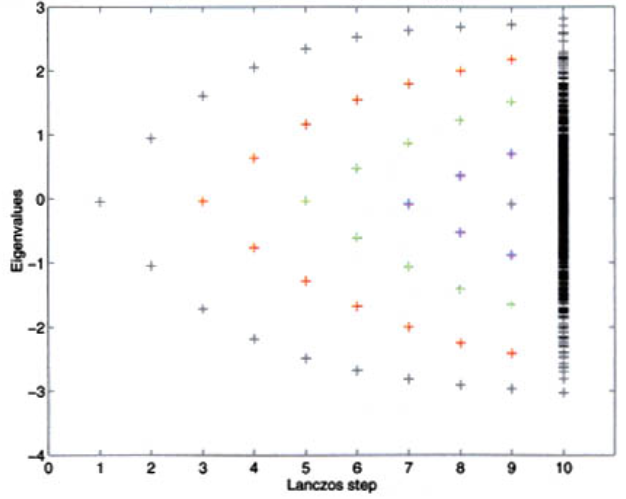
\includegraphics[width=.9\linewidth]{images/lec14-2.png}
      \caption{9 steps}
    \end{subfigure}%
    \begin{subfigure}{.5\textwidth}
      \centering
      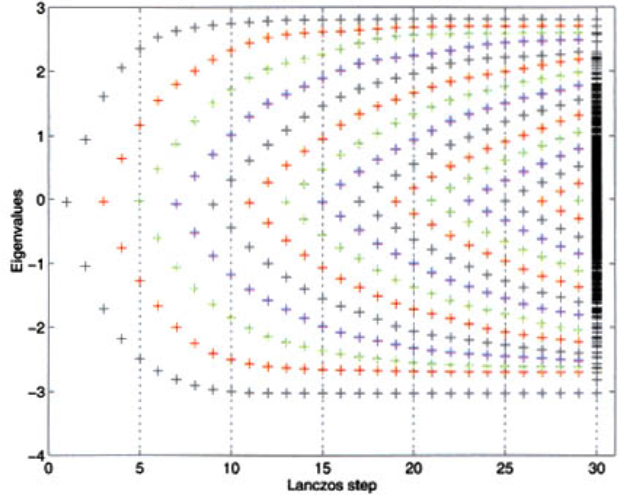
\includegraphics[width=.9\linewidth]{images/lec14-3.png}
      \caption{29 steps}
    \end{subfigure}
    \caption{The Lanczos algorithm (full reorthogonalization) applied to $A$ with different numbers of steps. Column $k$ shows the eigenvalues of $T_k$, 
    except that the rightmost columns show all the eigenvalues of $A$.}
\end{figure}

This lecture has ignored floating point errors so far. In practice, it is common for the vectors $q_j$ to lose orthogonality as the number of iterations grows, 
leading to more complicated behavior, and interesting algorithmic changes.

\end{document}
